% !TeX program = xelatex
% A业务建模、B需求与C分析按完整日常诊所业务同步。
% 可使用安装了 ctex 的 XeLaTeX 编译（Windows 宋体、黑体）。
% 本机验证工具：D:\CS\latex_Tectonic\tectonic.exe
% Tectonic 使用现有缓存：--only-cached --bundle http://127.0.0.1:8765/tlextras-2022.0r0.tar
% 无字体配置时，在 PowerShell 中设置：
% $fc=Join-Path $env:TEMP 'dental-tectonic-fonts.conf'
% '<fontconfig><dir>C:/Windows/Fonts</dir></fontconfig>' | Set-Content -LiteralPath $fc -Encoding utf8
% $env:FONTCONFIG_FILE=$fc
\documentclass[UTF8,a4paper,zihao=-4,fontset=none]{ctexart}
\setmainfont{Times New Roman}
\setCJKmainfont{SimSun}[BoldFont=SimHei,ItalicFont=KaiTi]
\setCJKsansfont{SimHei}
\usepackage[margin=2.5cm,headheight=15pt]{geometry}
\usepackage{booktabs,tabularx,longtable,array,fancyhdr,graphicx}
\usepackage[hidelinks]{hyperref}
\setlength{\parindent}{2em}
\setlength{\parskip}{0.25em}
\linespread{1.15}
\ctexset{
  section={name={,、},number=\chinese{section},format=\Large\bfseries},
  subsection={format=\large\bfseries},
  subsubsection={format=\normalsize\bfseries}
}
\pagestyle{fancy}
\fancyhf{}
\fancyhead[L]{\small 牙科诊所管理系统}
\fancyhead[R]{\small 需求文档}
\fancyfoot[C]{\small \thepage}
\renewcommand{\headrulewidth}{0.4pt}
\newcolumntype{L}{>{\raggedright\arraybackslash}X}
\hypersetup{pdftitle={牙科诊所管理系统-需求文档},pdfauthor={青禾牙科诊所},pdfsubject={业务建模、需求与分析}}

\begin{document}
\begin{center}
  {\Large\bfseries 牙科诊所管理系统需求文档}\par\vspace{0.3em}
  {\small 业务建模、需求与分析\qquad 2026年10月9日}
\end{center}
\tableofcontents
\clearpage

\section{业务建模}
\subsection{愿景}

\subsubsection{目标组织与业务背景}
青禾牙科诊所是一家位于学校周边的单店牙科诊所，面向周边居民及师生提供口腔检查、诊断、治疗和诊后服务。诊所配置6名工作人员：2名牙医（其中1名兼任负责人）、2名诊疗助理、1名前台和1名收费人员。

患者可以提前预约，也可以到诊后由前台协调接诊。前台核对身份及联系方式，建立或查找患者资料，确认接诊牙医和候诊安排。牙医了解就诊原因及相关病史，查阅既往诊疗资料，进行口腔检查，记录牙位、检查所见及诊断；随后向患者说明治疗方案、预计安排及费用，患者确认后进入相应治疗。仅需检查咨询或尚未确认方案的患者，可以在检查与说明完成后结束当次诊疗。

治疗由牙医实施，诊疗助理负责诊前准备和诊疗协助。牙医记录实际治疗经过、完成的项目及诊后注意事项；收费人员依据已确认的项目和适用价目核对费用，办理收款并交付结算凭据。需要继续治疗或复查的患者，由牙医提出后续安排，前台联系患者并协调复诊；复诊时查阅前次记录，评估恢复情况或继续既定治疗，使多次就诊保持连续。

诊所日常运行还包括接诊人员安排、收费价目确认、诊疗材料补充与领用、器械清洁消毒以及就诊和收款核对。各岗位的主要业务职责见表\ref{tab:business-roles}。预约记录、患者资料、诊疗记录、结算凭据和复诊安排共同构成业务办理依据；这些资料分散、转录和交接不及时，会增加重复询问及跨岗位核实。诊所需要贯通患者服务过程，使接诊、诊疗、收费与复诊能够使用一致的业务信息。

\begin{table}[!htbp]
\centering
\caption{诊所岗位与主要业务职责}
\label{tab:business-roles}
\small
\renewcommand{\arraystretch}{1.18}
\begin{tabularx}{\textwidth}{@{}p{2.4cm}L@{}}
\toprule
岗位 & 主要业务职责 \\
\midrule
前台 & 联系与接待患者；协调预约和到诊安排；核对患者资料；交接就诊信息；联系患者并安排复诊。 \\
牙医 & 检查诊断；说明方案与费用；实施治疗；记录诊疗经过及已完成项目；提供诊后指导；评估复诊情况。 \\
诊疗助理 & 准备诊疗环境、器械和材料；协助牙医治疗；整理诊疗物品；办理材料领用及诊后清洁消毒。 \\
收费人员 & 依据确认价目核算费用；核对项目与金额；办理收款并交付凭据；核对当日收款。 \\
诊所负责人 & 协调人员及接诊能力；确认收费价目；安排材料补充；查看就诊、收款和服务运行情况。 \\
\bottomrule
\end{tabularx}
\end{table}

\clearpage
\subsubsection{愿景表}

\begin{table}[htbp]
\centering
\caption{牙科诊所管理系统愿景}
\label{tab:vision}
\renewcommand{\arraystretch}{1.28}
\begin{tabularx}{\textwidth}{@{}p{2.3cm}L@{}}
\toprule
项目 & 内容 \\
\midrule
系统 & 牙科诊所管理系统。 \\
目标组织 & 青禾牙科诊所（单店、6名工作人员）。 \\
目标 & 缩短患者单次就诊中，到诊接待与费用结算的平均办理时长。 \\
度量指标 & 同一统计期内，完成到诊接待与费用结算的各次就诊，其两段办理时长之和的平均值，单位为分钟/次。 \\
对比时间 & 以系统启用前连续4周为基准期，启用后第5至第8周为对比期。第1至第4周为使用适应期；统计起止日期根据启用日预先确定。 \\
改进值 & 对比期平均办理时长较基准期降低至少20\%。该比例为预期改进目标，实际结果按统一口径统计。 \\
\bottomrule
\end{tabularx}
\end{table}

\newpage
\subsubsection{度量口径}
为使愿景中的改进能够比较，按一次就诊分别记录以下四个时点。两段办理过程中的资料核对、重复录入和岗位间核实所用时间均计入。

\begin{table}[htbp]
\centering
\caption{接待与结算办理时长的计时口径}
\label{tab:measure}
\renewcommand{\arraystretch}{1.3}
\begin{tabularx}{\textwidth}{@{}>{\raggedright\arraybackslash}p{2.7cm}>{\raggedright\arraybackslash}p{1.8cm}L@{}}
\toprule
业务环节 & 时点符号 & 时点定义 \\
\midrule
到诊接待开始 & a & 前台开始为本次就诊办理预约及身份资料核对的时刻。 \\
到诊接待结束 & b & 前台完成接待登记并告知患者候诊安排的时刻。 \\
费用结算开始 & c & 收费人员开始为该次就诊核对治疗项目和费用的时刻。 \\
费用结算结束 & d & 收费人员完成该次收款登记、交付结算凭据，并向患者确认本次结清的时刻。 \\
\bottomrule
\end{tabularx}
\end{table}

单次办理时长为接待时长（b减a）与结算时长（d减c）之和，各时差统一换算为分钟。统计期的平均办理时长按下式计算：
\begin{center}
平均办理时长＝纳入统计的各次办理时长之和÷纳入统计的就诊次数。
\end{center}
本愿景以平均办理时长降低至少20\%为达到目标的条件。统计窗口在系统启用时确定，评价时不因结果改变窗口。基准期平均值大于零时，降低比例按下式计算：
\begin{center}
降低比例＝（基准期平均值－对比期平均值）÷基准期平均值×100\%。
\end{center}

统计以一次就诊为单位，同一患者多次就诊分别计数。只纳入到诊接待与当次结算均完成、四个时点均有记录的就诊；未到诊、取消或计时不完整的记录不纳入，并说明排除数量和原因。两期均使用相同口径，同时报告就诊次数、初复诊构成及人员配置变化，以说明比较条件。任一期没有符合口径的记录时，不计算改进比例。

本指标统计当次足额结清的就诊，不包含开始接待前的排队时间、接待完成后的候诊时间、诊断治疗时间及开始结算前的排队时间。尚未结清或计时不完整的就诊不纳入，并单列排除数量。


\clearpage
\subsection{业务用例图}

青禾牙科诊所的对外业务包括预约就诊、口腔检查与诊断、口腔治疗、复诊与随访以及费用结算。图\ref{fig:business-use-case}呈现患者能够从诊所获得的各项业务结果；表\ref{tab:business-support}列出实现这些结果所需的内部支持工作。

\begin{figure}[htbp]
\centering
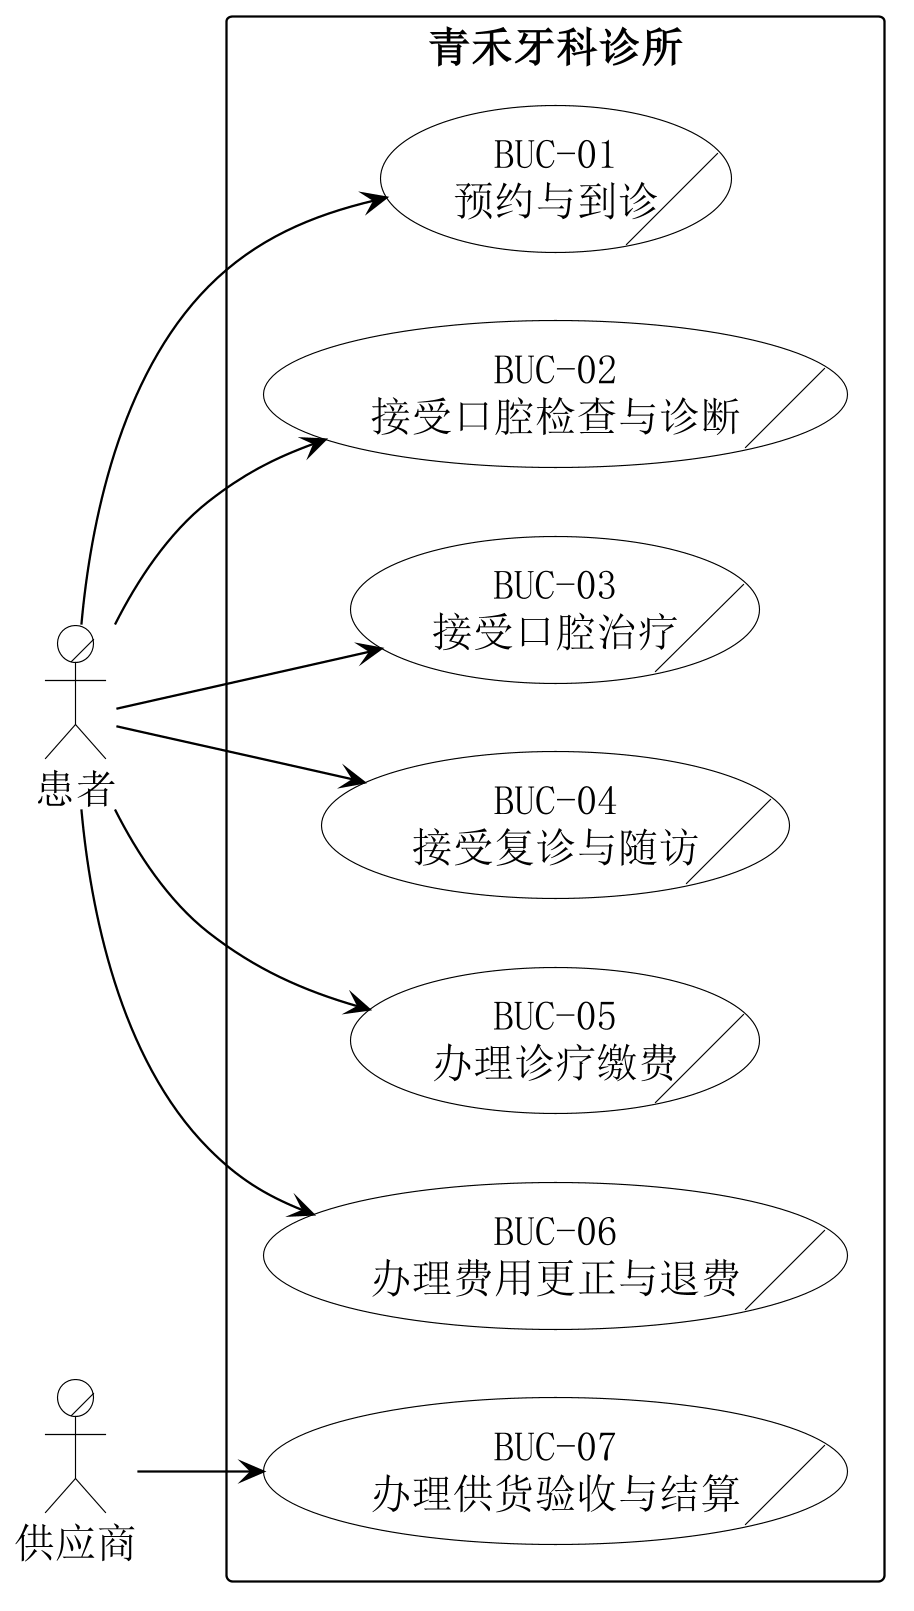
\includegraphics[width=0.92\textwidth,height=10.5cm,keepaspectratio]{diagrams/01-business-use-case.png}
\caption{青禾牙科诊所业务用例图}
\label{fig:business-use-case}
\end{figure}

\begin{table}[htbp]
\centering
\caption{业务用例说明}
\label{tab:business-use-cases}
\small
\renewcommand{\arraystretch}{1.2}
\begin{tabularx}{\textwidth}{@{}>{\raggedright\arraybackslash}p{1.9cm}>{\raggedright\arraybackslash}p{2.9cm}L@{}}
\toprule
编号 & 业务用例 & 向患者提供的业务结果 \\
\midrule
BUC-01 & 预约就诊 & 患者获得确认的就诊时间和接诊安排；需要时可以与诊所协调调整或取消预约。 \\
BUC-02 & 接受口腔检查与诊断 & 患者获得检查结果、诊断说明及可选择的治疗方案和费用说明。 \\
BUC-03 & 接受口腔治疗 & 患者获得双方确认的相应治疗、实际治疗结果及诊后指导。 \\
BUC-04 & 接受复诊与随访 & 患者获得恢复情况或治疗效果的复核、后续处理意见及继续诊疗的安排。 \\
BUC-05 & 结算诊疗费用 & 患者核对已完成项目及费用，完成付款并获得明细与结算凭据。 \\
\bottomrule
\end{tabularx}
\end{table}

患者可以在完成检查与诊断后决定是否接受治疗；需要分次治疗或复查时，再办理后续就诊安排。费用按当次实际完成的项目结算。到诊接待连接预约与检查诊断，诊疗记录连接治疗、收费和复诊；一次就诊可以涉及多个业务用例。



\clearpage
\subsubsection{独立业务用例图}

以下各图分别对应BUC-01至BUC-05。

\begin{figure}[htbp]
\centering
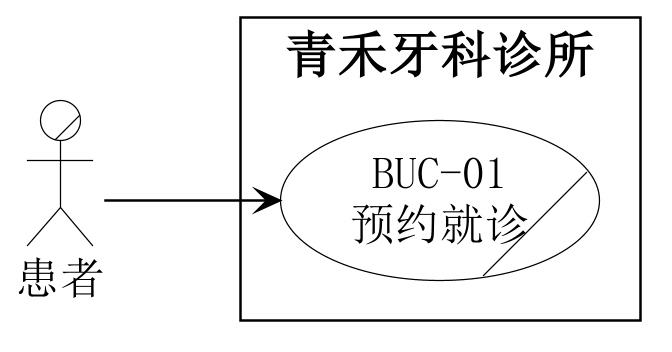
\includegraphics[width=0.85\textwidth,height=3.4cm,keepaspectratio]{diagrams/01-01-business-use-case.png}
\caption{BUC-01 预约就诊业务用例图}
\label{fig:buc-01}
\end{figure}
患者提出预约需求，诊所确认接诊安排，双方约定就诊时间。

\begin{figure}[htbp]
\centering
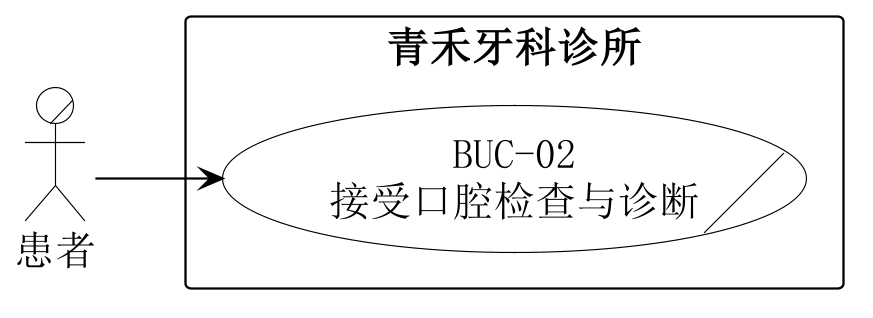
\includegraphics[width=0.85\textwidth,height=3.4cm,keepaspectratio]{diagrams/01-02-business-use-case.png}
\caption{BUC-02 接受口腔检查与诊断业务用例图}
\label{fig:buc-02}
\end{figure}
患者说明就诊原因，牙医结合病史与口腔检查给出诊断，向患者说明治疗方案、安排及费用。检查结果和方案形成后续诊疗依据。

\begin{figure}[htbp]
\centering
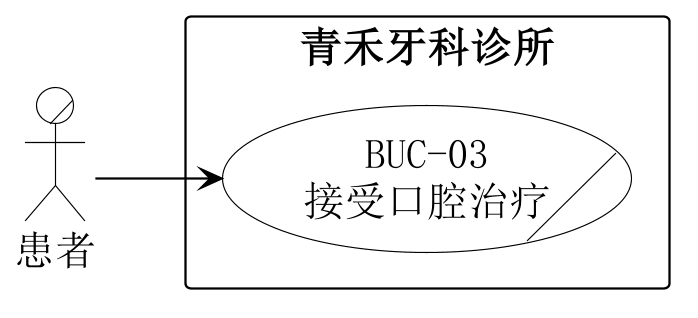
\includegraphics[width=0.85\textwidth,height=3.4cm,keepaspectratio]{diagrams/01-03-business-use-case.png}
\caption{BUC-03 接受口腔治疗业务用例图}
\label{fig:buc-03}
\end{figure}
患者确认治疗安排，牙医在诊疗助理配合下实施治疗，记录实际治疗经过及完成项目，并向患者交代诊后注意事项和后续安排。

\clearpage
\begin{figure}[htbp]
\centering
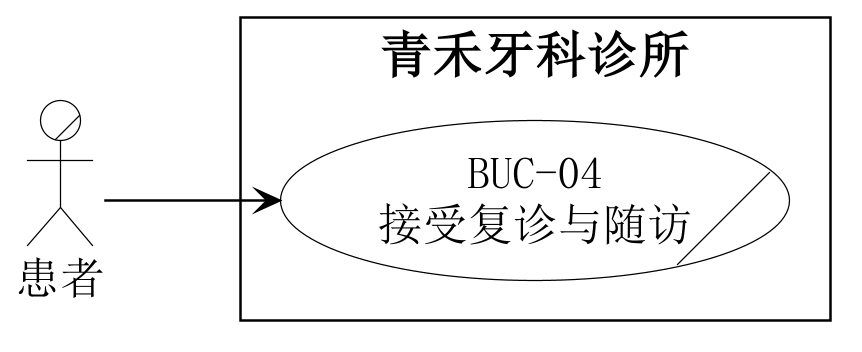
\includegraphics[width=0.85\textwidth,height=3.4cm,keepaspectratio]{diagrams/01-04-business-use-case.png}
\caption{BUC-04 接受复诊与随访业务用例图}
\label{fig:buc-04}
\end{figure}
牙医提出复诊或随访要求，前台联系患者并协调安排。牙医查阅前次诊疗资料，评估恢复情况、继续治疗或给出后续意见，记录本次结果。

\begin{figure}[htbp]
\centering
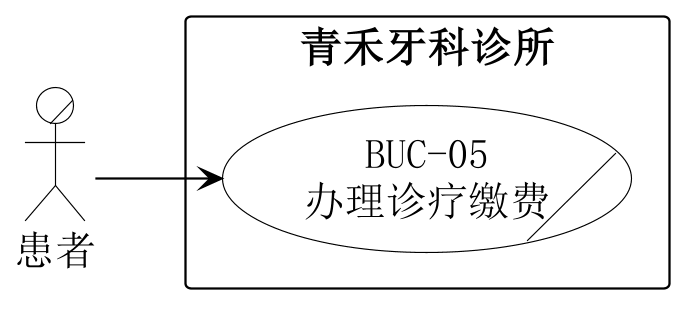
\includegraphics[width=0.85\textwidth,height=3.4cm,keepaspectratio]{diagrams/01-05-business-use-case.png}
\caption{BUC-05 结算诊疗费用业务用例图}
\label{fig:buc-05}
\end{figure}
收费人员依据牙医确认的已完成项目及适用价目计算费用，与患者核对后办理收款，交付费用明细及结算凭据。

\clearpage
\subsubsection{业务支持与岗位协作}

人员安排、诊疗资料、器械材料和收款核对贯穿患者服务。诊所负责人协调接诊能力并确认价目；前台、牙医、助理和收费人员承担各自的办理与交接责任。

\begin{table}[!htbp]
\centering
\caption{内部业务工作与患者业务结果的对应}
\label{tab:business-support}
\small
\renewcommand{\arraystretch}{1.25}
\begin{tabularx}{\textwidth}{@{}>{\raggedright\arraybackslash}p{2.4cm}>{\raggedright\arraybackslash}p{2.6cm}L>{\raggedright\arraybackslash}p{2.0cm}@{}}
\toprule
业务工作 & 负责岗位 & 工作结果 & 支持用例 \\
\midrule
接诊人员安排 & 负责人、牙医、前台 & 明确可接诊人员与时段，预约与现场接待使用一致安排。 & BUC-01至04 \\
患者资料与诊疗记录 & 前台、牙医 & 身份资料与各次诊疗关联，保留病史、检查诊断、方案、治疗经过及诊后要求。 & BUC-01至05 \\
器械与材料保障 & 负责人、诊疗助理 & 完成材料入库、领用与盘点，备齐诊疗物品，并完成器械清洁消毒。 & BUC-02、03、04 \\
收费价目管理 & 负责人、收费人员 & 确认项目价格与适用时间，保留费用计算依据。 & BUC-02、03、05 \\
复诊联系与安排 & 牙医、前台 & 复诊要求有明确来源，联系和预约结果可以回查，并关联前次诊疗。 & BUC-01、04 \\
业务与收款核对 & 负责人、收费人员 & 核对接诊、诊疗与收款情况，发现漏记或不一致并交相关岗位处理。 & BUC-01至05 \\
\bottomrule
\end{tabularx}
\end{table}

\clearpage
\subsection{现状业务序列图}

现状业务由前台、牙医、诊疗助理、收费人员及负责人协作完成，预约、诊疗和收费主要通过纸质资料记录与交接。以下分别描述患者服务及内部管理的典型业务场景。

\subsubsection{预约安排现状}

患者通过电话或到店提出预约需求。前台询问就诊需求及联系方式，查阅接诊安排并向牙医核实可用时段，与患者约定后在预约本登记。调整或取消预约时，前台同步修改纸质记录并告知相关人员。

\begin{figure}[!htbp]
\centering
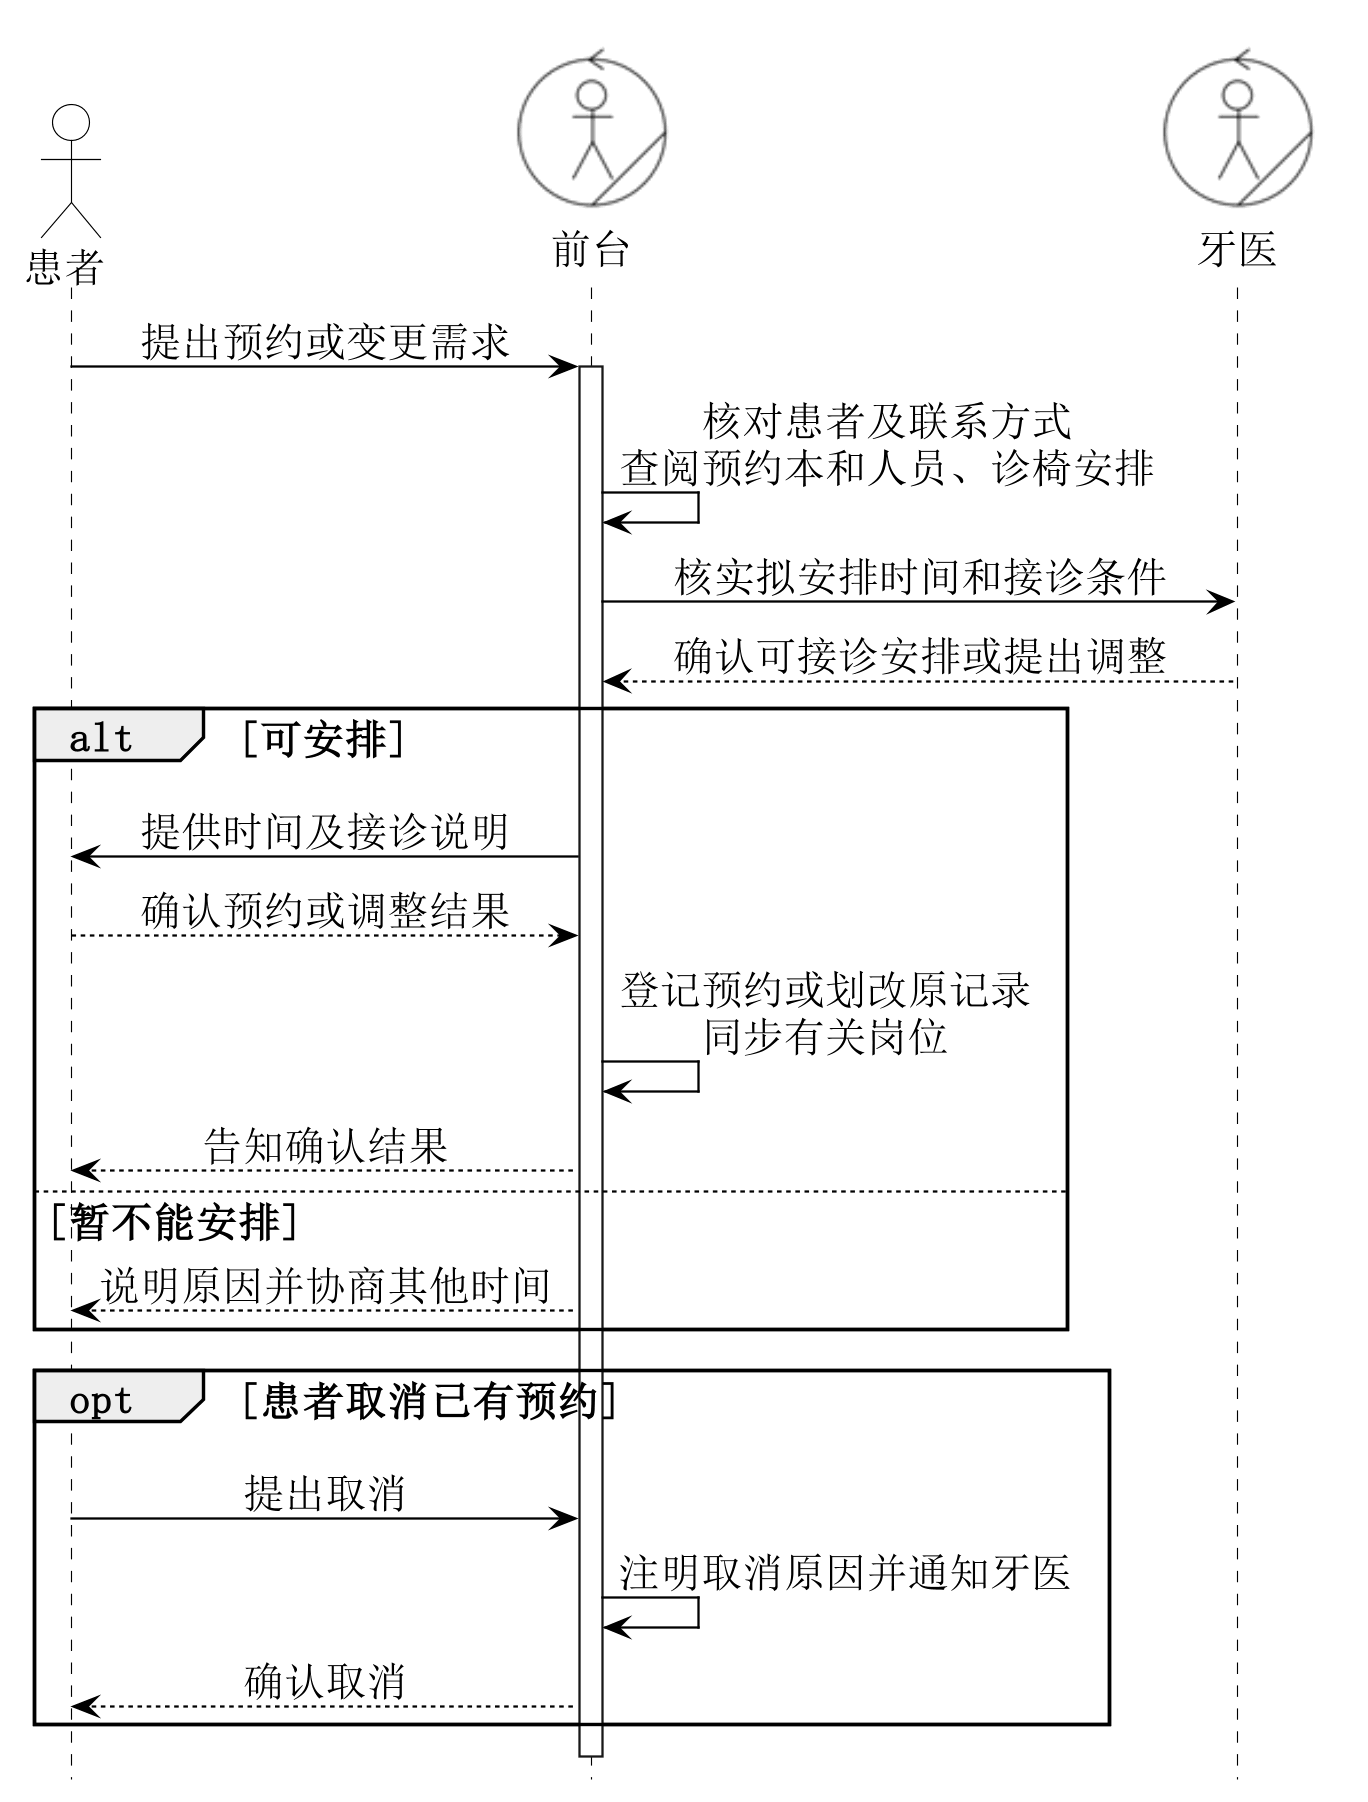
\includegraphics[width=\textwidth,height=13.8cm,keepaspectratio]{diagrams/02c-as-is-appointment.png}
\caption{现状业务序列图：预约安排}
\label{fig:as-is-appointment}
\end{figure}

患者获得明确的就诊时间与接诊安排，前台保留后续接待所需的预约依据。

\clearpage
\subsubsection{到诊接待现状}

本片段连接BUC-01与BUC-02。已预约患者按约到诊，前台查找预约本，核对身份和预约信息，向牙医确认接诊安排，再抄录到诊信息并告知候诊安排。未预约患者先由前台协调接诊，本图展开已预约且记录可查的场景。

\begin{figure}[!htbp]
\centering
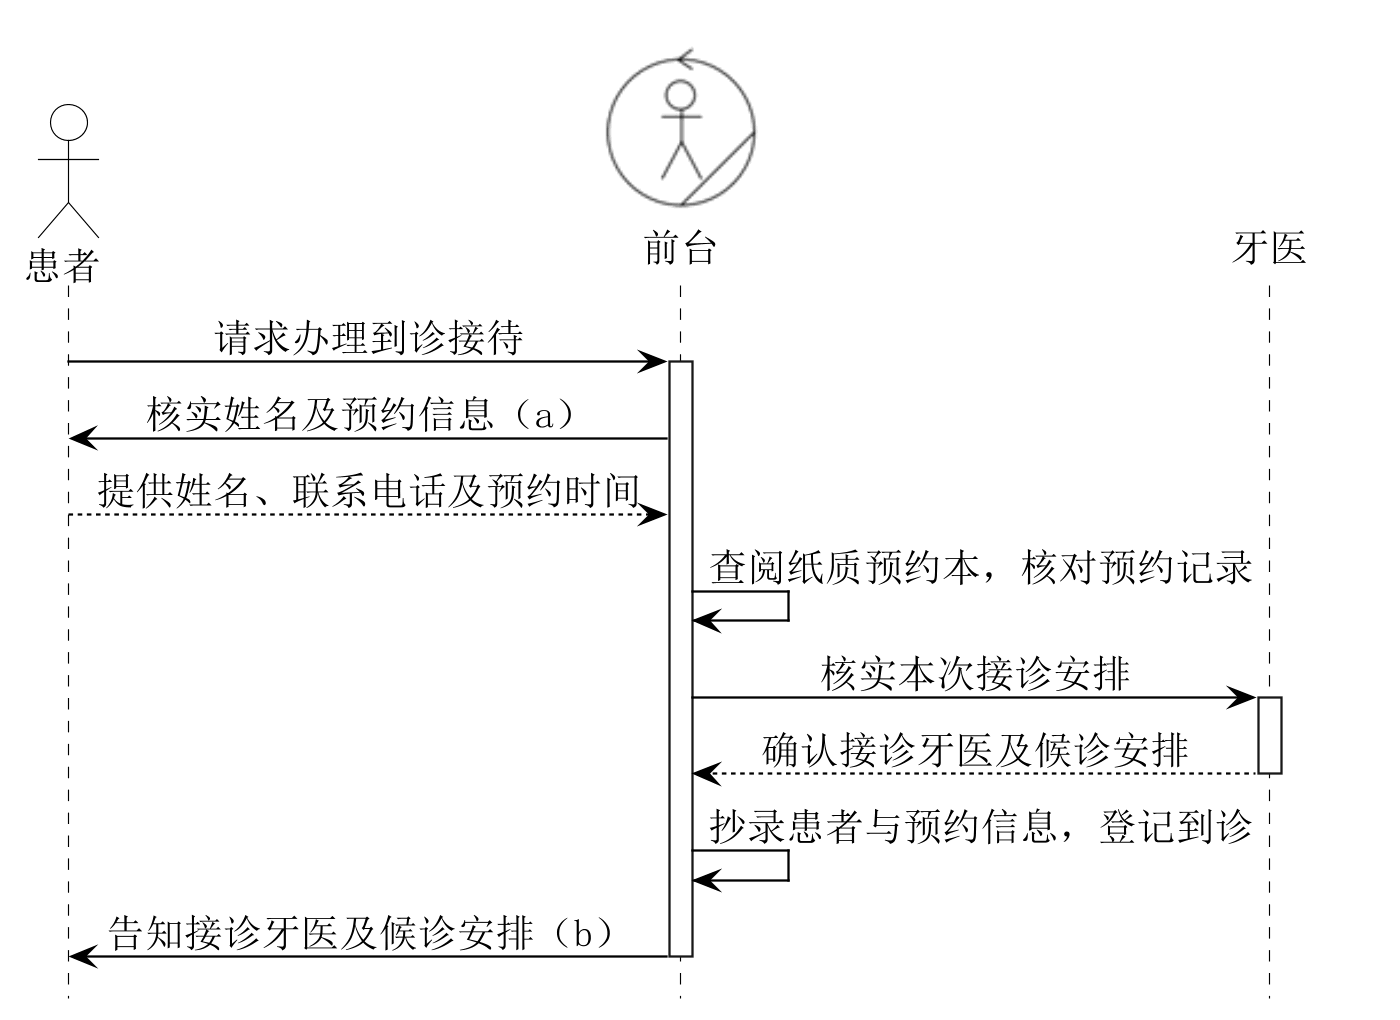
\includegraphics[width=\textwidth,height=11.3cm,keepaspectratio]{diagrams/02-as-is-business-sequence.png}
\caption{现状业务序列图：到诊接待}
\label{fig:as-is-reception}
\end{figure}

图中a为开始核对身份与预约的时点，b为到诊登记和候诊告知完成的时点，对应愿景中的接待办理时长。

\clearpage
\subsubsection{检查诊断与治疗现状}

本场景对应BUC-02和BUC-03。牙医查阅纸质患者资料，询问主诉和相关病史，完成口腔检查并说明诊断、治疗方案、安排及费用。患者确认后，助理准备器械材料并配合牙医实施治疗；牙医填写病历、已完成项目及诊后要求。仅接受检查或暂未确认方案的患者，可以不进入治疗环节。

\begin{figure}[!htbp]
\centering
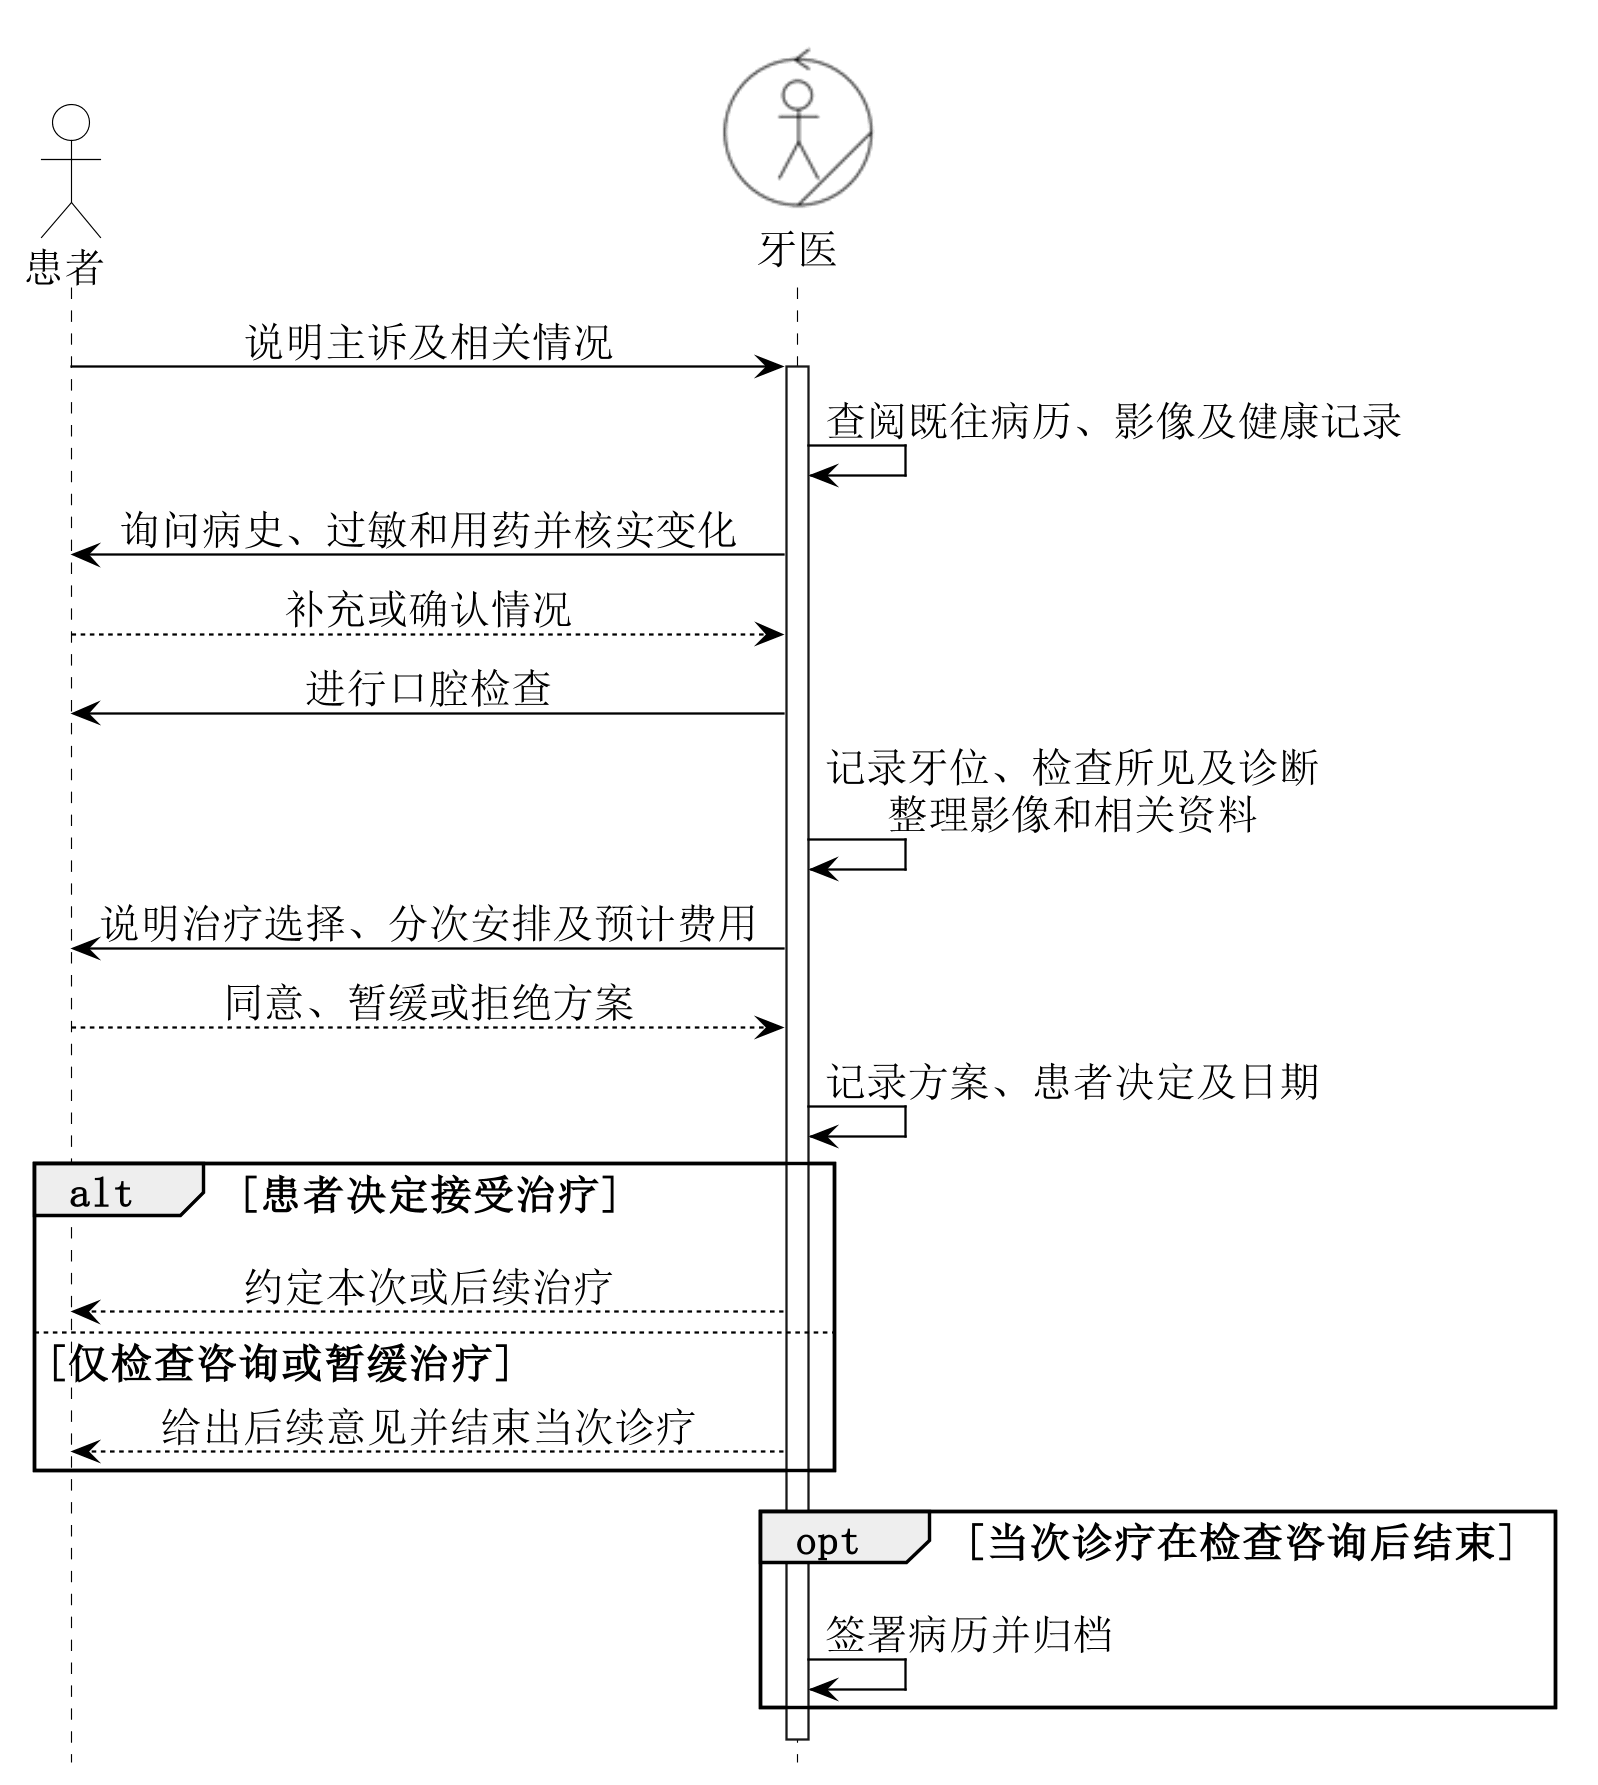
\includegraphics[width=\textwidth,height=15.5cm,keepaspectratio]{diagrams/02d-as-is-clinical.png}
\caption{现状业务序列图：检查诊断与治疗}
\label{fig:as-is-clinical}
\end{figure}

牙医承担检查诊断、方案沟通和治疗责任；助理承担准备与协助责任。治疗记录反映实际发生的诊疗，不以收费项目清单代替病历。

\clearpage
\subsubsection{费用结算现状}

本片段属于BUC-05。本次诊疗完成，牙医填写纸质诊疗单，患者持单办理结算。收费人员向牙医核实已完成项目及数量，查价计算费用，与患者核对后收款、登记并交付收据。本图展开患者认可费用并以现金足额结清的场景。

\begin{figure}[!htbp]
\centering
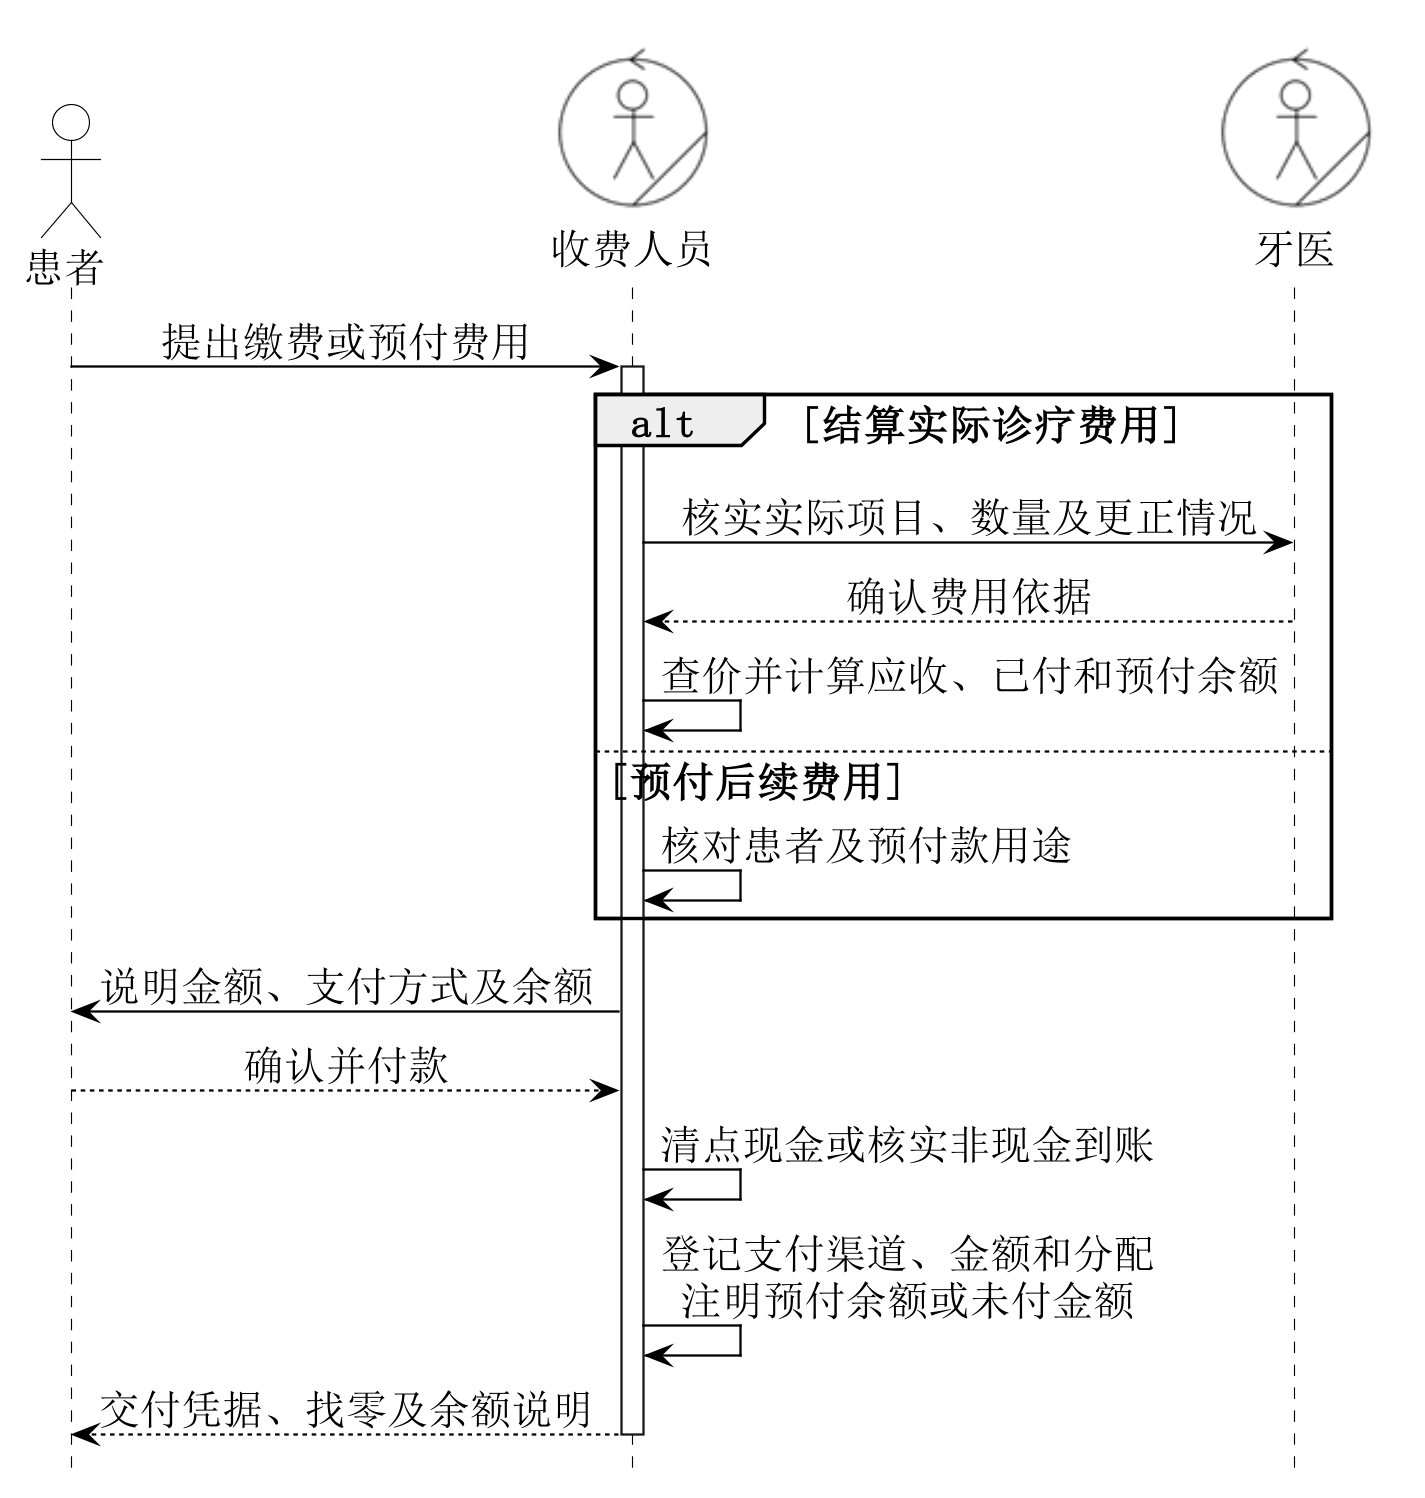
\includegraphics[width=\textwidth,height=13.0cm,keepaspectratio]{diagrams/02b-as-is-billing-sequence.png}
\caption{现状业务序列图：费用结算}
\label{fig:as-is-billing}
\end{figure}

图中c为开始核对本次患者与诊疗费用的时点，d为收款登记、凭据及找零交付完成的时点，对应愿景中的结算办理时长。

\clearpage
\subsubsection{复诊与随访现状}

本场景对应BUC-04。牙医在前次诊疗记录中提出复诊或随访要求，前台依据纸质记录联系患者，记录联系结果并安排复诊。患者复诊时，牙医查阅前次资料，评估恢复情况或继续治疗，给出后续意见并补记本次结果。

\begin{figure}[!htbp]
\centering
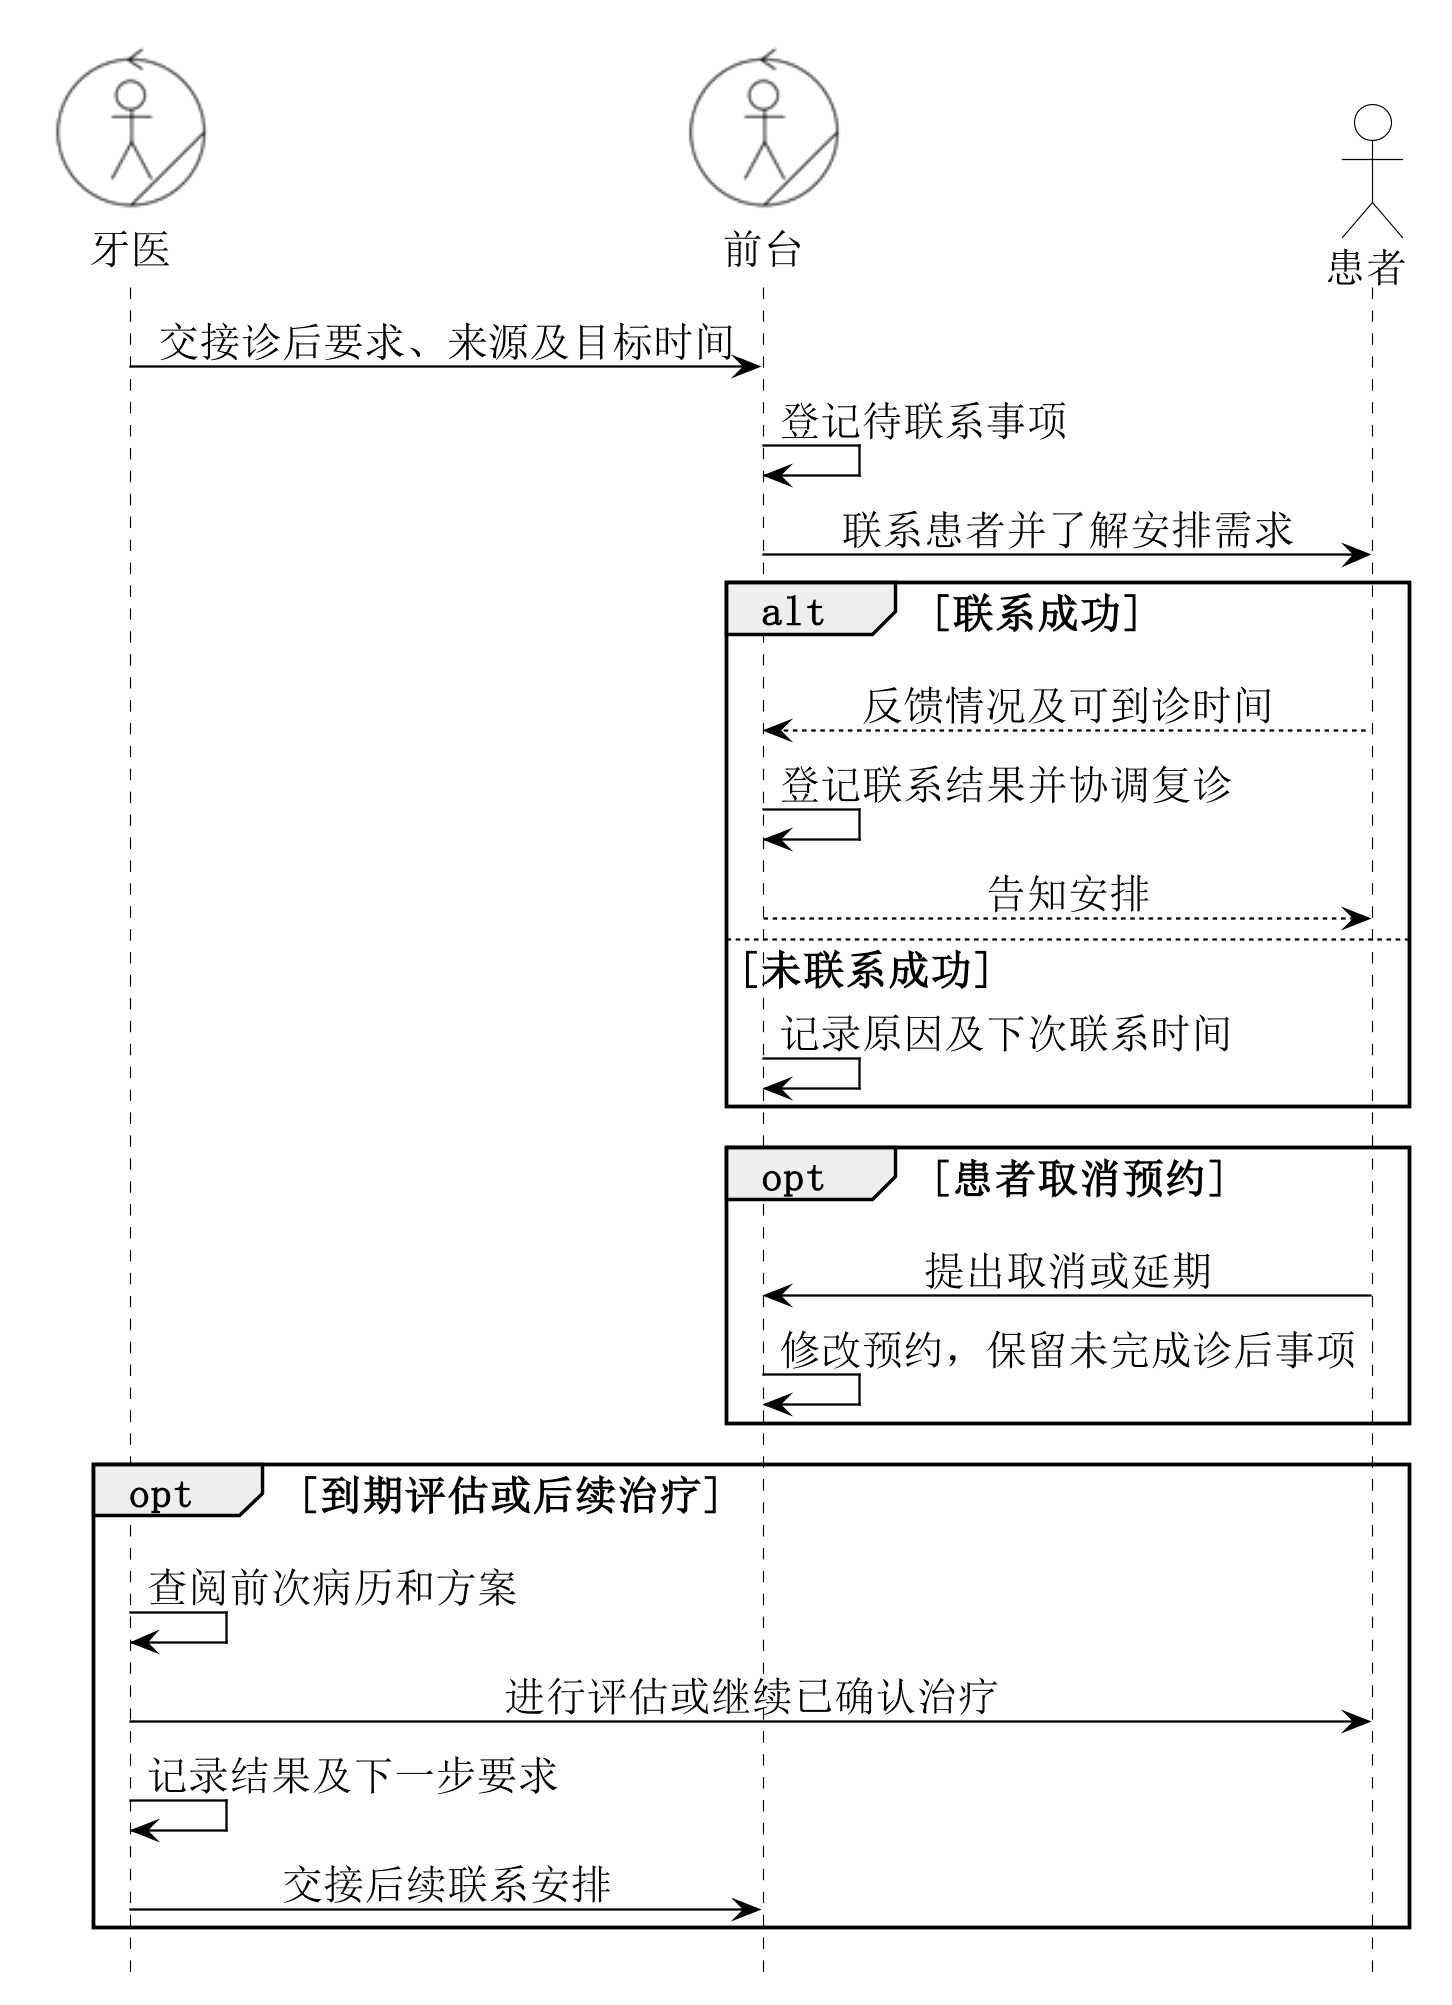
\includegraphics[width=\textwidth,height=18.5cm,keepaspectratio]{diagrams/02e-as-is-followup.png}
\caption{现状业务序列图：复诊与随访}
\label{fig:as-is-followup}
\end{figure}

复诊和随访都有明确的诊疗来源及办理结果；具体复诊时间和处理意见由牙医确定。

\clearpage
\subsubsection{接诊人员安排现状}

负责人结合牙医可出诊时间及诊所接诊能力拟定安排，与牙医确认后通知前台。前台据此受理预约；临时调整时，各岗位通过口头沟通及纸质记录同步变更。

\begin{figure}[!htbp]
\centering
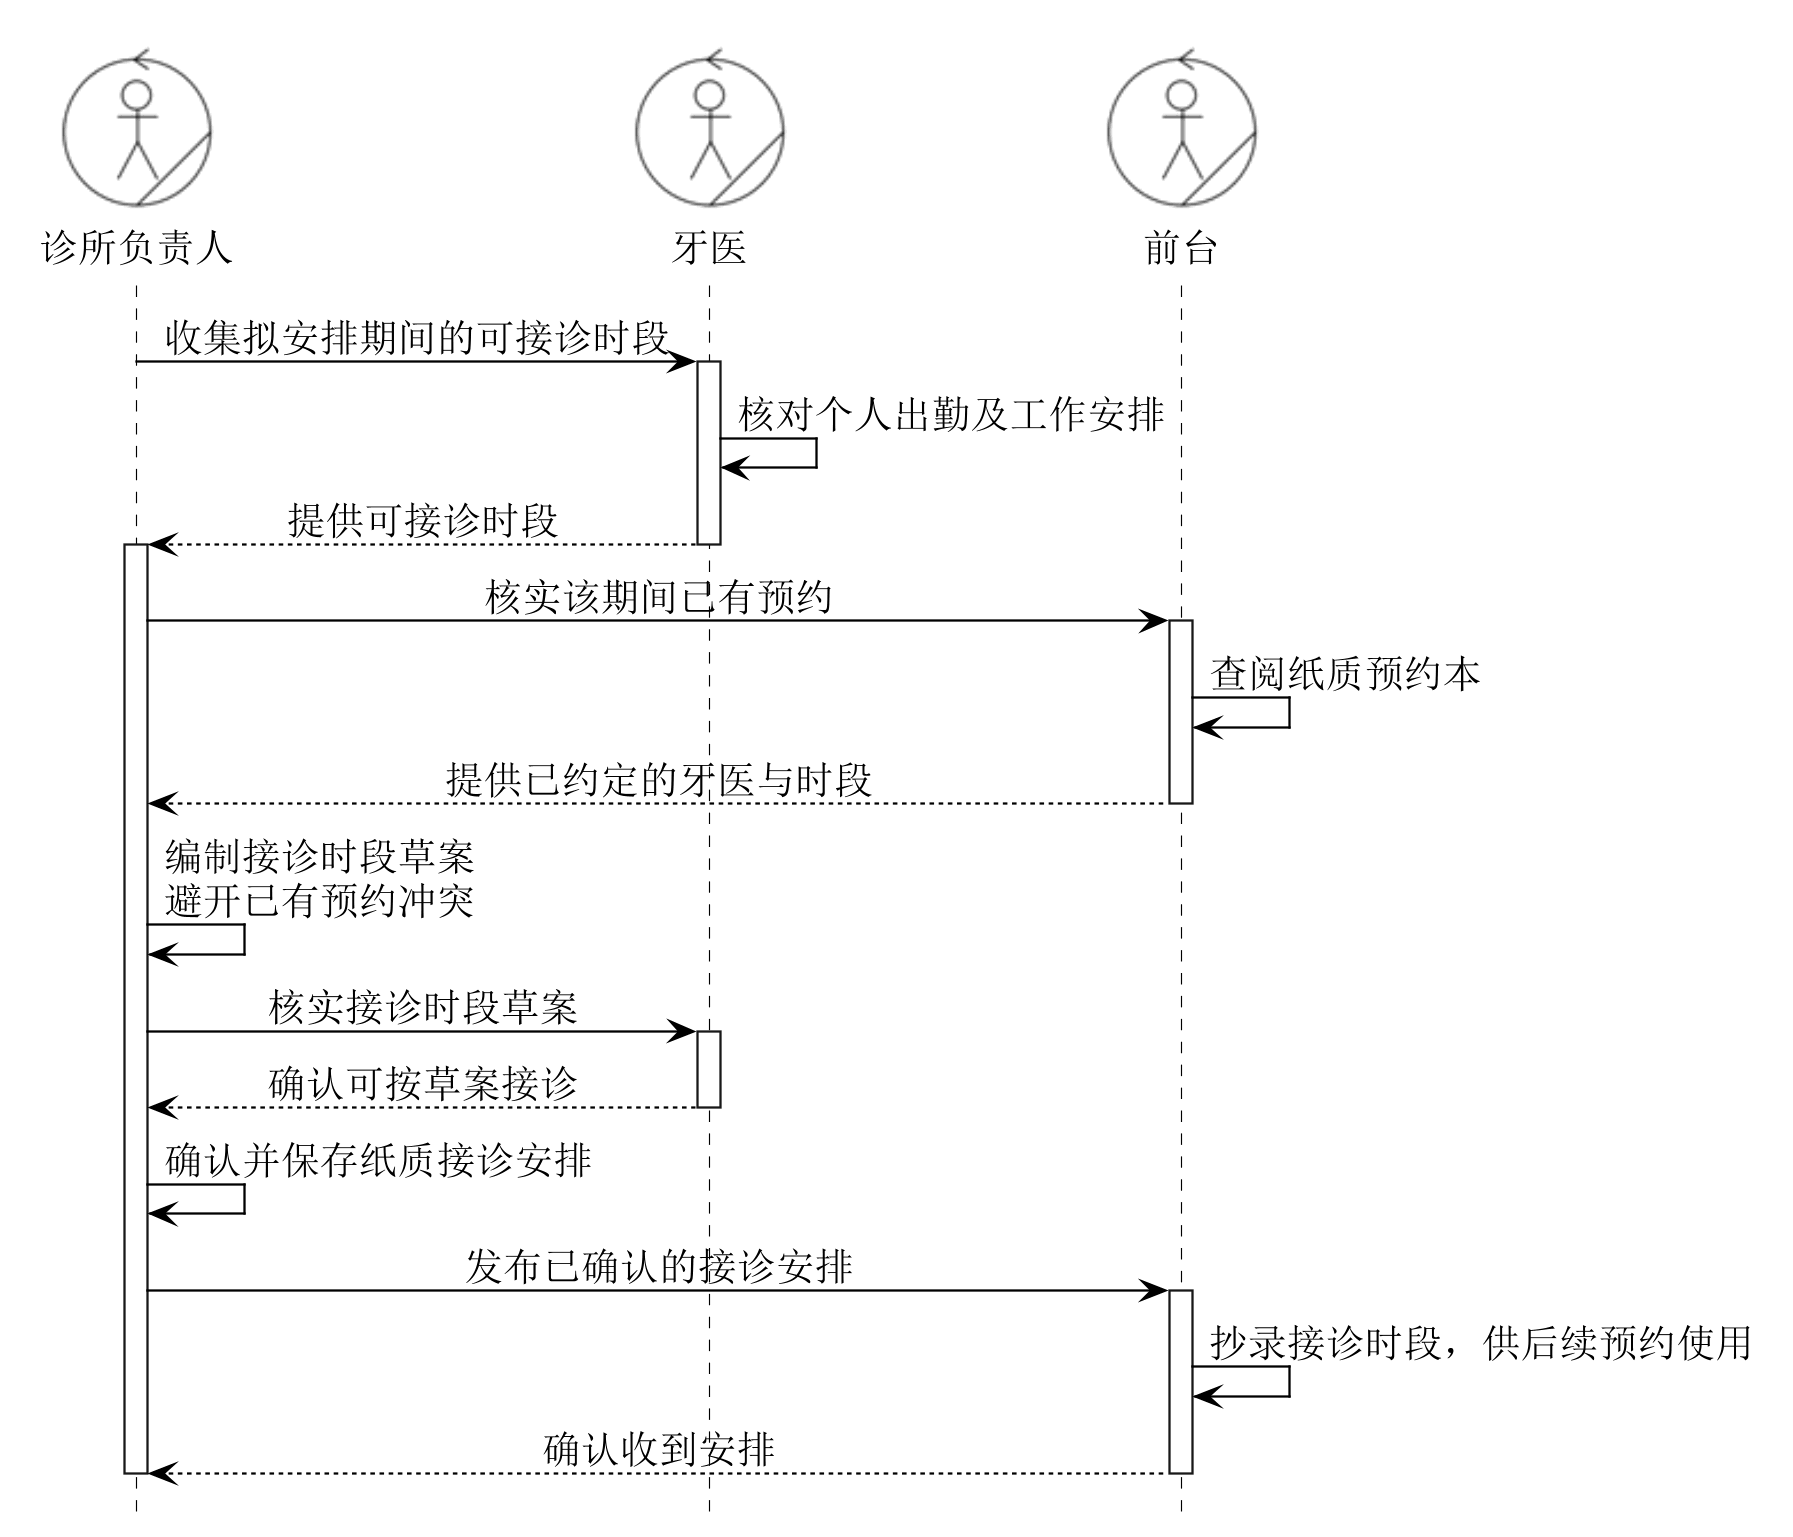
\includegraphics[width=\textwidth,height=13.4cm,keepaspectratio]{diagrams/02f-as-is-staffing.png}
\caption{现状业务序列图：接诊人员安排}
\label{fig:as-is-staffing}
\end{figure}

接诊安排支撑预约、现场接待和后续治疗；已有患者安排需要协调后才能变更。

\clearpage
\subsubsection{价目确认与维护现状}

负责人确认收费项目、价格及适用时间，交收费人员维护纸质价目表。收费人员核对并将变更告知牙医，保留旧价目以便核对既往费用。

\begin{figure}[!htbp]
\centering
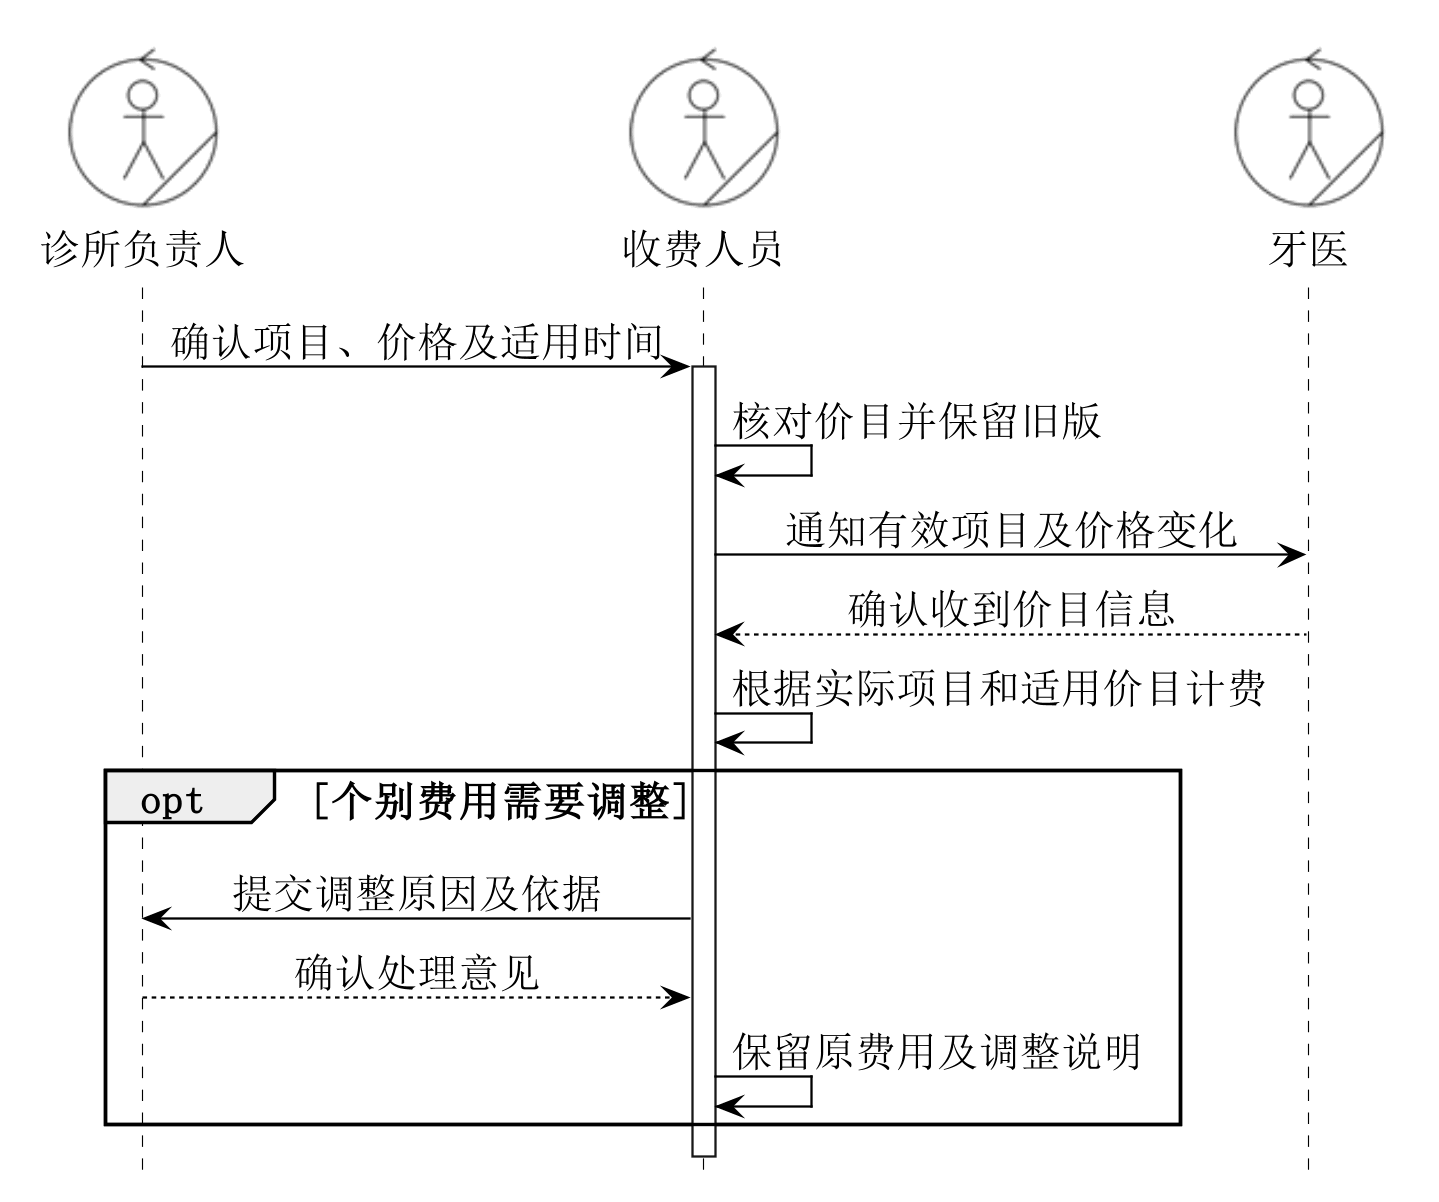
\includegraphics[width=\textwidth,height=13.4cm,keepaspectratio]{diagrams/02g-as-is-pricing.png}
\caption{现状业务序列图：价目确认与维护}
\label{fig:as-is-pricing}
\end{figure}

价目变更有明确确认责任和适用时间，项目价格能够一致使用并回查。

\clearpage
\subsubsection{材料入库、领用与盘点现状}

诊疗助理负责核对材料名称、单位及实际数量，用纸质台账分别记录入库、领用或盘点差异。需要补充材料或处理差异时，助理向负责人说明情况，由负责人确认处理。图中各分支是独立发生的办理场景。

\begin{figure}[!htbp]
\centering
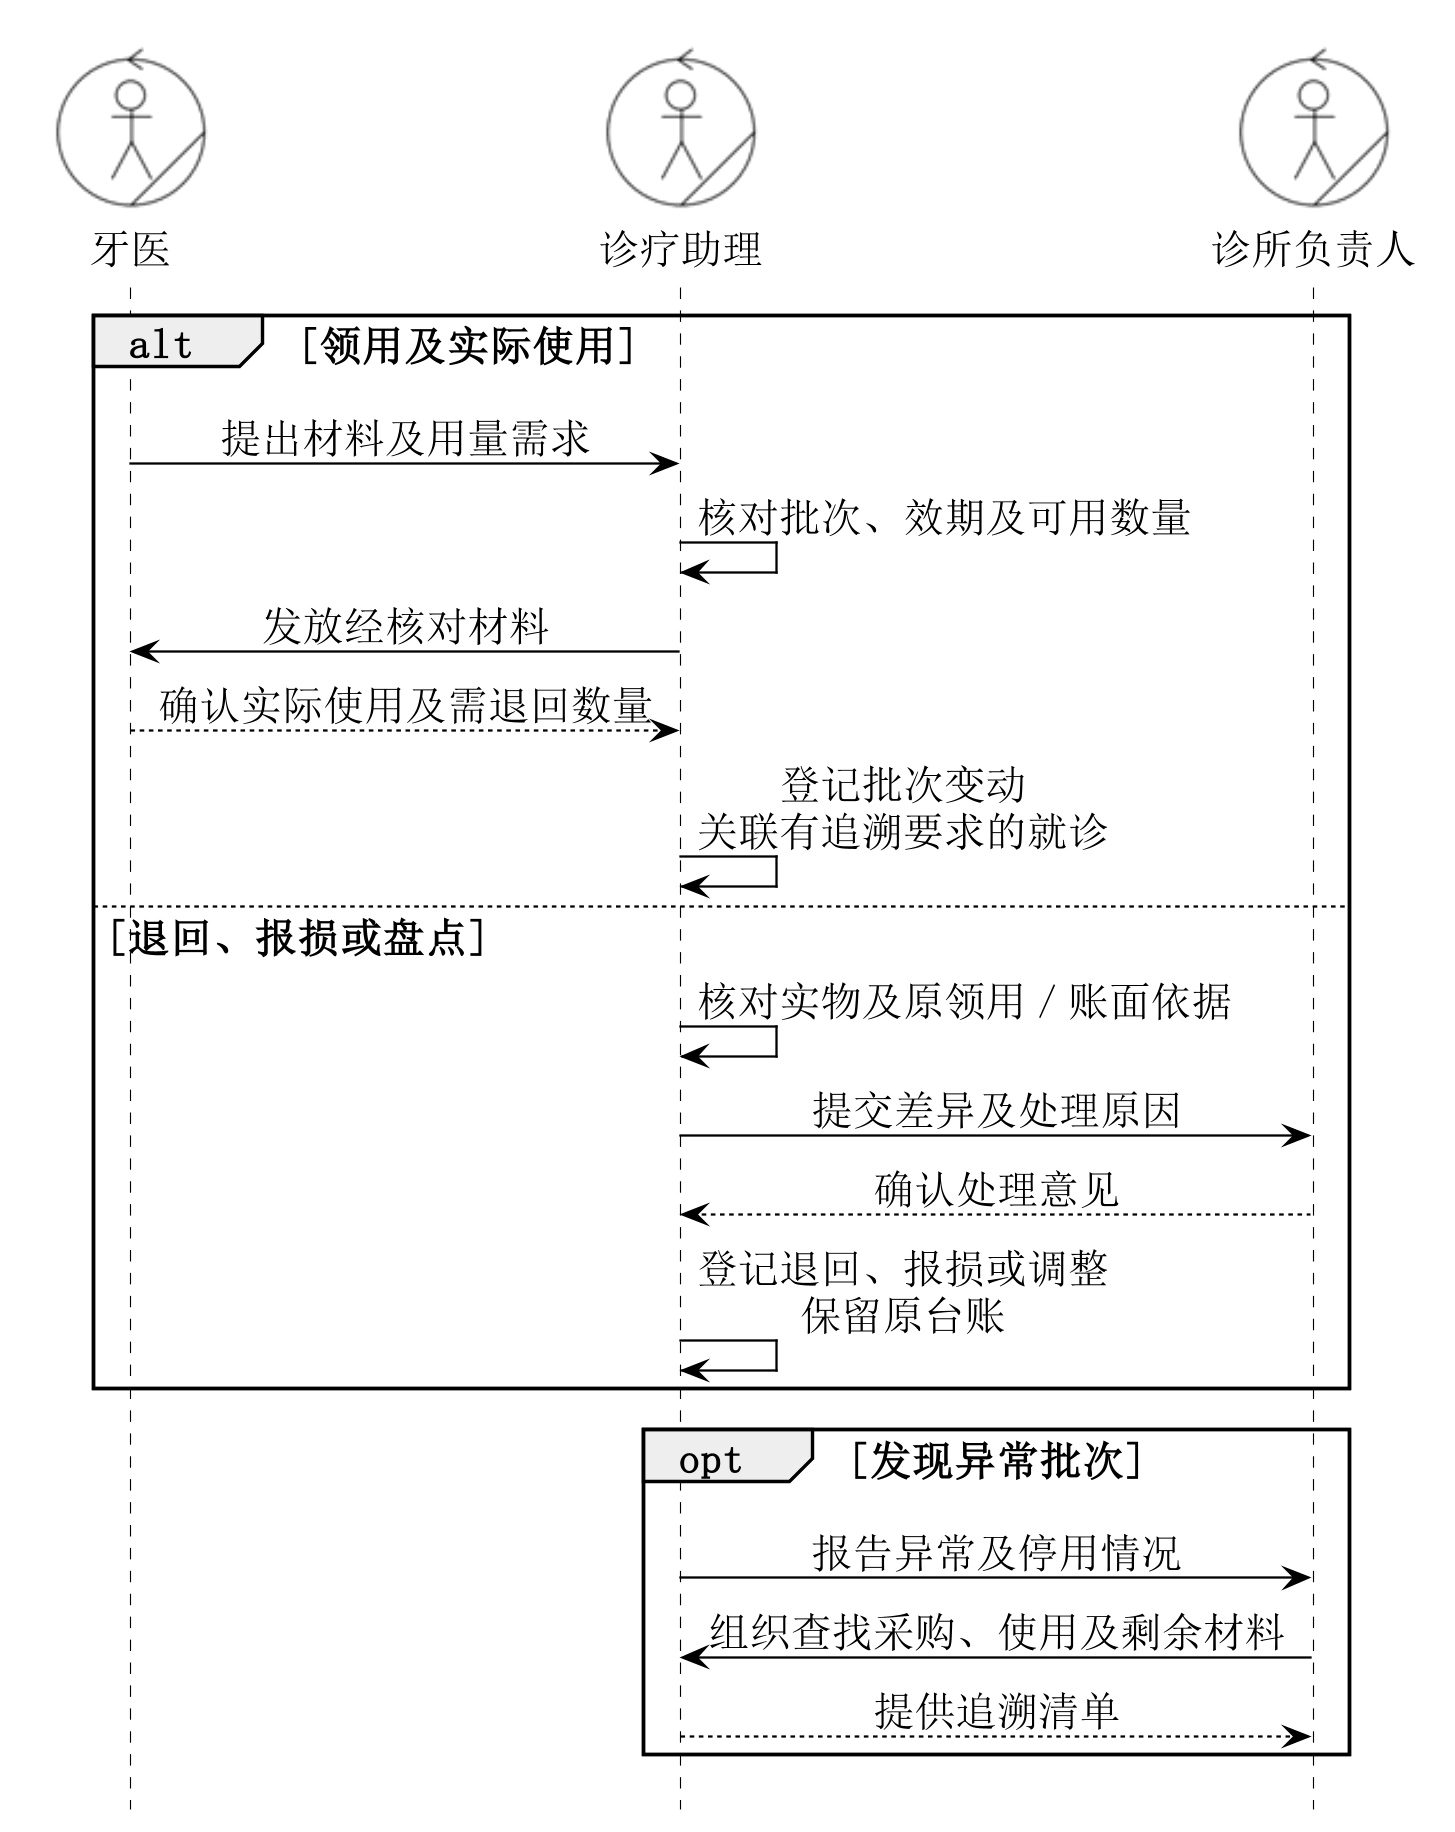
\includegraphics[width=\textwidth,height=18.0cm,keepaspectratio]{diagrams/02h-as-is-materials.png}
\caption{现状业务序列图：材料入库、领用与盘点}
\label{fig:as-is-materials}
\end{figure}

材料数量与实际收发保持对应，库存变化和差异处理可以追溯。

\clearpage
\subsubsection{日常业务与收款核对现状}

营业结束后，收费人员汇总收款登记和收据，核对实际款项；负责人查看接诊、诊疗及收款汇总。记录缺失或金额不一致时，相关岗位查阅原始单据并核实，完成更正后再确认当日结果。

\begin{figure}[!htbp]
\centering
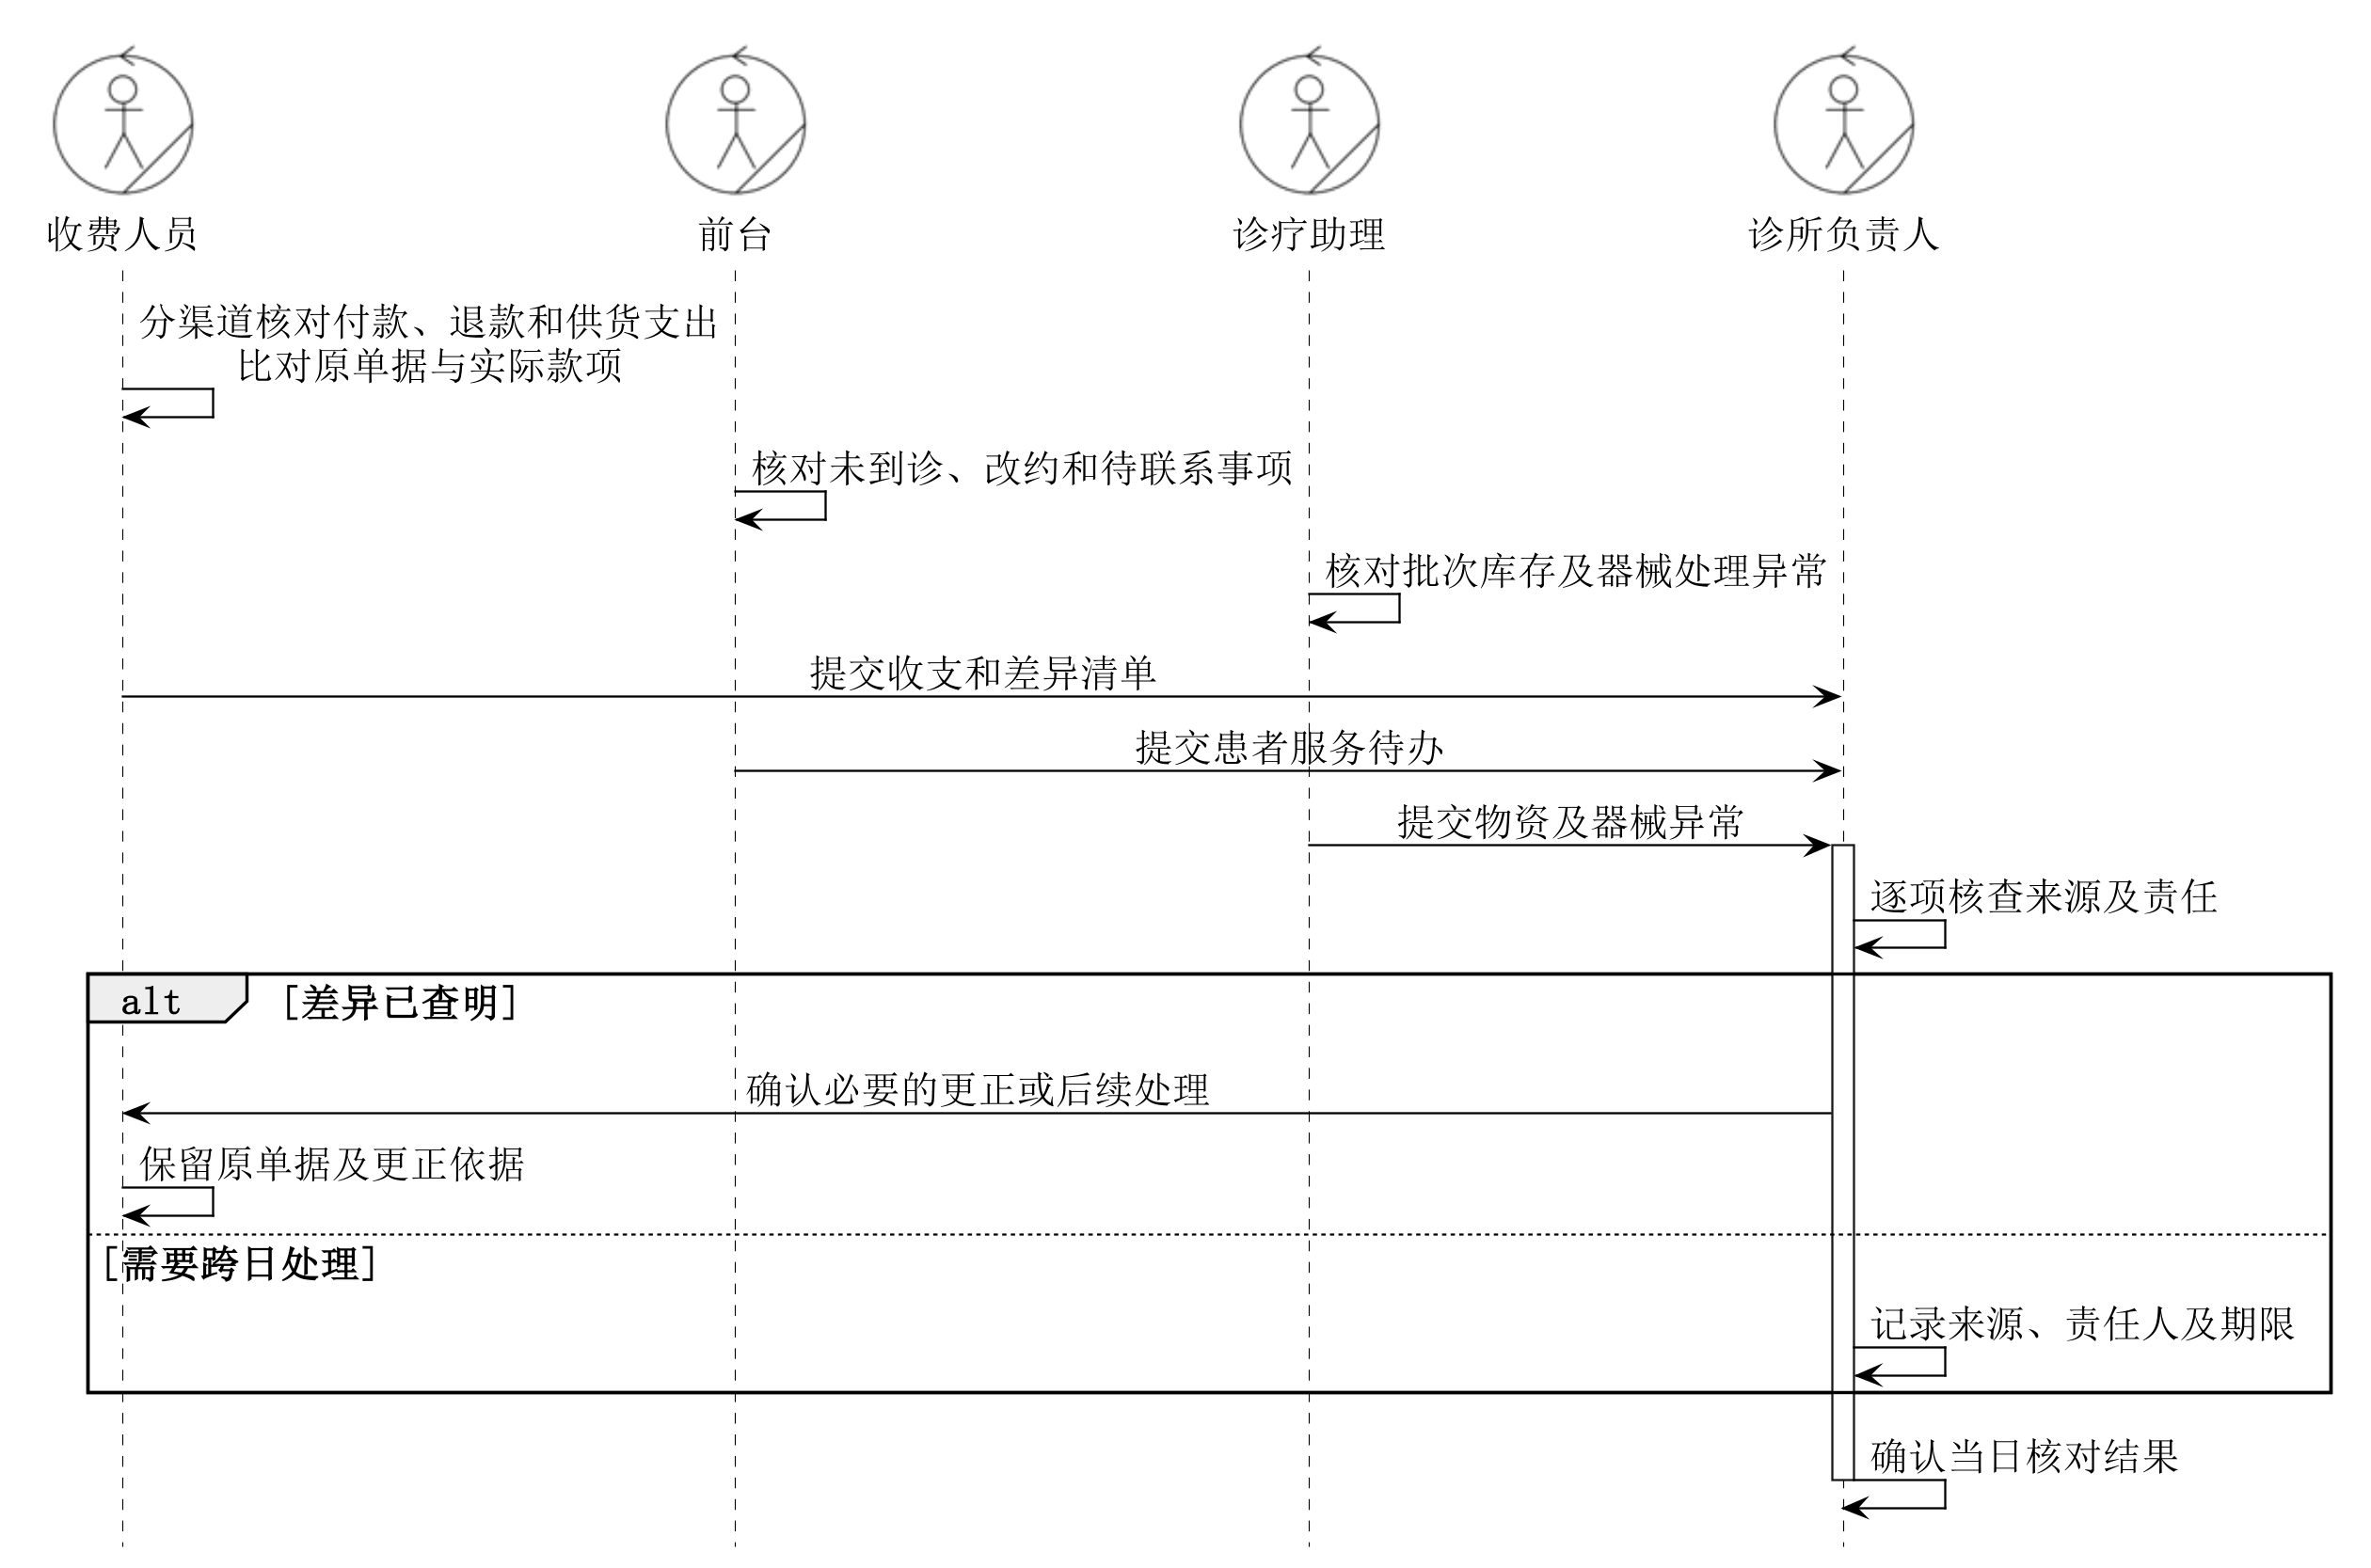
\includegraphics[width=\textwidth,height=14.0cm,keepaspectratio]{diagrams/02i-as-is-reconciliation.png}
\caption{现状业务序列图：日常业务与收款核对}
\label{fig:as-is-reconciliation}
\end{figure}

负责人获得与业务记录一致的运行情况；收款统计表示实际收入款项，不直接作为利润。

\clearpage
\subsection{改进业务序列图}

引入牙科诊所管理系统，统一保存预约、患者资料、诊疗、复诊、价目、材料及收款信息。各改进图与相应现状图采用同一业务场景；系统承担记录、查询、校验和汇总，相关岗位仍负责业务确认、临床判断、实物核对及实际收款。

\subsubsection{预约安排改进}

负责人已发布经牙医确认的接诊时段。前台先选定患者资料，再查询可用安排并与患者协商；时段内预约沿用其牙医确认依据，需要调整时先核实并更新接诊安排。系统检查时段及冲突，保存患者与预约的关联并返回确认结果。预约变更同步更新可用安排，前台负责向患者告知结果。

\begin{figure}[!htbp]
\centering
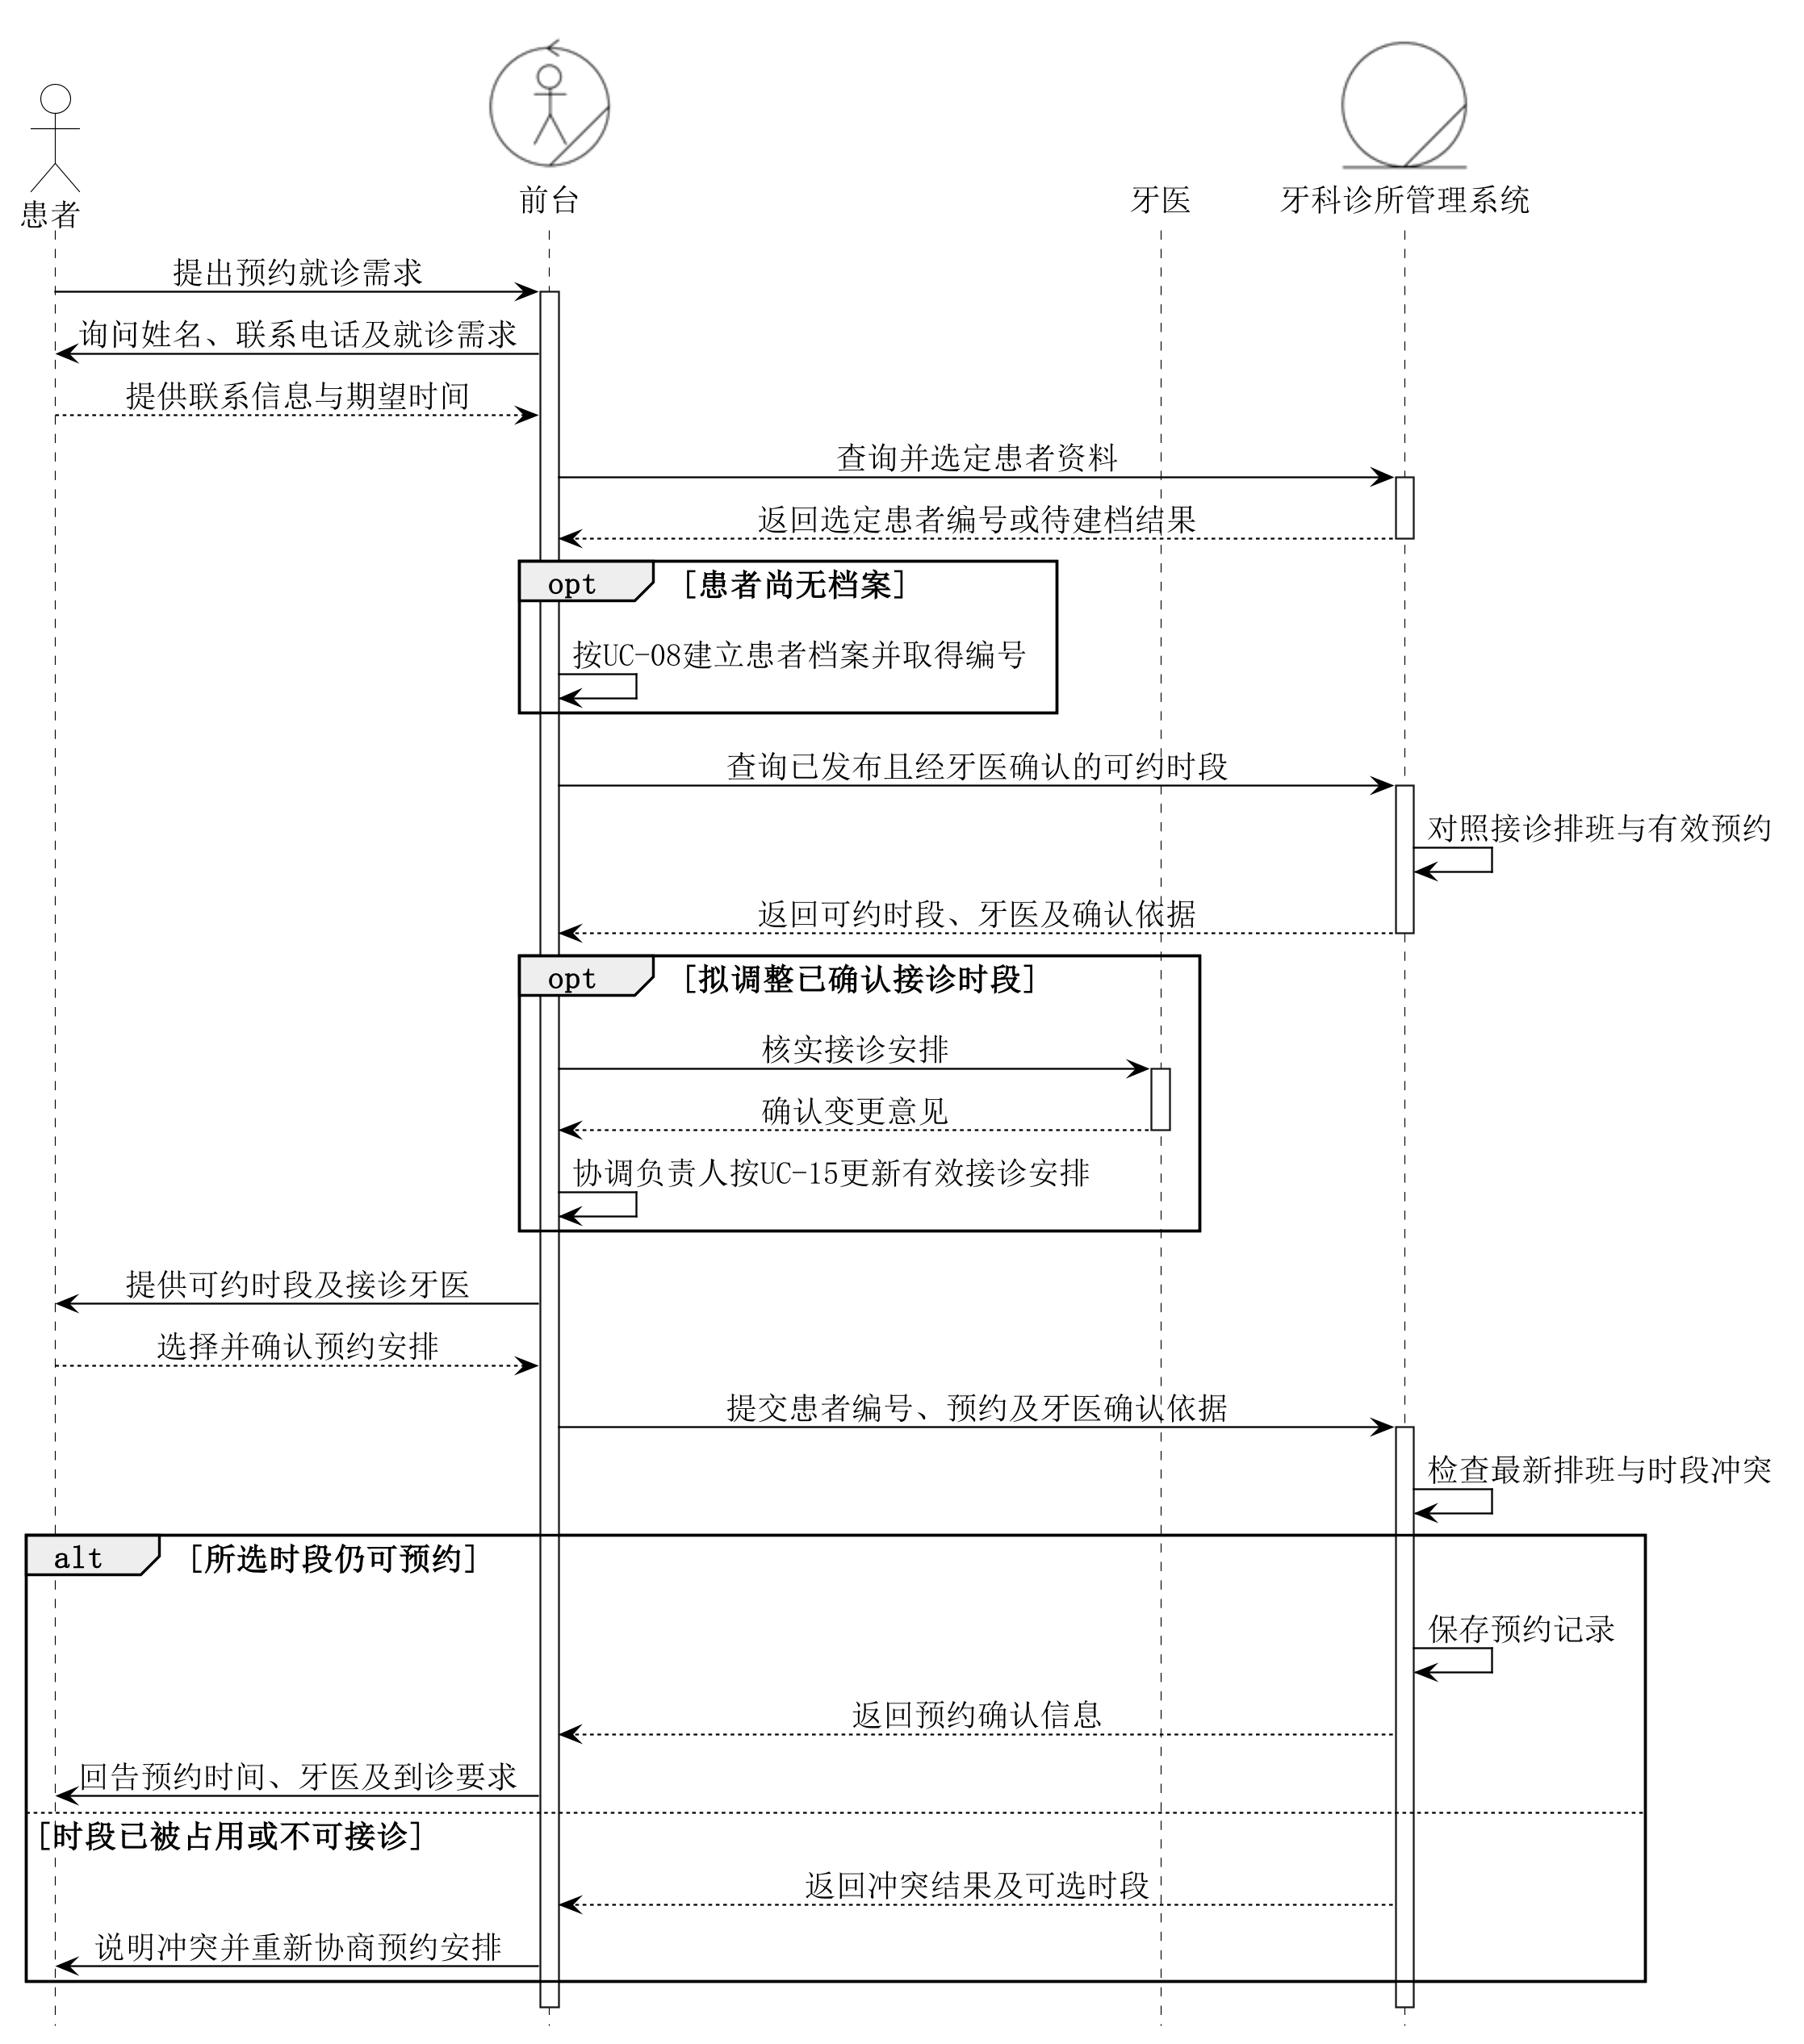
\includegraphics[width=\textwidth,height=13.8cm,keepaspectratio]{diagrams/03c-to-be-appointment.png}
\caption{改进业务序列图：预约安排}
\label{fig:to-be-appointment}
\end{figure}

患者获得明确的就诊时间与接诊安排，前台保留后续接待所需的预约依据。

\clearpage
\subsubsection{到诊接待改进}

已预约患者按约到诊，前台查询预约及已确认接诊安排，核对患者身份后登记到诊。系统关联已有预约和患者资料，返回本次就诊信息；前台告知候诊安排。实际安排与记录不符时，由相关人员先核实并更新。

\begin{figure}[!htbp]
\centering
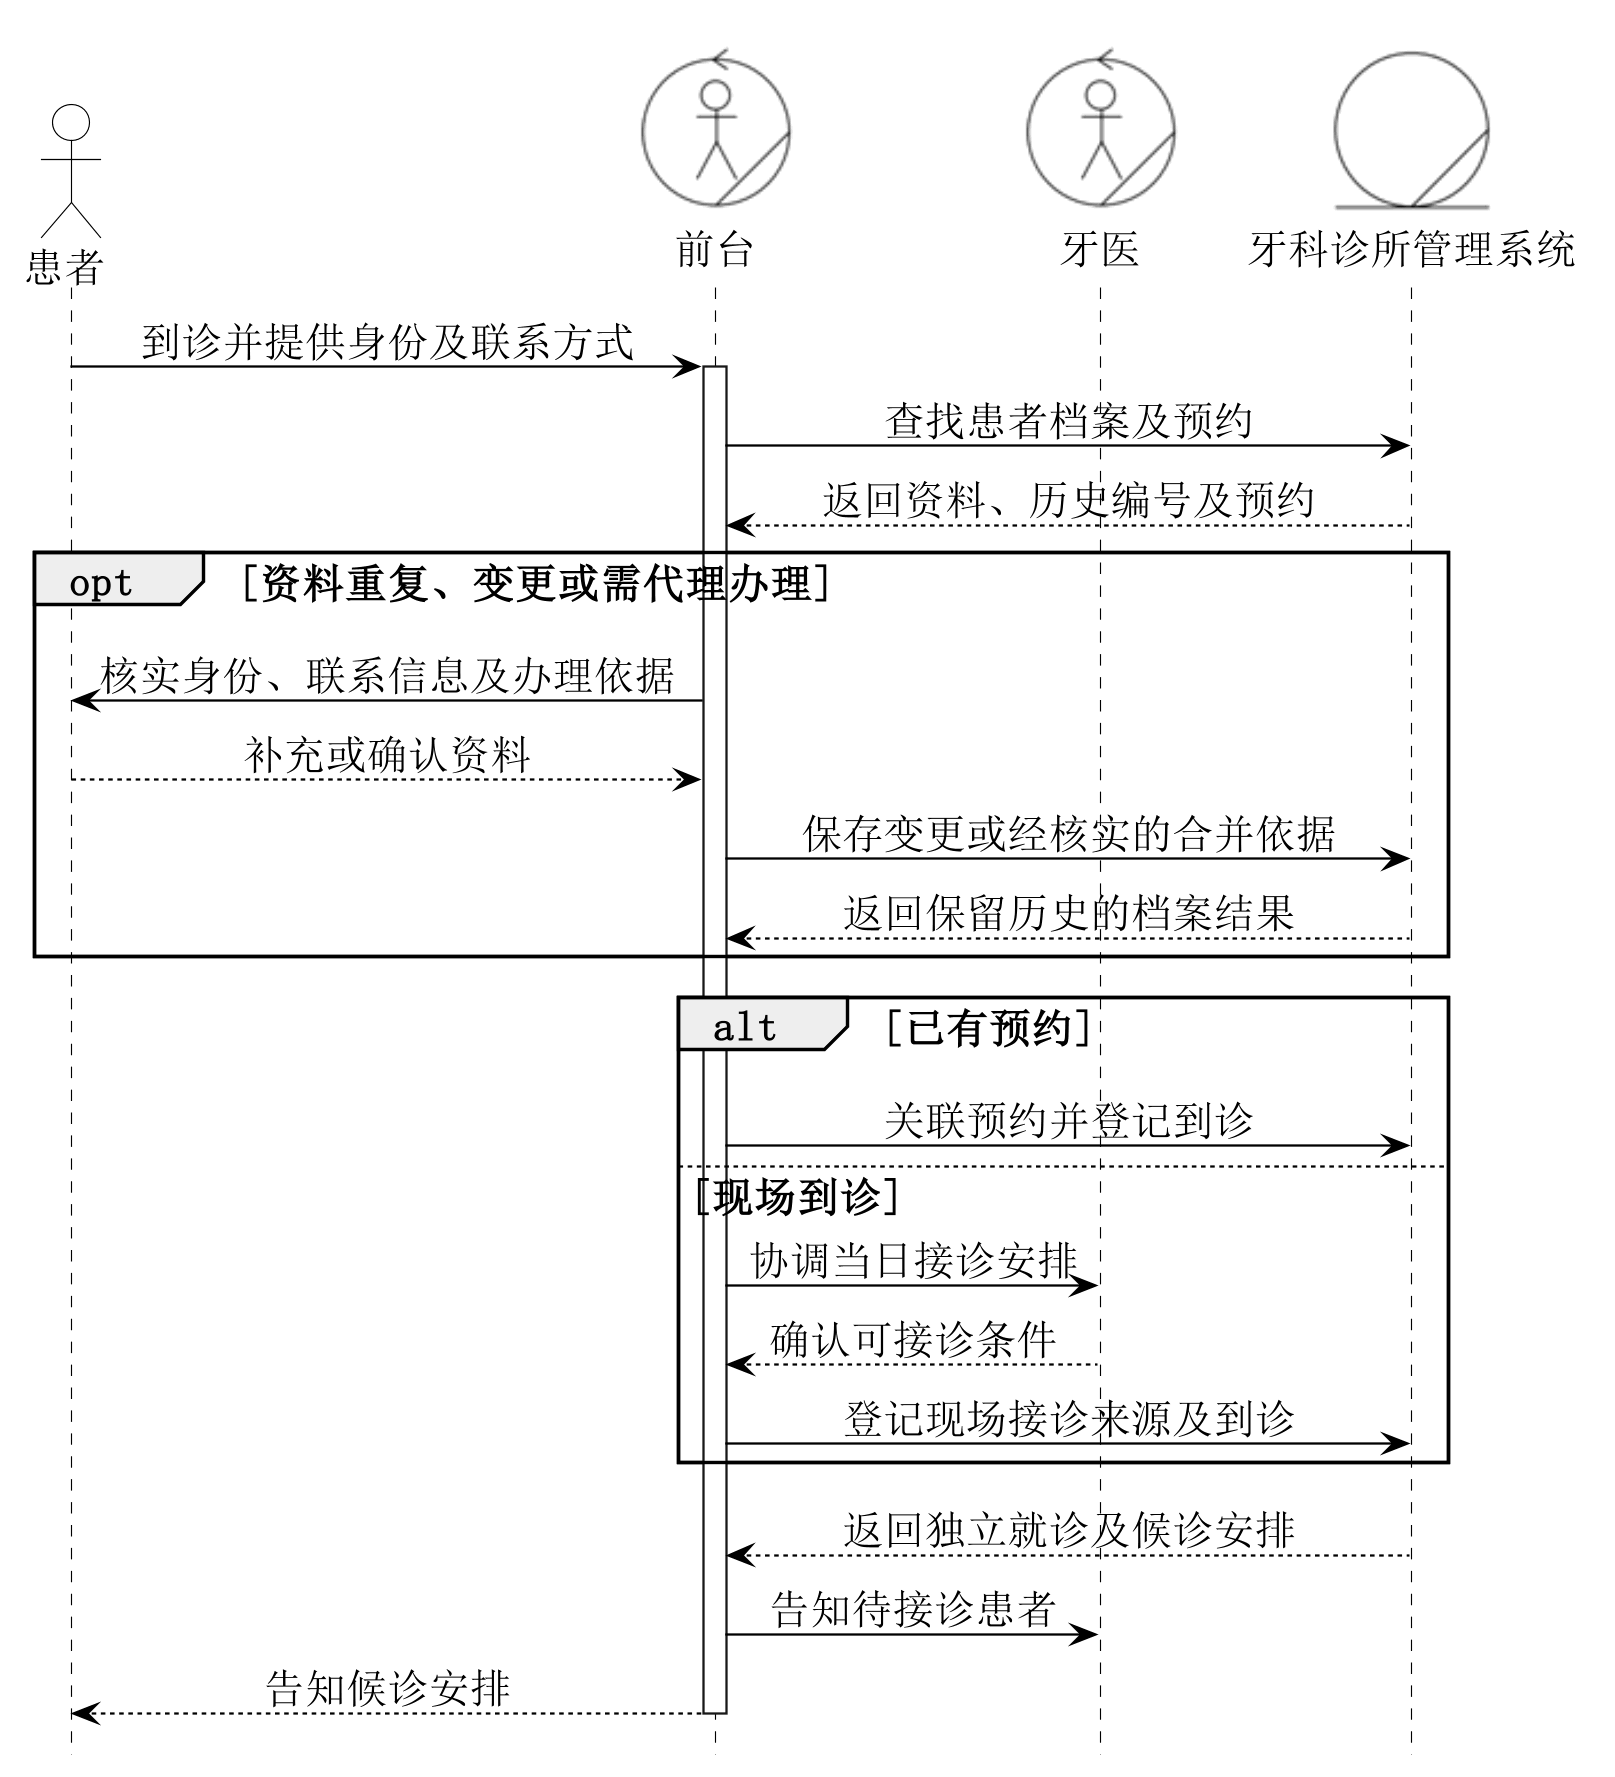
\includegraphics[width=\textwidth,height=11.3cm,keepaspectratio]{diagrams/03-to-be-business-sequence.png}
\caption{改进业务序列图：到诊接待}
\label{fig:to-be-reception}
\end{figure}

图中a为开始核对身份与预约的时点，b为到诊登记和候诊告知完成的时点，对应愿景中的接待办理时长。

\clearpage
\subsubsection{检查诊断与治疗改进}

牙医查阅本次就诊与既往诊疗记录，补充病史、牙位和检查所见，记录诊断与方案。牙医向患者说明方案并取得确认后，助理完成诊疗准备，牙医实施治疗，保存治疗经过、实际完成项目及诊后与复诊要求。系统保持这些记录与患者及本次就诊的关联，供后续收费和复诊使用。

\begin{figure}[!htbp]
\centering
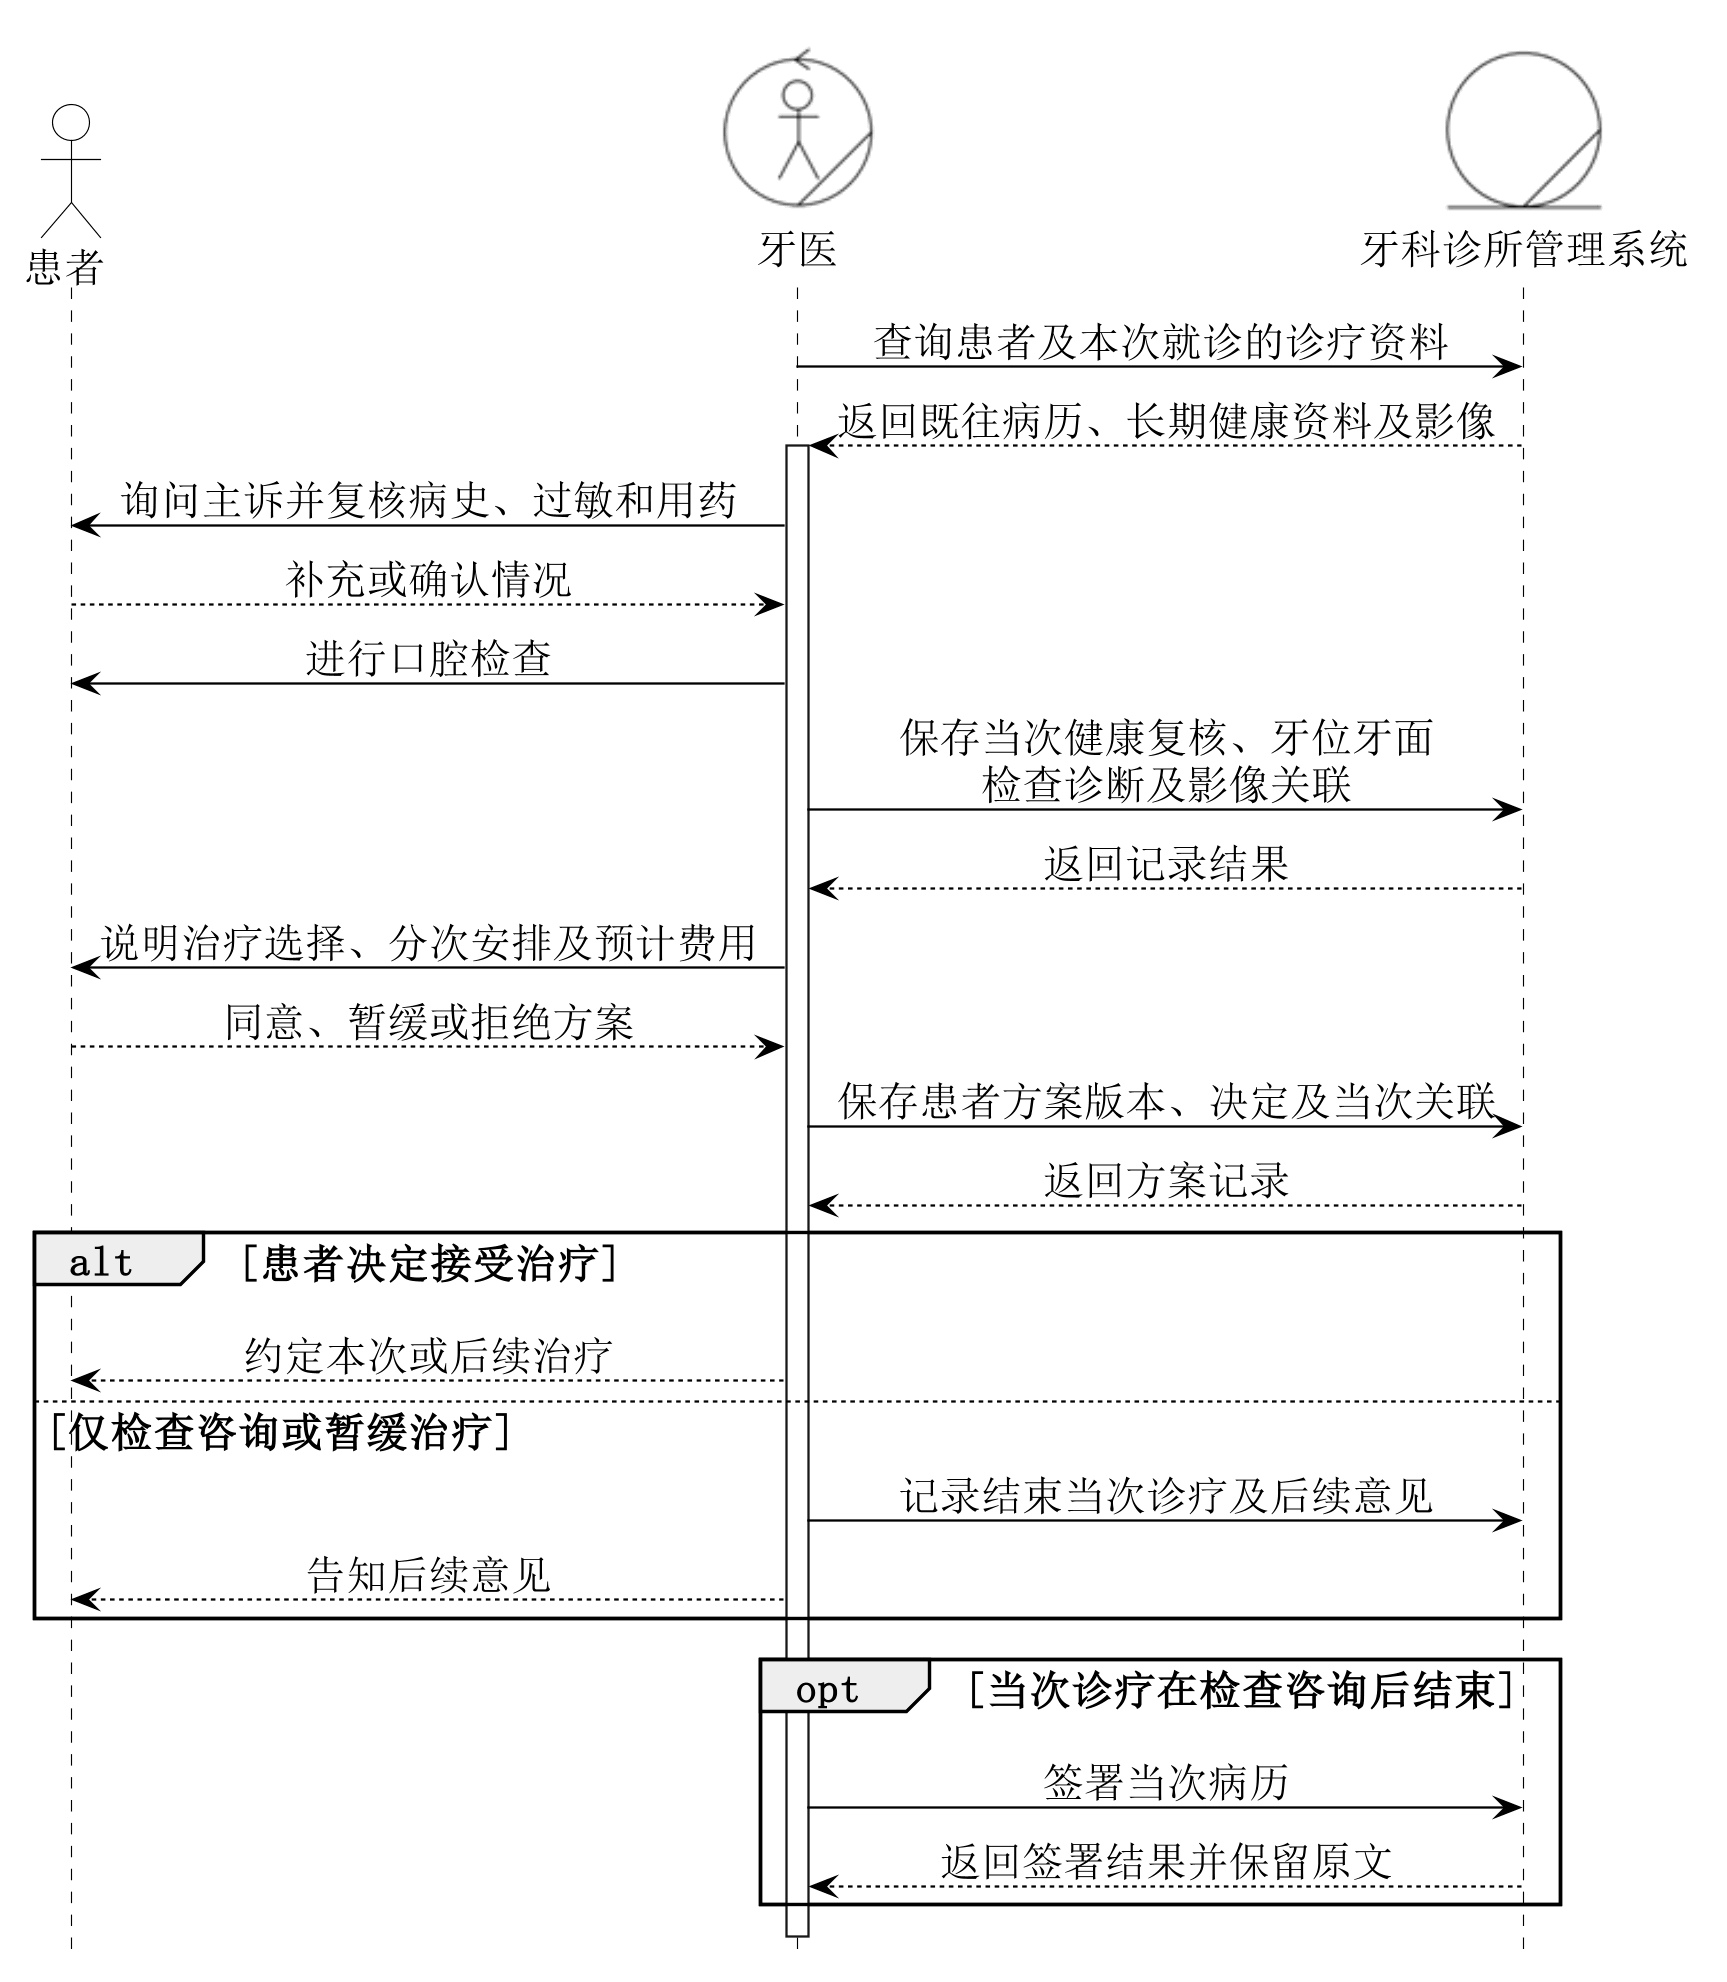
\includegraphics[width=\textwidth,height=15.5cm,keepaspectratio]{diagrams/03d-to-be-clinical.png}
\caption{改进业务序列图：检查诊断与治疗}
\label{fig:to-be-clinical}
\end{figure}

牙医承担检查诊断、方案沟通和治疗责任；助理承担准备与协助责任。治疗记录反映实际发生的诊疗，不以收费项目清单代替病历。

\clearpage
\subsubsection{费用结算改进}

牙医已确认本次实际完成项目及数量，适用价目已维护。收费人员查询待结算明细，与患者核对费用并清点现金，再登记实收金额；系统计算应收和找零，保存结算结果并提供收据。项目未确认、价格缺失或费用有异议时，应先交相关人员核实。

\begin{figure}[!htbp]
\centering
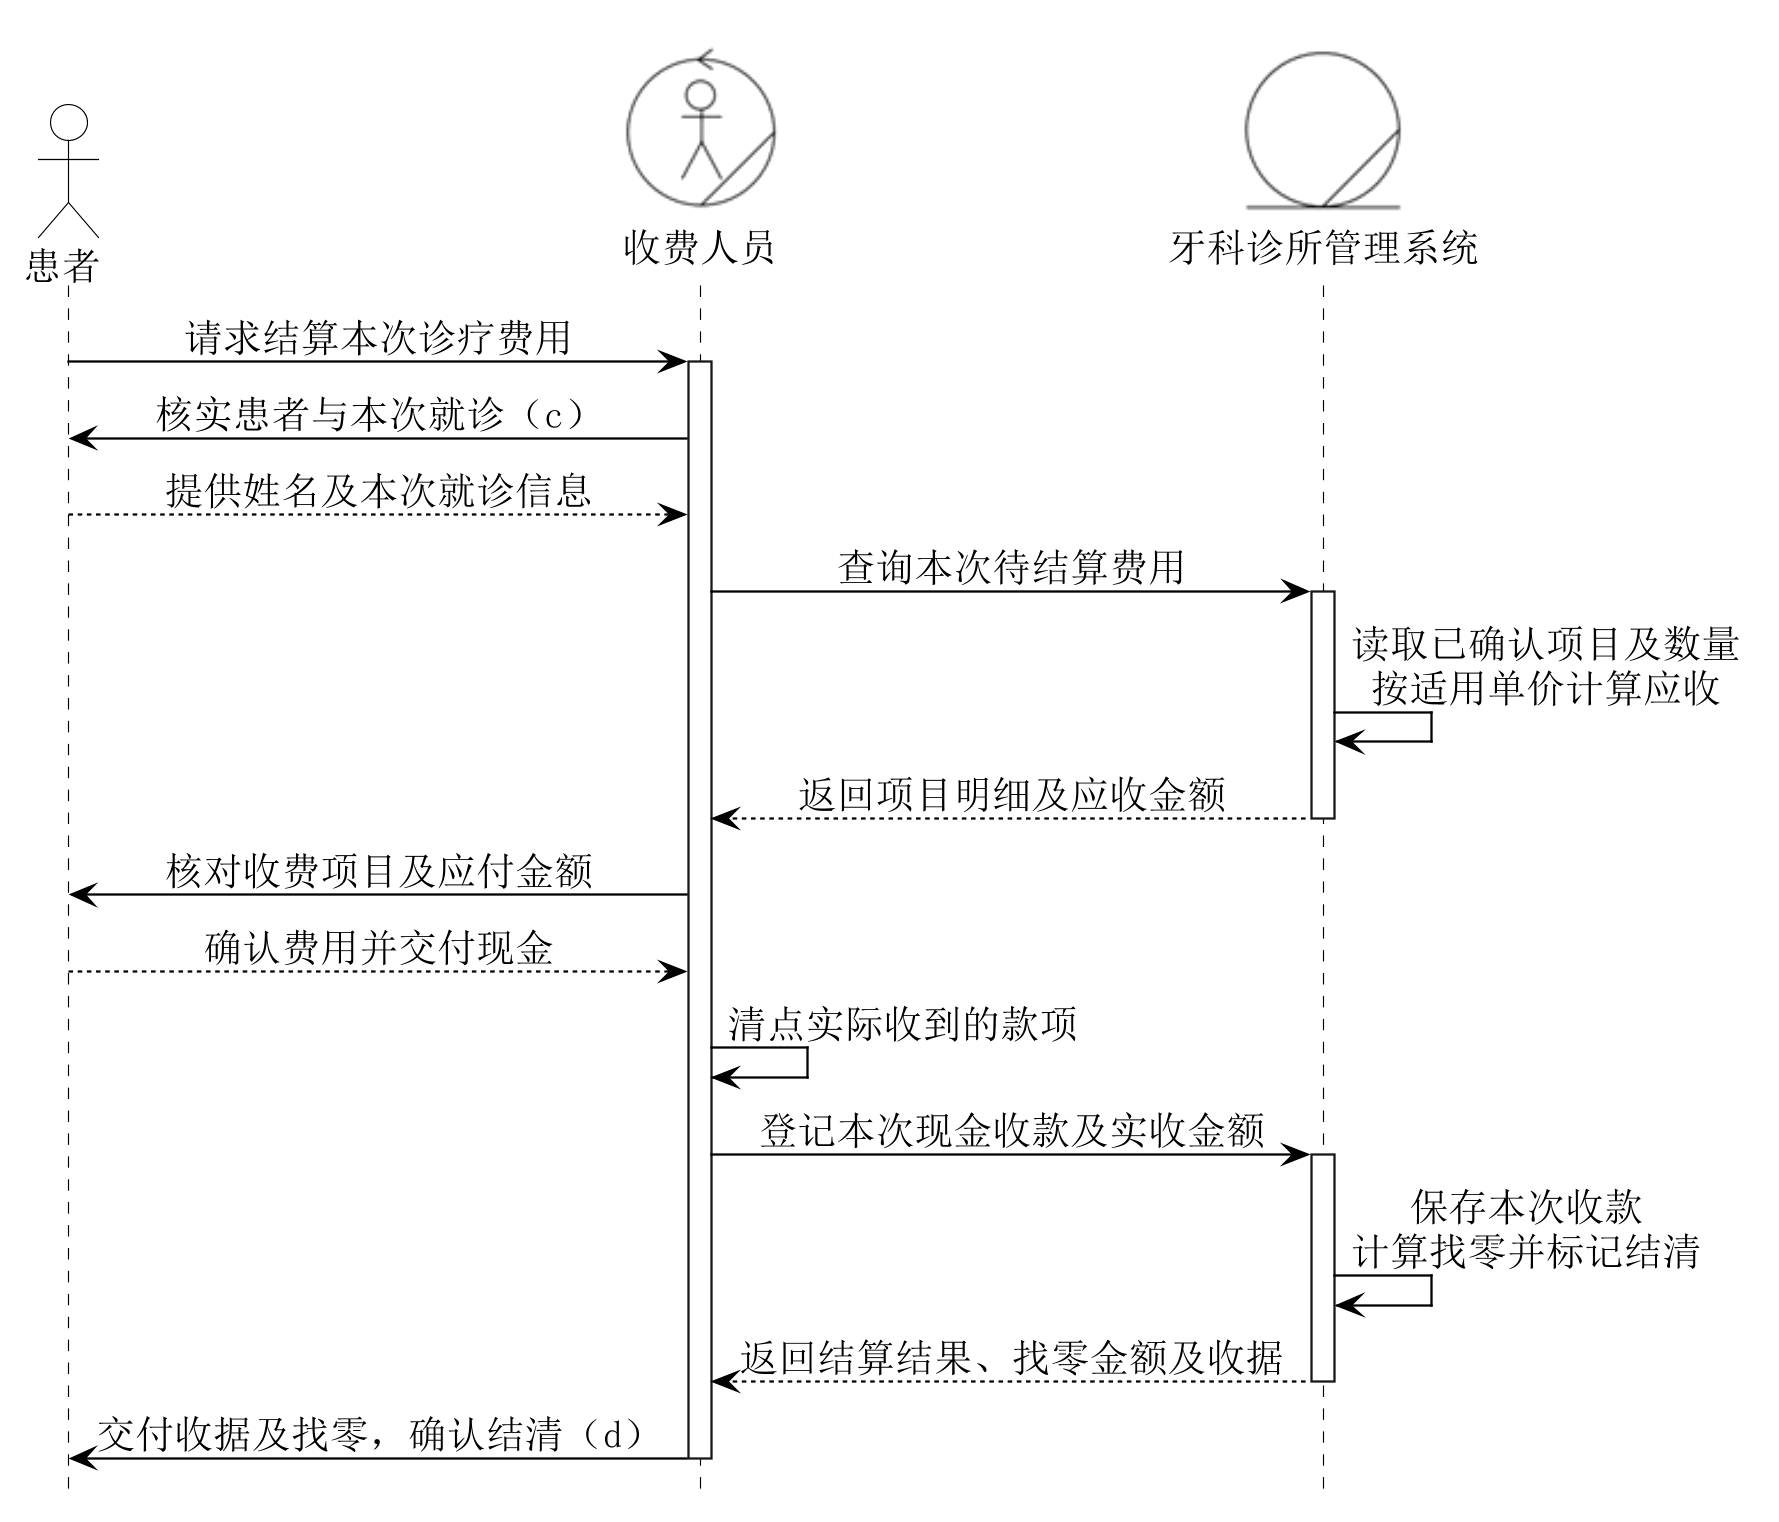
\includegraphics[width=\textwidth,height=13.0cm,keepaspectratio]{diagrams/03b-to-be-billing-sequence.png}
\caption{改进业务序列图：费用结算}
\label{fig:to-be-billing}
\end{figure}

图中c为开始核对本次患者与诊疗费用的时点，d为收款登记、凭据及找零交付完成的时点，对应愿景中的结算办理时长。

\clearpage
\subsubsection{复诊与随访改进}

牙医记录复诊或随访要求并关联前次就诊。前台查询待联系事项，联系患者并登记结果，需要到诊时按可接诊时段办理预约。复诊牙医查阅关联记录，评估本次情况并保存处理结果；未联系成功或患者需调整时间时，前台保留原因及后续安排。

\begin{figure}[!htbp]
\centering
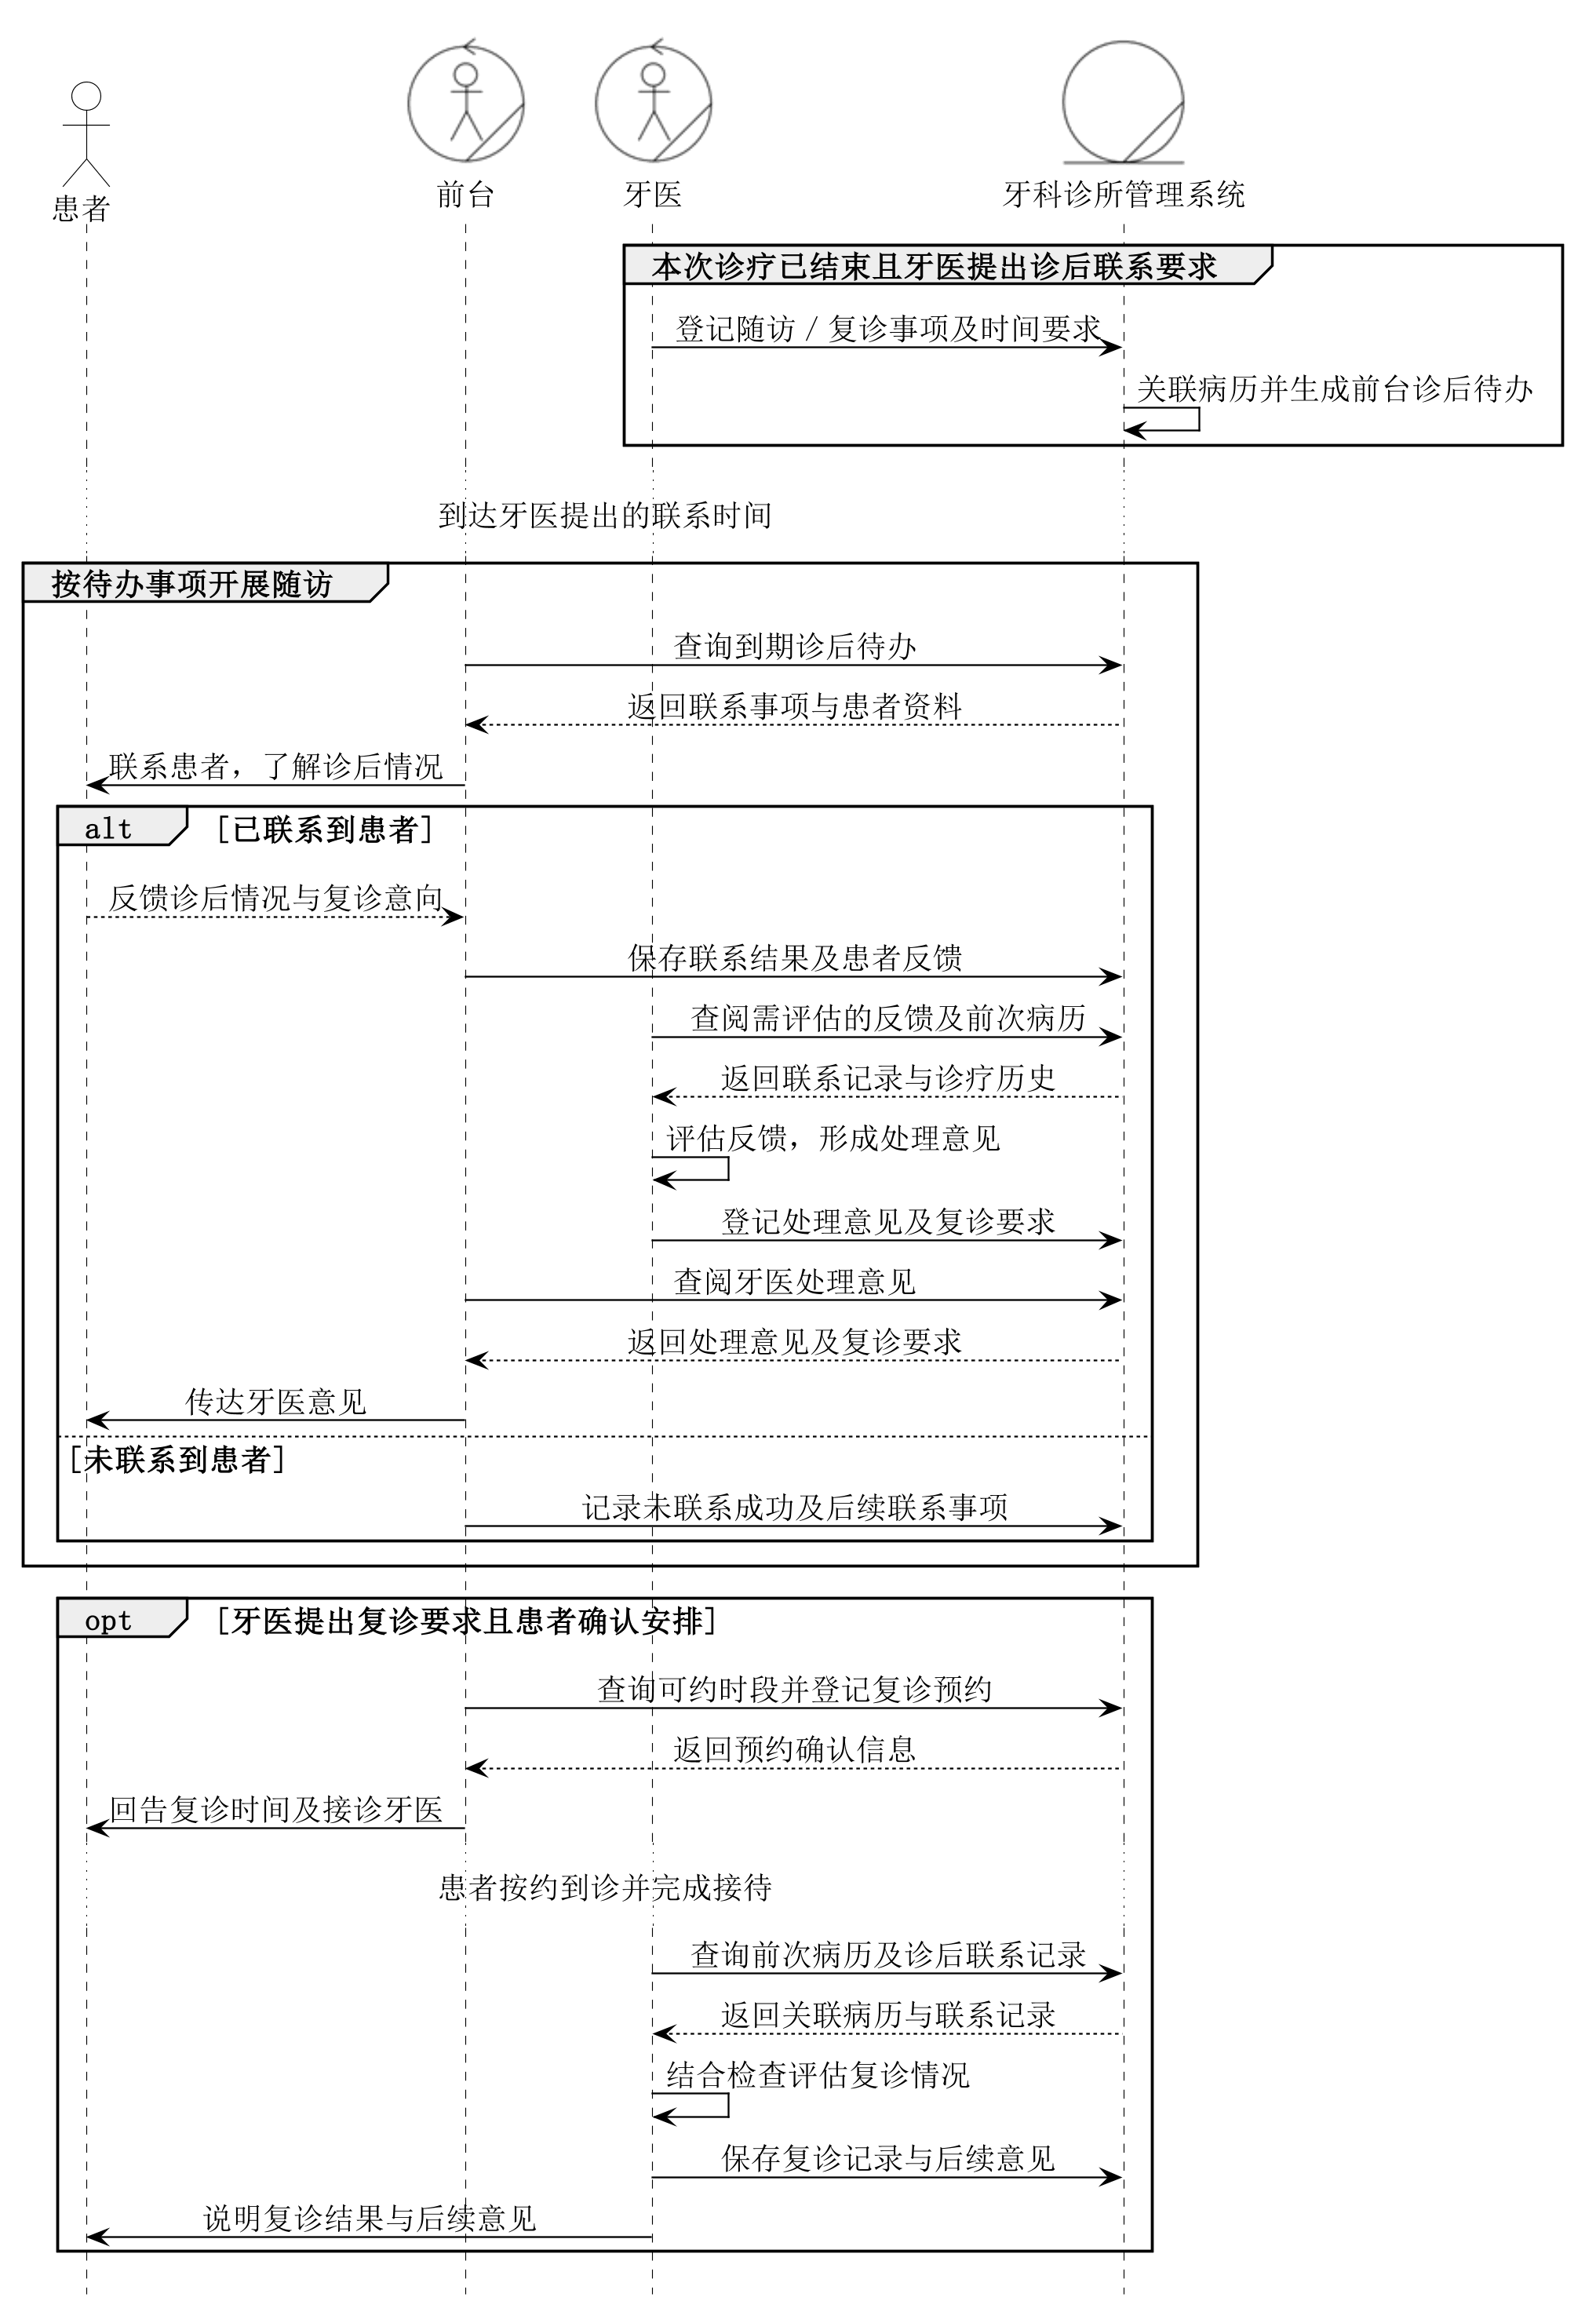
\includegraphics[width=\textwidth,height=18.5cm,keepaspectratio]{diagrams/03e-to-be-followup.png}
\caption{改进业务序列图：复诊与随访}
\label{fig:to-be-followup}
\end{figure}

复诊和随访都有明确的诊疗来源及办理结果；具体复诊时间和处理意见由牙医确定。

\clearpage
\subsubsection{接诊人员安排改进}

负责人汇总牙医可出诊时间并确认接诊时段，在系统中发布安排。系统检查时段，提示已有预约与新安排的冲突；负责人协调处理后确认变更，前台与牙医查询同一份有效安排。

\begin{figure}[!htbp]
\centering
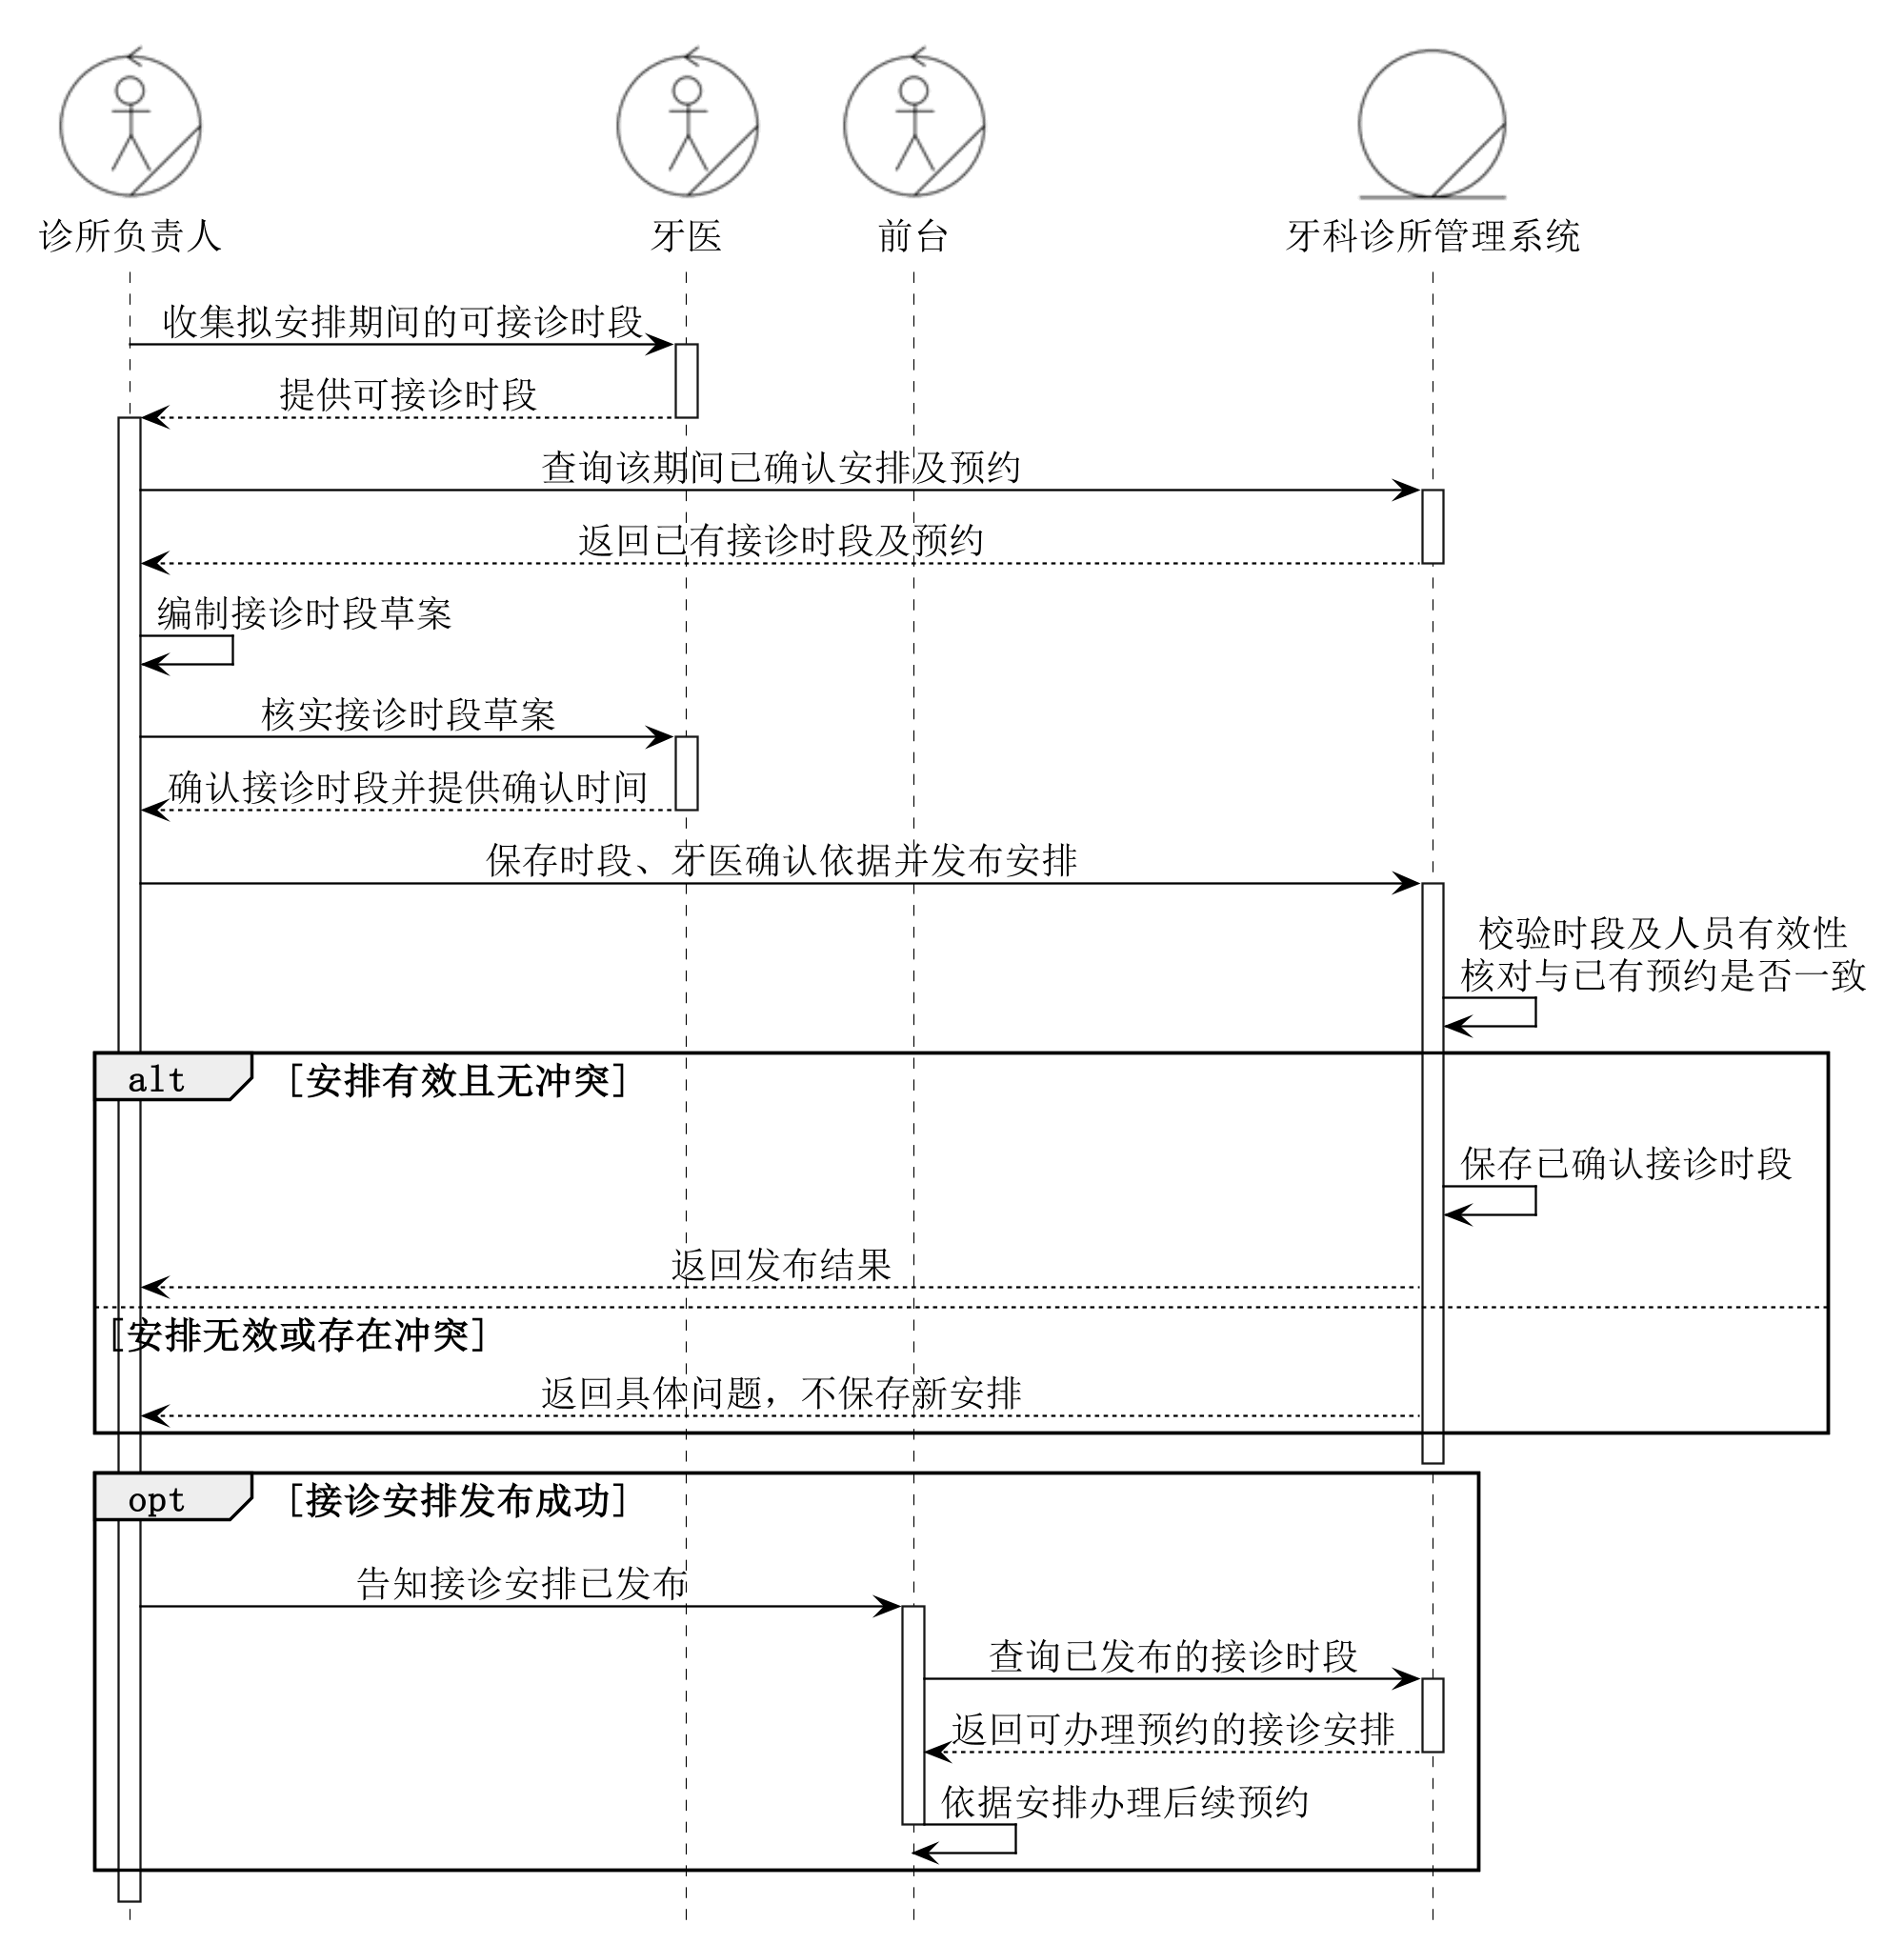
\includegraphics[width=\textwidth,height=13.4cm,keepaspectratio]{diagrams/03f-to-be-staffing.png}
\caption{改进业务序列图：接诊人员安排}
\label{fig:to-be-staffing}
\end{figure}

接诊安排支撑预约、现场接待和后续治疗；已有患者安排需要协调后才能变更。

\clearpage
\subsubsection{价目确认与维护改进}

负责人先确认收费项目、价格及适用时间，收费人员依据确认结果录入价目。系统检查价目完整性及区间重叠，保存有效版本，供治疗前费用说明和结算使用；既往费用仍保留原单价依据。

\begin{figure}[!htbp]
\centering
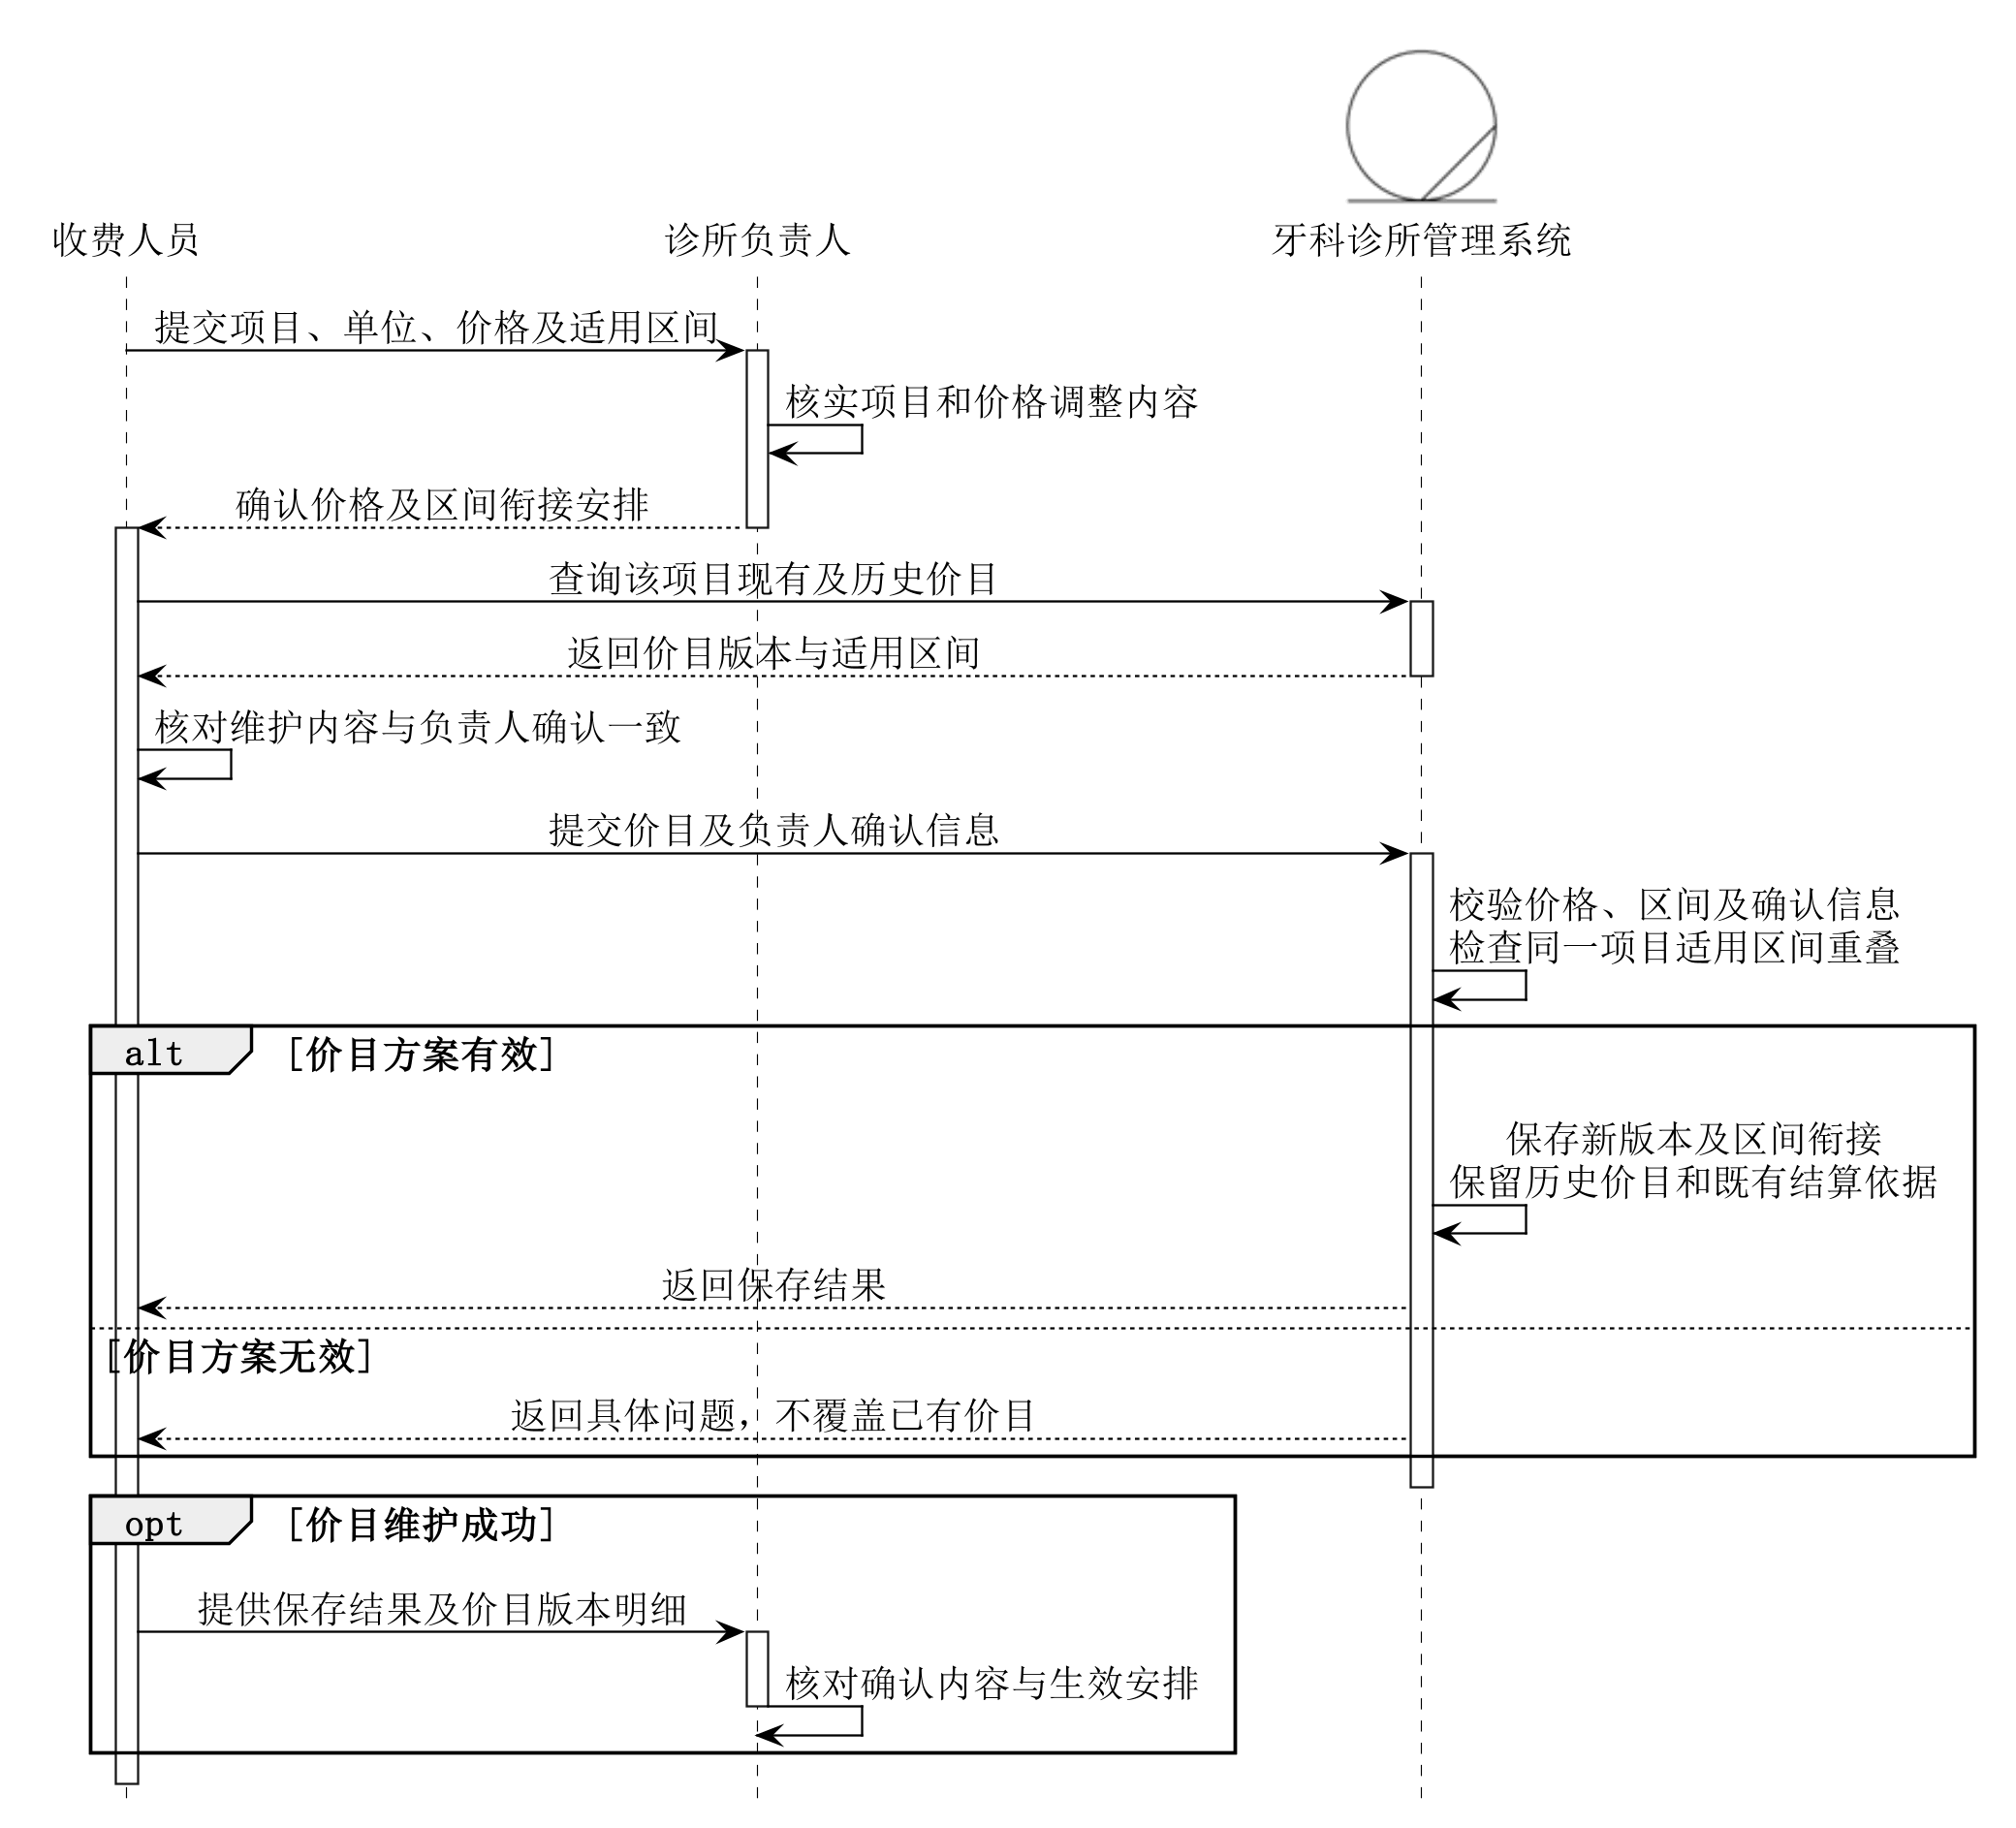
\includegraphics[width=\textwidth,height=13.4cm,keepaspectratio]{diagrams/03g-to-be-pricing.png}
\caption{改进业务序列图：价目确认与维护}
\label{fig:to-be-pricing}
\end{figure}

价目变更有明确确认责任和适用时间，项目价格能够一致使用并回查。

\clearpage
\subsubsection{材料入库、领用与盘点改进}

诊疗助理分别核对实际入库、领用或盘点数量，在系统登记办理结果。领用时先核对可用库存和实物，系统拒绝超过可用数量的领用；入库、领用及经确认的盘点调整均保留经办信息和原因。负责人查看库存及差异，确认材料补充或盘点调整。器械清洁消毒由助理按业务要求执行。

\begin{figure}[!htbp]
\centering
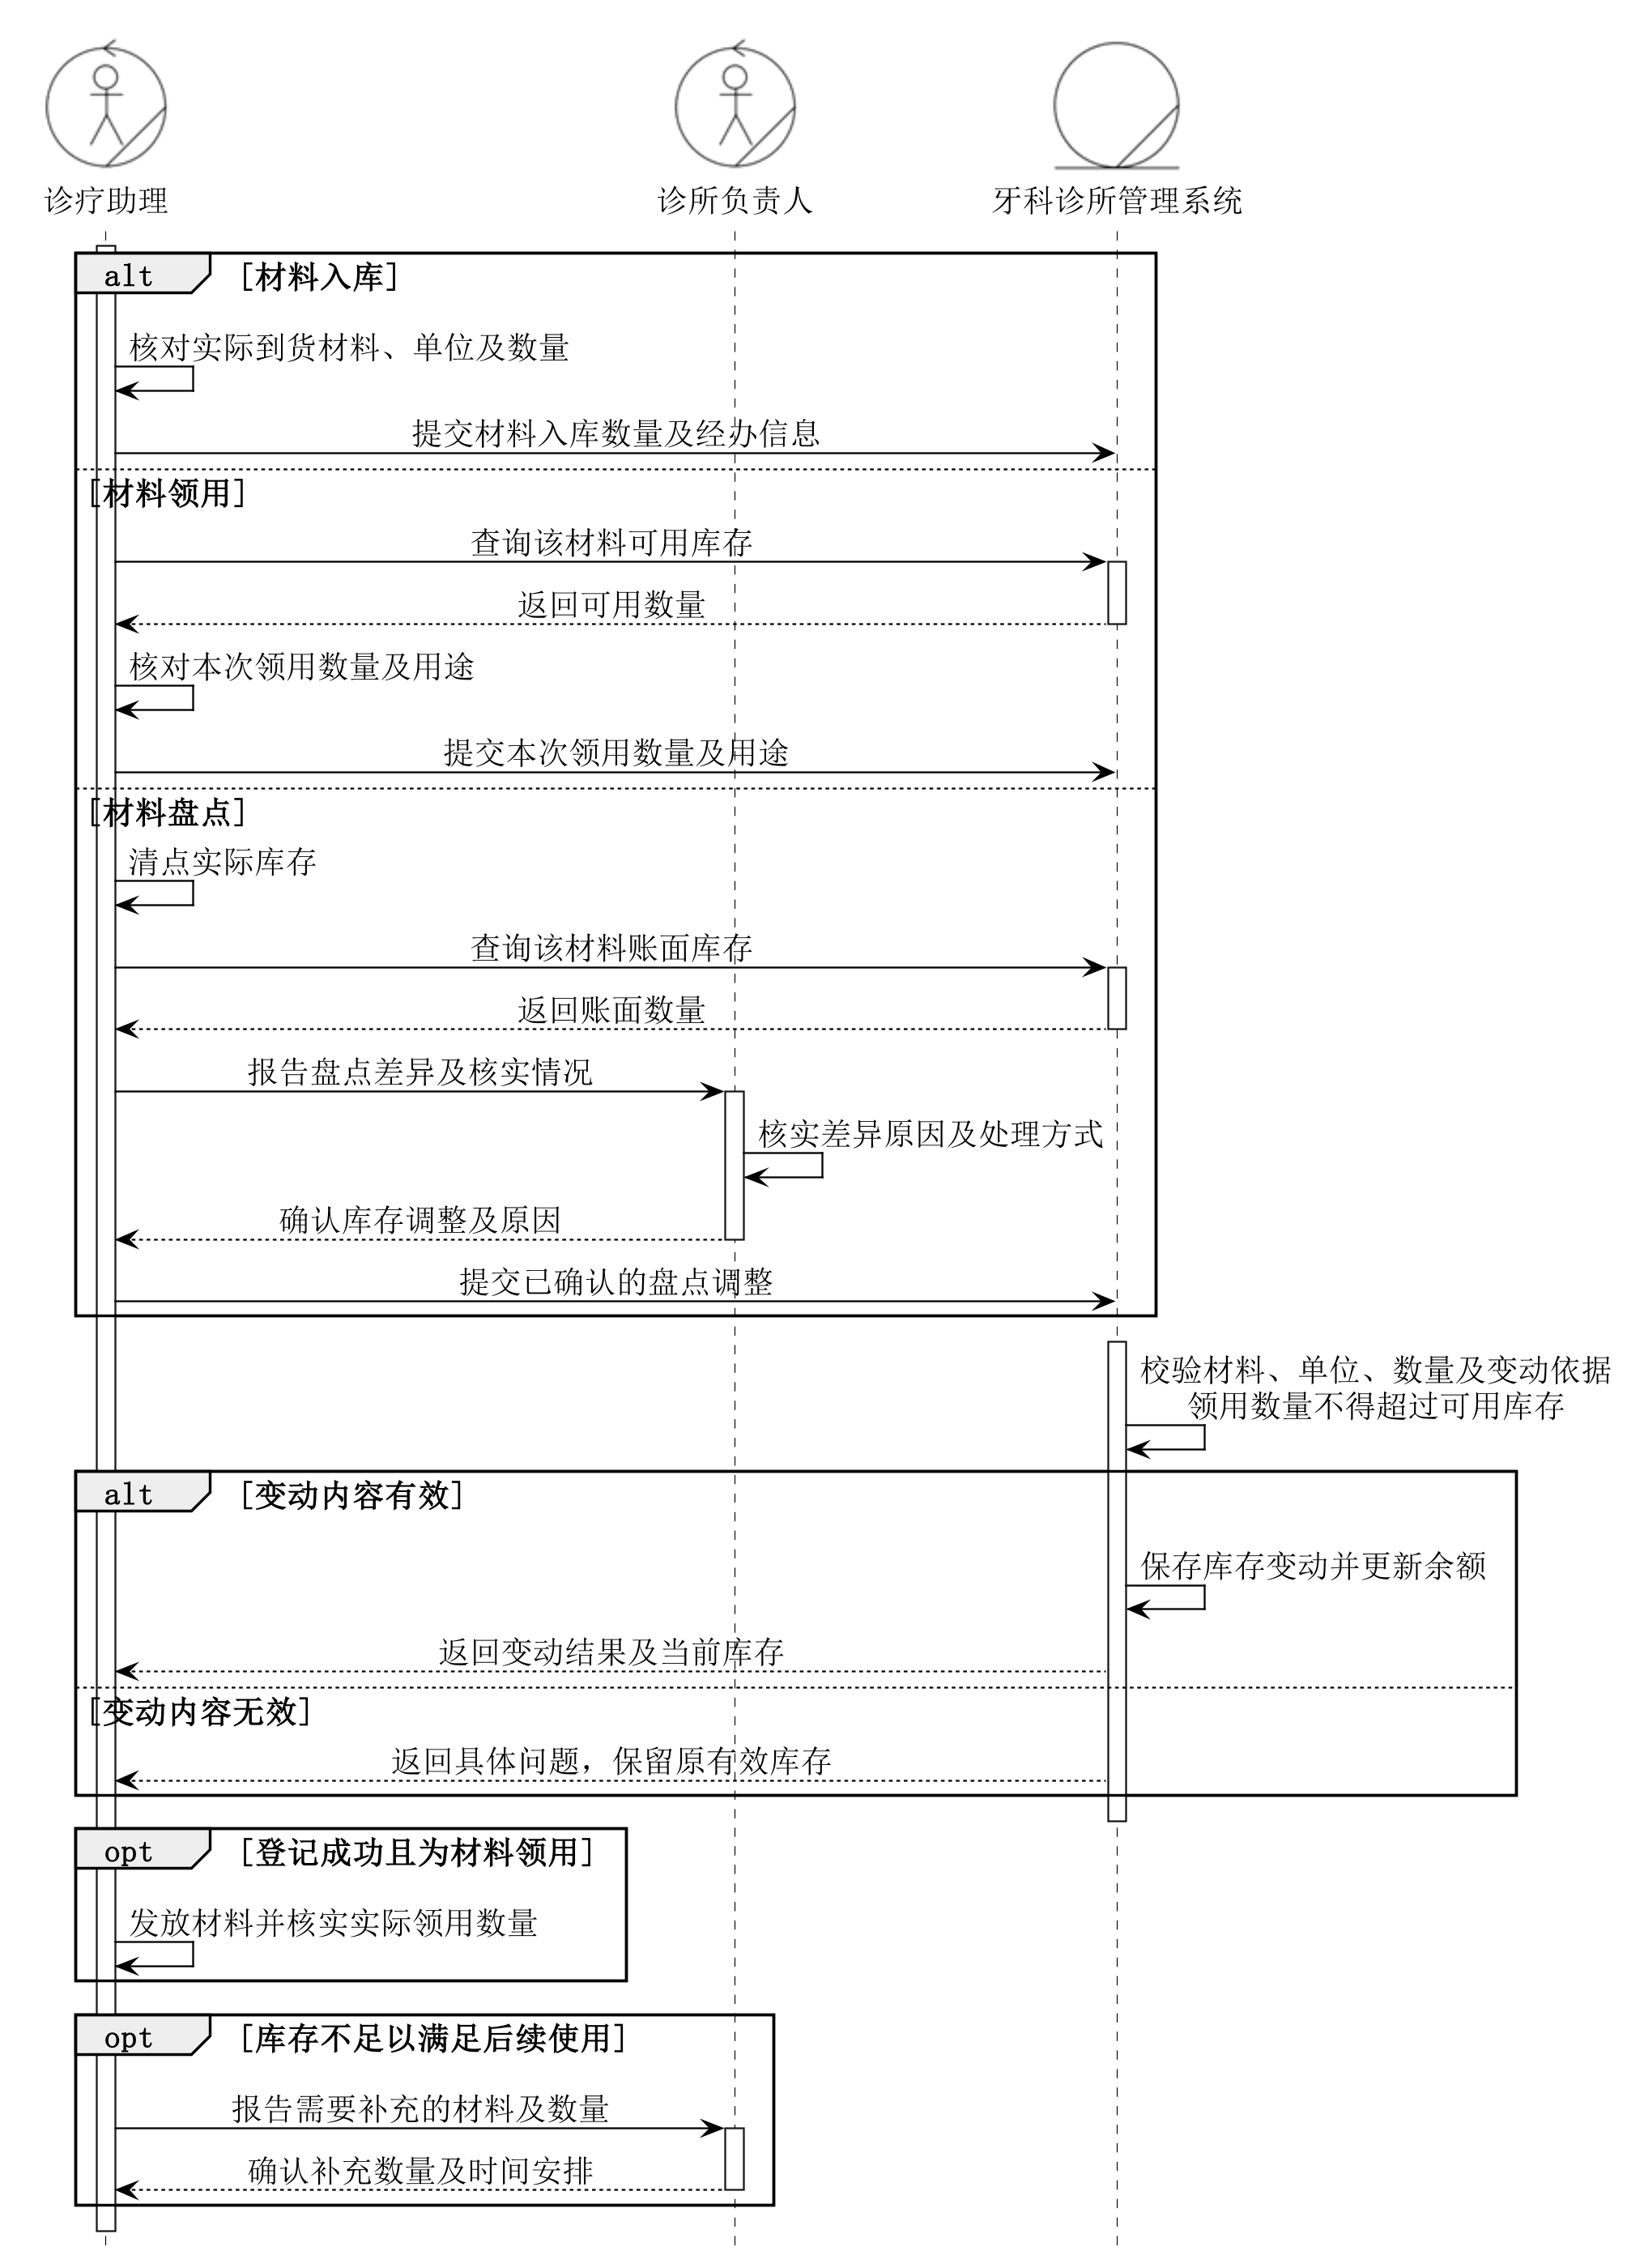
\includegraphics[width=\textwidth,height=18.0cm,keepaspectratio]{diagrams/03h-to-be-materials.png}
\caption{改进业务序列图：材料入库、领用与盘点}
\label{fig:to-be-materials}
\end{figure}

材料数量与实际收发保持对应，库存变化和差异处理可以追溯。

\clearpage
\subsubsection{日常业务与收款核对改进}

收费人员查询当日结算明细并与实际款项、凭据核对；负责人查看同一期间的就诊、项目和收款汇总。发现差异时，由相关人员核实并保存差异说明及处理结果，再确认核对情况；已经结清的收款记录保留原始依据。

\begin{figure}[!htbp]
\centering
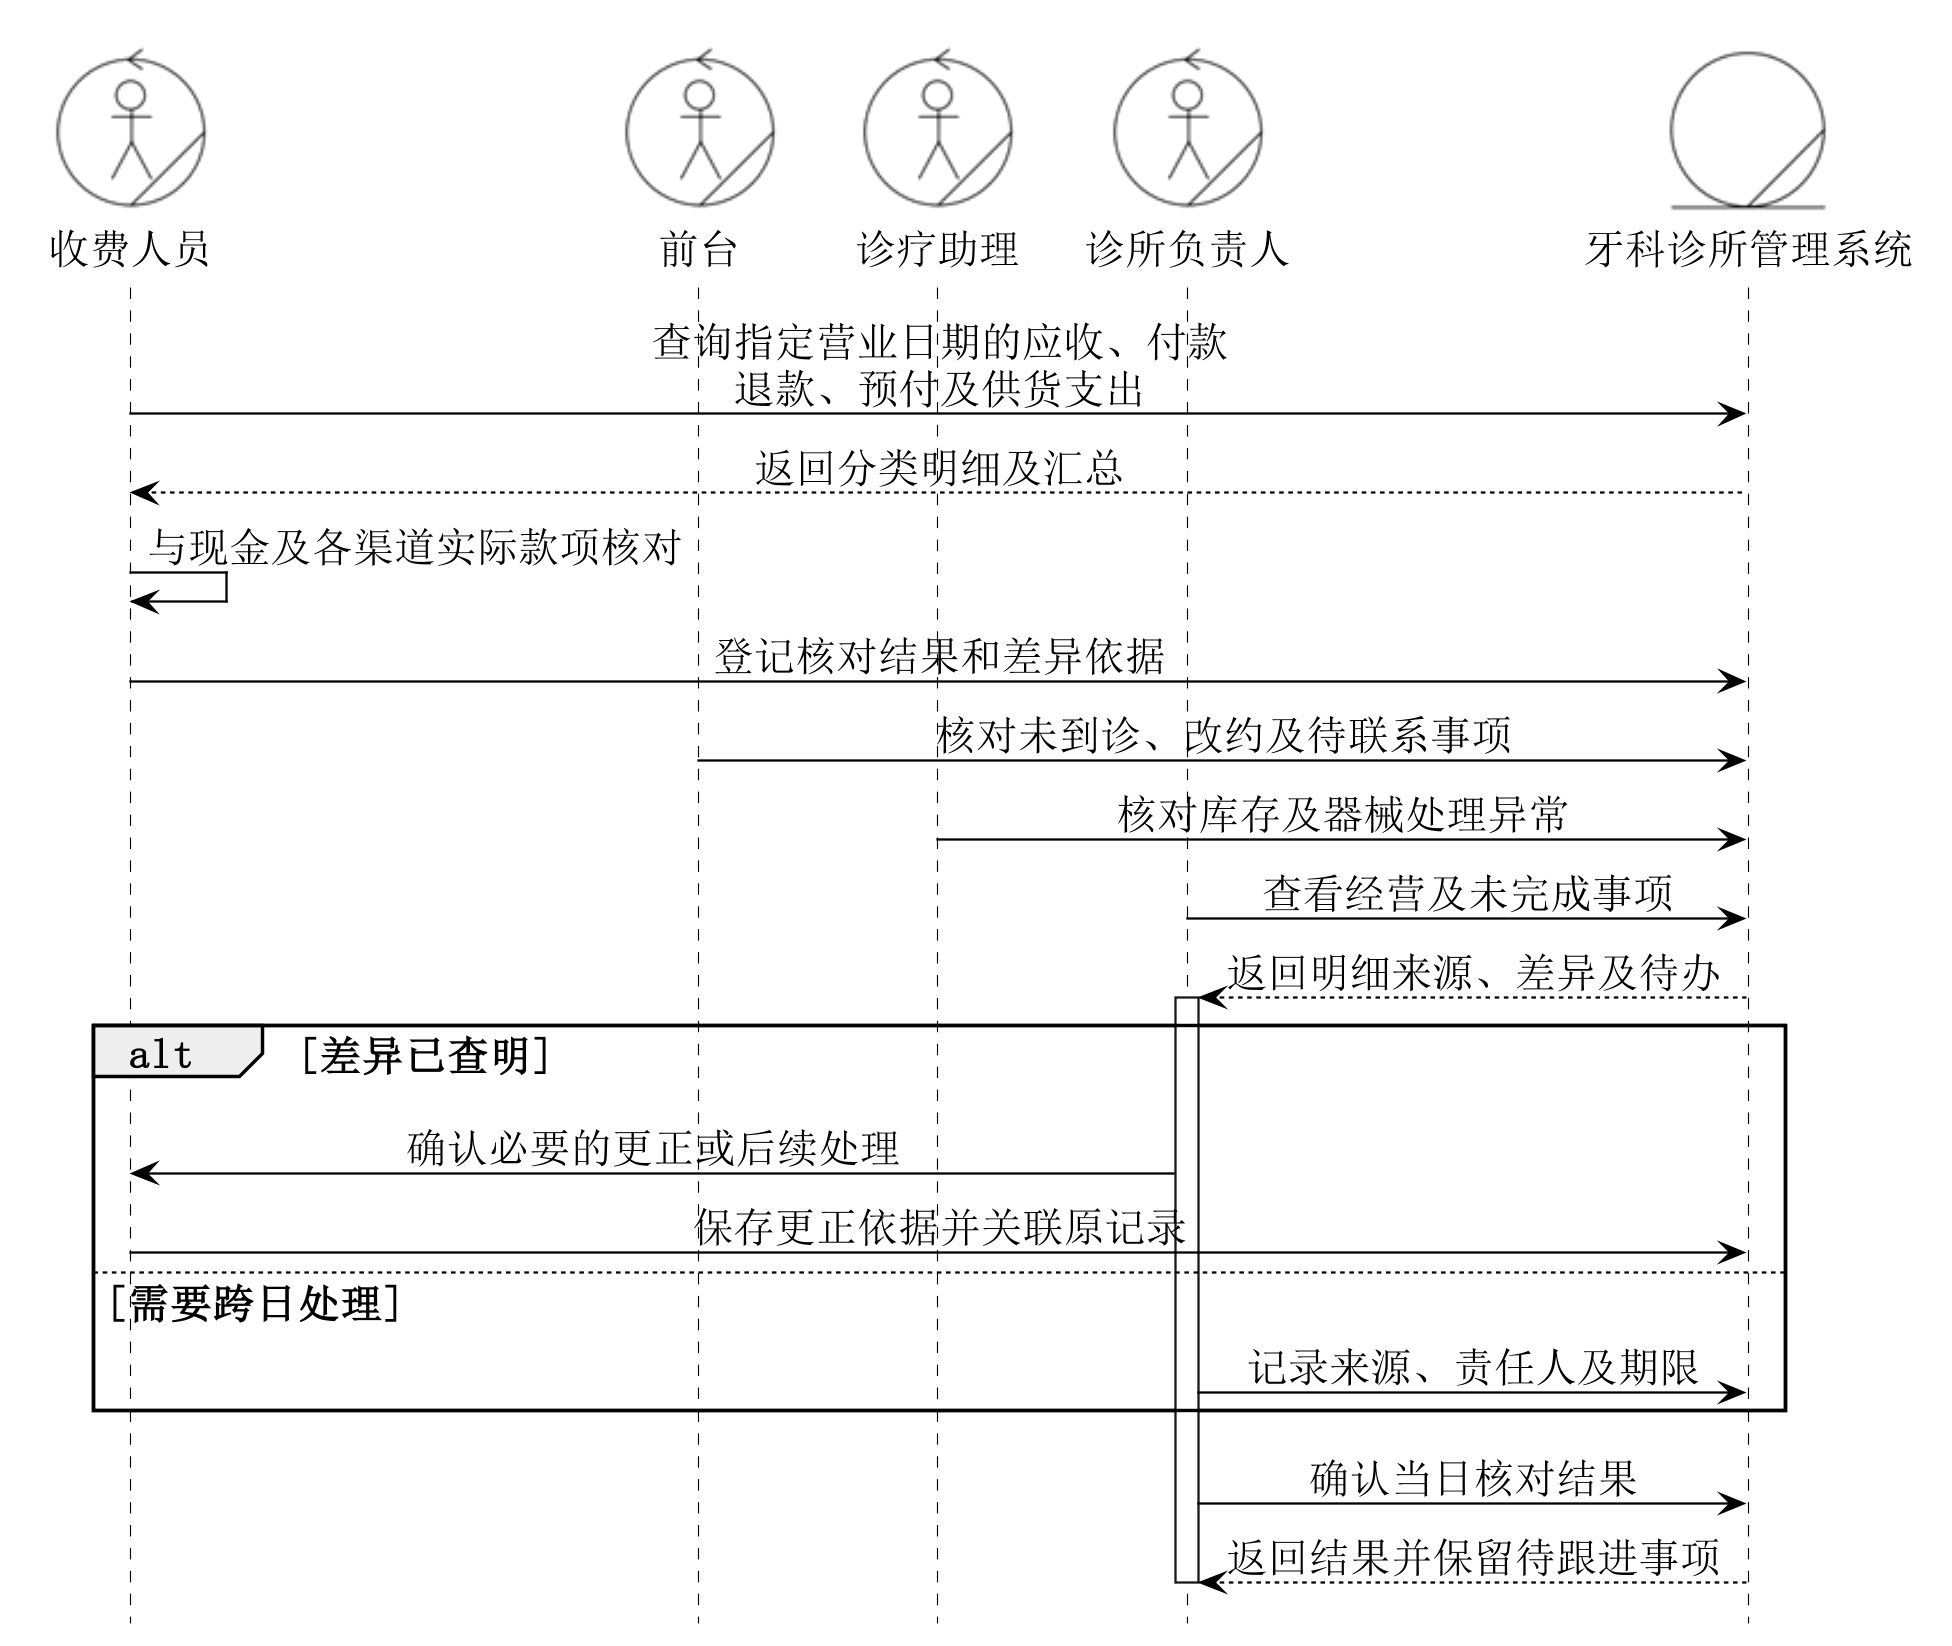
\includegraphics[width=\textwidth,height=14.0cm,keepaspectratio]{diagrams/03i-to-be-reconciliation.png}
\caption{改进业务序列图：日常业务与收款核对}
\label{fig:to-be-reconciliation}
\end{figure}

负责人获得与业务记录一致的运行情况；收款统计表示实际收入款项，不直接作为利润。

\clearpage
\section{需求}
\subsection{系统用例图}

前台、牙医、收费人员、诊疗助理和诊所负责人分别通过系统办理职责内业务。患者通过工作人员提出服务需求。以下五个岗位视图共同描述同一牙科诊所管理系统。

\begin{figure}[!htbp]
\centering
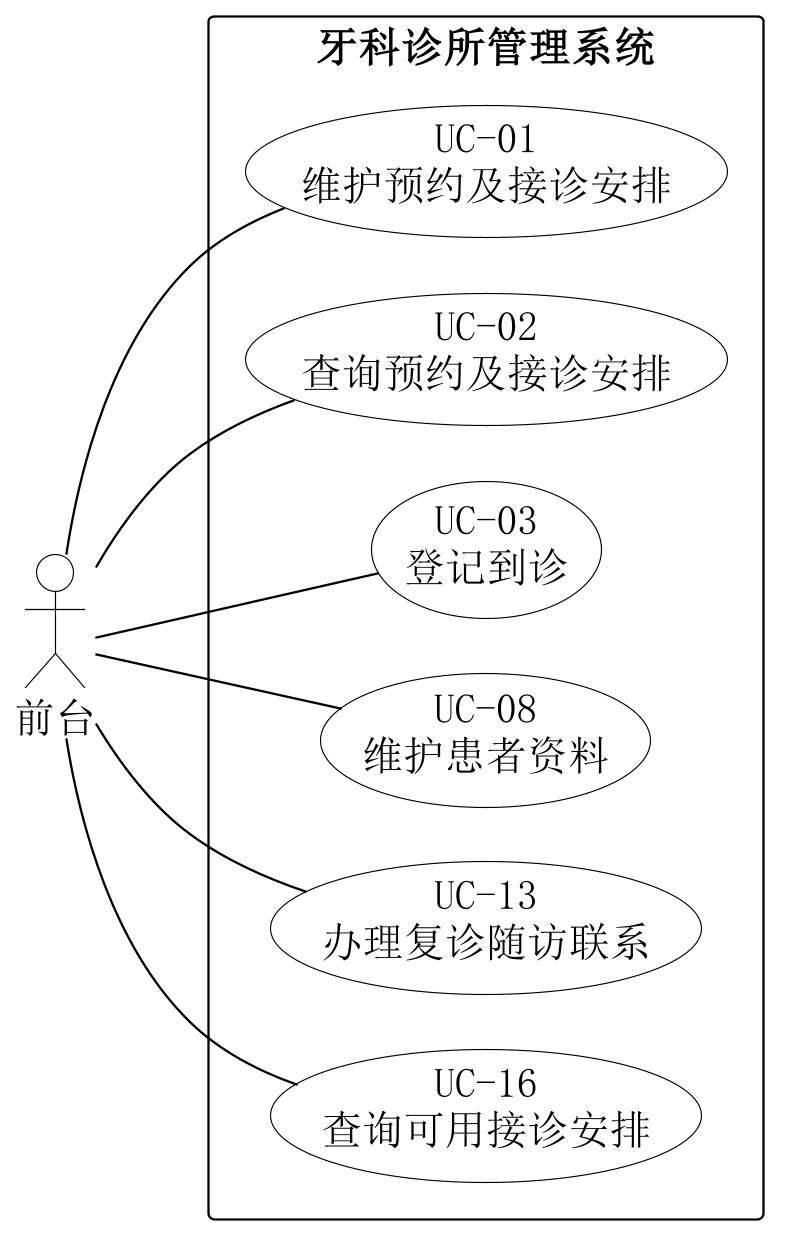
\includegraphics[width=\textwidth,height=18cm,keepaspectratio]{diagrams/07-system-use-case.png}
\caption{系统用例图：前台}
\label{fig:system-use-case}
\end{figure}
\clearpage
\begin{figure}[!htbp]
\centering
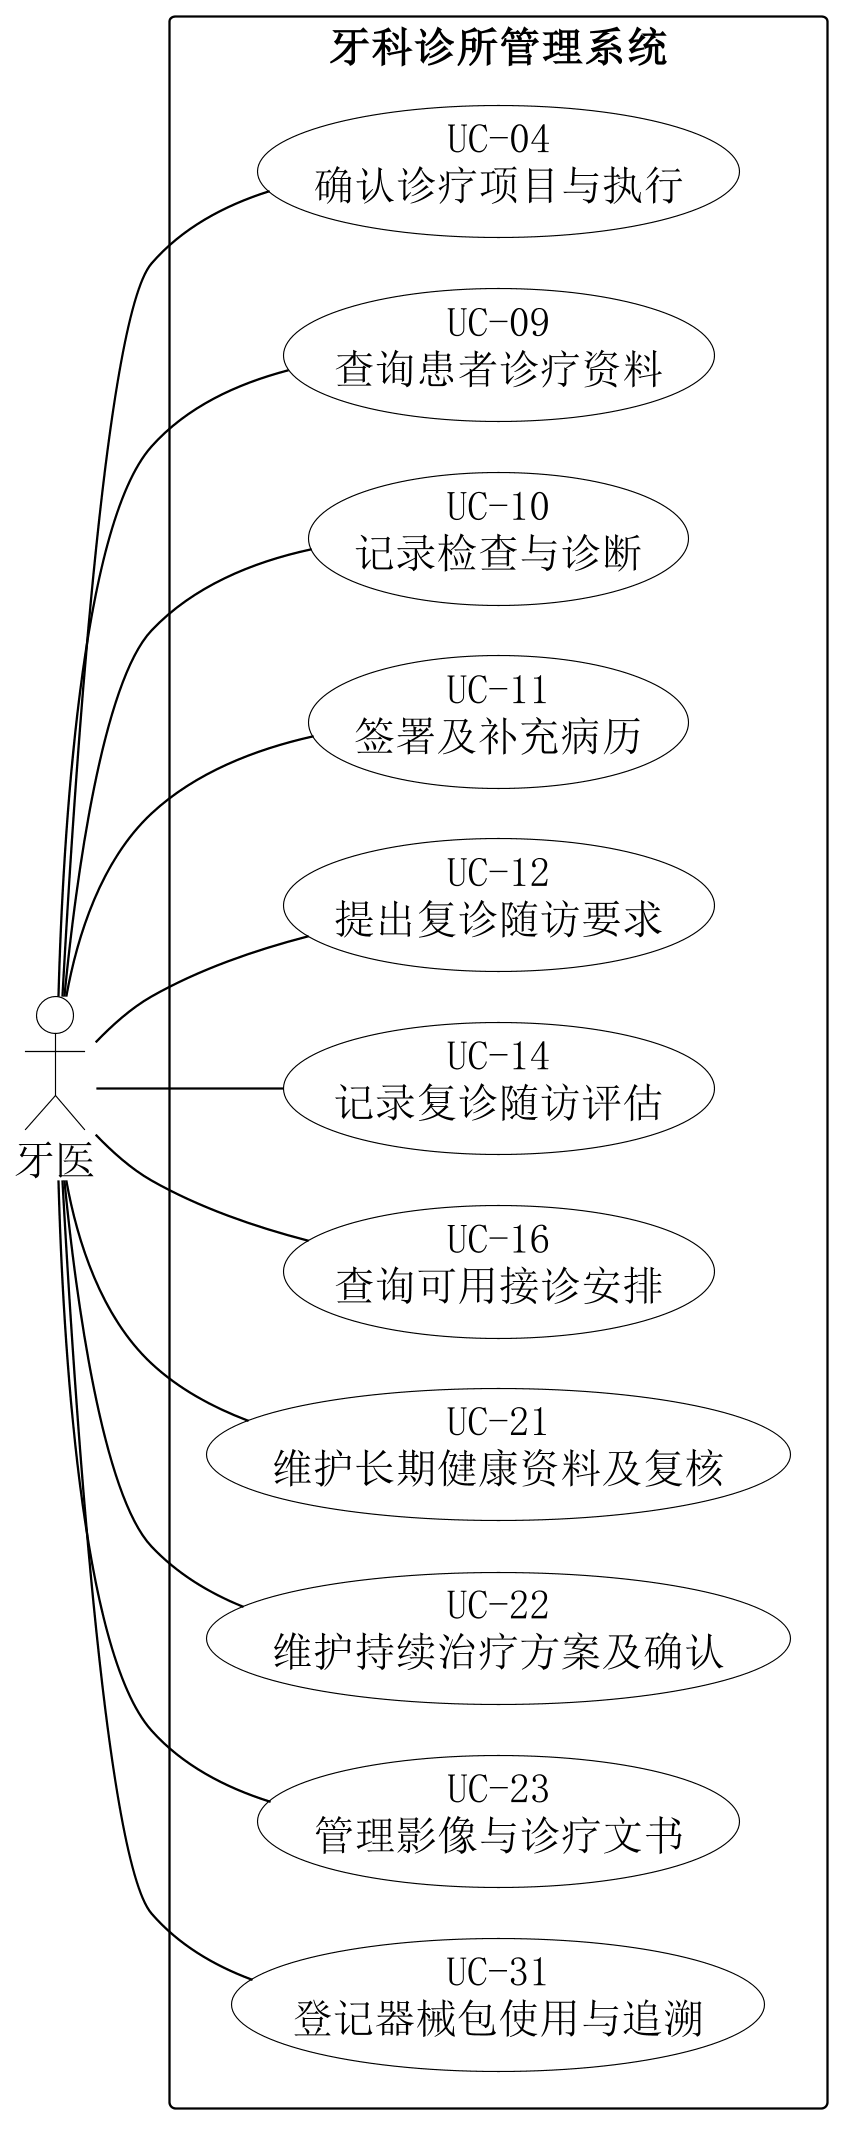
\includegraphics[width=\textwidth,height=18cm,keepaspectratio]{diagrams/07-system-dentist.png}
\caption{系统用例图：牙医}
\label{fig:system-1}
\end{figure}
\clearpage
\begin{figure}[!htbp]
\centering
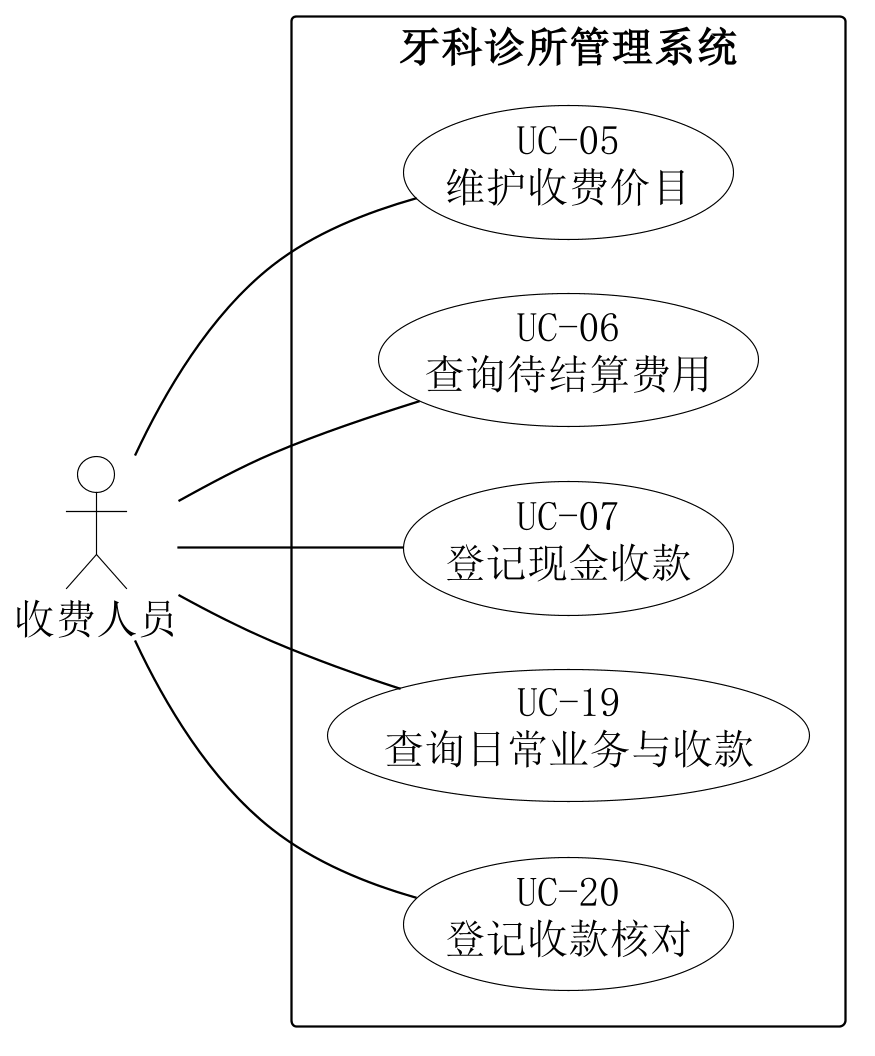
\includegraphics[width=\textwidth,height=18cm,keepaspectratio]{diagrams/07-system-cashier.png}
\caption{系统用例图：收费人员}
\label{fig:system-2}
\end{figure}
\clearpage
\begin{figure}[!htbp]
\centering
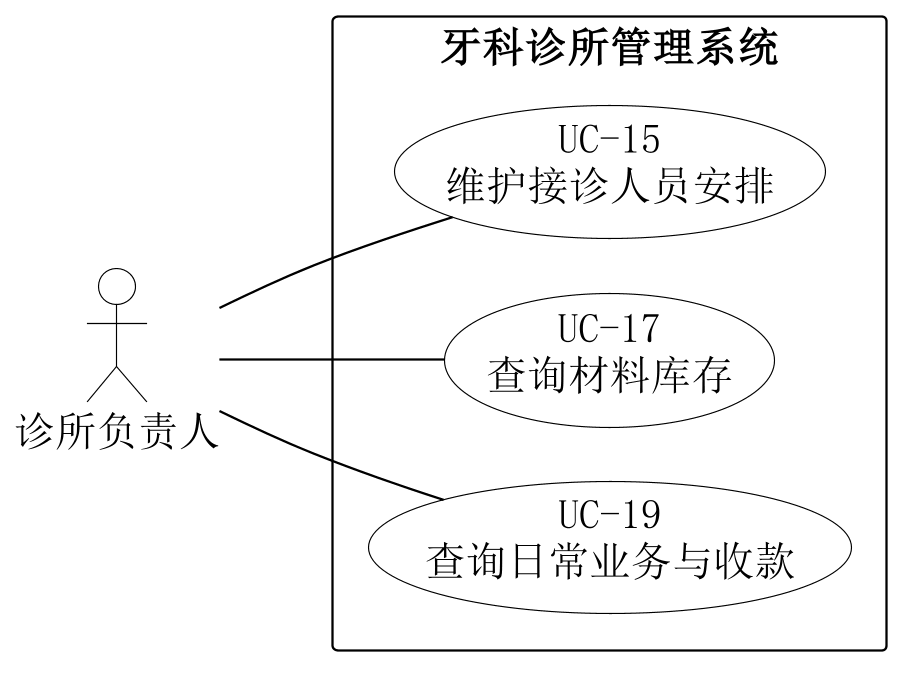
\includegraphics[width=\textwidth,height=18cm,keepaspectratio]{diagrams/07-system-manager.png}
\caption{系统用例图：诊所负责人}
\label{fig:system-3}
\end{figure}
\clearpage
\begin{figure}[!htbp]
\centering
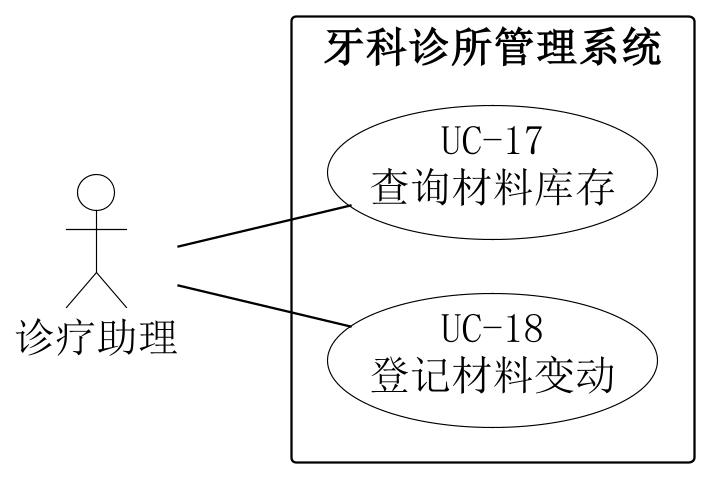
\includegraphics[width=\textwidth,height=18cm,keepaspectratio]{diagrams/07-system-assistant.png}
\caption{系统用例图：诊疗助理}
\label{fig:system-4}
\end{figure}
\clearpage
\subsubsection{系统用例范围}
{\small
\renewcommand{\arraystretch}{1.15}
\begin{longtable}{@{}>{\raggedright\arraybackslash}p{1.1cm}>{\raggedright\arraybackslash}p{3.1cm}>{\raggedright\arraybackslash}p{2.0cm}>{\raggedright\arraybackslash}p{7.9cm}@{}}
\caption{系统用例清单}\label{tab:system-use-cases}\\
\toprule
编号 & 系统用例 & 执行者 & 业务结果 \\
\midrule
\endfirsthead
\caption[]{系统用例清单（续）}\\
\toprule
编号 & 系统用例 & 执行者 & 业务结果 \\
\midrule
\endhead
\bottomrule
\endfoot
UC-01 & 维护预约及接诊安排 & 前台 & 保存经确认的预约及变更。 \\
UC-02 & 查询预约及接诊安排 & 前台 & 取得患者预约与接诊安排。 \\
UC-03 & 登记到诊 & 前台 & 关联预约并生成唯一到诊就诊。 \\
UC-04 & 确认诊疗项目 & 牙医 & 确认实际项目，形成费用依据。 \\
UC-05 & 维护收费价目 & 收费人员 & 保存负责人确认的适用价目。 \\
UC-06 & 查询待结算费用 & 收费人员 & 取得完整费用明细及核对依据。 \\
UC-07 & 登记现金收款 & 收费人员 & 保存现金收款、找零与原收据。 \\
UC-08 & 维护患者资料 & 前台 & 成功时保存患者资料及维护人、时间；修改保留原值和原因；未成功时原资料不变。 \\
UC-09 & 查询患者诊疗资料 & 牙医 & 返回选定患者本次就诊及获准的既往病历；不修改临床或收费内容。 \\
UC-10 & 记录检查诊断及方案 & 牙医 & 成功时保存本次病史、检查所见、诊断、方案及患者决定；失败时原内容保持不变。 \\
UC-11 & 签署及补充病历 & 牙医 & 签署后保留签署人、时间及原病历；补充形成独立内容与原因，不覆盖原文。 \\
UC-12 & 提出复诊随访要求 & 牙医 & 保存与来源就诊、患者关联的诊后要求、负责前台及目标日期；生成待联系事项。 \\
UC-13 & 办理复诊随访联系 & 前台 & 保存每次联系结果、经办人及时间；必要时保存下次联系日期或同患者复诊预约关联。 \\
UC-14 & 记录复诊随访评估 & 牙医 & 保存临床评估、处理意见及评估人、时间；要求进入评估完成，原联系和来源资料保留。 \\
UC-15 & 维护接诊人员安排 & 诊所负责人 & 保存经确认的接诊时段及经办人、时间；有效预约继续获得人员时段支持；失败保留原安排。 \\
UC-16 & 查询可用接诊安排 & 前台、牙医 & 返回所选日期的有效人员时段、已占用时间及可预约安排；查询不建立预约。 \\
UC-17 & 查询材料库存 & 诊疗助理、诊所负责人 & 返回材料、计量单位、账面数量及收发盘点经历；不改变库存。 \\
UC-18 & 登记材料变动 & 诊疗助理 & 成功时保留原始变动、前后数量和经办依据并更新库存；失败不改变余额或留下部分变动。 \\
UC-19 & 查询日常业务与收款 & 收费人员、诊所负责人 & 返回同期间获准的就诊、实际项目、有效现金收款及未结清明细；不改变原业务。 \\
UC-20 & 登记收款核对 & 收费人员 & 保存核对日、统计依据、实际盘点、差异及处理意见和经办时间；不改写原现金收款。 \\
\end{longtable}
}
\clearpage
\subsubsection{用例与业务流程的对应}

\begin{table}[!htbp]
\centering
\caption{业务流程与系统用例对应}
\label{tab:business-system-map}
\small
\renewcommand{\arraystretch}{1.18}
\begin{tabularx}{\textwidth}{@{}>{\raggedright\arraybackslash}p{2.2cm}>{\raggedright\arraybackslash}p{2.0cm}>{\raggedright\arraybackslash}p{4.2cm}L@{}}
\toprule
业务流程 & 业务用例 & 系统用例 & 作用 \\
\midrule
预约与到诊 & BUC-01、02 & UC-01、02、03、08、15、16 & 维护身份与确认时段，协调预约并登记到诊。 \\
检查诊断与治疗 & BUC-02、03 & UC-04、09、10、11 & 查阅与记录临床资料、患者决定，确认实际完成项目并签署病历。 \\
复诊与随访 & BUC-04 & UC-01、09、11、12、13、14 & 关联来源要求、联系及后续预约，保存临床评估。 \\
费用与收款 & BUC-05 & UC-05、06、07、19、20 & 维护适用价目、核对现金费用并保留收款与核对依据。 \\
人员与材料支持 & BUC-02、03、04 & UC-15、16、17、18 & 提供有效接诊时段及实际材料收发和盘点支持。 \\
\bottomrule
\end{tabularx}
\end{table}

查询、确认和计算是相应用例的步骤。安排确认、临床判断、患者沟通、材料清点和实际现金清点由对应岗位负责；系统记录事实并检验其关联。器械清洁消毒仍由助理按诊疗业务要求执行，不增加未建立业务依据的设备接口。
\clearpage
\subsection{系统用例规约}

以下规约分别对应UC-01至UC-20，各配一张独立系统用例图。基本路径描述成功办理，扩展路径编号对应基本路径中的步骤；前置与后置条件描述系统可检查的状态。工作人员经身份验证并取得对应权限后操作，系统在每次提交时校验权限；失去权限时拒绝操作并保留已有记录。

\begingroup
\small
\linespread{1.03}\selectfont
\setlength{\parskip}{0.15em}
\subsubsection{UC-01：维护预约及接诊安排}
\begin{figure}[htbp]
\centering
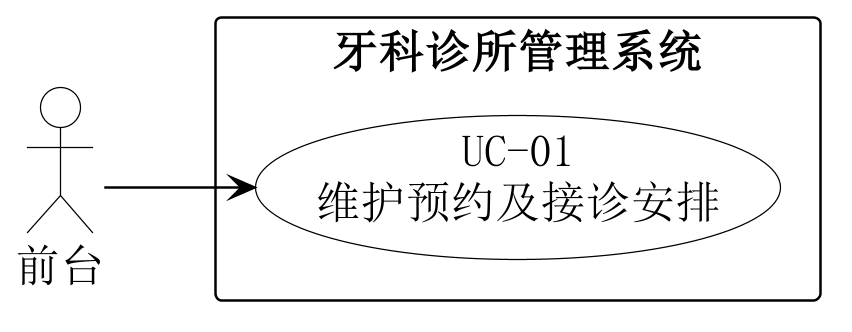
\includegraphics[width=0.82\textwidth,height=3.0cm,keepaspectratio]{diagrams/07-01-system-use-case.png}
\caption{UC-01 维护预约及接诊安排用例图}
\label{fig:uc-01}
\end{figure}
\noindent\textbf{执行者：}前台

\noindent\textbf{前置条件：}前台身份已通过验证，且具有预约维护权限。

\noindent\textbf{后置条件：}成功时保存预约编号、患者编号、时段、接诊牙医、确认依据及状态；修改和取消保留操作记录。取消关联复诊预约时，未终结的诊后要求返回待联系并保留历史依据；未成功提交时原有效内容不变。

\noindent\textbf{涉众利益：}患者希望预约安排准确；前台需要可查询的接待依据；牙医希望接诊时段不发生冲突。

\noindent\textbf{基本路径}
\begin{enumerate}
\setlength{\itemsep}{0pt}
\item 前台提交新增预约请求。
\item 前台查询并选定患者编号；系统展示姓名、电话及已发布时段的牙医确认依据。
\item 前台提交患者编号及双方约定的日期、起止时间、牙医和确认依据；排班内预约沿用该时段的牙医确认事实。
\item 系统校验必填信息、时段及接诊牙医状态，检查预约冲突。
\item 系统展示待保存的预约信息，前台确认提交。
\item 系统再次检查冲突，保存预约并返回预约编号及安排。
\end{enumerate}

\noindent\textbf{扩展路径}

\noindent\textbf{1a 修改预约：}前台选择已有预约并提交修改内容；系统展示原记录。后续按步骤4--6校验并保存，记录变更原因。

\noindent\textbf{1b 取消预约：}前台选择尚未到诊的预约并提交取消原因；系统确认记录可取消后保存取消状态并释放时段。已到诊记录不能按此路径取消。若该预约关联未终结诊后要求，系统同时将要求转为待联系，原预约及取消依据继续可查。

\noindent\textbf{2a 无患者档案或存在多个候选：}无档案时通过UC-08建档后返回步骤2；多个候选由前台核对并选定编号，不按姓名或共用电话自动合并。

\noindent\textbf{4a 信息不完整或时段冲突：}系统指出具体字段或冲突时段；前台修改后返回步骤3，或取消本次操作。

\noindent\textbf{6a 记录已被其他操作修改：}系统拒绝覆盖并展示最新记录；前台重新核对后提交。

\clearpage
\noindent\textbf{UC-01 维护预约及接诊安排（续）}
\medskip

\noindent\textbf{字段列表}

{\small
\renewcommand{\arraystretch}{1.15}
\noindent\begin{tabularx}{\textwidth}{@{}>{\raggedright\arraybackslash}p{3.5cm}>{\raggedright\arraybackslash}p{2.1cm}L@{}}
\toprule
字段 & 来源 & 约束及含义 \\
\midrule
患者编号、姓名及联系电话 & 前台选择／系统 & 患者编号必填且唯一定位已有档案；姓名、电话供核对，不能单独作为同一患者依据。 \\
预约日期、起止时间 & 前台 & 必填；结束晚于开始；新建预约开始时间不得早于当前时间。 \\
接诊牙医、安排确认信息 & 系统／前台 & 牙医须有效；保存所用时段及其牙医确认人、时间；时段调整后使用重新确认的依据。 \\
预约编号、状态、变更原因 & 系统／前台 & 编号唯一；状态为已预约、已取消或已到诊；变更须留原因。 \\
\bottomrule
\end{tabularx}
}
\medskip

\noindent\textbf{业务规则：}同一牙医的有效预约时段不得重叠；同一患者不得同时持有重叠的有效预约。已到诊记录不再作为未到诊预约修改。安排确认由牙医负责。已发布时段内的预约继承该时段的牙医确认依据；需要改变时段时先核实并通过UC-15更新安排，前台不能自行代替牙医确认。

\noindent\textbf{质量需求：}同一时段同时提交时只能保存不冲突的预约；错误提示应说明冲突时段，不泄露其他患者的姓名和电话。

\noindent\textbf{设计约束：}通过工作人员网页办理；本用例不提供患者自助预约。

\noindent\textbf{分析序列图：}基本路径见图\ref{fig:seq-01}，修改与取消预约见图\ref{fig:seq-01-ext}。

\clearpage
\subsubsection{UC-02：查询预约及接诊安排}
\begin{figure}[htbp]
\centering
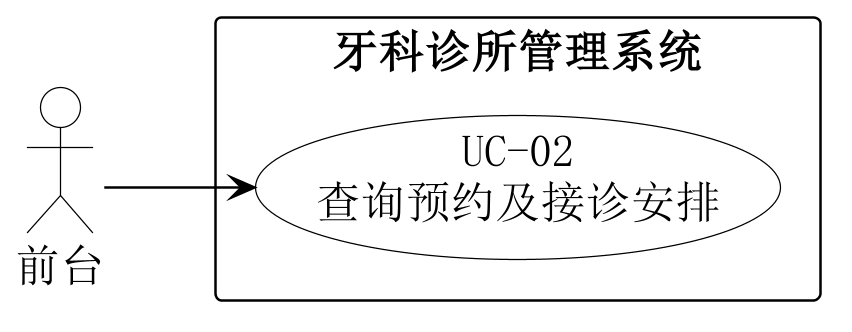
\includegraphics[width=0.82\textwidth,height=3.0cm,keepaspectratio]{diagrams/07-02-system-use-case.png}
\caption{UC-02 查询预约及接诊安排用例图}
\label{fig:uc-02}
\end{figure}
\noindent\textbf{执行者：}前台

\noindent\textbf{前置条件：}前台身份已通过验证，且具有预约查询权限。

\noindent\textbf{后置条件：}系统展示符合条件的预约列表及所选安排，或返回无匹配结果；预约状态及内容保持不变。

\noindent\textbf{涉众利益：}前台希望快速定位本次预约；患者希望身份不被混淆、个人信息不被无关人员查看。

\noindent\textbf{基本路径}
\begin{enumerate}
\setlength{\itemsep}{0pt}
\item 前台提交预约日期及患者姓名或联系电话。
\item 系统校验查询条件，并查找符合条件的预约。
\item 系统返回患者姓名、联系电话、预约时段、接诊牙医及状态。
\item 前台结合患者提供的信息选择本次预约。
\item 系统展示预约详情、候诊安排及最近更新时间。
\item 前台核对结果，结束查询或据此发起登记到诊。
\end{enumerate}

\noindent\textbf{扩展路径}

\noindent\textbf{2a 查询条件缺失：}系统指出缺少的条件；前台补充后返回步骤1。

\noindent\textbf{3a 无匹配记录：}系统返回无匹配结果；前台核对日期与患者信息后重新查询，或结束查询。

\noindent\textbf{4a 同名或存在多条预约：}前台依据联系电话、日期及预约时段核对并选择，系统不得仅按姓名代为选定。

\noindent\textbf{5a 预约已经取消或变更：}系统展示当前状态和最新安排；前台核实实际情况，不依据过期结果登记到诊。

\noindent\textbf{字段列表}

{\small
\renewcommand{\arraystretch}{1.15}
\noindent\begin{tabularx}{\textwidth}{@{}>{\raggedright\arraybackslash}p{3.5cm}>{\raggedright\arraybackslash}p{2.1cm}L@{}}
\toprule
字段 & 来源 & 约束及含义 \\
\midrule
预约日期 & 前台 & 必填；限定本次查找日期。 \\
患者姓名／联系电话 & 前台 & 至少填写一项；仅有姓名时可能返回多条记录。 \\
预约编号、时段、牙医、状态 & 系统 & 用于区分记录，展示当前有效信息。 \\
候诊安排、更新时间 & 系统 & 展示已记录的安排及最近更新时间。 \\
\bottomrule
\end{tabularx}
}
\medskip

\noindent\textbf{业务规则：}查询包括符合条件的已预约、已取消和已到诊记录，并明确区分状态。查询不产生新预约或到诊记录；身份核对由前台完成。

\noindent\textbf{质量需求：}结果为空与查询失败必须区分；多个同名结果必须可区分；查询结果仅向有权限的人员展示。

\noindent\textbf{设计约束：}查询结果可作为UC-03的选择依据；进入到诊登记时仍须重新校验预约状态。

\noindent\textbf{分析序列图：}基本路径见图\ref{fig:seq-02}。

\clearpage
\subsubsection{UC-03：登记到诊}
\begin{figure}[htbp]
\centering
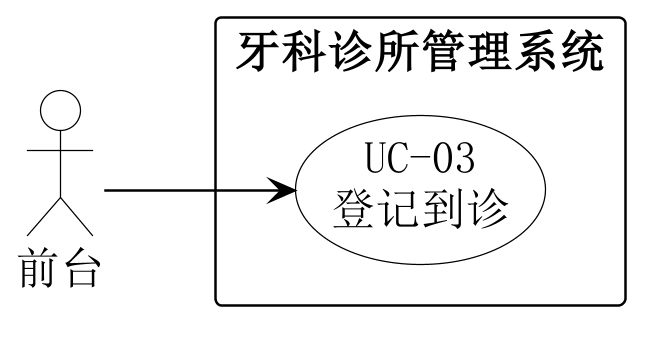
\includegraphics[width=0.82\textwidth,height=3.0cm,keepaspectratio]{diagrams/07-03-system-use-case.png}
\caption{UC-03 登记到诊用例图}
\label{fig:uc-03}
\end{figure}
\noindent\textbf{执行者：}前台

\noindent\textbf{前置条件：}前台身份已通过验证，且具有到诊登记权限。

\noindent\textbf{后置条件：}成功时生成与预约关联的唯一就诊及其病历草稿，保存到诊时间及接诊牙医，并将预约标记为已到诊；失败不产生部分结果，重复请求返回原就诊及病历。

\noindent\textbf{涉众利益：}患者希望接待正确且不重复；前台需要明确的登记结果；牙医需要一致的就诊信息。

\noindent\textbf{基本路径}
\begin{enumerate}
\setlength{\itemsep}{0pt}
\item 前台提交所选预约编号，发起到诊登记。
\item 系统展示患者身份资料、预约时段、接诊牙医及当前状态。
\item 前台核对患者与预约一致，确认登记。
\item 系统校验预约属于当日、仍为已预约状态且尚无关联到诊记录。
\item 系统生成就诊编号，建立并关联本次病历草稿，保存患者、预约及到诊时间，同时更新预约状态。
\item 系统返回登记成功、就诊编号及候诊安排，供前台告知患者。
\end{enumerate}

\noindent\textbf{扩展路径}

\noindent\textbf{3a 患者或安排不一致：}前台停止登记，重新查询或通过UC-01核实更新安排；本次不生成就诊记录。

\noindent\textbf{4a 预约非当日或已取消：}系统拒绝登记并说明原因；前台核实并调整预约后重新发起。

\noindent\textbf{4b 已经到诊或重复提交：}系统返回原就诊编号及已关联病历，不生成第二条就诊或病历。

\noindent\textbf{5a 保存失败或结果未收到：}系统不得留下预约、就诊或病历未同时完成的部分结果；前台重新查询，确认结果后再决定是否重试。

\noindent\textbf{字段列表}

{\small
\renewcommand{\arraystretch}{1.15}
\noindent\begin{tabularx}{\textwidth}{@{}>{\raggedright\arraybackslash}p{3.5cm}>{\raggedright\arraybackslash}p{2.1cm}L@{}}
\toprule
字段 & 来源 & 约束及含义 \\
\midrule
预约编号 & 前台选择 & 必填；引用系统中的预约。 \\
患者信息、接诊牙医 & 系统 & 由预约提供，展示供前台核对。 \\
就诊编号、病历编号及到诊时间 & 系统 & 就诊及本次病历各唯一；病历初始为草稿，到诊时间取成功登记时点。 \\
预约状态、候诊安排 & 系统 & 成功后为已到诊；返回对应接诊安排。 \\
\bottomrule
\end{tabularx}
}
\medskip

\noindent\textbf{业务规则：}同一预约只对应一次有效到诊登记。就诊、病历草稿与预约状态必须同时生效；重复请求返回同一组对象。到诊登记不等同于开始诊疗，不能据此填写治疗结果。

\noindent\textbf{质量需求：}并发或连续重复提交仍只形成一条登记；成功提示应包含可再次查询的就诊编号。

\noindent\textbf{设计约束：}本用例办理已有预约的当日到诊；未预约到诊须先完成预约信息登记。

\noindent\textbf{分析序列图：}基本路径见图\ref{fig:seq-03}。

\clearpage
\subsubsection{UC-04：确认诊疗项目}
\begin{figure}[htbp]
\centering
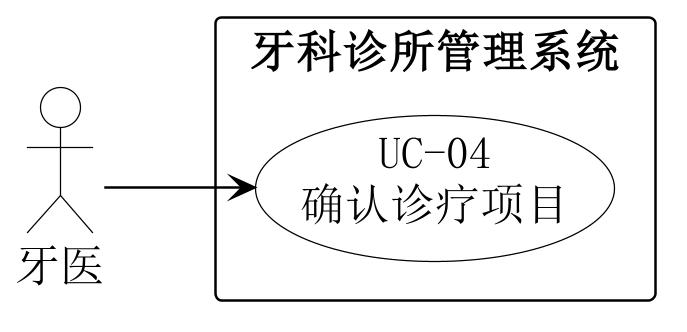
\includegraphics[width=0.82\textwidth,height=3.0cm,keepaspectratio]{diagrams/07-04-system-use-case.png}
\caption{UC-04 确认诊疗项目用例图}
\label{fig:uc-04}
\end{figure}
\noindent\textbf{执行者：}牙医

\noindent\textbf{前置条件：}牙医身份已通过验证，且具有本人接诊记录的诊疗项目确认权限。

\noindent\textbf{后置条件：}成功时保存本次已完成项目、数量、确认牙医、确认时间及记录版本，形成可计费依据；失败时保留此前有效记录。

\noindent\textbf{涉众利益：}患者希望仅对实际完成的项目收费；牙医需要准确记录诊疗事实；收费人员需要明确的计费依据。

\noindent\textbf{基本路径}
\begin{enumerate}
\setlength{\itemsep}{0pt}
\item 牙医提交本次就诊编号。
\item 系统校验就诊记录属于该牙医，展示患者及已有项目记录。
\item 牙医提交本次实际完成的诊疗项目及数量。
\item 系统校验项目有效、数量合法且本次就诊尚未结清。
\item 系统展示待确认的项目明细，牙医核对并确认提交。
\item 系统保存确认结果与版本，返回成功信息，供收费人员查询费用。
\end{enumerate}

\noindent\textbf{扩展路径}

\noindent\textbf{2a 就诊不存在或不属于该牙医：}系统拒绝操作并说明原因；牙医核对就诊编号后重新发起。

\noindent\textbf{4a 项目或数量不合法：}系统指出错误明细；牙医修正后返回步骤3。

\noindent\textbf{4b 已确认记录需要更正：}未结清时，牙医提交更正原因、原明细关联及完整项目明细；系统按既有与新增明细的计价规则保存新版本，重算方案有效数量并使旧费用核对结果失效。已结清时拒绝覆盖。

\noindent\textbf{6a 记录版本变化或已经结清：}系统拒绝保存过期内容，保留当前有效记录；牙医重新核对。

\clearpage
\noindent\textbf{UC-04 确认诊疗项目（续）}
\medskip

\noindent\textbf{字段列表}

{\small
\renewcommand{\arraystretch}{1.15}
\noindent\begin{tabularx}{\textwidth}{@{}>{\raggedright\arraybackslash}p{3.5cm}>{\raggedright\arraybackslash}p{2.1cm}L@{}}
\toprule
字段 & 来源 & 约束及含义 \\
\midrule
就诊编号 & 牙医选择 & 必填；须属于本人接诊范围。 \\
项目编号、牙位、数量 & 牙医 & 至少一项；数量为正整数；同项目、同牙位且依据一致的重复明细合并，不同牙位分别保留。 \\
实际完成时间、方案依据 & 牙医 & 完成时间不早于本次到诊且不晚于提交时间；方案内填写本次方案项目编号，方案外填写原因及患者确认事实。 \\
原明细编号、计价时点 & 牙医选择／系统 & 更正时原明细须属本次就诊的当前版本；未更换收费项目时继承原计价时点和价目，新增或更换项目时取本次确认时点。 \\
确认人、确认时间、版本 & 系统 & 记录实际操作者及确认时间；更正形成新版本。 \\
更正原因 & 牙医 & 修改已确认项目时必填，保留原版本。 \\
\bottomrule
\end{tabularx}
}
\medskip

\noindent\textbf{业务规则：}仅确认实际完成的项目；同一项目、同一牙位且方案、计价与完成日期依据一致的重复明细合并数量，不同牙位分别保留；依据不一致时须核实归属。更正同一收费项目的既有明细时，牙位或数量变更仍继承原计价时点及原价目；新增或更换收费项目按本次确认时点匹配，缺价既有行仍按原计价时点补齐。方案内项目须属于本次就诊、患者已同意；按拟生效完整明细集合校验预计数量，更正成功后替换当前版本重算，历史版本不重复累计。方案外项目须保存原因及患者确认事实。已结清项目不得直接覆盖，结算后的更正另行处理。

\noindent\textbf{质量需求：}保留确认及更正记录；项目变更后，收费人员不能使用旧项目版本完成收款登记。

\noindent\textbf{设计约束：}由牙医使用网页提交确认；系统记录确认事实，不替代牙医判断实际治疗内容。

\noindent\textbf{分析序列图：}基本路径见图\ref{fig:seq-04}，更正诊疗项目见图\ref{fig:seq-04-ext}。

\clearpage
\subsubsection{UC-05：维护收费价目}
\begin{figure}[htbp]
\centering
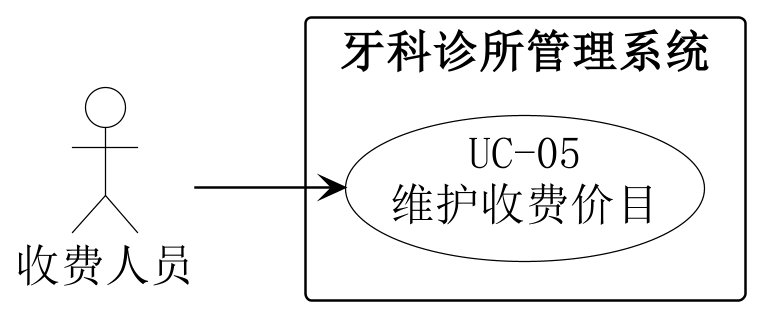
\includegraphics[width=0.82\textwidth,height=3.0cm,keepaspectratio]{diagrams/07-05-system-use-case.png}
\caption{UC-05 维护收费价目用例图}
\label{fig:uc-05}
\end{figure}
\noindent\textbf{执行者：}收费人员

\noindent\textbf{前置条件：}收费人员身份已通过验证，且具有收费价目维护权限。

\noindent\textbf{后置条件：}成功时保存项目价目版本、计价单位、金额、适用起止时间和负责人确认信息；历史价目及已结算金额保持可追溯。

\noindent\textbf{涉众利益：}患者希望收费有依据；负责人希望确认的价目被正确执行；收费人员希望计费时能确定唯一适用价格。

\noindent\textbf{基本路径}
\begin{enumerate}
\setlength{\itemsep}{0pt}
\item 收费人员提交新增或调整收费项目价目的请求。
\item 系统展示项目现有价目及适用时间。
\item 收费人员提交经负责人确认的新价目及确认信息。
\item 系统校验项目、计价单位、单价、适用时间及版本重叠情况。
\item 系统展示待保存价目，收费人员核对并确认提交。
\item 系统保存新版本和操作记录，返回价目编号及适用时间。
\end{enumerate}

\noindent\textbf{扩展路径}

\noindent\textbf{3a 停用收费项目：}收费人员提交负责人确认的停止适用时间；系统结束对应价目的适用区间，保留历史记录。

\noindent\textbf{4a 金额、时间或确认信息不合法：}系统指出错误；收费人员更正后返回步骤3。

\noindent\textbf{4b 新版本与原版本重叠：}系统提示冲突；收费人员明确原版本结束时间后重新提交，系统一并校验并保存衔接后的区间。

\noindent\textbf{6a 当前价目已被其他操作调整：}系统拒绝覆盖，要求核对最新版本后重新提交。

\noindent\textbf{字段列表}

{\small
\renewcommand{\arraystretch}{1.15}
\noindent\begin{tabularx}{\textwidth}{@{}>{\raggedright\arraybackslash}p{3.5cm}>{\raggedright\arraybackslash}p{2.1cm}L@{}}
\toprule
字段 & 来源 & 约束及含义 \\
\midrule
项目编号、名称、计价单位 & 收费人员 & 编号唯一；单位须明确，例如次或颗。 \\
单价 & 收费人员 & 人民币元，精确到分，金额不得为负。 \\
适用起止时间 & 收费人员 & 起点必填；终点可空表示持续有效；结束晚于开始。 \\
负责人确认信息、调整原因 & 收费人员 & 记录确认人及时间；调整时填写原因。 \\
\bottomrule
\end{tabularx}
}
\medskip

\noindent\textbf{业务规则：}同一项目在同一时点至多有一个有效价目；适用区间包含开始时点、不包含结束时点。新增或更换收费项目的明细按其首次确认时点匹配价目并保存计价时点；更正同一收费项目的既有明细沿用原计价时点及已保留价目。后续调价不改变这些已有明细的单价；原缺价行补齐时仍按原计价时点匹配。

\noindent\textbf{质量需求：}并发调整不能形成重叠价目；历史版本可查询，错误提示须定位冲突的适用区间。

\noindent\textbf{设计约束：}负责人线下确认后由收费人员维护；系统校验确认信息是否完整，不承担线上审批。

\noindent\textbf{分析序列图：}基本路径见图\ref{fig:seq-05}，停止适用与价目区间衔接见图\ref{fig:seq-05-ext}。

\clearpage
\subsubsection{UC-06：查询待结算费用}
\begin{figure}[htbp]
\centering
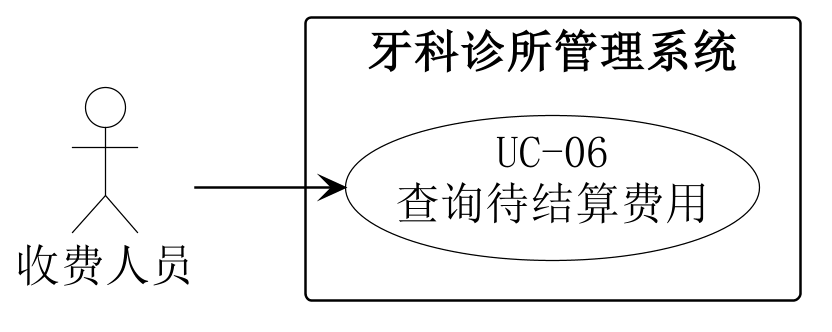
\includegraphics[width=0.82\textwidth,height=3.0cm,keepaspectratio]{diagrams/07-06-system-use-case.png}
\caption{UC-06 查询待结算费用用例图}
\label{fig:uc-06}
\end{figure}
\noindent\textbf{执行者：}收费人员

\noindent\textbf{前置条件：}收费人员身份已通过验证，且具有费用查询权限。

\noindent\textbf{后置条件：}成功时返回对应就诊的收费明细、应收金额及其项目版本、价目依据；查询不新增收款，也不改变结清状态。

\noindent\textbf{涉众利益：}患者希望逐项核对费用；收费人员需要完整且一致的应收金额；牙医希望项目确认结果被准确用于计费。

\noindent\textbf{基本路径}
\begin{enumerate}
\setlength{\itemsep}{0pt}
\item 收费人员提交患者信息或就诊编号。
\item 系统展示匹配的就诊记录及结算状态。
\item 收费人员核实患者及本次就诊，选择待结算记录。
\item 系统检查项目已确认、数量合法且具备对应适用价目，逐项计算金额并汇总。
\item 系统返回项目名称、数量、单位、单价、明细金额、应收总额及费用核对版本。
\item 收费人员据此与患者核对费用，结束查询或发起现金收款登记。
\end{enumerate}

\noindent\textbf{扩展路径}

\noindent\textbf{2a 无记录或存在多个同名患者：}系统展示无结果或候选记录；收费人员核对身份及就诊日期后重新选择。

\noindent\textbf{4a 项目尚未确认或价格缺失：}系统提示具体问题，不把缺失项按零元计算；相关岗位处理完成后重新查询。

\noindent\textbf{4b 本次就诊已结清：}系统展示结算状态和既有收款结果，不再提供待收款操作。

\noindent\textbf{5a 核对期间项目被更正：}原核对结果不得用于登记收款；收费人员重新查询最新版本并与患者核对。

\noindent\textbf{字段列表}

{\small
\renewcommand{\arraystretch}{1.15}
\noindent\begin{tabularx}{\textwidth}{@{}>{\raggedright\arraybackslash}p{3.5cm}>{\raggedright\arraybackslash}p{2.1cm}L@{}}
\toprule
字段 & 来源 & 约束及含义 \\
\midrule
患者信息／就诊编号 & 收费人员 & 至少提供可定位记录的条件；最终选定唯一就诊。 \\
项目、数量、单位及单价 & 系统 & 来自已确认项目及适用价目依据。 \\
明细金额、应收总额 & 系统 & 人民币元，精确到分；合计须与明细一致。 \\
费用核对版本、结算状态 & 系统 & 用于后续收款时核验内容是否变化。 \\
\bottomrule
\end{tabularx}
}
\medskip

\noindent\textbf{业务规则：}各项金额为确认数量乘以对应单价，应收金额为各项之和。使用十进制金额精确到分；缺失价目不能视为免费。已有价目为零时按其有效价目处理。

\noindent\textbf{质量需求：}同一项目版本和价格依据应得到一致金额；查询失败不得显示为零费用或已结清。

\noindent\textbf{设计约束：}本用例提供费用核对依据；实际现金清点由收费人员完成。

\noindent\textbf{分析序列图：}基本路径见图\ref{fig:seq-06}。

\clearpage
\subsubsection{UC-07：登记现金收款}
\begin{figure}[htbp]
\centering
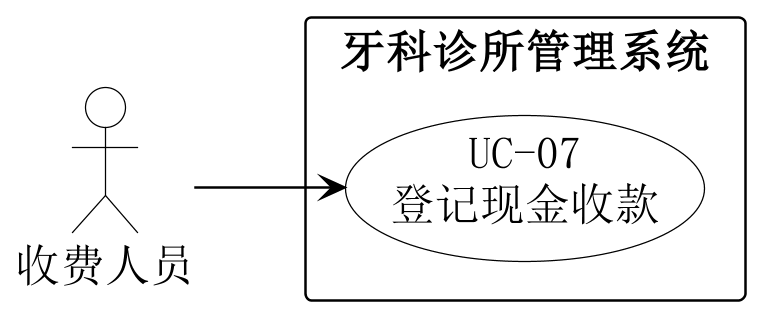
\includegraphics[width=0.82\textwidth,height=3.0cm,keepaspectratio]{diagrams/07-07-system-use-case.png}
\caption{UC-07 登记现金收款用例图}
\label{fig:uc-07}
\end{figure}
\noindent\textbf{执行者：}收费人员

\noindent\textbf{前置条件：}收费人员身份已通过验证，且具有现金收款登记权限。

\noindent\textbf{后置条件：}成功时保存唯一收款编号、就诊编号、费用依据、实际交付金额、找零、净收金额及操作人，并将本次就诊标记为结清；失败时不产生部分收款记录。

\noindent\textbf{涉众利益：}患者希望金额和找零正确且不被重复收费；收费人员需要可靠凭据；负责人希望收入记录可核对。

\noindent\textbf{基本路径}
\begin{enumerate}
\setlength{\itemsep}{0pt}
\item 收费人员提交本次就诊编号及已核对的费用版本。
\item 系统重新检查未结清状态和费用依据，展示应收金额。
\item 收费人员清点患者交付的现金后，提交实际收到金额并确认登记。
\item 系统校验金额足以结清，计算找零，并再次检查费用版本及结算状态。
\item 系统同时保存收款记录和结清状态，记录操作人及时间。
\item 系统返回收款编号、金额、找零及收据，供收费人员交付患者。
\end{enumerate}

\noindent\textbf{扩展路径}

\noindent\textbf{2a 项目或价目依据与核对结果不一致：}系统停止登记；收费人员通过UC-06重新核对费用，不能直接沿用原应收金额。

\noindent\textbf{4a 金额不足或格式错误：}系统拒绝结清；收费人员核实后修改金额或取消。该路径不登记部分收款，也不自动形成欠费记录。

\noindent\textbf{4b 已结清或重复提交：}系统返回已有收款结果；同一就诊不再次生成收款，收费人员依据结果核对实际现金。

\noindent\textbf{5a 保存失败或结果未收到：}系统保证收款与结清同时生效；收费人员先查询状态，再决定是否重试，不能仅凭未收到提示重复收费。

\noindent\textbf{6a 收据未能输出：}既有收款仍有效；收费人员重新取得原编号收据，不重新登记收款。

\clearpage
\noindent\textbf{UC-07 登记现金收款（续）}
\medskip

\noindent\textbf{字段列表}

{\small
\renewcommand{\arraystretch}{1.15}
\noindent\begin{tabularx}{\textwidth}{@{}>{\raggedright\arraybackslash}p{3.5cm}>{\raggedright\arraybackslash}p{2.1cm}L@{}}
\toprule
字段 & 来源 & 约束及含义 \\
\midrule
就诊编号、费用核对版本 & 收费人员选择 & 必填；与本次已核对费用一致。 \\
实际收到金额 & 收费人员 & 人民币元、精确到分；本场景须不低于应收金额。 \\
应收、找零、净收金额 & 系统 & 找零＝实际收到－应收；净收＝应收。 \\
收款编号、时间、操作人 & 系统 & 编号唯一，时间及操作人随成功登记保存。 \\
\bottomrule
\end{tabularx}
}
\medskip

\noindent\textbf{业务规则：}同一就诊只允许一次有效的足额现金结算；重复提交返回原结果。收款记录与结清状态必须同时生效；已结清记录不得通过重提覆盖。

\noindent\textbf{质量需求：}并发提交只能形成一次有效收款；金额计算精确到分；收据内容必须与已保存的收款记录一致。

\noindent\textbf{设计约束：}仅登记现金足额结算，不调用第三方支付接口；退款及部分收款不在本用例范围内。



\noindent\textbf{分析序列图：}基本路径见图\ref{fig:seq-07}，重复提交与结果恢复见图\ref{fig:seq-07-ext}。

\clearpage
\clearpage
\subsubsection{UC-08：维护患者资料}
\begin{figure}[!htbp]
\centering
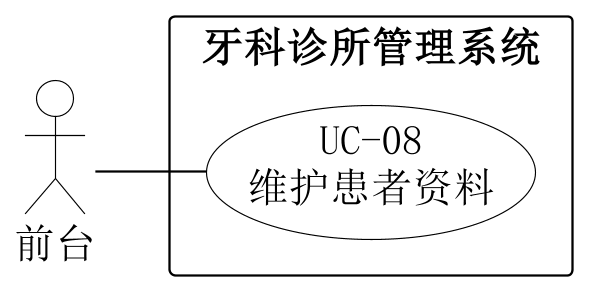
\includegraphics[width=0.90\textwidth,height=2.8cm,keepaspectratio]{diagrams/07-08-system-use-case.png}
\caption{UC-08 维护患者资料用例图}
\label{fig:uc-08}
\end{figure}
\noindent\textbf{执行者：}前台

\noindent\textbf{前置条件：}前台身份有效，具有患者资料维护权限。

\noindent\textbf{后置条件：}成功时保存患者资料及维护人、时间；修改保留原值和原因；未成功时原资料不变。

\noindent\textbf{涉众利益：}患者希望身份和联系方式正确；牙医需要连续诊疗依据；前台需要避免同名误选。

\noindent\textbf{基本路径}
\begin{enumerate}\setlength{\itemsep}{0pt}
\item 前台提交新增或修改患者资料请求。
\item 系统反馈已有资料及相似患者，提示需要核对的信息。
\item 前台提交核对后的姓名、联系方式及资料；修改时提交原因。
\item 系统校验资料完整性，核对选定患者和相似资料。
\item 前台确认所维护的患者及资料。
\item 系统再次核对原资料，保存结果并反馈患者编号。
\end{enumerate}

\noindent\textbf{扩展路径}

\noindent\textbf{2a 存在同名或相同电话：}系统反馈候选患者；前台核对身份后选用已有患者，或确认确为不同患者后继续新增，不自动合并。

\noindent\textbf{4a 必填资料缺失：}系统指出缺项，前台修正后返回步骤3。

\noindent\textbf{6a 资料已被修改：}系统拒绝覆盖，反馈最新资料，前台重新核对。

\begin{table}[!htbp]
\centering
\caption{UC-08 输入与输出字段}
\label{tab:fields-08}
\small
\renewcommand{\arraystretch}{1.18}
\begin{tabularx}{\textwidth}{@{}>{\raggedright\arraybackslash}p{3.3cm}>{\raggedright\arraybackslash}p{2.0cm}L@{}}
\toprule
字段 & 来源 & 约束及含义 \\
\midrule
患者姓名、联系电话 & 前台 & 必填；联系电话按诊所采用的号码格式校验。 \\
出生日期、其他身份说明 & 前台 & 有明确依据时填写；未知内容不编造。 \\
患者编号、维护人及时间 & 系统 & 编号唯一，修改不得改变患者的业务归属。 \\
修改原因、原资料 & 前台／系统 & 修改时保存；原值可回查。 \\
\bottomrule
\end{tabularx}
\end{table}

\noindent\textbf{业务规则：}同名或共用电话不足以判定为同一患者。预约、病历及收款依患者编号关联；本用例不删除、合并或迁移已有诊疗。

\noindent\textbf{质量需求：}一次失败提交不改变任何原资料；相似提示只提供当前岗位可核对的身份信息。

\noindent\textbf{设计约束：}由前台使用工作人员网页办理。

\noindent\textbf{分析序列图：}见图\ref{fig:seq-08}。

\clearpage
\subsubsection{UC-09：查询患者诊疗资料}
\begin{figure}[!htbp]
\centering
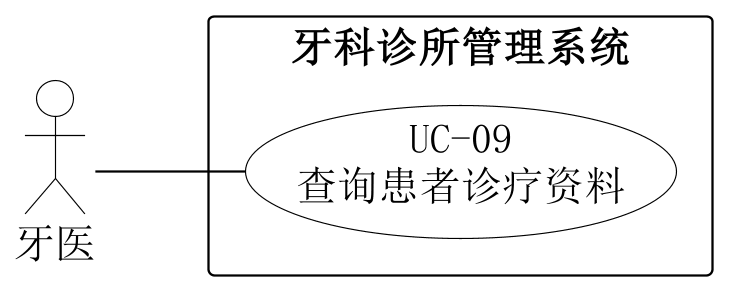
\includegraphics[width=0.90\textwidth,height=2.8cm,keepaspectratio]{diagrams/07-09-system-use-case.png}
\caption{UC-09 查询患者诊疗资料用例图}
\label{fig:uc-09}
\end{figure}
\noindent\textbf{执行者：}牙医

\noindent\textbf{前置条件：}牙医身份有效，具有本人接诊患者诊疗资料的查询权限。

\noindent\textbf{后置条件：}返回选定患者本次就诊及获准的既往病历；不修改临床或收费内容。

\noindent\textbf{涉众利益：}患者希望多次诊疗连续且资料不被无关人员查看；牙医需要掌握病史、过敏及既往治疗。

\noindent\textbf{基本路径}
\begin{enumerate}\setlength{\itemsep}{0pt}
\item 牙医提交本次就诊编号。
\item 系统核对本次接诊归属，反馈患者身份及历次就诊。
\item 牙医选择需要查阅的本次或既往诊疗。
\item 系统反馈病史、检查诊断、方案、治疗经过、诊后要求及补充经历。
\end{enumerate}

\noindent\textbf{扩展路径}

\noindent\textbf{2a 不属于本人接诊范围：}系统拒绝访问，不返回病历正文。

\noindent\textbf{2b 患者没有既往病历：}系统反馈本次资料并说明无既往记录，不将其解释为无病史。

\noindent\textbf{4a 所选病历不可取得：}系统反馈原因，保留查询条件，不以空白内容替代原病历。

\begin{table}[!htbp]
\centering
\caption{UC-09 输入与输出字段}
\label{tab:fields-09}
\small
\renewcommand{\arraystretch}{1.18}
\begin{tabularx}{\textwidth}{@{}>{\raggedright\arraybackslash}p{3.3cm}>{\raggedright\arraybackslash}p{2.0cm}L@{}}
\toprule
字段 & 来源 & 约束及含义 \\
\midrule
本次就诊编号 & 牙医 & 选定唯一就诊，校验接诊归属。 \\
患者身份、历次就诊及日期 & 系统 & 均属于同一患者。 \\
病史、诊断、方案、治疗及补充 & 系统 & 按就诊及时间顺序返回原内容。 \\
\bottomrule
\end{tabularx}
\end{table}

\noindent\textbf{业务规则：}本次接诊牙医可查阅该患者与诊疗有关的既往资料；负责人兼任牙医时仍按接诊关系取得权限。

\noindent\textbf{质量需求：}每次查询校验身份与接诊范围；拒绝时不泄露其他患者正文。

\noindent\textbf{设计约束：}提供工作人员网页查询；不调用影像设备或患者自助接口。

\noindent\textbf{分析序列图：}见图\ref{fig:seq-09}。

\clearpage
\subsubsection{UC-10：记录检查诊断及方案}
\begin{figure}[!htbp]
\centering
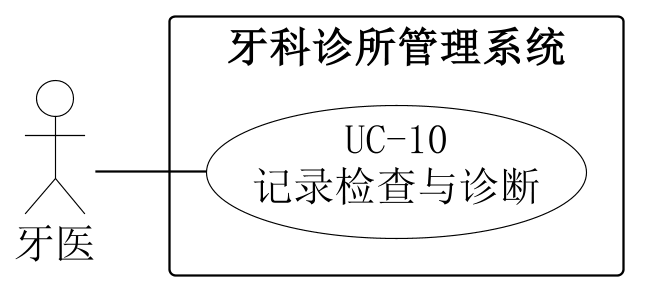
\includegraphics[width=0.90\textwidth,height=2.8cm,keepaspectratio]{diagrams/07-10-system-use-case.png}
\caption{UC-10 记录检查诊断及方案用例图}
\label{fig:uc-10}
\end{figure}
\noindent\textbf{执行者：}牙医

\noindent\textbf{前置条件：}牙医身份有效，具有本人就诊病历编辑权限。

\noindent\textbf{后置条件：}成功时保存本次病史、检查所见、诊断、方案及患者决定；失败时原内容保持不变。

\noindent\textbf{涉众利益：}患者需要理解选择及预计费用；牙医需要完整的临床判断依据；收费人员不能把拟定方案当作实际完成项目。

\noindent\textbf{基本路径}
\begin{enumerate}\setlength{\itemsep}{0pt}
\item 牙医提交本次就诊编号。
\item 系统核对接诊归属，反馈患者、本次病历及已有方案。
\item 牙医提交病史、牙位、检查所见、诊断、治疗方案和患者决定。
\item 系统校验记录完整性、项目及数量，确认病历仍可编辑。
\item 牙医核对记录及已向患者说明的方案，确认提交。
\item 系统再次核对病历和方案，保存临床内容并反馈结果。
\end{enumerate}

\noindent\textbf{扩展路径}

\noindent\textbf{3a 患者尚未决定或仅完成检查：}牙医记录待决定、拒绝或暂缓及说明；系统保留检查结果，不据此产生实际治疗项目。

\noindent\textbf{4a 内容无效或就诊不符：}系统指出问题，牙医核对后返回步骤3。

\noindent\textbf{6a 病历已签署或内容已变化：}系统拒绝覆盖；签署后的说明通过UC-11追加补充。

\begin{table}[!htbp]
\centering
\caption{UC-10 输入与输出字段}
\label{tab:fields-10}
\small
\renewcommand{\arraystretch}{1.18}
\begin{tabularx}{\textwidth}{@{}>{\raggedright\arraybackslash}p{3.3cm}>{\raggedright\arraybackslash}p{2.0cm}L@{}}
\toprule
字段 & 来源 & 约束及含义 \\
\midrule
主诉、相关病史及过敏 & 牙医 & 记录患者陈述；未询明与明确否认应区分。 \\
牙位、检查所见及诊断 & 牙医 & 牙位采用诊所约定表示；全口检查可注明全口。 \\
方案项目、预计数量及费用说明 & 牙医 & 数量为正整数；费用为预计说明，不构成收款。 \\
患者决定及说明时间 & 牙医 & 每个方案项目记录待决定、同意、拒绝或暂缓；记录说明依据。 \\
\bottomrule
\end{tabularx}
\end{table}

\noindent\textbf{业务规则：}诊断和方案由牙医负责；患者决定由牙医如实记录。仅患者同意的方案项目可按方案实施，实际完成项目另由UC-04确认。

\noindent\textbf{质量需求：}方案决定与本次病历、患者一致；失败不留下半套方案或病历。

\noindent\textbf{设计约束：}由牙医记录临床判断，系统不自动生成诊断或代替患者决定。

\noindent\textbf{分析序列图：}见图\ref{fig:seq-10}。

\clearpage
\subsubsection{UC-11：签署及补充病历}
\begin{figure}[!htbp]
\centering
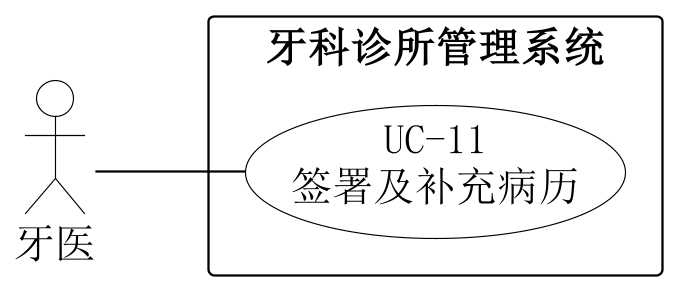
\includegraphics[width=0.90\textwidth,height=2.8cm,keepaspectratio]{diagrams/07-11-system-use-case.png}
\caption{UC-11 签署及补充病历用例图}
\label{fig:uc-11}
\end{figure}
\noindent\textbf{执行者：}牙医

\noindent\textbf{前置条件：}牙医身份有效，具有本人接诊病历的签署权限。

\noindent\textbf{后置条件：}签署后保留签署人、时间及原病历；补充形成独立内容与原因，不覆盖原文。

\noindent\textbf{涉众利益：}患者需要可信的诊疗经过；牙医需要确认诊断、治疗和诊后指导；后续牙医需要区分原文与补充。

\noindent\textbf{基本路径}
\begin{enumerate}\setlength{\itemsep}{0pt}
\item 牙医提交本次病历的签署请求。
\item 系统反馈本次病历及已确认的实际项目。
\item 牙医提交完整的诊疗经过、诊后指导并确认签署。
\item 系统校验接诊归属、必填临床内容及当前病历。
\item 牙医核对待签署内容，确认提交。
\item 系统再次核对并保存签署事实，反馈签署结果。
\end{enumerate}

\noindent\textbf{扩展路径}

\noindent\textbf{1a 已签署病历需要补充：}牙医提交补充内容及原因；系统校验本人权限，追加补充人和时间，保留原文。

\noindent\textbf{4a 主诉、检查诊断或诊后内容缺失：}系统指出缺项，牙医补全后重新提交。

\noindent\textbf{6a 重复签署或原内容变化：}已签署且未变化时返回原签署结果；内容变化时拒绝按旧内容签署。

\begin{table}[!htbp]
\centering
\caption{UC-11 输入与输出字段}
\label{tab:fields-11}
\small
\renewcommand{\arraystretch}{1.18}
\begin{tabularx}{\textwidth}{@{}>{\raggedright\arraybackslash}p{3.3cm}>{\raggedright\arraybackslash}p{2.0cm}L@{}}
\toprule
字段 & 来源 & 约束及含义 \\
\midrule
本次就诊、原病历内容 & 系统／牙医 & 须为本人接诊；签署的是当前完整内容。 \\
签署人及时间 & 系统 & 随签署保存；助理与前台不得代签。 \\
补充内容、原因及时间 & 牙医／系统 & 补充内容及原因必填，与原病历关联。 \\
\bottomrule
\end{tabularx}
\end{table}

\noindent\textbf{业务规则：}签署后不得编辑原病历正文；补充不撤销签署、不改写已结清的收费依据。实际项目更正按UC-04办理。

\noindent\textbf{质量需求：}签署失败保留原稿；成功后正文及补充均可按时间回查。

\noindent\textbf{设计约束：}工作人员网页记录签署确认；不引入外部电子签章服务。

\noindent\textbf{分析序列图：}签署见图\ref{fig:seq-11}，补充见图\ref{fig:seq-11-ext}。

\clearpage
\subsubsection{UC-12：提出复诊随访要求}
\begin{figure}[!htbp]
\centering
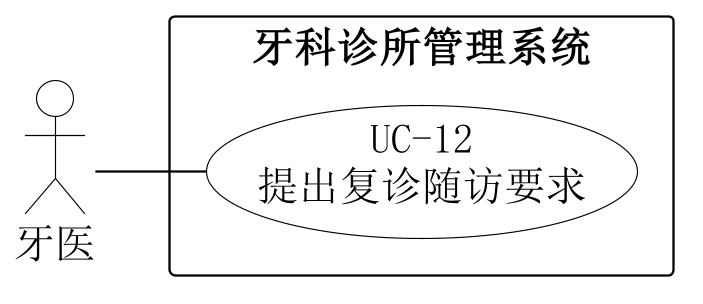
\includegraphics[width=0.90\textwidth,height=2.8cm,keepaspectratio]{diagrams/07-12-system-use-case.png}
\caption{UC-12 提出复诊随访要求用例图}
\label{fig:uc-12}
\end{figure}
\noindent\textbf{执行者：}牙医

\noindent\textbf{前置条件：}牙医身份有效，具有本人已签署就诊的诊后要求维护权限。

\noindent\textbf{后置条件：}保存与来源就诊、患者关联的诊后要求、负责前台及目标日期；生成待联系事项。

\noindent\textbf{涉众利益：}患者需要清楚的后续诊疗安排；前台需要明确联系依据；复诊牙医需要查明前次诊疗来源。

\noindent\textbf{基本路径}
\begin{enumerate}\setlength{\itemsep}{0pt}
\item 牙医提交来源就诊编号及诊后要求请求。
\item 系统反馈来源病历、患者及已有诊后要求。
\item 牙医提交复诊或随访目的、目标日期、注意事项及负责前台。
\item 系统核对来源、患者及人员，校验要求与日期。
\item 牙医核对要求并确认提交。
\item 系统保存要求及提出人、时间，反馈待联系结果。
\end{enumerate}

\noindent\textbf{扩展路径}

\noindent\textbf{2a 来源未签署或不属于本人：}系统拒绝建立要求，牙医核对或完成UC-11后重试。

\noindent\textbf{4a 无目的、日期或有效前台：}系统指出问题，牙医补全后返回步骤3。

\noindent\textbf{6a 重复的同一提交：}系统返回既有要求，不重复产生待办。

\begin{table}[!htbp]
\centering
\caption{UC-12 输入与输出字段}
\label{tab:fields-12}
\small
\renewcommand{\arraystretch}{1.18}
\begin{tabularx}{\textwidth}{@{}>{\raggedright\arraybackslash}p{3.3cm}>{\raggedright\arraybackslash}p{2.0cm}L@{}}
\toprule
字段 & 来源 & 约束及含义 \\
\midrule
来源就诊及患者 & 系统／牙医 & 必须属于同一患者和本人已签署就诊。 \\
要求类型、目的、目标日期 & 牙医 & 类型为复诊或随访；目的和目标日期必填。 \\
负责前台、提出人及时间 & 牙医／系统 & 前台须为有效人员；记录实际提出人。 \\
\bottomrule
\end{tabularx}
\end{table}

\noindent\textbf{业务规则：}目标日期表达牙医的诊后安排，不自动占用预约时段；需要到诊时仍通过UC-01办理预约。

\noindent\textbf{质量需求：}要求与来源就诊同时关联；重复提交不增加重复联系事项。

\noindent\textbf{设计约束：}联系患者由前台实际办理，本用例不发送模拟或真实消息。

\noindent\textbf{分析序列图：}见图\ref{fig:seq-12}。

\clearpage
\subsubsection{UC-13：办理复诊随访联系}
\begin{figure}[!htbp]
\centering
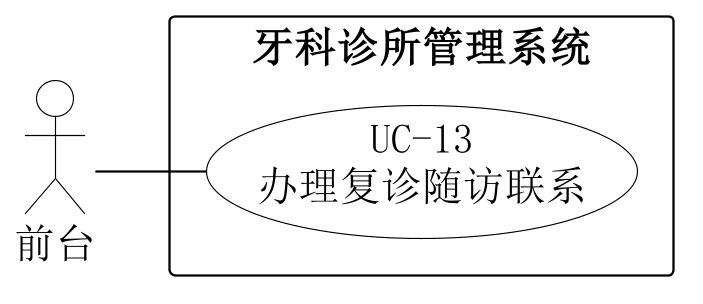
\includegraphics[width=0.90\textwidth,height=2.8cm,keepaspectratio]{diagrams/07-13-system-use-case.png}
\caption{UC-13 办理复诊随访联系用例图}
\label{fig:uc-13}
\end{figure}
\noindent\textbf{执行者：}前台

\noindent\textbf{前置条件：}前台身份有效，具有诊后联系办理权限。

\noindent\textbf{后置条件：}保存每次联系结果、经办人及时间；必要时保存下次联系日期或同患者复诊预约关联。

\noindent\textbf{涉众利益：}患者希望安排准确且不重复联系；前台需要可追溯的反馈；牙医需要了解诊后执行情况。

\noindent\textbf{基本路径}
\begin{enumerate}\setlength{\itemsep}{0pt}
\item 前台提交目标日期或患者等待联系查询条件。
\item 系统反馈诊后要求、来源就诊及已有联系经历。
\item 前台提交实际联系时间、反馈、后续办理选择及说明。
\item 系统校验要求仍可办理，核对日期与复诊预约归属。
\item 前台核对联系记录及后续安排，确认提交。
\item 系统追加联系经历，更新办理结果并反馈。
\end{enumerate}

\noindent\textbf{扩展路径}

\noindent\textbf{3a 未联系成功：}前台提交原因及下次联系日期；系统保持待联系并追加经历。

\noindent\textbf{3b 患者同意复诊：}前台通过UC-01建立预约，再提交该预约；系统校验同患者、非来源预约且未取消后关联。

\noindent\textbf{2a 关联复诊预约已取消：}系统展示原预约及取消依据，要求保持待联系；前台重新联系，需要复诊时按3b关联新预约。原联系及预约经历保留。

\noindent\textbf{3c 患者取消后续安排：}前台提交原因；系统保留要求和经历，记录取消结果。

\noindent\textbf{4a 要求已完成、预约不符或日期缺失：}系统拒绝更改，反馈具体原因。

\noindent\textbf{6a 内容已被他人办理：}系统反馈最新结果，拒绝覆盖。

\begin{table}[!htbp]
\centering
\caption{UC-13 输入与输出字段}
\label{tab:fields-13}
\small
\renewcommand{\arraystretch}{1.18}
\begin{tabularx}{\textwidth}{@{}>{\raggedright\arraybackslash}p{3.3cm}>{\raggedright\arraybackslash}p{2.0cm}L@{}}
\toprule
字段 & 来源 & 约束及含义 \\
\midrule
诊后要求、来源就诊 & 系统 & 用于定位患者及临床安排。 \\
联系时间、反馈及经办前台 & 前台／系统 & 逐次保存，不能覆盖既有经历。 \\
办理选择、下次联系日期、预约 & 前台 & 未接通须下次日期；已约复诊须同患者有效预约。 \\
取消原因 & 前台 & 取消时必填。 \\
\bottomrule
\end{tabularx}
\end{table}

\noindent\textbf{业务规则：}已联系不等于完成临床评估。前台不能替牙医记录评估完成；同一要求关联的预约与来源预约不同。UC-01取消其当前复诊预约时，未完成的要求返回待联系；仅取消预约不终结诊后要求，也不记为联系成功。

\noindent\textbf{质量需求：}重复提交同一次联系不重复追加；办理与联系经历同时保存。

\noindent\textbf{设计约束：}前台实际联系患者并记录结果，系统不代替电话或面对面沟通。

\noindent\textbf{分析序列图：}见图\ref{fig:seq-13}。

\clearpage
\subsubsection{UC-14：记录复诊随访评估}
\begin{figure}[!htbp]
\centering
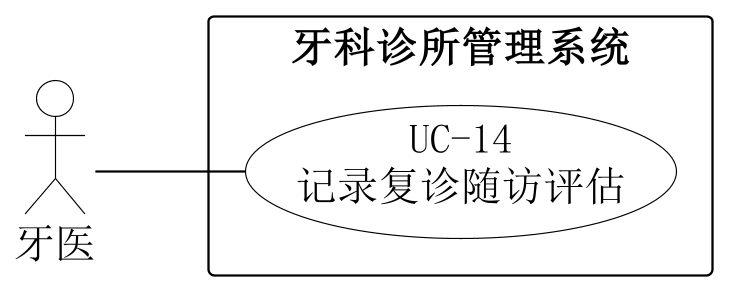
\includegraphics[width=0.90\textwidth,height=2.8cm,keepaspectratio]{diagrams/07-14-system-use-case.png}
\caption{UC-14 记录复诊随访评估用例图}
\label{fig:uc-14}
\end{figure}
\noindent\textbf{执行者：}牙医

\noindent\textbf{前置条件：}牙医身份有效，具有来源就诊或关联复诊的接诊权限。

\noindent\textbf{后置条件：}保存临床评估、处理意见及评估人、时间；要求进入评估完成，原联系和来源资料保留。

\noindent\textbf{涉众利益：}患者希望后续诊疗有明确结论；牙医需要区分联系完成与临床完成；前台需要可靠的关闭依据。

\noindent\textbf{基本路径}
\begin{enumerate}\setlength{\itemsep}{0pt}
\item 牙医提交待评估的诊后要求。
\item 系统反馈来源病历、联系经历及关联复诊病历。
\item 牙医提交实际恢复情况、评估结论与后续处理意见。
\item 系统核对接诊权限、评估内容及复诊病历确认情况。
\item 牙医核对评估内容，确认提交。
\item 系统保存评估及经办时间，反馈评估完成。
\end{enumerate}

\noindent\textbf{扩展路径}

\noindent\textbf{2a 要求已取消或已完成：}系统反馈已有结果，不覆盖终结内容。

\noindent\textbf{4a 预约复诊尚无已签署病历：}系统拒绝完成评估，牙医先办理本次诊疗及UC-11。

\noindent\textbf{4b 无权限或评估内容缺失：}系统反馈原因，牙医补全或交接诊牙医办理。

\noindent\textbf{6a 重复确认同一评估：}系统返回原评估，不增加重复结果。

\begin{table}[!htbp]
\centering
\caption{UC-14 输入与输出字段}
\label{tab:fields-14}
\small
\renewcommand{\arraystretch}{1.18}
\begin{tabularx}{\textwidth}{@{}>{\raggedright\arraybackslash}p{3.3cm}>{\raggedright\arraybackslash}p{2.0cm}L@{}}
\toprule
字段 & 来源 & 约束及含义 \\
\midrule
要求、来源及复诊就诊 & 系统 & 来源与关联复诊必须属于同患者。 \\
恢复情况、结论及处理意见 & 牙医 & 实际评估内容必填。 \\
评估牙医、完成时间 & 系统 & 须为来源或复诊的接诊牙医。 \\
\bottomrule
\end{tabularx}
\end{table}

\noindent\textbf{业务规则：}联系反馈不能替代临床评估。已约复诊的要求须有对应已签署病历；纯随访按实际获知情况记录评估，不伪造到诊。

\noindent\textbf{质量需求：}评估与完成结果同时生效，失败不关闭待办。

\noindent\textbf{设计约束：}系统保存牙医判断；需再次到诊时另提出要求并办理预约。

\noindent\textbf{分析序列图：}见图\ref{fig:seq-14}。

\clearpage
\subsubsection{UC-15：维护接诊人员安排}
\begin{figure}[!htbp]
\centering
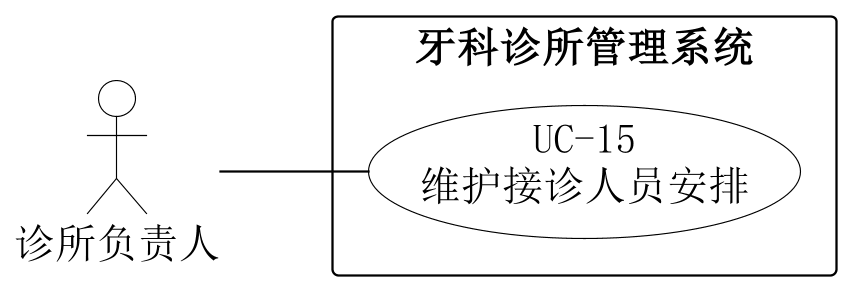
\includegraphics[width=0.90\textwidth,height=2.8cm,keepaspectratio]{diagrams/07-15-system-use-case.png}
\caption{UC-15 维护接诊人员安排用例图}
\label{fig:uc-15}
\end{figure}
\noindent\textbf{执行者：}诊所负责人

\noindent\textbf{前置条件：}负责人身份有效，具有人员接诊安排维护权限。

\noindent\textbf{后置条件：}保存经确认的接诊时段及经办人、时间；有效预约继续获得人员时段支持；失败保留原安排。

\noindent\textbf{涉众利益：}患者希望既有预约可靠；牙医希望时段符合实际出诊；前台需要一致的可接诊依据。

\noindent\textbf{基本路径}
\begin{enumerate}\setlength{\itemsep}{0pt}
\item 诊所负责人提交待维护人员及期间。
\item 系统反馈人员、已有接诊时段及受影响预约。
\item 诊所负责人提交经牙医确认的接诊时段及变更原因。
\item 系统校验人员有效、时段合法且与有效预约相容。
\item 诊所负责人核对安排，确认发布。
\item 系统再次检查相关预约，保存已确认时段并反馈有效安排。
\end{enumerate}

\noindent\textbf{扩展路径}

\noindent\textbf{4a 新安排不能覆盖有效预约：}系统列出受影响时段，不保存变更；相关岗位先通过UC-01协调预约后重新提交。

\noindent\textbf{4b 人员无效或时段重复：}系统指出问题，负责人修正后返回步骤3。

\noindent\textbf{6a 期间预约或安排已变化：}系统拒绝按旧依据发布，反馈最新内容。

\begin{table}[!htbp]
\centering
\caption{UC-15 输入与输出字段}
\label{tab:fields-15}
\small
\renewcommand{\arraystretch}{1.18}
\begin{tabularx}{\textwidth}{@{}>{\raggedright\arraybackslash}p{3.3cm}>{\raggedright\arraybackslash}p{2.0cm}L@{}}
\toprule
字段 & 来源 & 约束及含义 \\
\midrule
接诊牙医、适用星期 & 负责人 & 牙医须有效；说明每周的可接诊日。 \\
起止时间、确认依据 & 负责人 & 结束晚于开始；保存接诊牙医的确认人、确认时间及核实内容，供时段内预约引用。 \\
变更原因、发布人及时间 & 负责人／系统 & 变更须原因；保留原安排。 \\
\bottomrule
\end{tabularx}
\end{table}

\noindent\textbf{业务规则：}有效接诊安排与预约使用同一时段口径，负责人发布前保存牙医确认依据；该时段内预约可引用此依据。时段改变须重新获得牙医确认，不得用停用人员或缩短时段静默失效已有预约。

\noindent\textbf{质量需求：}预约改变与安排发布并行时仍须复核，不得产生无接诊支持的有效预约。

\noindent\textbf{设计约束：}负责人使用网页记录已确认安排，系统不自动决定人员出诊。

\noindent\textbf{分析序列图：}见图\ref{fig:seq-15}。

\clearpage
\subsubsection{UC-16：查询可用接诊安排}
\begin{figure}[!htbp]
\centering
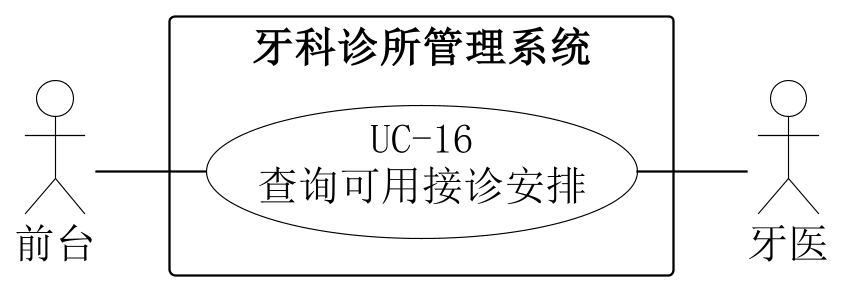
\includegraphics[width=0.90\textwidth,height=2.8cm,keepaspectratio]{diagrams/07-16-system-use-case.png}
\caption{UC-16 查询可用接诊安排用例图}
\label{fig:uc-16}
\end{figure}
\noindent\textbf{执行者：}前台、牙医

\noindent\textbf{前置条件：}操作者身份有效，具有接诊安排查询权限。

\noindent\textbf{后置条件：}返回所选日期的有效人员时段、已占用时间及可预约安排；查询不建立预约。

\noindent\textbf{涉众利益：}前台需要可协商的时间；患者希望约定可执行；牙医需要查看本人接诊安排。

\noindent\textbf{基本路径}
\begin{enumerate}\setlength{\itemsep}{0pt}
\item 前台或牙医提交日期、牙医及查询时段。
\item 系统校验条件和人员范围，核对已发布时段及有效预约。
\item 系统反馈已确认时段、占用时间及可用安排。
\item 前台或牙医选择需要核对的安排，系统反馈当前详情。
\end{enumerate}

\noindent\textbf{扩展路径}

\noindent\textbf{2a 日期或人员条件无效：}系统反馈原因，不返回伪造的可用时段。

\noindent\textbf{3a 没有可接诊安排：}系统说明无可用安排，前台与相关人员协调后重新查询。

\noindent\textbf{4a 详情已变化：}系统返回当前结果；新增预约仍由UC-01再次校验。

\begin{table}[!htbp]
\centering
\caption{UC-16 输入与输出字段}
\label{tab:fields-16}
\small
\renewcommand{\arraystretch}{1.18}
\begin{tabularx}{\textwidth}{@{}>{\raggedright\arraybackslash}p{3.3cm}>{\raggedright\arraybackslash}p{2.0cm}L@{}}
\toprule
字段 & 来源 & 约束及含义 \\
\midrule
日期、牙医、所需时长 & 执行者 & 日期及有效人员为查询依据；时长须为正值。 \\
接诊时段、占用及可用安排 & 系统 & 采用相同时间口径；牙医仅查询其获准范围。 \\
\bottomrule
\end{tabularx}
\end{table}

\noindent\textbf{业务规则：}结束时点等于下一时段开始时点不视为重叠；查询结果不能作为绕过最终冲突检查的许可。

\noindent\textbf{质量需求：}不向无关人员返回其他患者姓名及联系方式；无结果与查询失败分别反馈。

\noindent\textbf{设计约束：}通过工作人员网页查询。

\noindent\textbf{分析序列图：}见图\ref{fig:seq-16}。

\clearpage
\subsubsection{UC-17：查询材料库存}
\begin{figure}[!htbp]
\centering
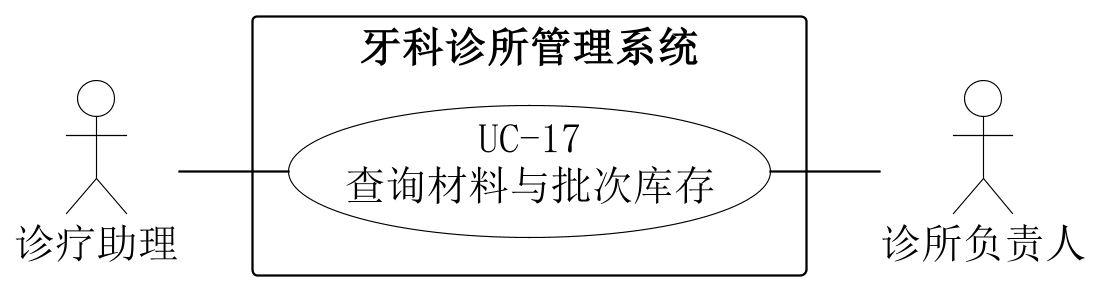
\includegraphics[width=0.90\textwidth,height=2.8cm,keepaspectratio]{diagrams/07-17-system-use-case.png}
\caption{UC-17 查询材料库存用例图}
\label{fig:uc-17}
\end{figure}
\noindent\textbf{执行者：}诊疗助理、诊所负责人

\noindent\textbf{前置条件：}操作者身份有效，具有材料查询权限。

\noindent\textbf{后置条件：}返回材料、计量单位、账面数量及收发盘点经历；不改变库存。

\noindent\textbf{涉众利益：}助理需要判断可用数量；负责人需要核对补充及差异；牙医需要实际材料保障。

\noindent\textbf{基本路径}
\begin{enumerate}\setlength{\itemsep}{0pt}
\item 诊疗助理或诊所负责人提交材料或期间条件。
\item 系统校验查询范围，查得材料及对应变动。
\item 系统反馈计量单位、账面库存及原始变动经历。
\item 执行者选择需核对的变动，系统反馈前后数量、经办及确认依据。
\end{enumerate}

\noindent\textbf{扩展路径}

\noindent\textbf{2a 材料不存在或条件无效：}系统说明问题，不将查不到解释为零库存。

\noindent\textbf{3a 没有期间变动：}系统说明无变动，仍返回当前账面数量。

\begin{table}[!htbp]
\centering
\caption{UC-17 输入与输出字段}
\label{tab:fields-17}
\small
\renewcommand{\arraystretch}{1.18}
\begin{tabularx}{\textwidth}{@{}>{\raggedright\arraybackslash}p{3.3cm}>{\raggedright\arraybackslash}p{2.0cm}L@{}}
\toprule
字段 & 来源 & 约束及含义 \\
\midrule
材料名称及期间 & 执行者 & 期间结束不得早于开始。 \\
单位、账面数量、变动前后数量 & 系统 & 采用材料的同一计量单位。 \\
用途、经办人、时间及确认依据 & 系统 & 返回原始经历，不以当前余额替代历史。 \\
\bottomrule
\end{tabularx}
\end{table}

\noindent\textbf{业务规则：}账面库存与实物库存需要由助理实际核对；库存不足可向负责人报告，查询不自动形成采购。

\noindent\textbf{质量需求：}查询失败不返回零库存；所有显示数量与保存的变动一致。

\noindent\textbf{设计约束：}提供材料台账查询，不连接采购或仓储外系统。

\noindent\textbf{分析序列图：}见图\ref{fig:seq-17}。

\clearpage
\subsubsection{UC-18：登记材料变动}
\begin{figure}[!htbp]
\centering
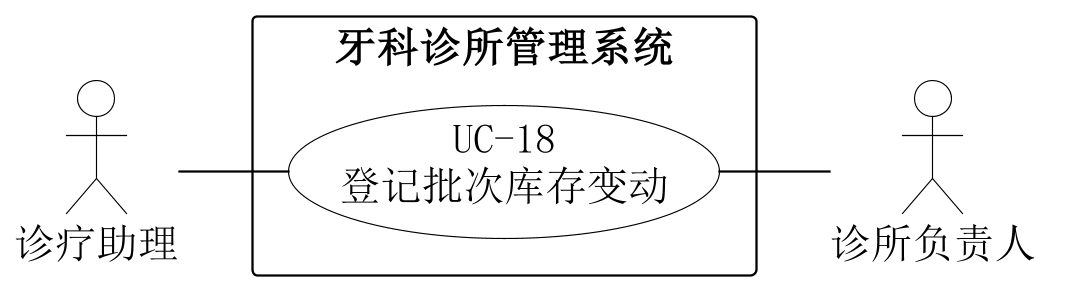
\includegraphics[width=0.90\textwidth,height=2.8cm,keepaspectratio]{diagrams/07-18-system-use-case.png}
\caption{UC-18 登记材料变动用例图}
\label{fig:uc-18}
\end{figure}
\noindent\textbf{执行者：}诊疗助理

\noindent\textbf{前置条件：}助理身份有效，具有材料收发与盘点登记权限。

\noindent\textbf{后置条件：}成功时保留原始变动、前后数量和经办依据并更新库存；失败不改变余额或留下部分变动。

\noindent\textbf{涉众利益：}助理需要收发与实物一致；负责人需要可追溯的盘点差异；牙医需要可用诊疗材料。

\noindent\textbf{基本路径}
\begin{enumerate}\setlength{\itemsep}{0pt}
\item 诊疗助理提交材料及变动类型。
\item 系统反馈材料单位、账面数量及需要提交的依据。
\item 诊疗助理提交实际入库、领用数量或实盘数量，以及用途或原因。
\item 系统校验材料、数量、库存及盘点确认依据。
\item 诊疗助理核对变动内容，确认提交。
\item 系统再次核对库存，保存变动与余额，反馈当前库存。
\end{enumerate}

\noindent\textbf{扩展路径}

\noindent\textbf{3a 登记盘点调整：}助理提交实盘数量、差异原因及负责人确认人、时间和意见；系统核对后按实盘数调整。

\noindent\textbf{4a 领用超过可用库存：}系统拒绝领用，反馈可用数量，不扣库。

\noindent\textbf{4b 材料无效、数量非法或确认缺失：}系统说明原因，助理核实后返回步骤3。

\noindent\textbf{6a 库存已变化：}系统重新校验，无法满足领用时拒绝，不覆盖原始流水。

\begin{table}[!htbp]
\centering
\caption{UC-18 输入与输出字段}
\label{tab:fields-18}
\small
\renewcommand{\arraystretch}{1.18}
\begin{tabularx}{\textwidth}{@{}>{\raggedright\arraybackslash}p{3.3cm}>{\raggedright\arraybackslash}p{2.0cm}L@{}}
\toprule
字段 & 来源 & 约束及含义 \\
\midrule
材料、变动类型、单位 & 助理／系统 & 材料须有效；类型为入库、领用或盘点调整。 \\
入库或领用数量、实盘数量 & 助理 & 收发数量大于零；实盘数量不少于零，均为有限数值。 \\
用途／原因、经办及时间 & 助理／系统 & 用途或原因必填；保留变动前后数量。 \\
负责人确认信息 & 助理 & 盘点调整必填，确认人员有效且时间不得在未来。 \\
\bottomrule
\end{tabularx}
\end{table}

\noindent\textbf{业务规则：}入库增加库存，领用减少库存，盘点按负责人确认的实盘数量调整；账面余额不得为负。原始变动不得覆盖或删除。

\noindent\textbf{质量需求：}库存与变动同时生效，失败两者均保持原结果；重复提交不重复扣库。

\noindent\textbf{设计约束：}实际清点、发放、器械清洁消毒由助理执行；本用例只记录材料变动。

\noindent\textbf{分析序列图：}见图\ref{fig:seq-18}。

\clearpage
\subsubsection{UC-19：查询日常业务与收款}
\begin{figure}[!htbp]
\centering
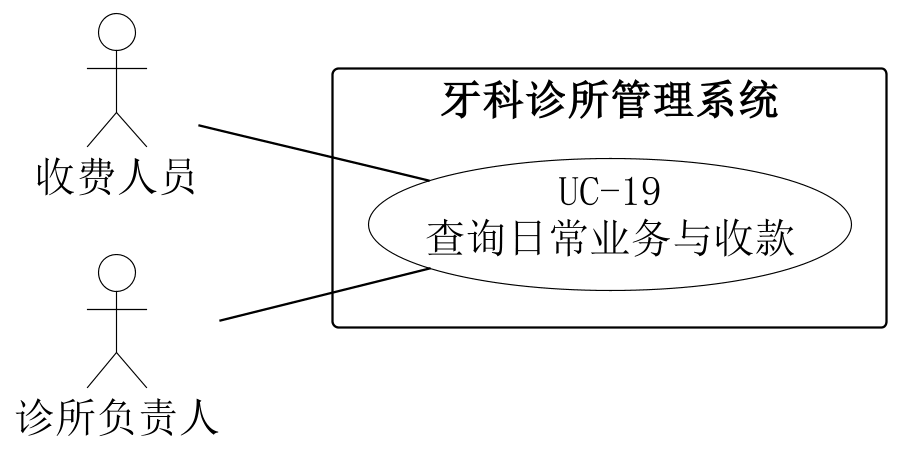
\includegraphics[width=0.90\textwidth,height=2.8cm,keepaspectratio]{diagrams/07-19-system-use-case.png}
\caption{UC-19 查询日常业务与收款用例图}
\label{fig:uc-19}
\end{figure}
\noindent\textbf{执行者：}收费人员、诊所负责人

\noindent\textbf{前置条件：}操作者身份有效，具有对应业务或收款统计查询权限。

\noindent\textbf{后置条件：}返回同期间获准的就诊、实际项目、有效现金收款及未结清明细；不改变原业务。

\noindent\textbf{涉众利益：}负责人需要可信的运行情况；收费人员需要与现金及收据核对；患者的临床正文应限制在诊疗范围。

\noindent\textbf{基本路径}
\begin{enumerate}\setlength{\itemsep}{0pt}
\item 收费人员或诊所负责人提交统计起止日期及业务条件。
\item 系统核对日期与查询权限，定位同期间的业务。
\item 系统按各自发生日期汇总就诊、实际项目、有效现金净收及未结清情况。
\item 系统反馈统计口径、汇总及可核对的明细。
\end{enumerate}

\noindent\textbf{扩展路径}

\noindent\textbf{2a 日期非法或范围无权：}系统反馈原因，不返回越权内容。

\noindent\textbf{3a 没有相关业务：}系统反馈零数量及空明细，并说明统计期间；失败不得当作零。

\noindent\textbf{4a 需要核对差异：}执行者选择原始明细核实，收款核对另由UC-20办理。

\begin{table}[!htbp]
\centering
\caption{UC-19 输入与输出字段}
\label{tab:fields-19}
\small
\renewcommand{\arraystretch}{1.18}
\begin{tabularx}{\textwidth}{@{}>{\raggedright\arraybackslash}p{3.3cm}>{\raggedright\arraybackslash}p{2.0cm}L@{}}
\toprule
字段 & 来源 & 约束及含义 \\
\midrule
起止日期、统计条件 & 执行者 & 结束不得早于开始；使用诊所当地日期。 \\
就诊人次、实际项目及未结清 & 系统 & 就诊按到诊日期；实际项目按UC-04记录的完成时间取当地日期，仅统计当前有效版本，不按补录或更正确认日重复计数。 \\
现金收款、找零及净收 & 系统 & 按实际收款日期；净收为实收扣除找零。 \\
明细及对应凭据 & 系统 & 可回查各项汇总的来源。 \\
\bottomrule
\end{tabularx}
\end{table}

\noindent\textbf{业务规则：}收入汇总不表示利润；方案预计项目不得算作已完成项目，账单应收不得算作已收现金。收费人员只查询收款核对所需范围。

\noindent\textbf{质量需求：}相同条件汇总与明细一致，金额精确到分；查询不改变任何凭据。

\noindent\textbf{设计约束：}通过网页查询业务及收款统计。

\noindent\textbf{分析序列图：}见图\ref{fig:seq-19}。

\clearpage
\subsubsection{UC-20：登记收款核对}
\begin{figure}[!htbp]
\centering
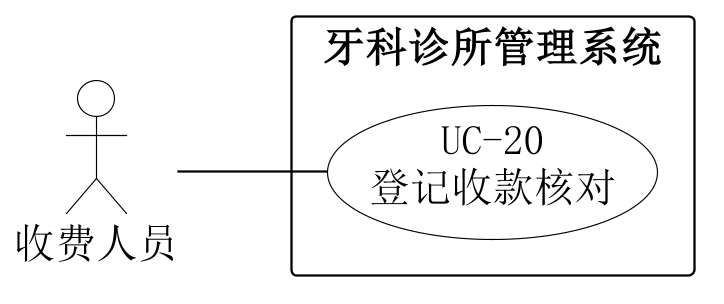
\includegraphics[width=0.90\textwidth,height=2.8cm,keepaspectratio]{diagrams/07-20-system-use-case.png}
\caption{UC-20 登记收款核对用例图}
\label{fig:uc-20}
\end{figure}
\noindent\textbf{执行者：}收费人员

\noindent\textbf{前置条件：}收费人员身份有效，具有日常现金核对登记权限。

\noindent\textbf{后置条件：}保存核对日、统计依据、实际盘点、差异及处理意见和经办时间；不改写原现金收款。

\noindent\textbf{涉众利益：}收费人员希望现金、收据和汇总一致；负责人需要明确差异和处理依据；患者的原收据应保留。

\noindent\textbf{基本路径}
\begin{enumerate}\setlength{\itemsep}{0pt}
\item 收费人员提交需要核对的营业日期。
\item 系统反馈该日有效收款、现金净收及已有核对经历。
\item 收费人员提交扣除开班现金后的实际收款盘点金额及差异说明、处理意见。
\item 系统核验金额和说明，计算盘点与有效现金净收的差额。
\item 收费人员核对结果；存在差异时提交负责人已确认的处理依据并确认登记。
\item 系统再次核对统计依据，保存核对经历并反馈结果。
\end{enumerate}

\noindent\textbf{扩展路径}

\noindent\textbf{4a 盘点金额不合法或差异说明缺失：}系统指出问题，收费人员实际复核后返回步骤3。

\noindent\textbf{5a 尚未确定差异原因及处理意见：}系统保留原核对，收费人员核实并取得负责人意见后重新提交。

\noindent\textbf{6a 该日收款明细已变化：}系统反馈最新汇总，拒绝沿用旧核对依据。

\noindent\textbf{6b 重复提交同一次核对：}系统返回原核对结果，不改变任何原收据。

\begin{table}[!htbp]
\centering
\caption{UC-20 输入与输出字段}
\label{tab:fields-20}
\small
\renewcommand{\arraystretch}{1.18}
\begin{tabularx}{\textwidth}{@{}>{\raggedright\arraybackslash}p{3.3cm}>{\raggedright\arraybackslash}p{2.0cm}L@{}}
\toprule
字段 & 来源 & 约束及含义 \\
\midrule
核对日期及有效收款依据 & 系统／收费人员 & 统一当地营业日；对应可查询的原收据。 \\
盘点净收金额、差额 & 收费人员／系统 & 精确到分；盘点扣除开班现金，不将找零重复扣除。 \\
差异原因、负责人处理意见 & 收费人员 & 差异非零时必填，记录确认依据。 \\
经办人、核对时间、原核对经历 & 系统 & 追加保留，不能覆盖原凭据。 \\
\bottomrule
\end{tabularx}
\end{table}

\noindent\textbf{业务规则：}差额为盘点净收减系统现金净收。核对说明不能用于改写收据或补造收款；业务更正交对应岗位按原用例办理。

\noindent\textbf{质量需求：}核对保存失败不改变收款；依据变化须重新核对；保留每次原始经历。

\noindent\textbf{设计约束：}实际清点现金及负责人处理确认由工作人员执行。

\noindent\textbf{分析序列图：}见图\ref{fig:seq-20}。

\clearpage
\endgroup
\section{分析}
本章按照第二章的系统用例分配边界、控制及实体责任，分析核心业务对象之间的协作及生命周期。

\subsection{分析类图}
\subsubsection{边界类与控制类}

根据五类系统执行者设置前台接口、牙医接口、收费人员接口、诊疗助理接口和诊所负责人接口，负责接收输入、基本格式检查及展示结果。每个系统用例对应一个控制类，按规约协调处理顺序，并将业务判断交给相应实体。

\begin{figure}[htbp]
\centering
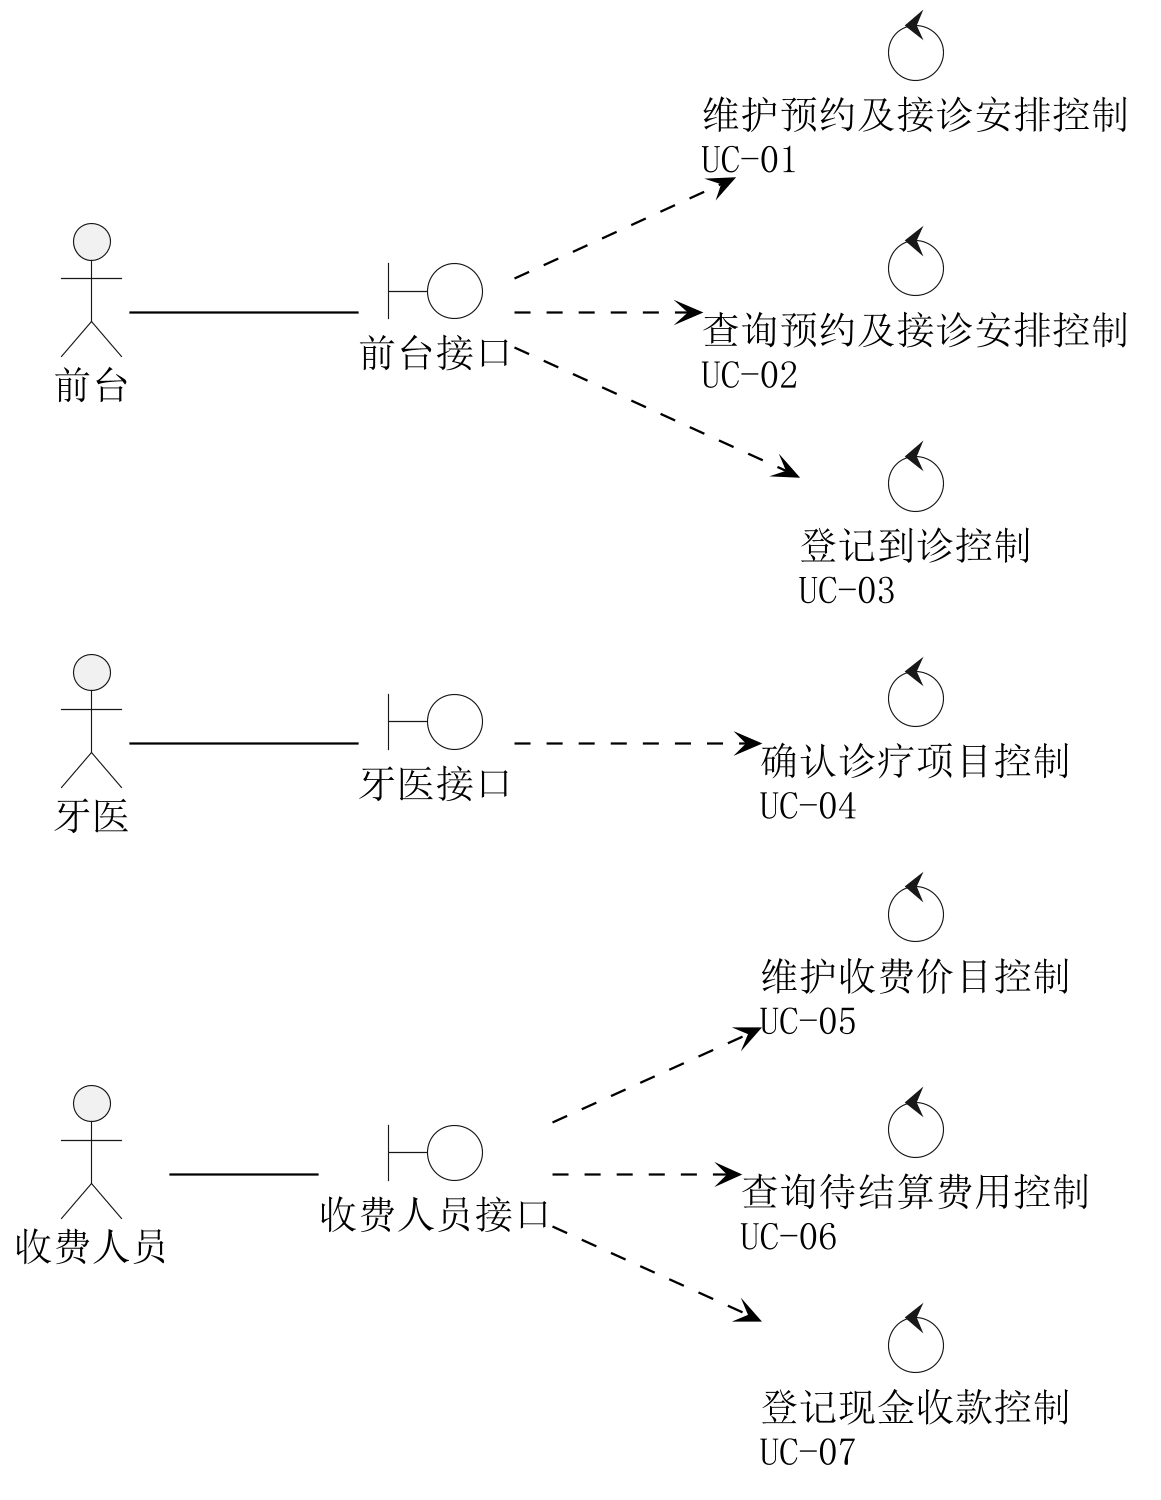
\includegraphics[width=\textwidth,height=16.3cm,keepaspectratio]{diagrams/10-analysis-boundary-control.png}
\caption{分析类图：预约接待与收费的边界类及控制类}
\label{fig:analysis-bc}
\end{figure}


\clearpage
\clearpage
\begin{figure}[!htbp]
\centering
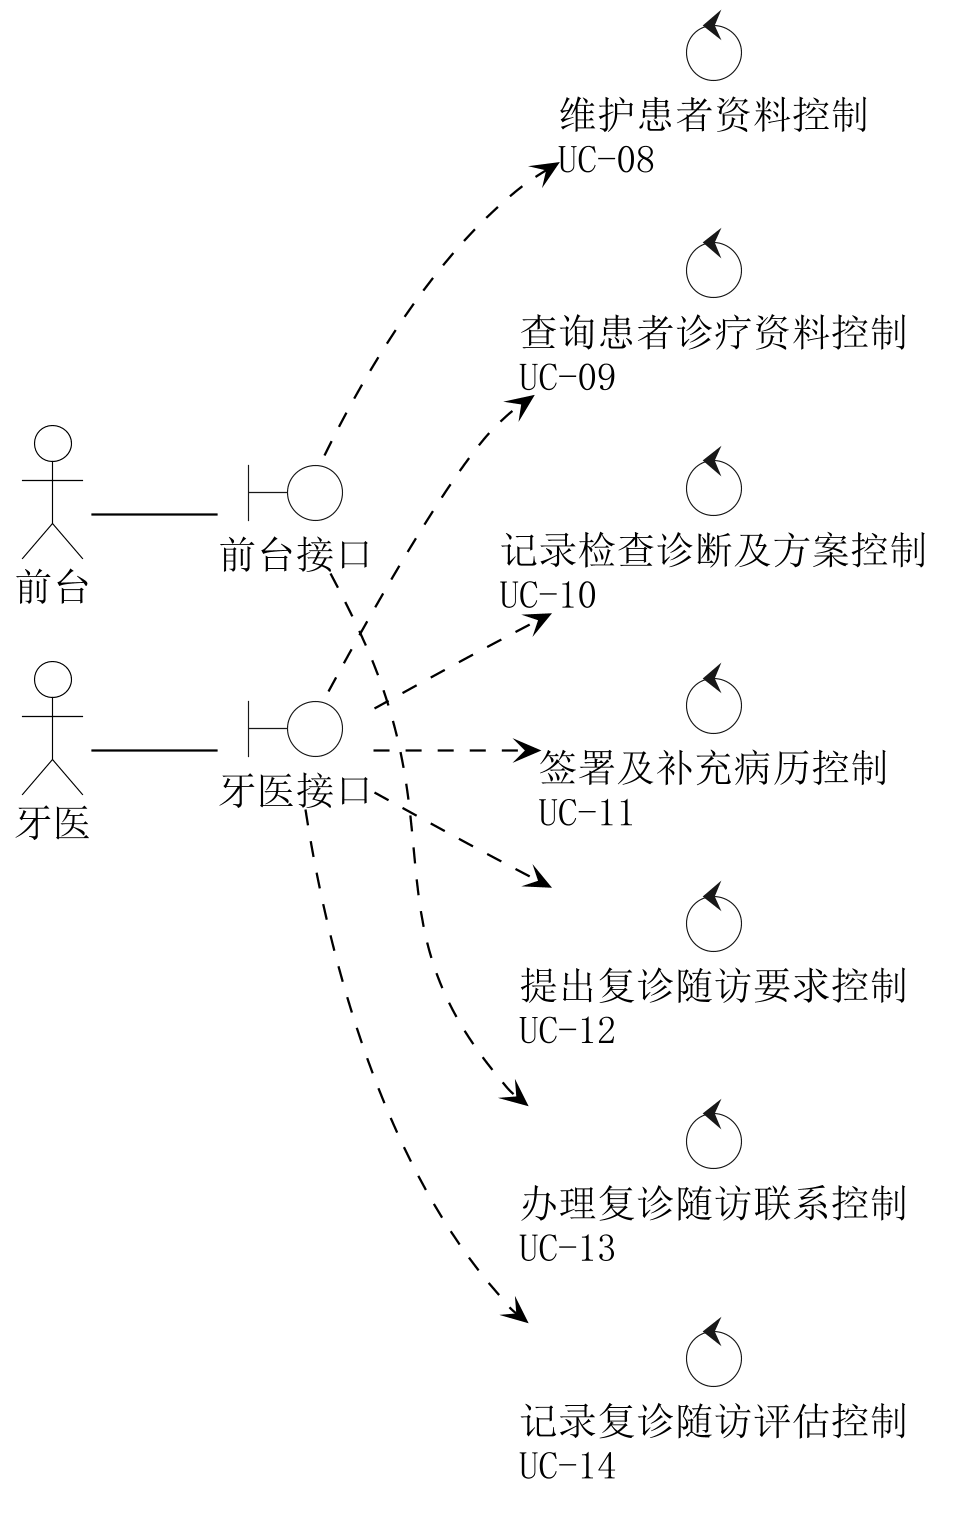
\includegraphics[width=\textwidth,height=19cm,keepaspectratio]{diagrams/10a-analysis-clinical-boundary-control.png}
\caption{分析类图：患者资料、病历与复诊的边界类及控制类}
\label{fig:analysis-bc-clinical}
\end{figure}
\clearpage
\begin{figure}[!htbp]
\centering
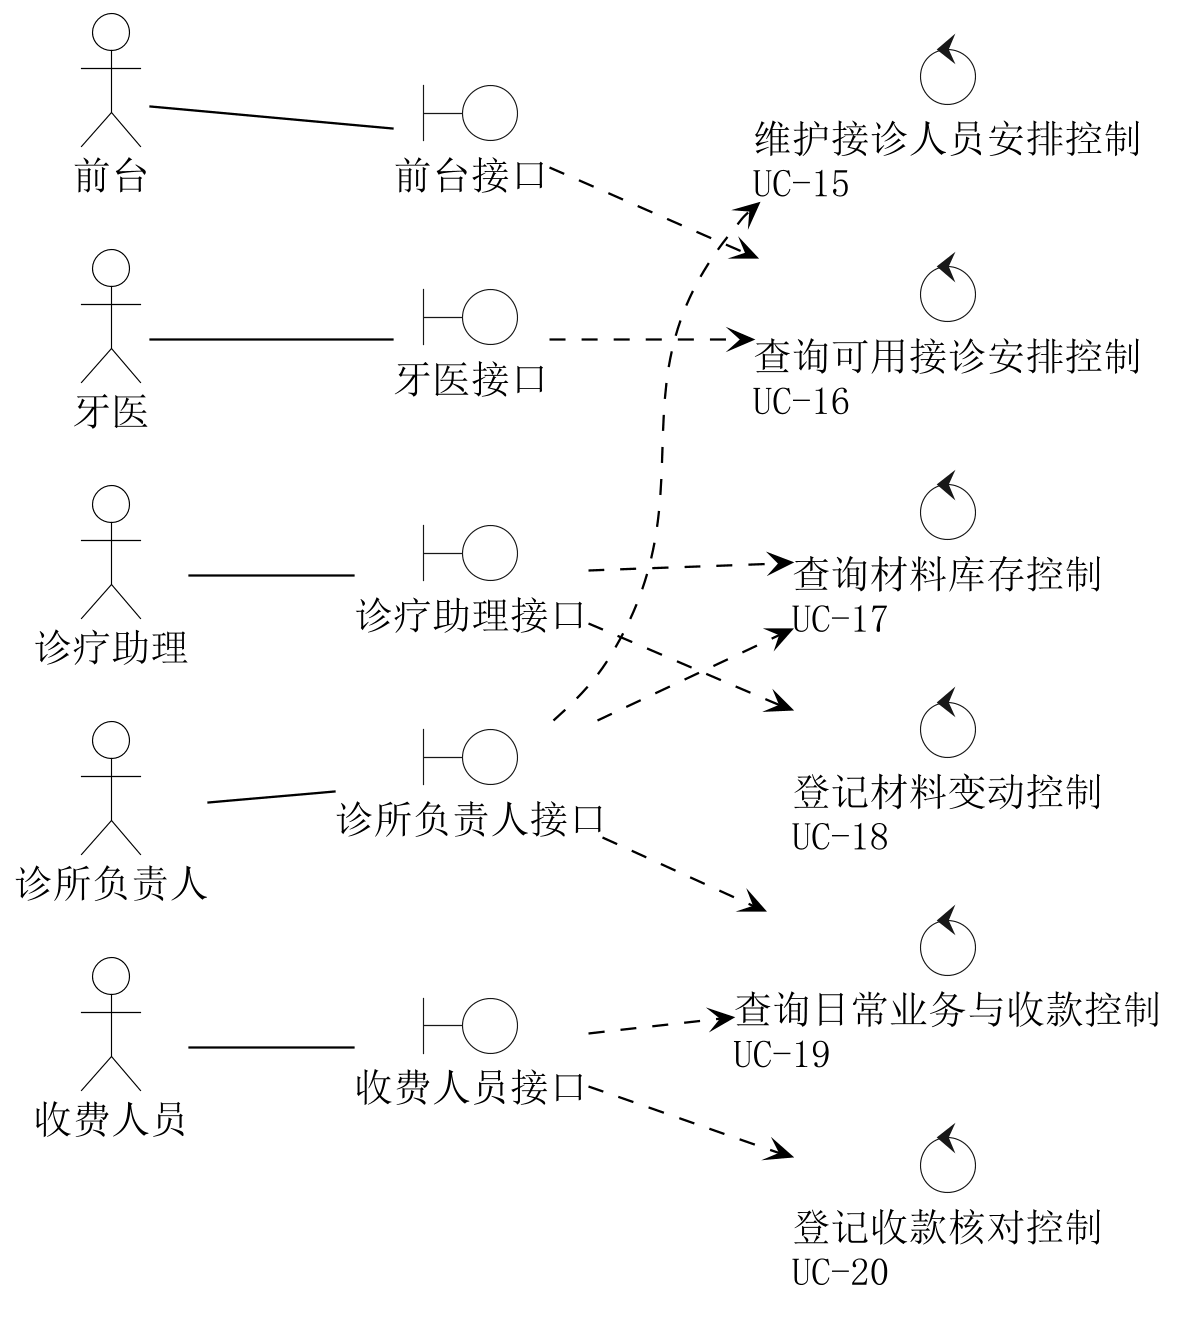
\includegraphics[width=\textwidth,height=19cm,keepaspectratio]{diagrams/10b-analysis-support-boundary-control.png}
\caption{分析类图：人员、材料与日常核对的边界类及控制类}
\label{fig:analysis-bc-support}
\end{figure}
\clearpage
\subsubsection{预约接待实体类}

预约接待涉及患者、职员、预约、预约变更和就诊；接诊时段提供确认依据，病历草稿由新就诊建立。诊疗收费中的“就诊”与本节为同一个分析类。

\begin{figure}[htbp]
\centering
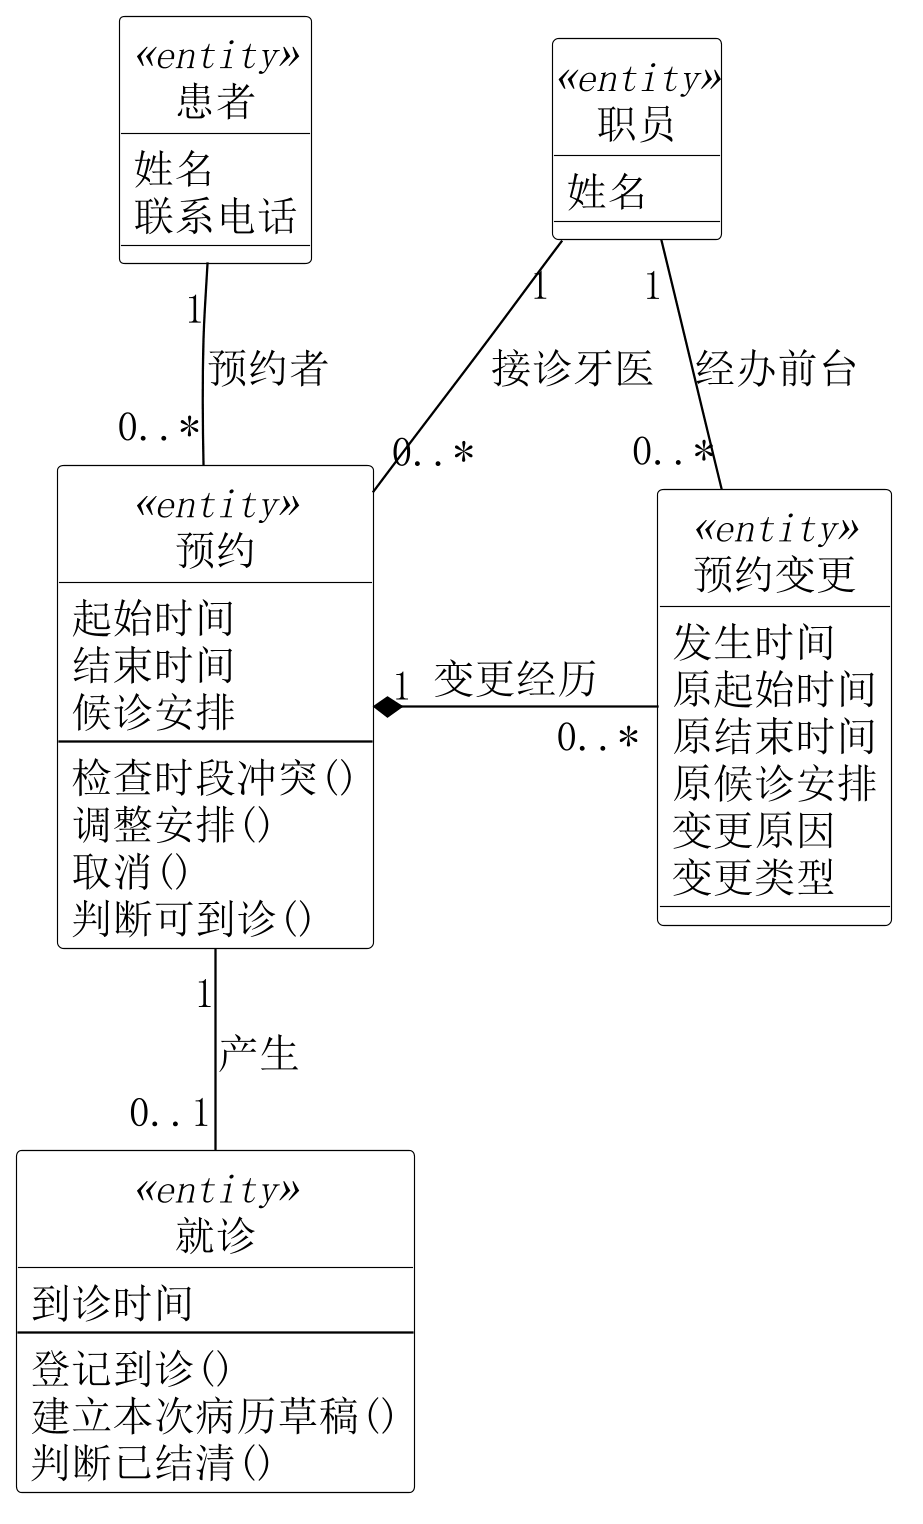
\includegraphics[width=\textwidth,height=14.0cm,keepaspectratio]{diagrams/11-analysis-reception-entities.png}
\caption{分析类图：预约接待实体}
\label{fig:analysis-reception}
\end{figure}

一位患者可有多次预约，每次预约对应一位接诊牙医。预约可积累多次变更，每次变更保存原安排、发生时间、原因及经办职员，以便追溯。每次就诊来自一条预约并建立一份病历草稿；一条预约至多产生一次就诊，重复登记返回原就诊及病历。

\clearpage
\subsubsection{诊疗收费实体类}

诊疗收费涉及就诊、诊疗确认、诊疗明细、收费项目、价目和现金收款。诊疗确认保存每次确认的项目版本，其组成明细表示实际完成的收费项目与数量。金额由明细计算并由诊疗确认汇总。

\begin{figure}[htbp]
\centering
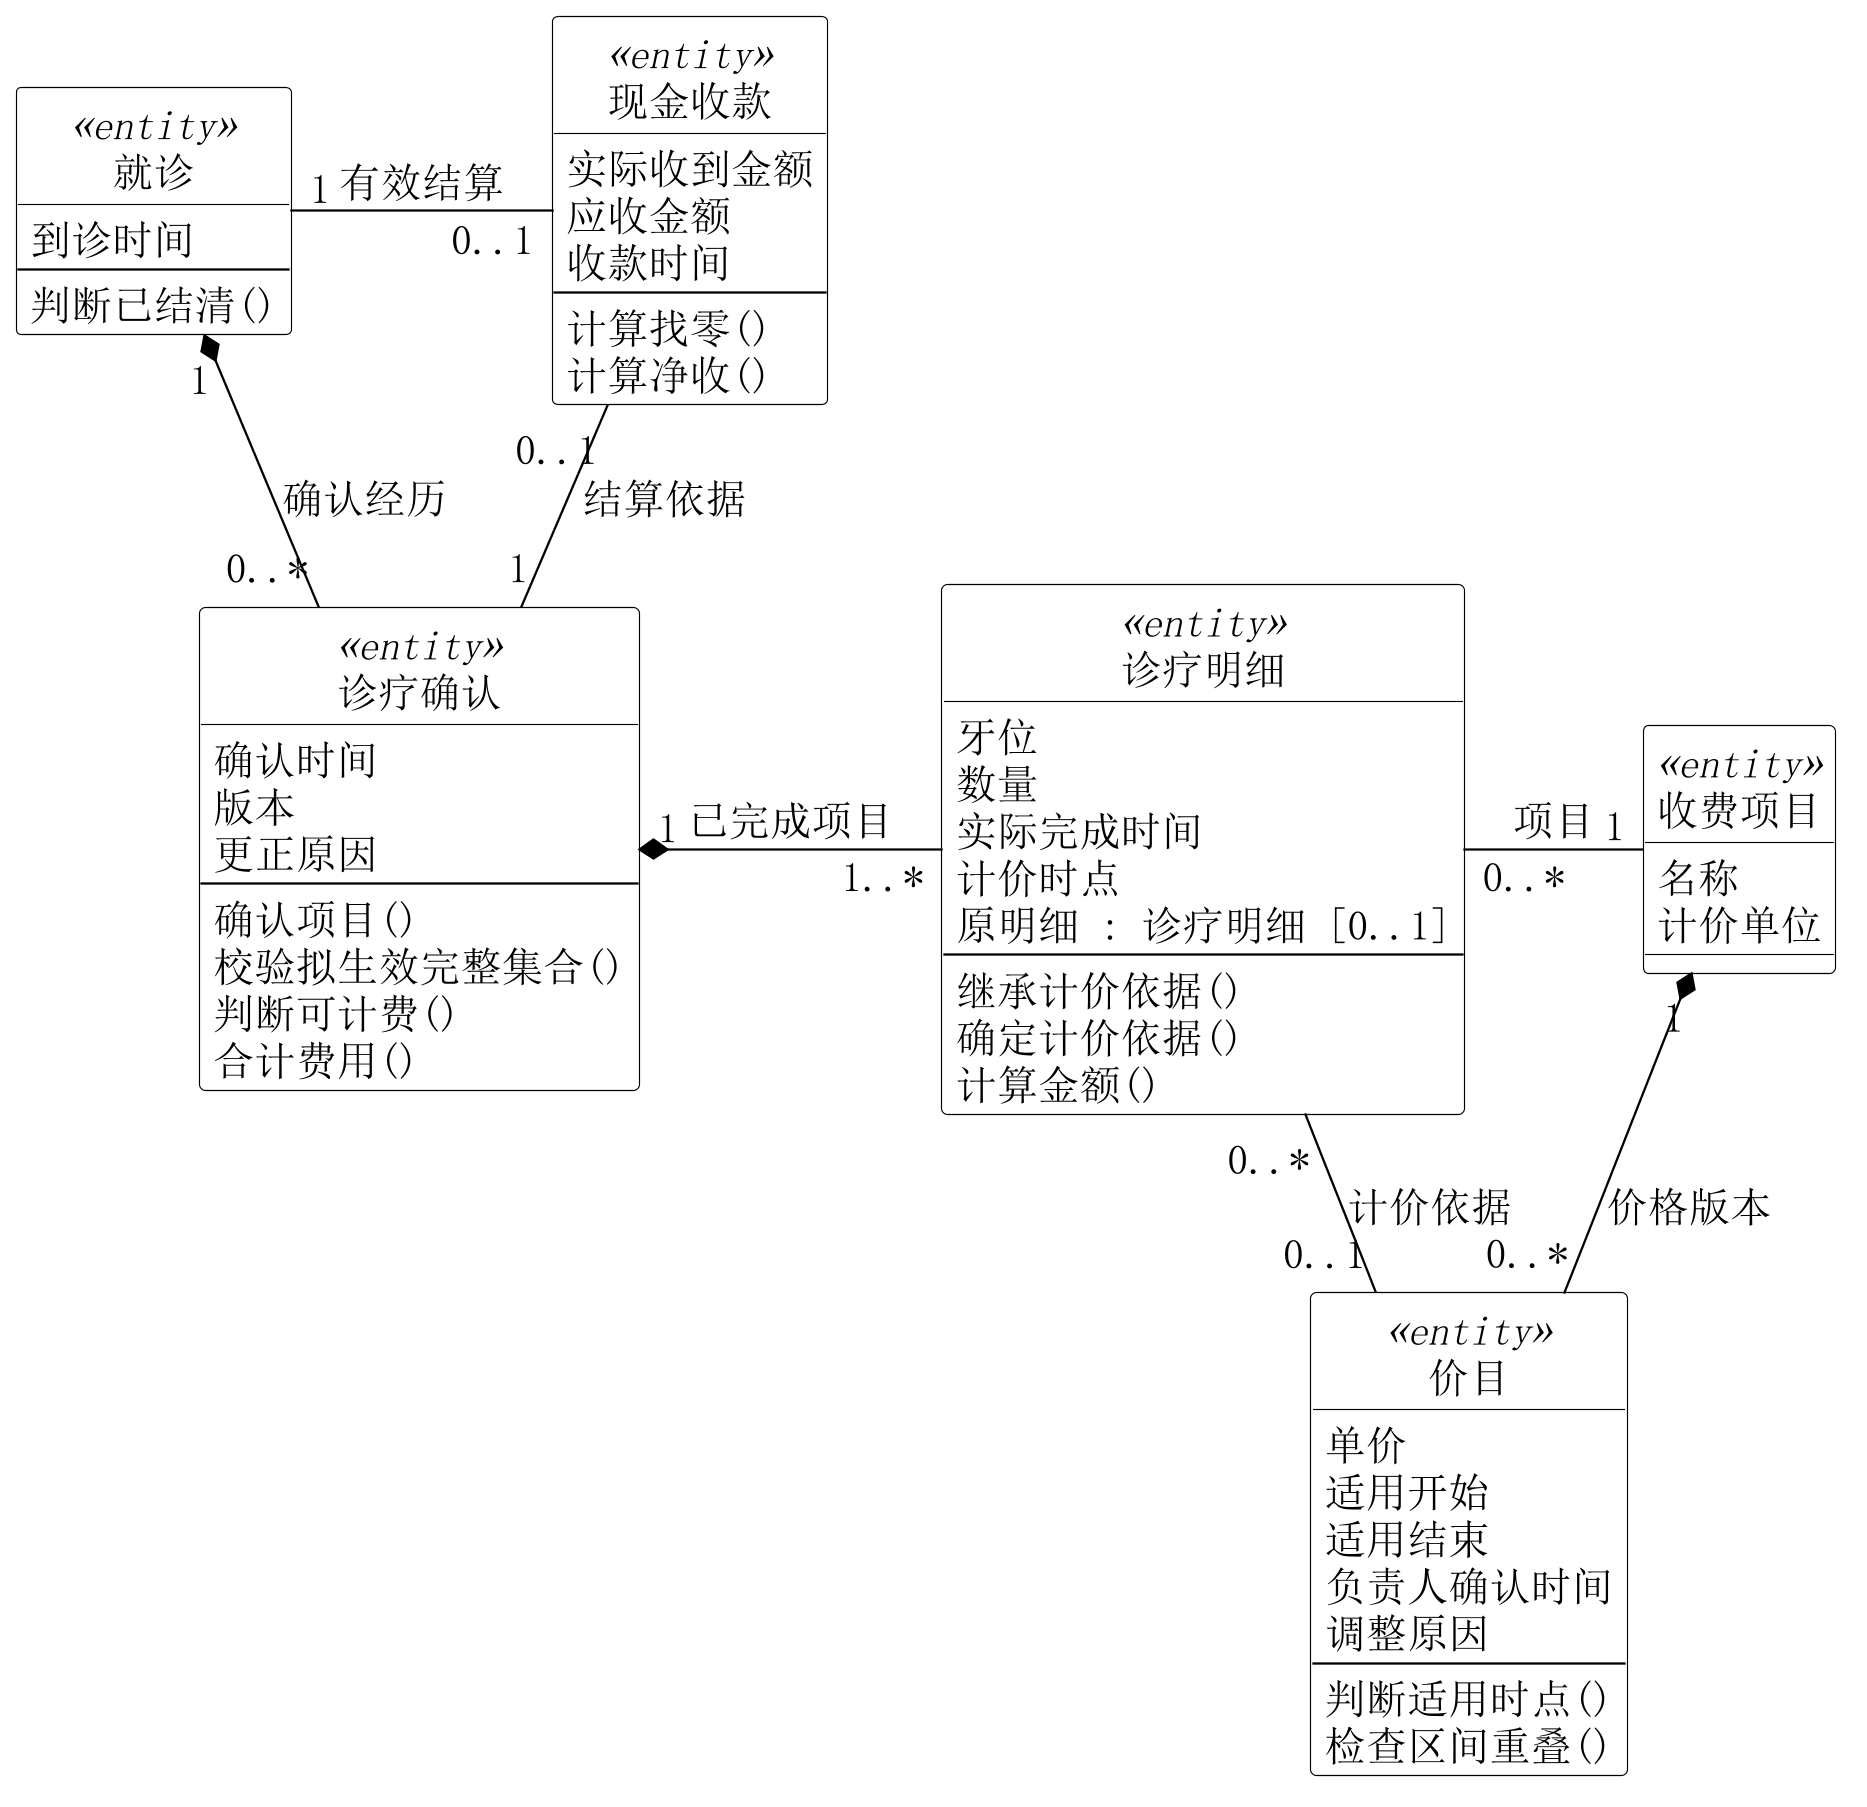
\includegraphics[width=\textwidth,height=11.3cm,keepaspectratio]{diagrams/12-analysis-billing-entities.png}
\caption{分析类图：诊疗收费实体}
\label{fig:analysis-billing}
\end{figure}

\noindent\textbf{关联约束}
\begin{enumerate}
\setlength{\itemsep}{0pt}
\item 就诊可有多个历史诊疗确认，只有当前确认版本可作为本次费用核对依据。更正产生新版本，历史版本及其明细保留。
\item 每个确认至少包含一条明细。同项目、同牙位且方案、计价与完成日期依据一致的明细合并；不同依据须先核实。
\item 同一项目同一时点至多有一个适用价目。既有同项目明细更正沿用原依据，新增或换项目按本次确认时点计价；实际完成时间供统计。
\item 明细与价目的0..1关系允许表达缺价；缺价时不能完成费用核对和收款，也不能把金额按零处理。补齐时仍按该明细保存的计价时点匹配适用价目。
\item 一次就诊至多一次有效现金收款，依据须属本次当前确认。收款与结清同时生效，结清后不得覆盖确认。
\end{enumerate}

收据来自原现金收款；找零为实收减应收，净收为应收。重新取得收据不产生新收款。

\clearpage
\clearpage
\subsubsection{患者与临床病历实体}
\begin{figure}[!htbp]
\centering
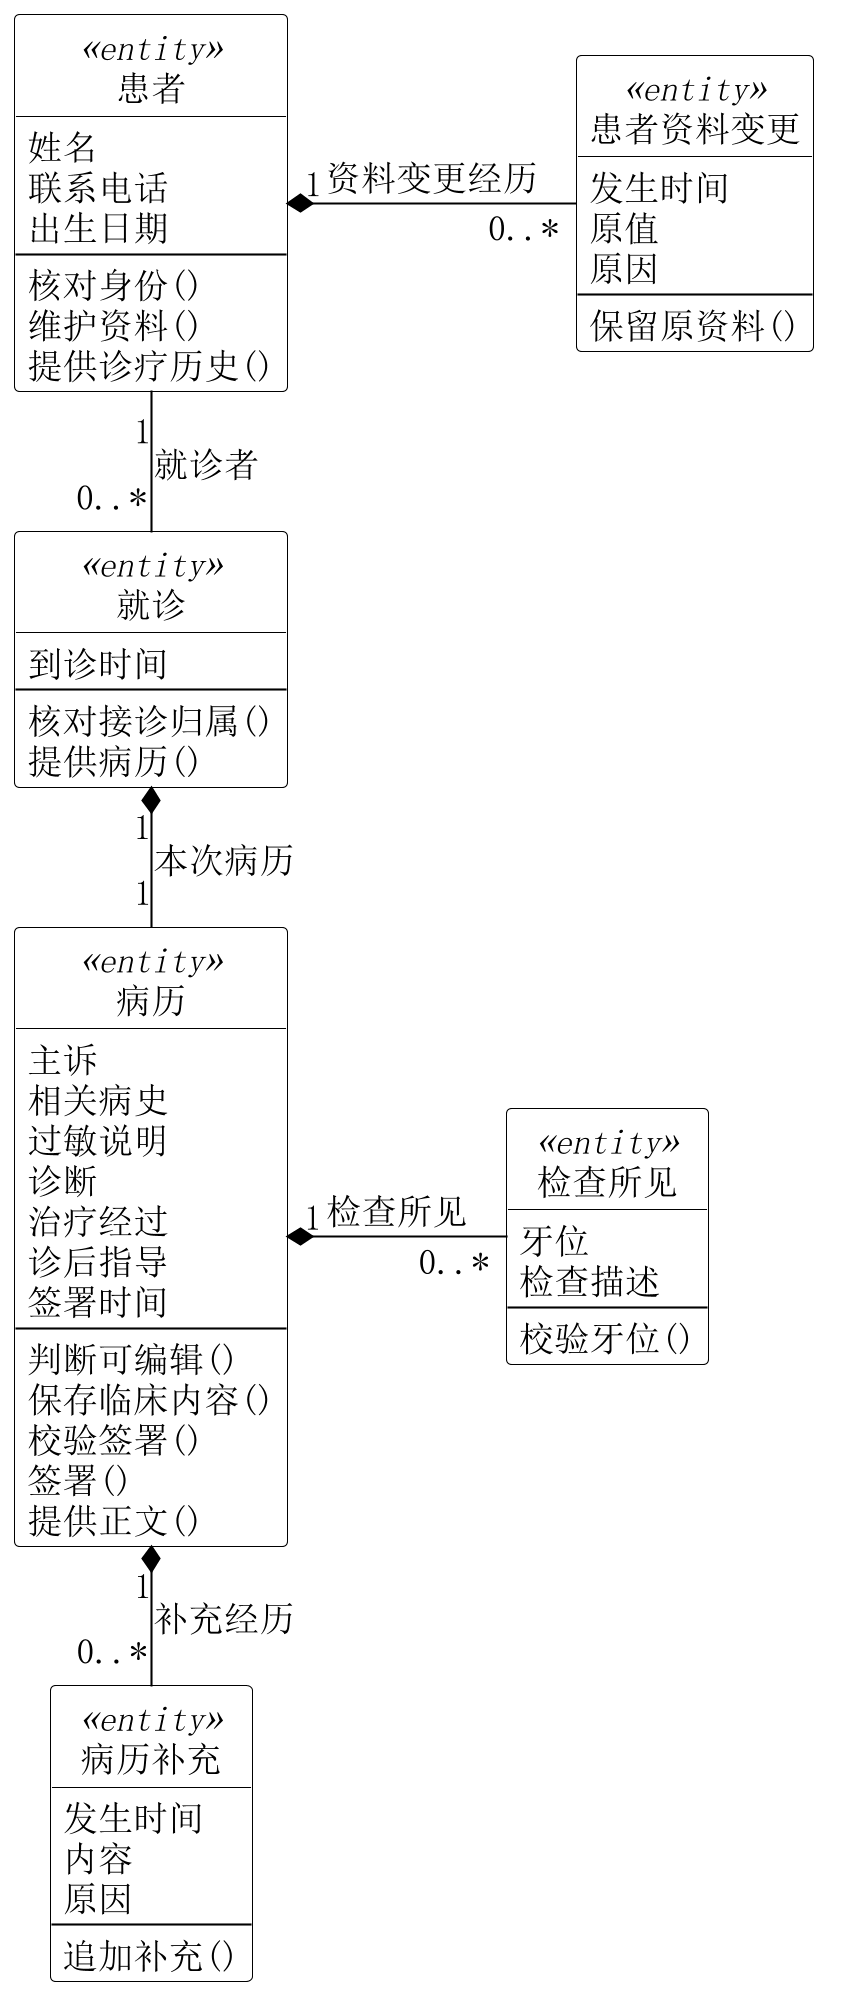
\includegraphics[width=\textwidth,height=17.5cm,keepaspectratio]{diagrams/12a-analysis-clinical-entities.png}
\caption{分析类图：患者与临床病历实体}
\label{fig:12a-analysis-clinical-entities}
\end{figure}

每次就诊关联一份病历；病历组织本次检查所见及补充。患者的资料变更保留原值，不能改变既有就诊归属。病历签署后原文保持不变，补充与原文分别可查。签署、补充及资料维护各关联一名实际经办职员。
\clearpage
\subsubsection{诊疗方案与实际项目实体}
\begin{figure}[!htbp]
\centering
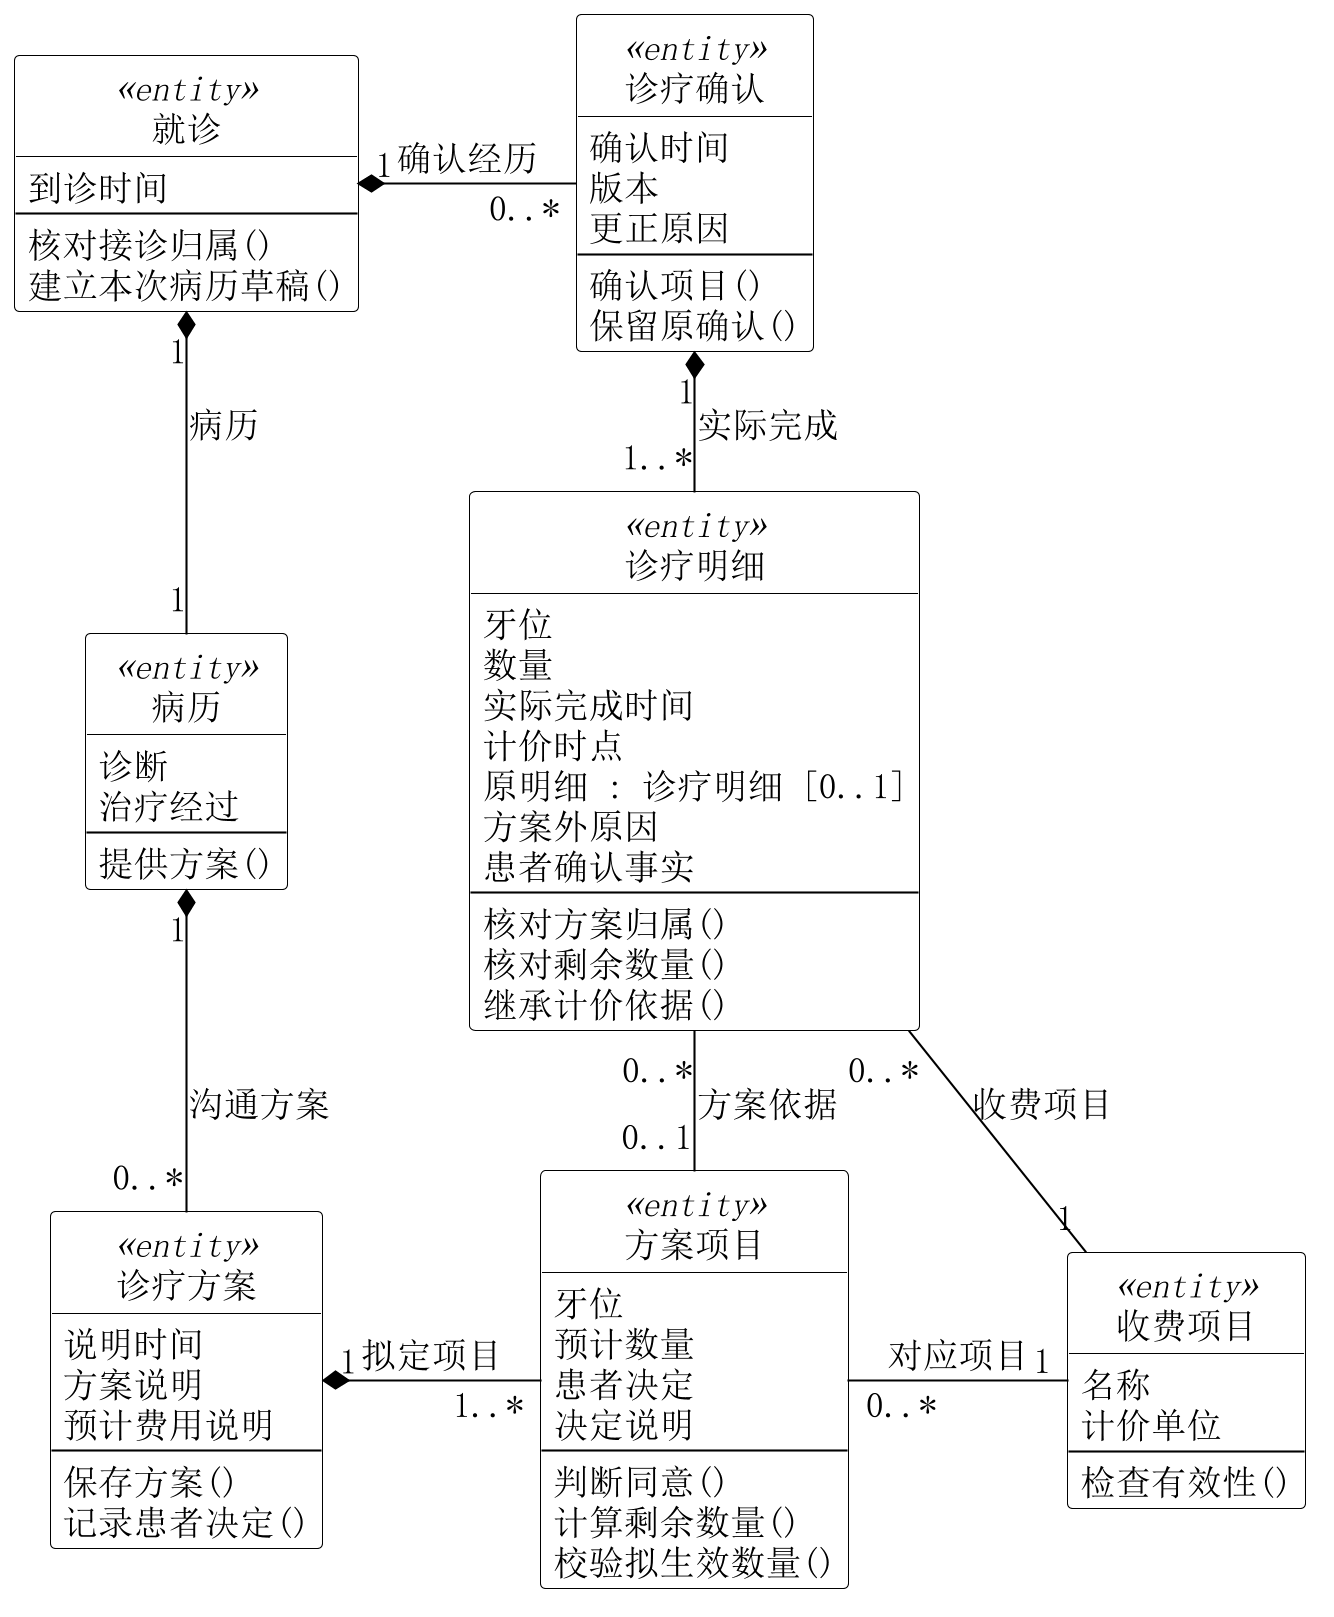
\includegraphics[width=\textwidth,height=17.5cm,keepaspectratio]{diagrams/12b-analysis-plan-entities.png}
\caption{分析类图：诊疗方案与实际项目实体}
\label{fig:12b-analysis-plan-entities}
\end{figure}

拟定方案与实际完成项目分开。实际明细可关联本次就诊的一个方案项目；关联时须核对牙位、项目、患者决定及剩余数量。没有方案依据的实际项目须保留原因及患者确认事实。预计数量与实际数量的比较只取拟生效完整明细集合；更正替换当前确认后重算，历史确认不重复计入已完成数量。同项目不同牙位分别保留，不能为了合计费用抹去牙位。
\clearpage
\subsubsection{复诊随访实体}
\begin{figure}[!htbp]
\centering
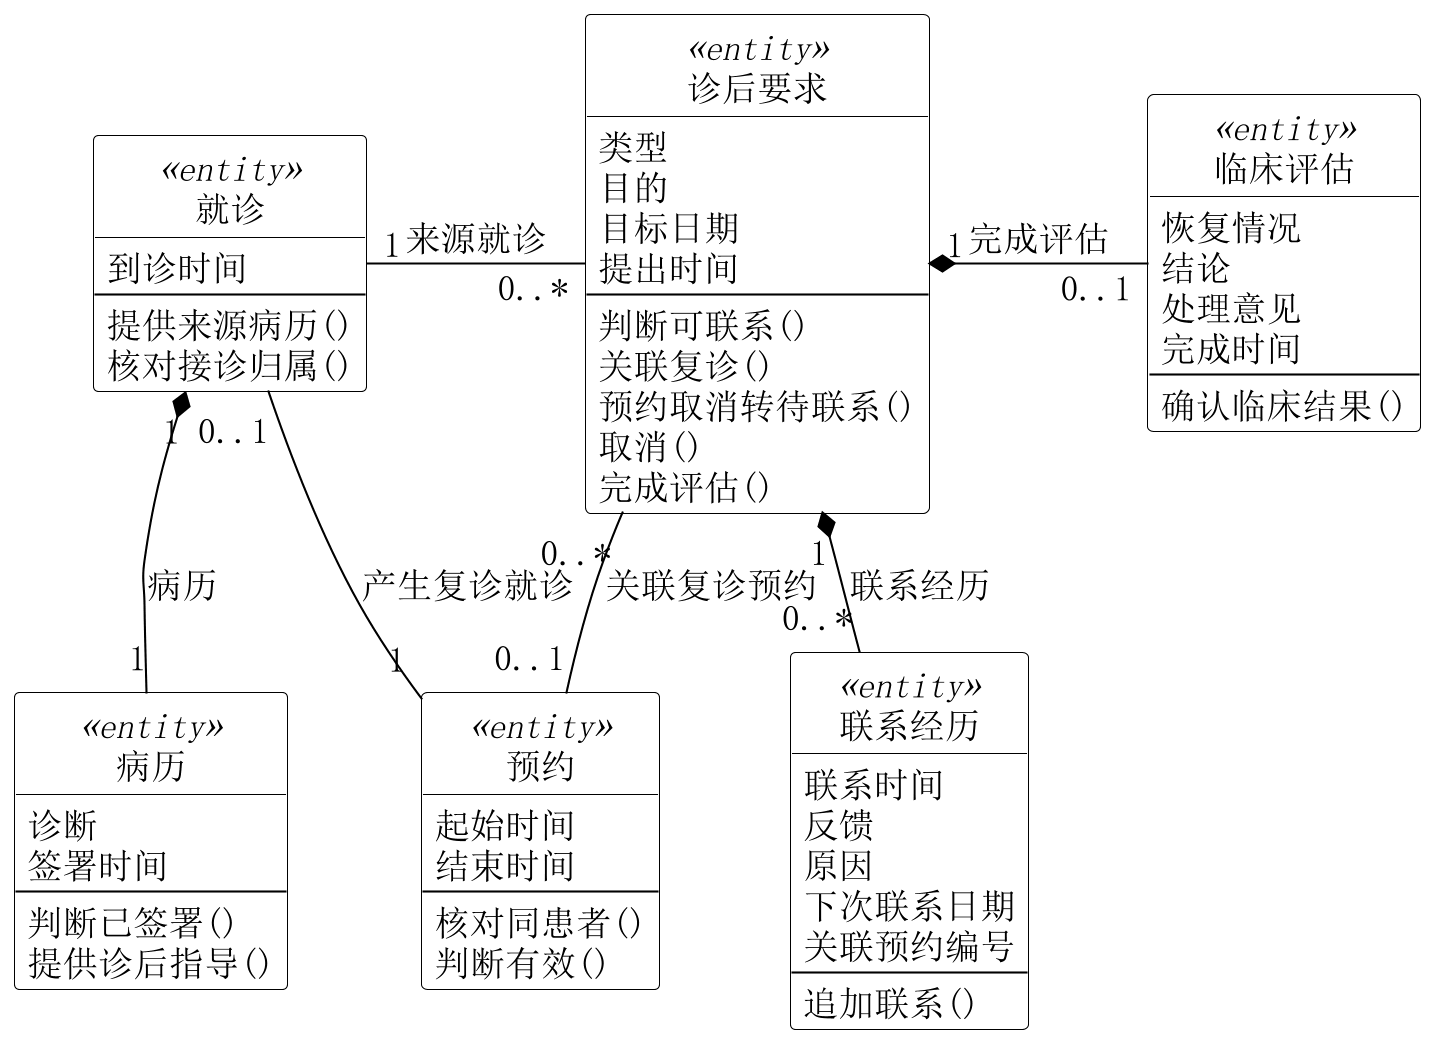
\includegraphics[width=\textwidth,height=17.5cm,keepaspectratio]{diagrams/12c-analysis-followup-entities.png}
\caption{分析类图：复诊随访实体}
\label{fig:12c-analysis-followup-entities}
\end{figure}

诊后要求由一个已签署来源就诊提出，可积累多次联系；需要复诊时关联同患者的有效预约。复诊预约产生的就诊与来源就诊是同一分析类的不同对象。前台联系不能替代临床评估；每个要求至多有一个完成评估。提出牙医、经办前台及评估牙医分别关联职员。
\clearpage
\subsubsection{接诊人员安排实体}
\begin{figure}[!htbp]
\centering
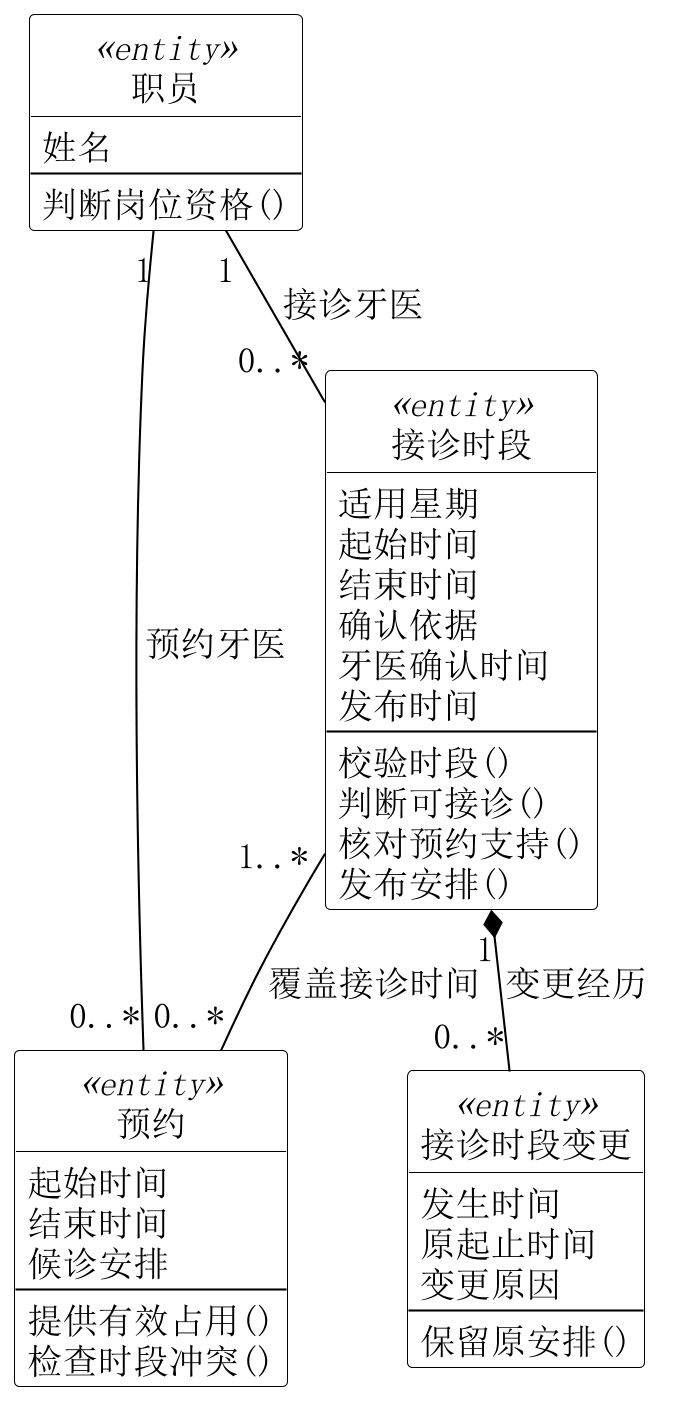
\includegraphics[width=\textwidth,height=17.5cm,keepaspectratio]{diagrams/12d-analysis-staffing-entities.png}
\caption{分析类图：接诊人员安排实体}
\label{fig:12d-analysis-staffing-entities}
\end{figure}

有效预约的全部时间须被其接诊牙医的有效接诊时段覆盖；同一时段可以支撑多次不重叠预约。接诊时段按每周星期及起止时间表达，判定时转换到预约的同一当地日期和时间。接诊时段变更保留原起止时间及原因，发布人及确认牙医关联职员；尚未协调的已有预约不能因变更时段失去接诊支持。
\clearpage
\subsubsection{诊疗材料实体}
\begin{figure}[!htbp]
\centering
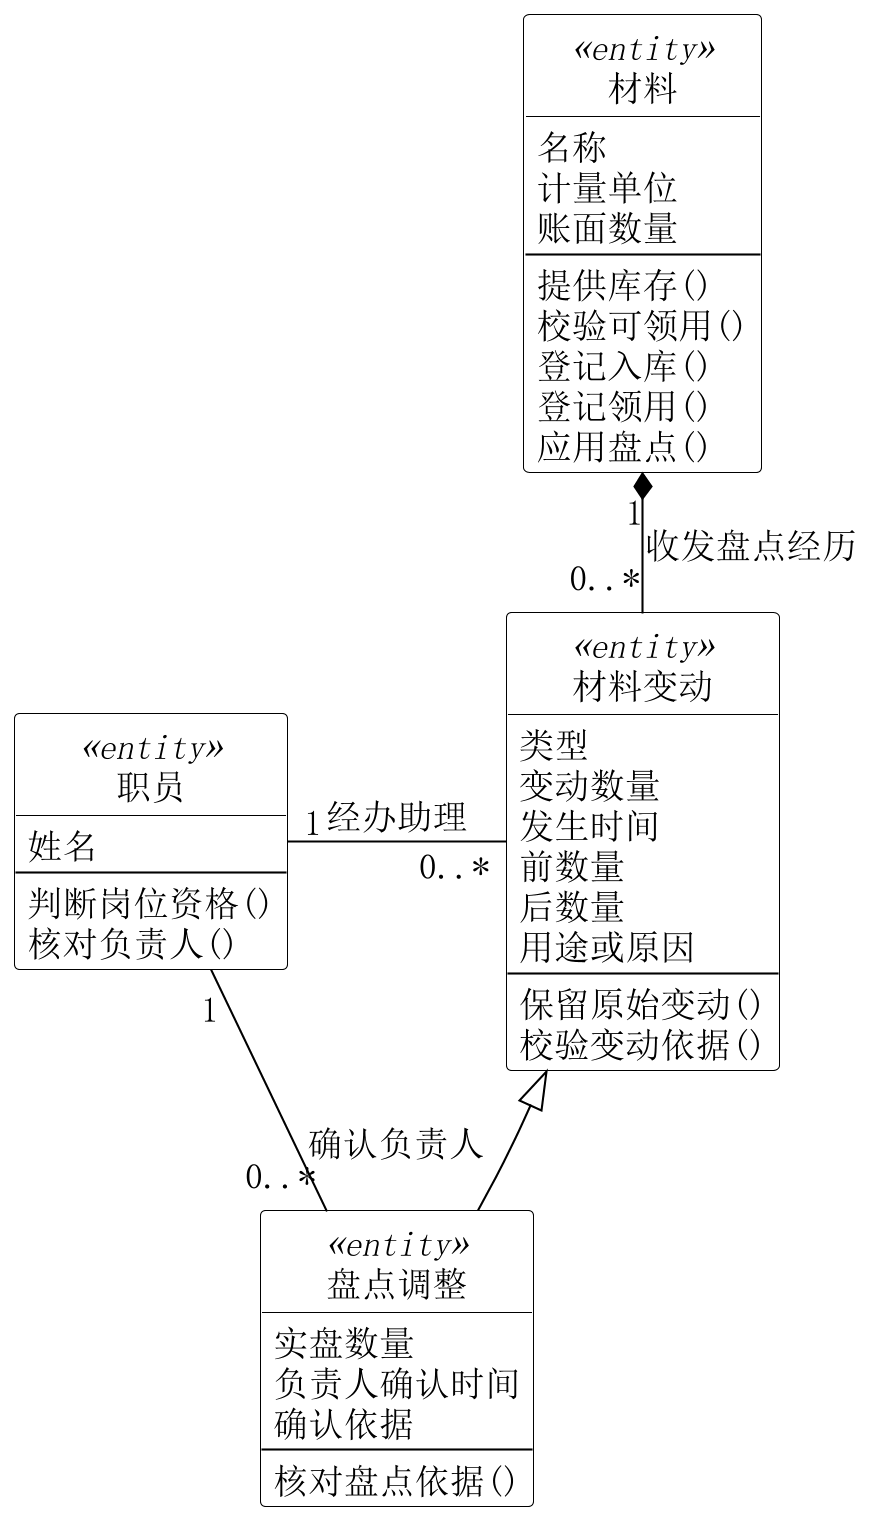
\includegraphics[width=\textwidth,height=17.5cm,keepaspectratio]{diagrams/12e-analysis-materials-entities.png}
\caption{分析类图：诊疗材料实体}
\label{fig:12e-analysis-materials-entities}
\end{figure}

每次变动对应一种材料及一名助理；盘点调整是材料变动的一种，保留实盘数量及确认依据，并关联一名有效确认负责人。材料的账面数量由入库、领用及已确认盘点得到。前后数量及用途保留为原始经历，领用不得使库存为负。
\clearpage
\subsubsection{日常收款核对实体}
\begin{figure}[!htbp]
\centering
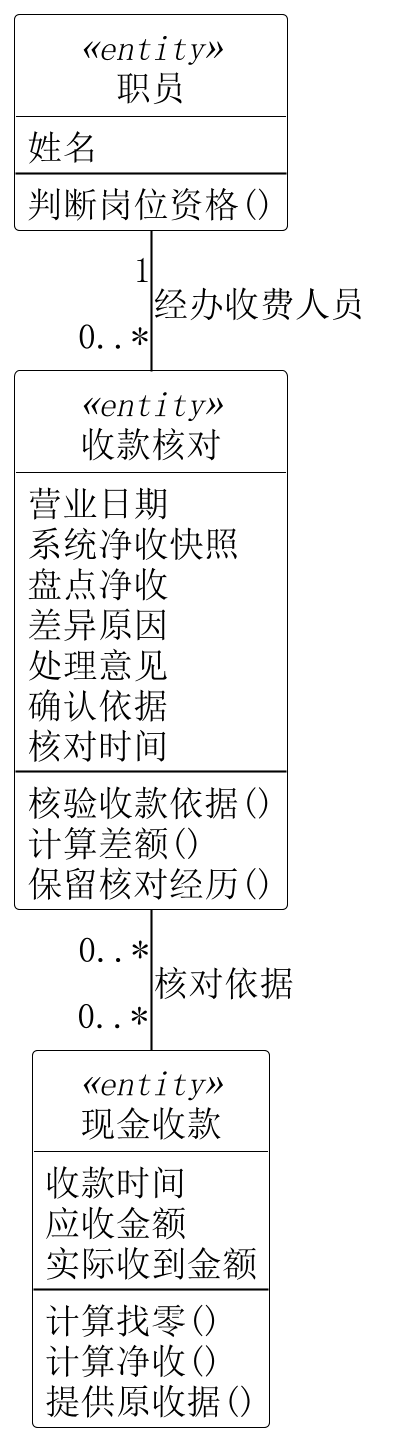
\includegraphics[width=\textwidth,height=17.5cm,keepaspectratio]{diagrams/12f-analysis-reconciliation-entities.png}
\caption{分析类图：日常收款核对实体}
\label{fig:12f-analysis-reconciliation-entities}
\end{figure}

收款核对保留当日引用的有效现金收款及其汇总快照。系统净收与盘点净收的差额由核对计算；差异说明及负责人处理依据不反向修改任何原收据。不同次核对可引用同一组原收款，原核对经历保留。经营汇总由控制类协调就诊、实际项目及现金收款查询，不另造保存重复业务事实的报表实体。
\clearpage
\subsubsection{用例与分析类的责任对应}

表\ref{tab:analysis-responsibilities}明确各控制类的主要协作实体。边界类负责输入输出，控制类组织步骤，实体类完成业务判断并维护自身的一致性。

\begin{table}[htbp]
\centering
\caption{用例与分析类的责任对应（UC-01至UC-07）}
\label{tab:analysis-responsibilities}
\small
\renewcommand{\arraystretch}{1.25}
\begin{tabularx}{\textwidth}{@{}p{1.2cm}>{\raggedright\arraybackslash}p{4cm}L@{}}
\toprule
用例 & 边界类／控制类 & 主要实体与责任 \\
\midrule
UC-01 & 前台接口／维护预约及接诊安排控制 & 患者编号定位身份；接诊时段提供牙医确认依据，职员核对资格；预约检查冲突及变更，取消复诊预约时协调未终结诊后要求回待联系。 \\
UC-02 & 前台接口／查询预约及接诊安排控制 & 患者、预约、职员共同提供匹配的预约及接诊安排；查询保持业务内容不变。 \\
UC-03 & 前台接口／登记到诊控制 & 预约判断可到诊；就诊建立并关联病历草稿；控制类协调三者同时生效，重复请求返回原结果。 \\
UC-04 & 牙医接口／确认诊疗项目控制 & 就诊限定范围；明细保存牙位及实际完成时间，方案项目判断同意及拟生效数量；明细继承或匹配计价依据，诊疗确认组织有效版本。 \\
UC-05 & 收费人员接口／维护收费价目控制 & 收费项目组织价格版本，价目检查适用区间；职员关联确认负责人和维护人员。 \\
UC-06 & 收费人员接口／查询待结算费用控制 & 就诊与现金收款确定是否已结清；诊疗确认判断可计费，明细依价目计算金额，诊疗确认汇总费用。 \\
UC-07 & 收费人员接口／登记现金收款控制 & 就诊与诊疗确认保证结算依据一致；现金收款保存款项并计算找零；职员确定操作者，控制类协调收款与结清同时生效。 \\
\bottomrule
\end{tabularx}
\end{table}

\clearpage
\begin{table}[!htbp]
\centering
\caption{用例与分析类的责任对应（UC-08至UC-14）}
\label{tab:new-responsibility-0}
\small
\renewcommand{\arraystretch}{1.18}
\begin{tabularx}{\textwidth}{@{}>{\raggedright\arraybackslash}p{1.2cm}>{\raggedright\arraybackslash}p{6.0cm}L@{}}
\toprule
用例 & 边界类／控制类 & 协作实体 \\
\midrule
UC-08 & 前台接口／维护患者资料控制 & 患者、患者资料变更、职员 \\
UC-09 & 牙医接口／查询患者诊疗资料控制 & 就诊、患者、病历、病历补充 \\
UC-10 & 牙医接口／记录检查诊断及方案控制 & 就诊、病历、检查所见、诊疗方案、方案项目 \\
UC-11 & 牙医接口／签署及补充病历控制 & 就诊、病历、病历补充、诊疗确认 \\
UC-12 & 牙医接口／提出复诊随访要求控制 & 就诊、病历、诊后要求、职员 \\
UC-13 & 前台接口／办理复诊随访联系控制 & 诊后要求、联系经历、预约、职员 \\
UC-14 & 牙医接口／记录复诊随访评估控制 & 诊后要求、临床评估、预约、就诊、病历 \\
\bottomrule
\end{tabularx}
\end{table}
\clearpage
\begin{table}[!htbp]
\centering
\caption{用例与分析类的责任对应（UC-15至UC-20）}
\label{tab:new-responsibility-1}
\small
\renewcommand{\arraystretch}{1.18}
\begin{tabularx}{\textwidth}{@{}>{\raggedright\arraybackslash}p{1.2cm}>{\raggedright\arraybackslash}p{6.0cm}L@{}}
\toprule
用例 & 边界类／控制类 & 协作实体 \\
\midrule
UC-15 & 诊所负责人接口／维护接诊人员安排控制 & 职员、接诊时段、接诊时段变更、预约 \\
UC-16 & 前台、牙医接口／查询可用接诊安排控制 & 职员、接诊时段、预约 \\
UC-17 & 诊疗助理、诊所负责人接口／查询材料库存控制 & 材料、材料变动、职员 \\
UC-18 & 诊疗助理接口／登记材料变动控制 & 材料、材料变动、盘点调整、职员 \\
UC-19 & 收费人员、诊所负责人接口／查询日常业务与收款控制 & 就诊、诊疗确认、诊疗明细、现金收款 \\
UC-20 & 收费人员接口／登记收款核对控制 & 现金收款、收款核对、职员 \\
\bottomrule
\end{tabularx}
\end{table}

临床评估、联系经历、患者资料变更、材料变动及收款核对保留各自的发生时间、经办职员和业务依据；同名实体在不同视图中为同一个类，不因岗位或图的划分复制患者、就诊或职员。
\clearpage
职员通过关联中的角色承担业务责任，一名职员可以兼任不同岗位。各实体视图中未展开的职员关联补充如下。

{\small
\renewcommand{\arraystretch}{1.15}
\noindent\begin{tabularx}{\textwidth}{@{}>{\raggedright\arraybackslash}p{2.5cm}L@{}}
\toprule
关联对象 & 职员角色及数量 \\
\midrule
预约 & 每次预约有1名登记前台及1名接诊牙医；安排确认牙医为所用接诊时段的确认人，可与接诊牙医相同。 \\
预约变更 & 每次变更有1名经办前台；涉及换医时保留1名原接诊牙医。 \\
就诊 & 每次到诊登记有1名经办前台，接诊牙医由预约安排确定。 \\
诊疗确认 & 每次确认有1名确认牙医，须为该次接诊牙医。 \\
价目 & 每个价格版本有1名确认负责人及1名维护收费人员。 \\
现金收款 & 每次收款登记有1名经办收费人员。 \\
\bottomrule
\end{tabularx}\par
}

预约冲突由患者或牙医在相同时段的有效预约关系判断；重复到诊由预约与就诊的一对至多一关系约束；重复收款由就诊与现金收款的一对至多一关系约束。并发操作仍须遵守这些业务约束。

预约编号、就诊编号及收款编号按用例规约用于业务定位与凭据展示。预约与就诊的生命周期见第\ref{sec:analysis-state}节。


\clearpage
\subsection{分析序列图}
\label{sec:analysis-sequence}
\subsubsection{UC-01：维护预约及接诊安排}
\medskip

图\ref{fig:seq-01}将新增预约分配给前台接口、维护预约及接诊安排控制、患者、职员、接诊时段和预约。前台接口检查输入格式；职员判断人员资格；预约承担患者与牙医的时段冲突判断，并在保存时再次检查。

\begin{figure}[!htbp]
\centering
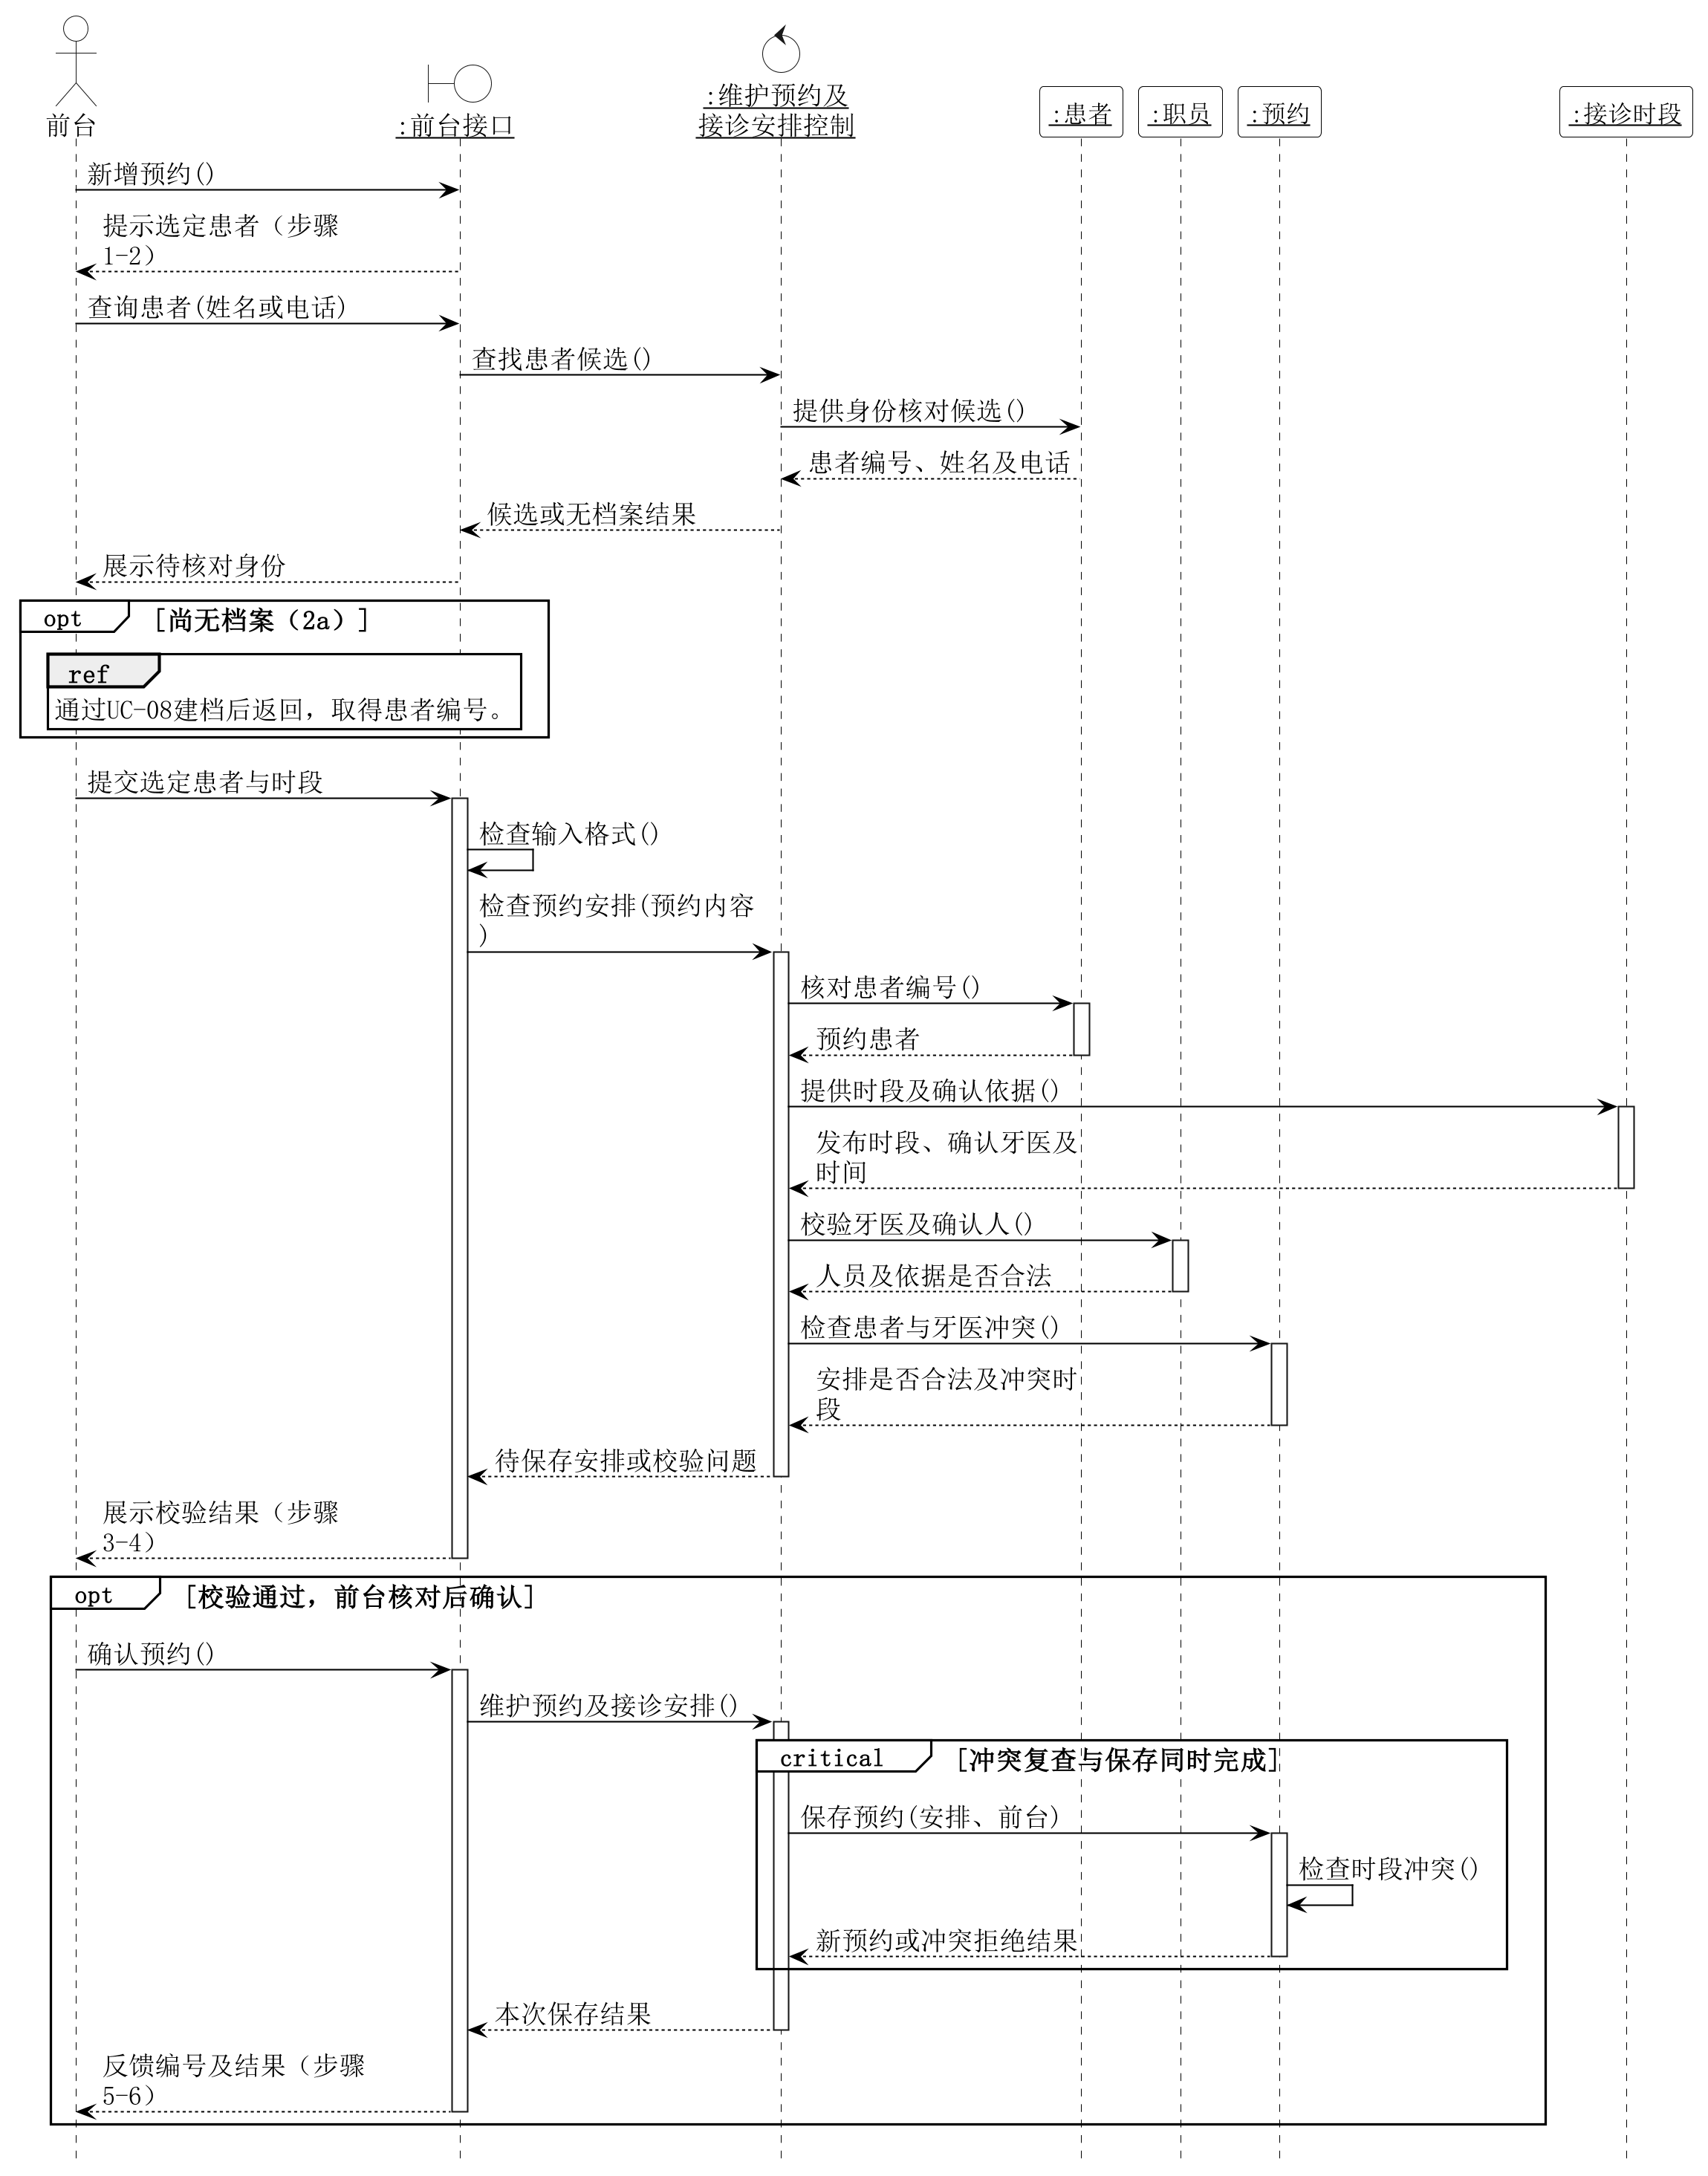
\includegraphics[width=\textwidth,height=19cm,keepaspectratio]{diagrams/13-01-analysis-sequence.png}
\caption{UC-01 基本路径分析序列图（扩展见图\ref{fig:seq-01-ext}）}
\label{fig:seq-01}
\end{figure}
\clearpage
\noindent\textbf{UC-01 分析序列图：修改与取消预约}
\medskip

图\ref{fig:seq-01-ext}对应扩展1a、1b，并体现4a与6a的拒绝条件。修改及取消由预约承担，预约变更保留原安排、原因及经办职员。返回新增流程时使用图\ref{fig:seq-01}；修改涉及的患者、牙医资格和时段规则沿用其校验责任。

\begin{figure}[!htbp]
\centering
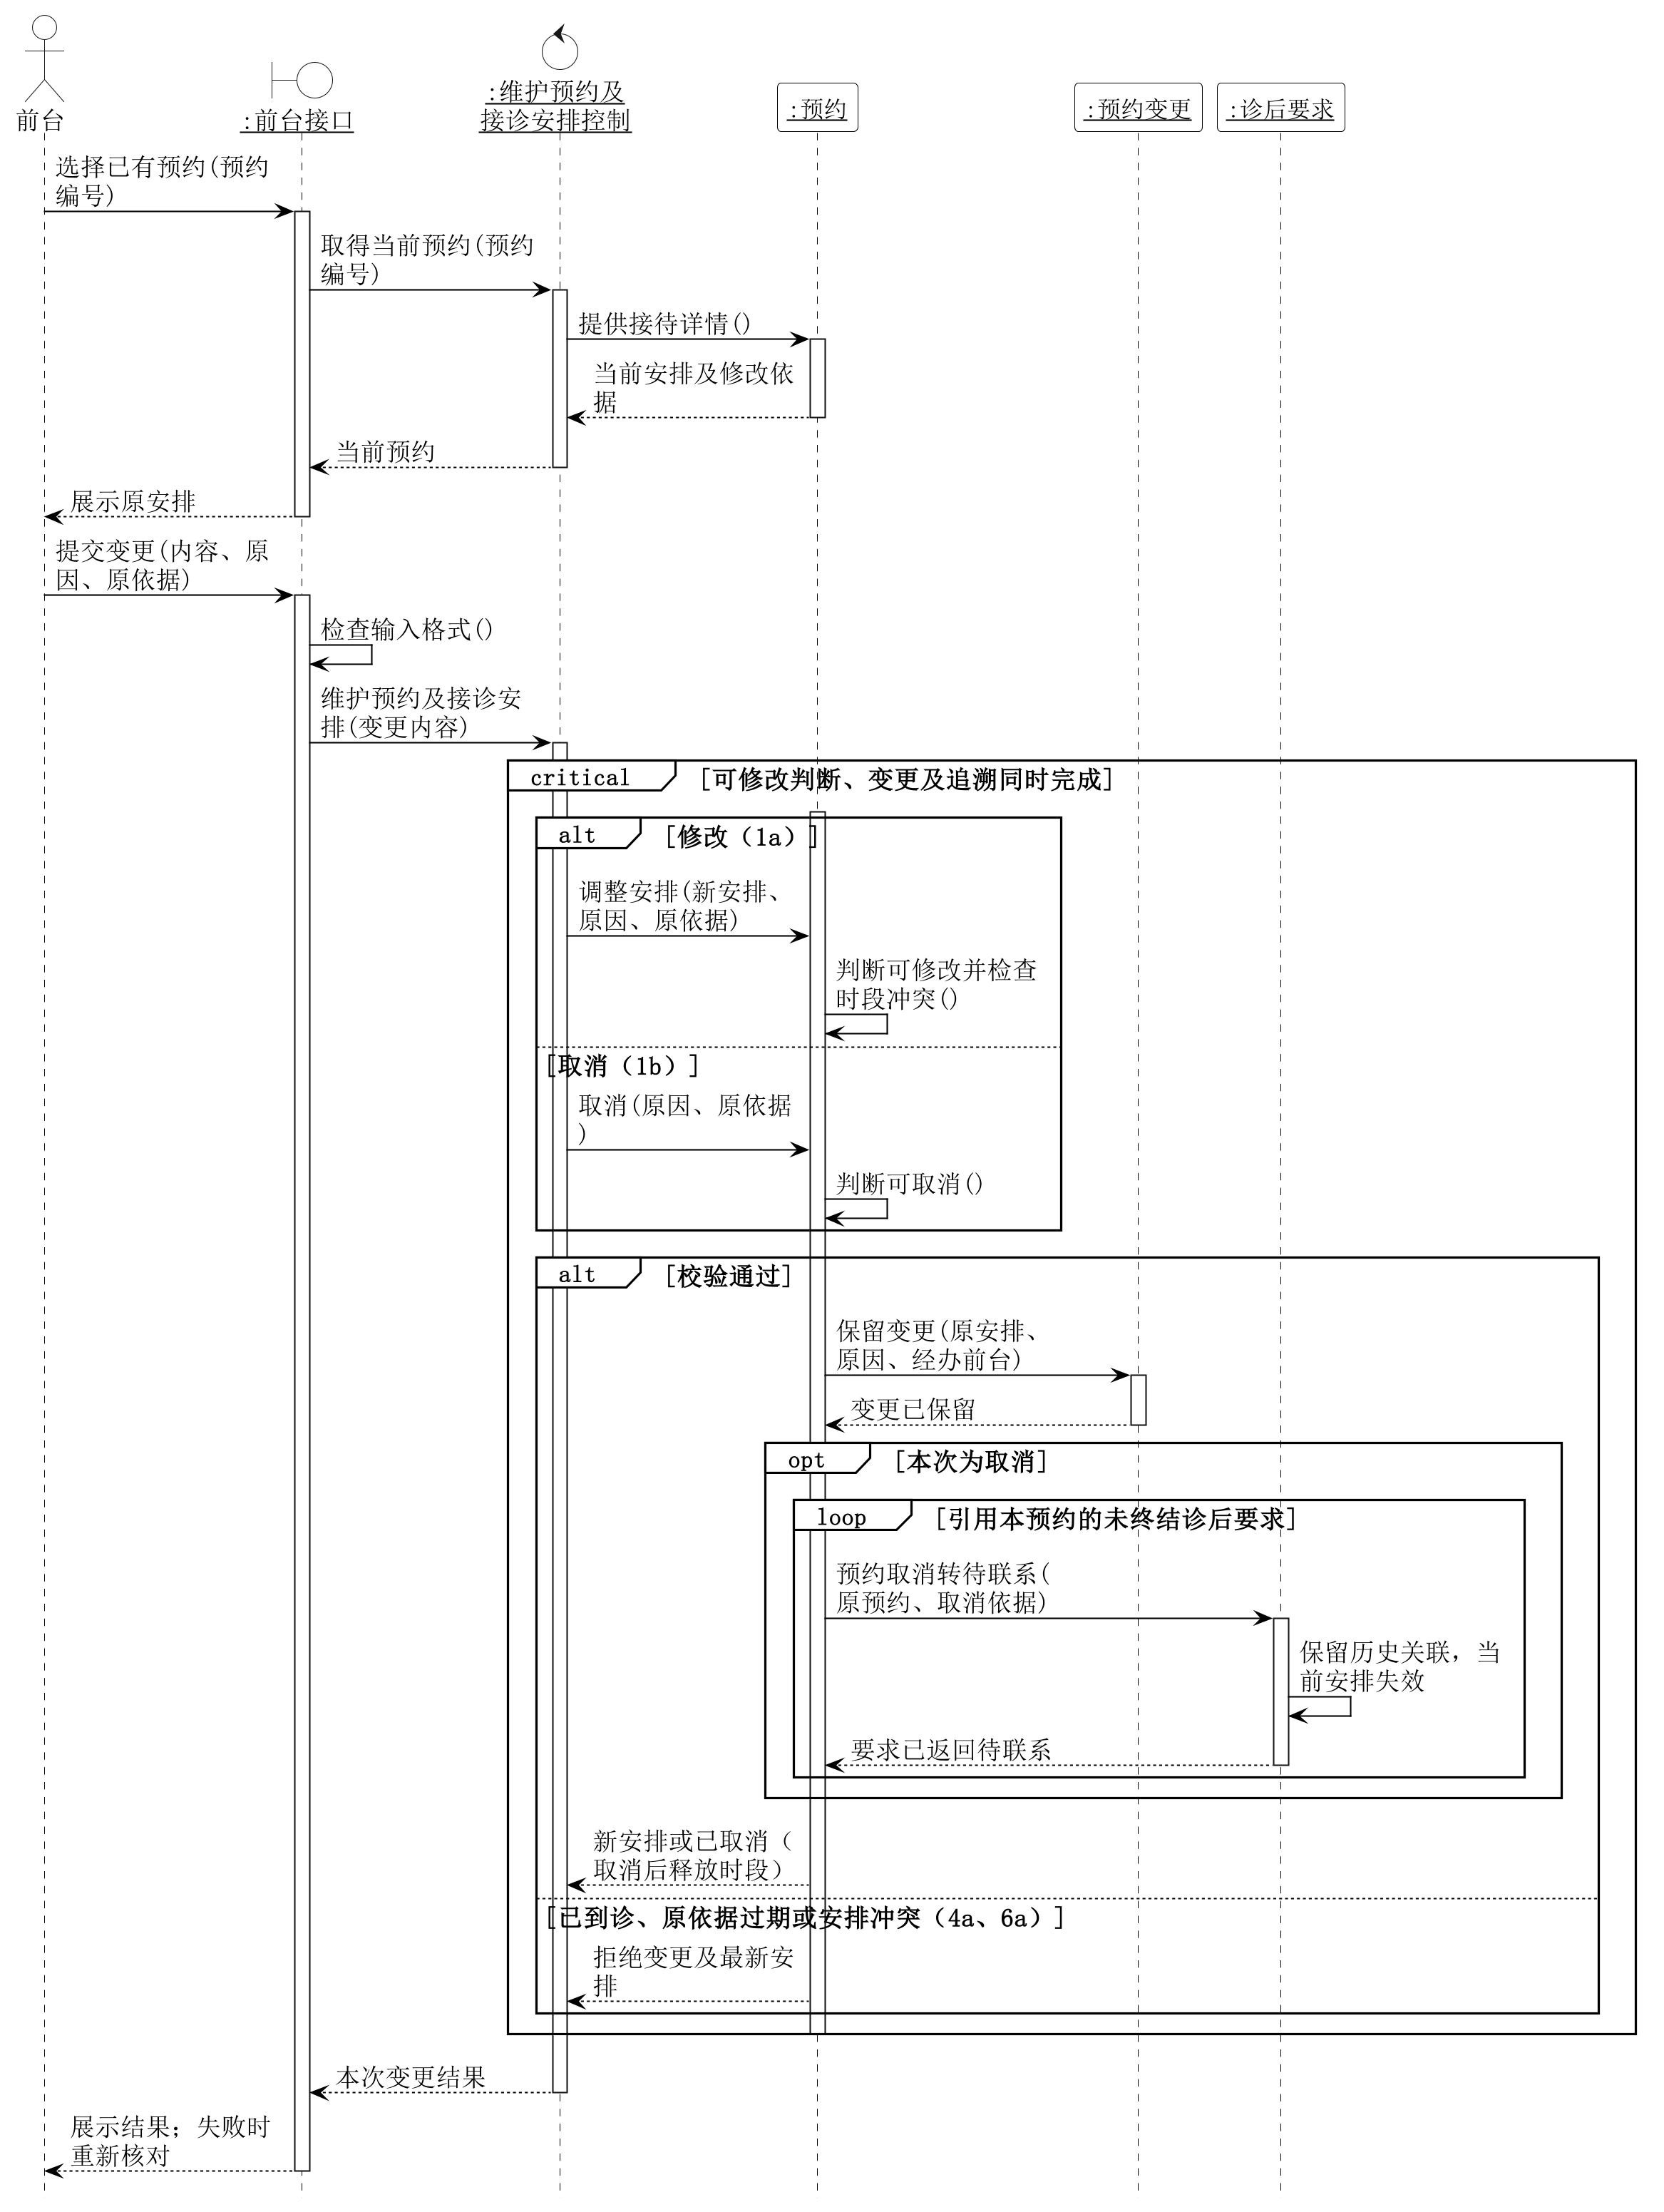
\includegraphics[width=\textwidth,height=20.4cm,keepaspectratio]{diagrams/13-01a-analysis-sequence.png}
\caption{UC-01 修改与取消预约分析序列图}
\label{fig:seq-01-ext}
\end{figure}

\clearpage
\subsubsection{UC-02：查询预约及接诊安排}
\medskip

图\ref{fig:seq-02}对应预约查询的基本路径。患者负责匹配身份条件，预约组织所选日期的安排，职员提供接诊信息。前台从可区分的候选记录中选定本次预约；读取详情时取得当前内容。

\begin{figure}[!htbp]
\centering
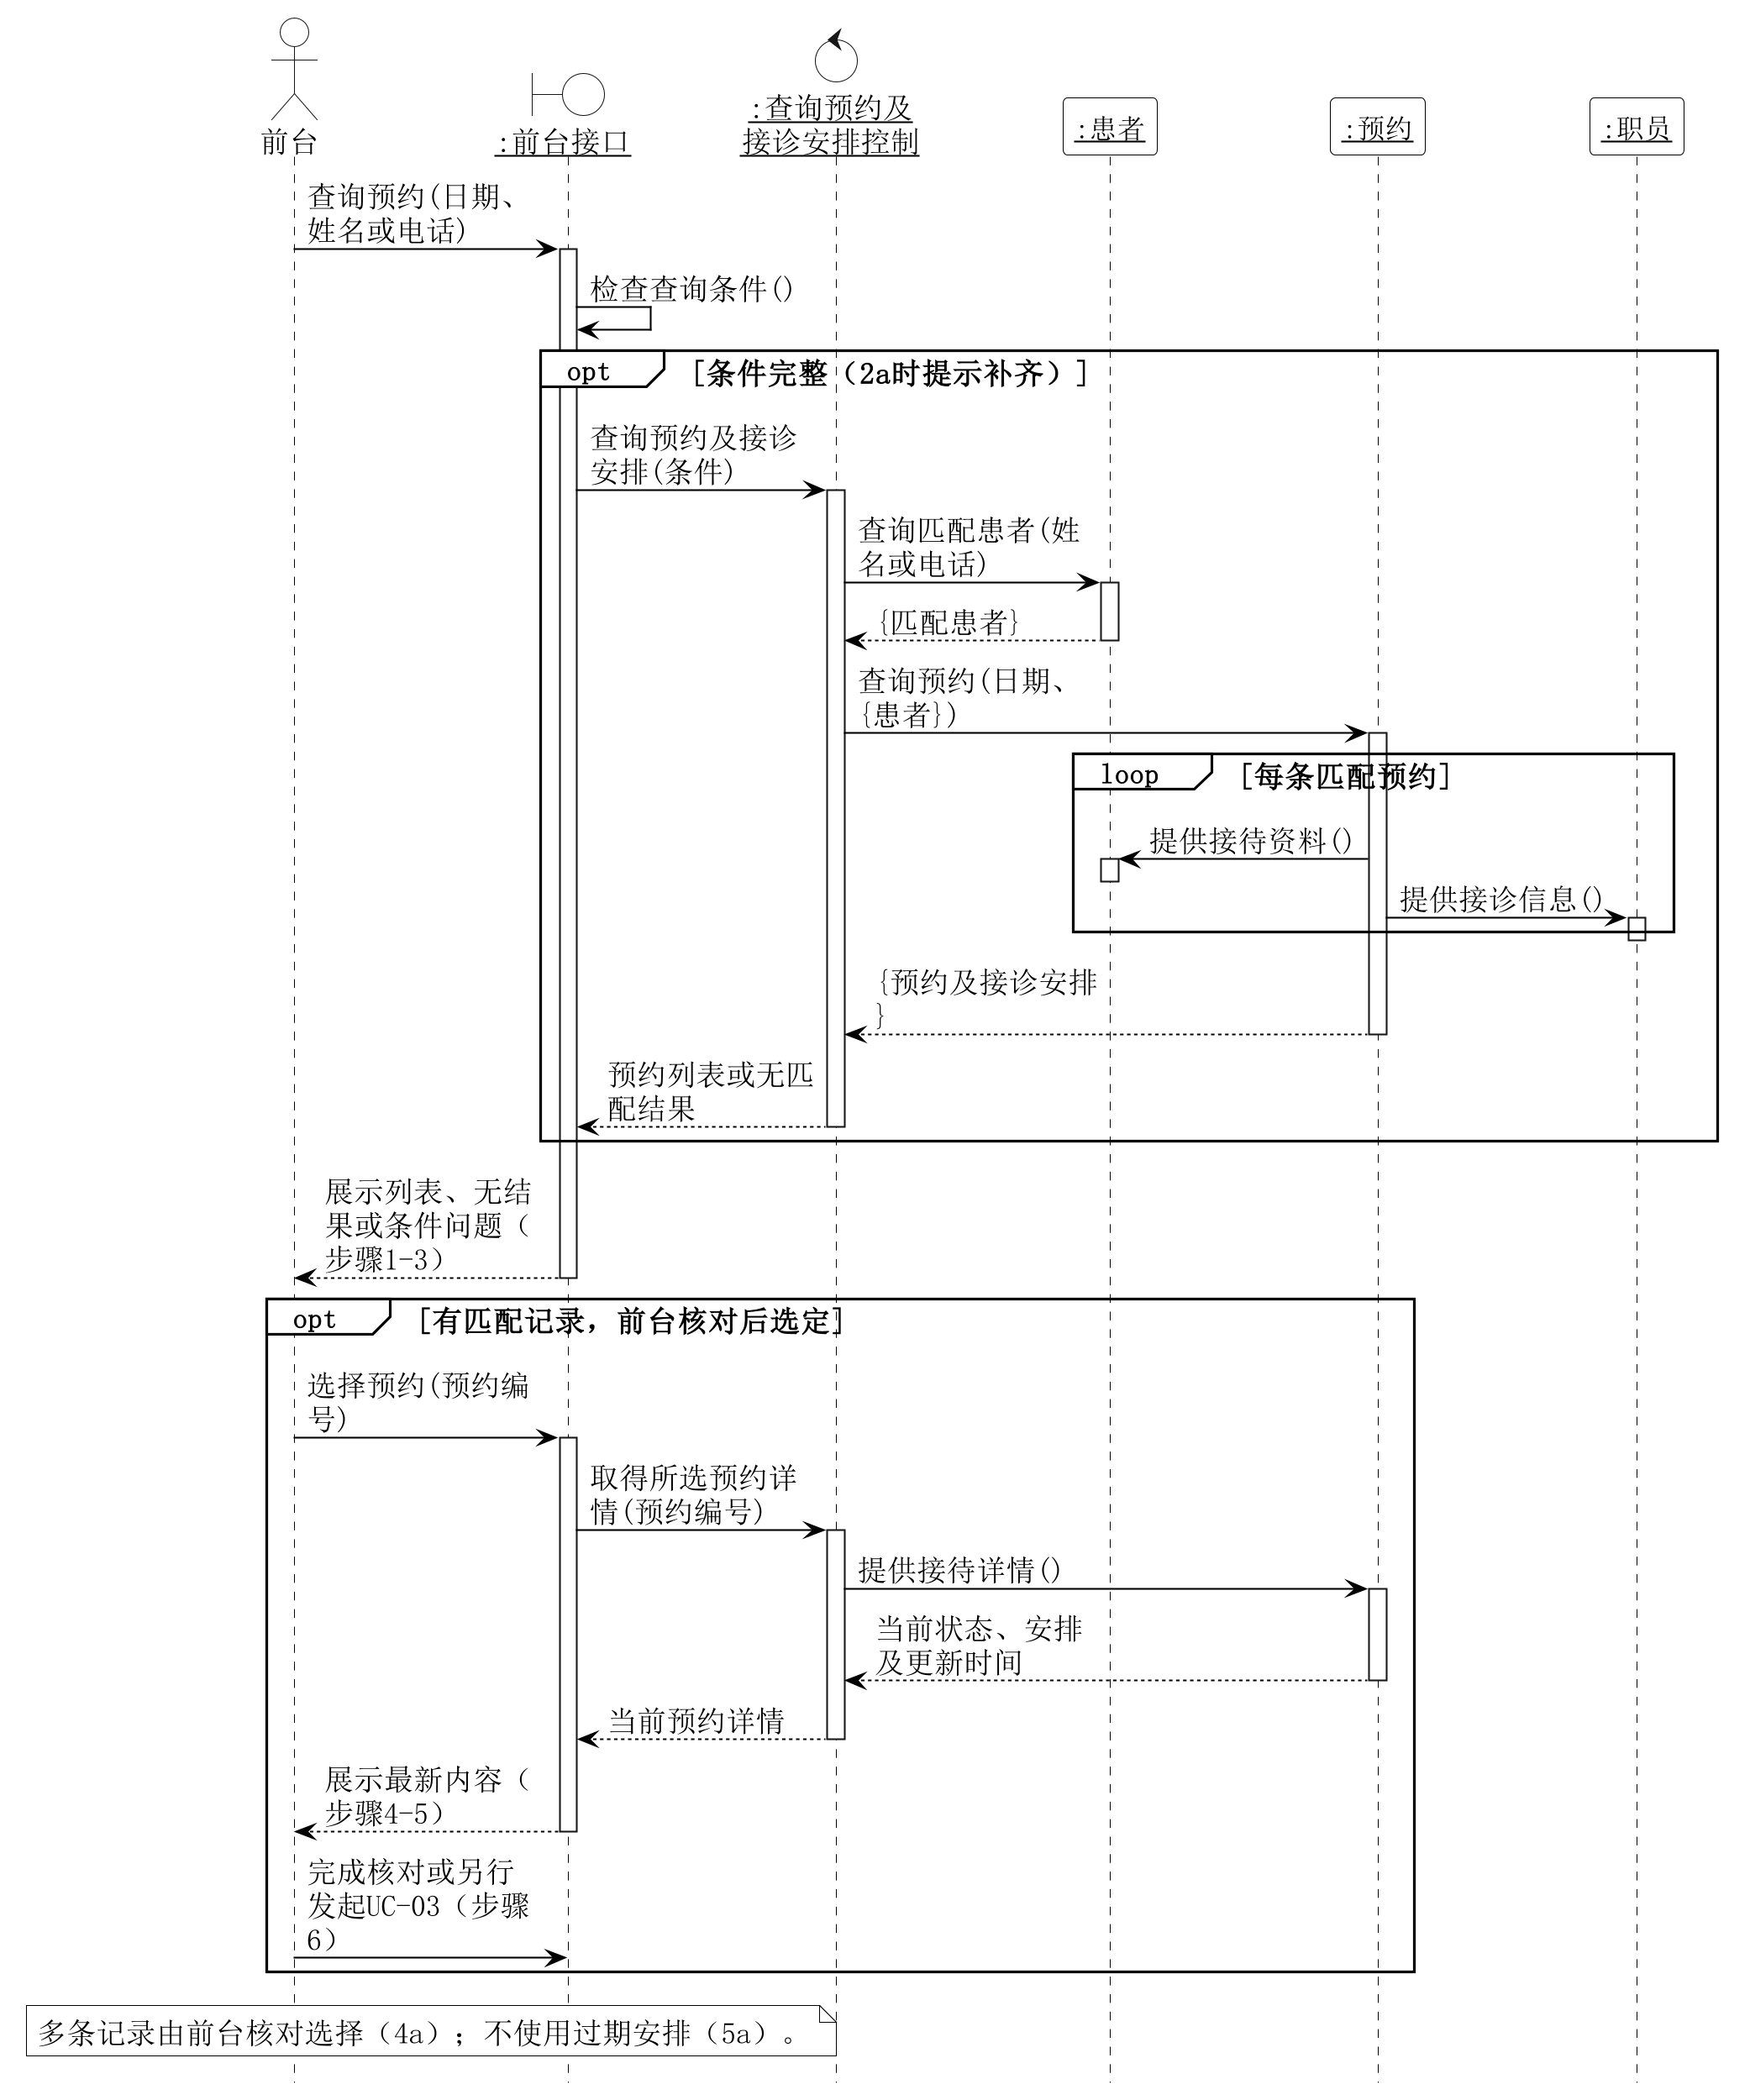
\includegraphics[width=\textwidth,height=20.4cm,keepaspectratio]{diagrams/13-02-analysis-sequence.png}
\caption{UC-02 基本路径分析序列图}
\label{fig:seq-02}
\end{figure}

\clearpage
\subsubsection{UC-03：登记到诊}
\medskip

图\ref{fig:seq-03}对应到诊登记的基本路径，合并非当日、已取消和重复提交等判断。预约判断可到诊，就诊建立并关联病历草稿；控制类协调预约、就诊及病历同时生效。前台只在患者与预约一致时提交确认，重复请求返回原对象。

\begin{figure}[!htbp]
\centering
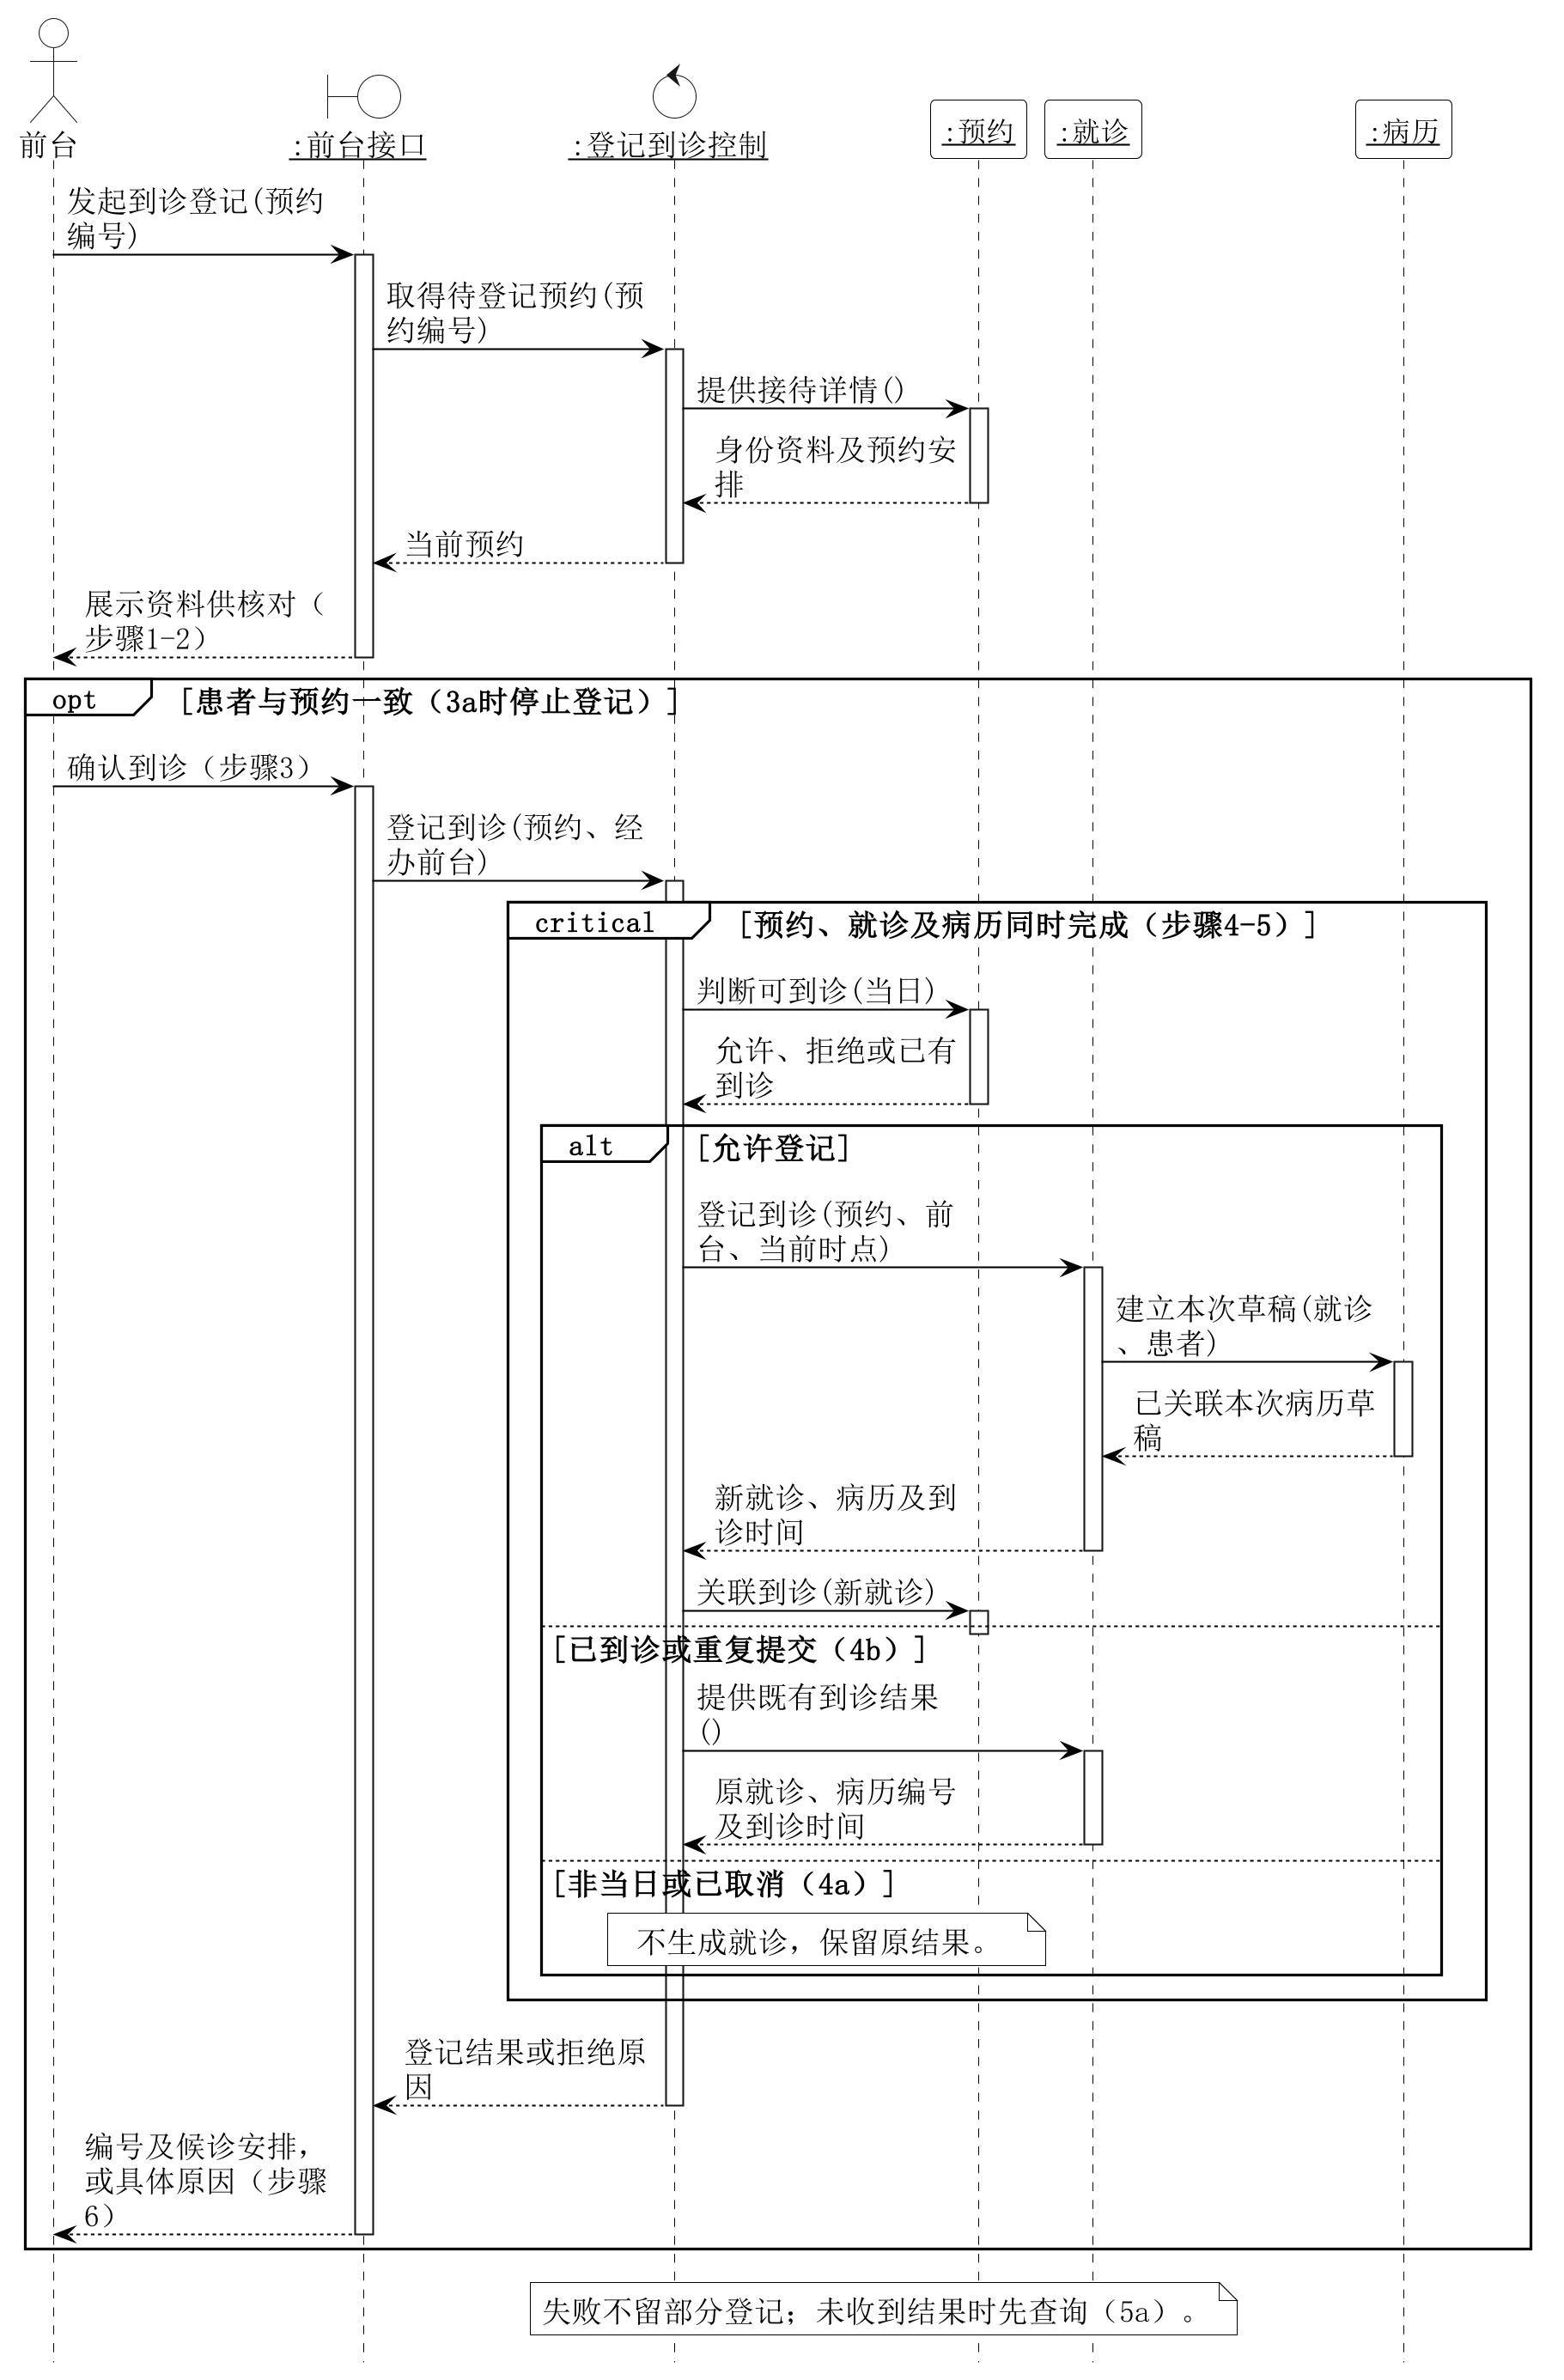
\includegraphics[width=\textwidth,height=20.4cm,keepaspectratio]{diagrams/13-03-analysis-sequence.png}
\caption{UC-03 基本路径分析序列图}
\label{fig:seq-03}
\end{figure}

\clearpage
\subsubsection{UC-04：确认诊疗项目}
\medskip

图\ref{fig:seq-04}分配实际项目确认、方案同意及拟生效数量检查责任。保存前复核当前版本；明细计价协作见图\ref{fig:seq-04-pricing}。

\begin{figure}[!htbp]
\centering
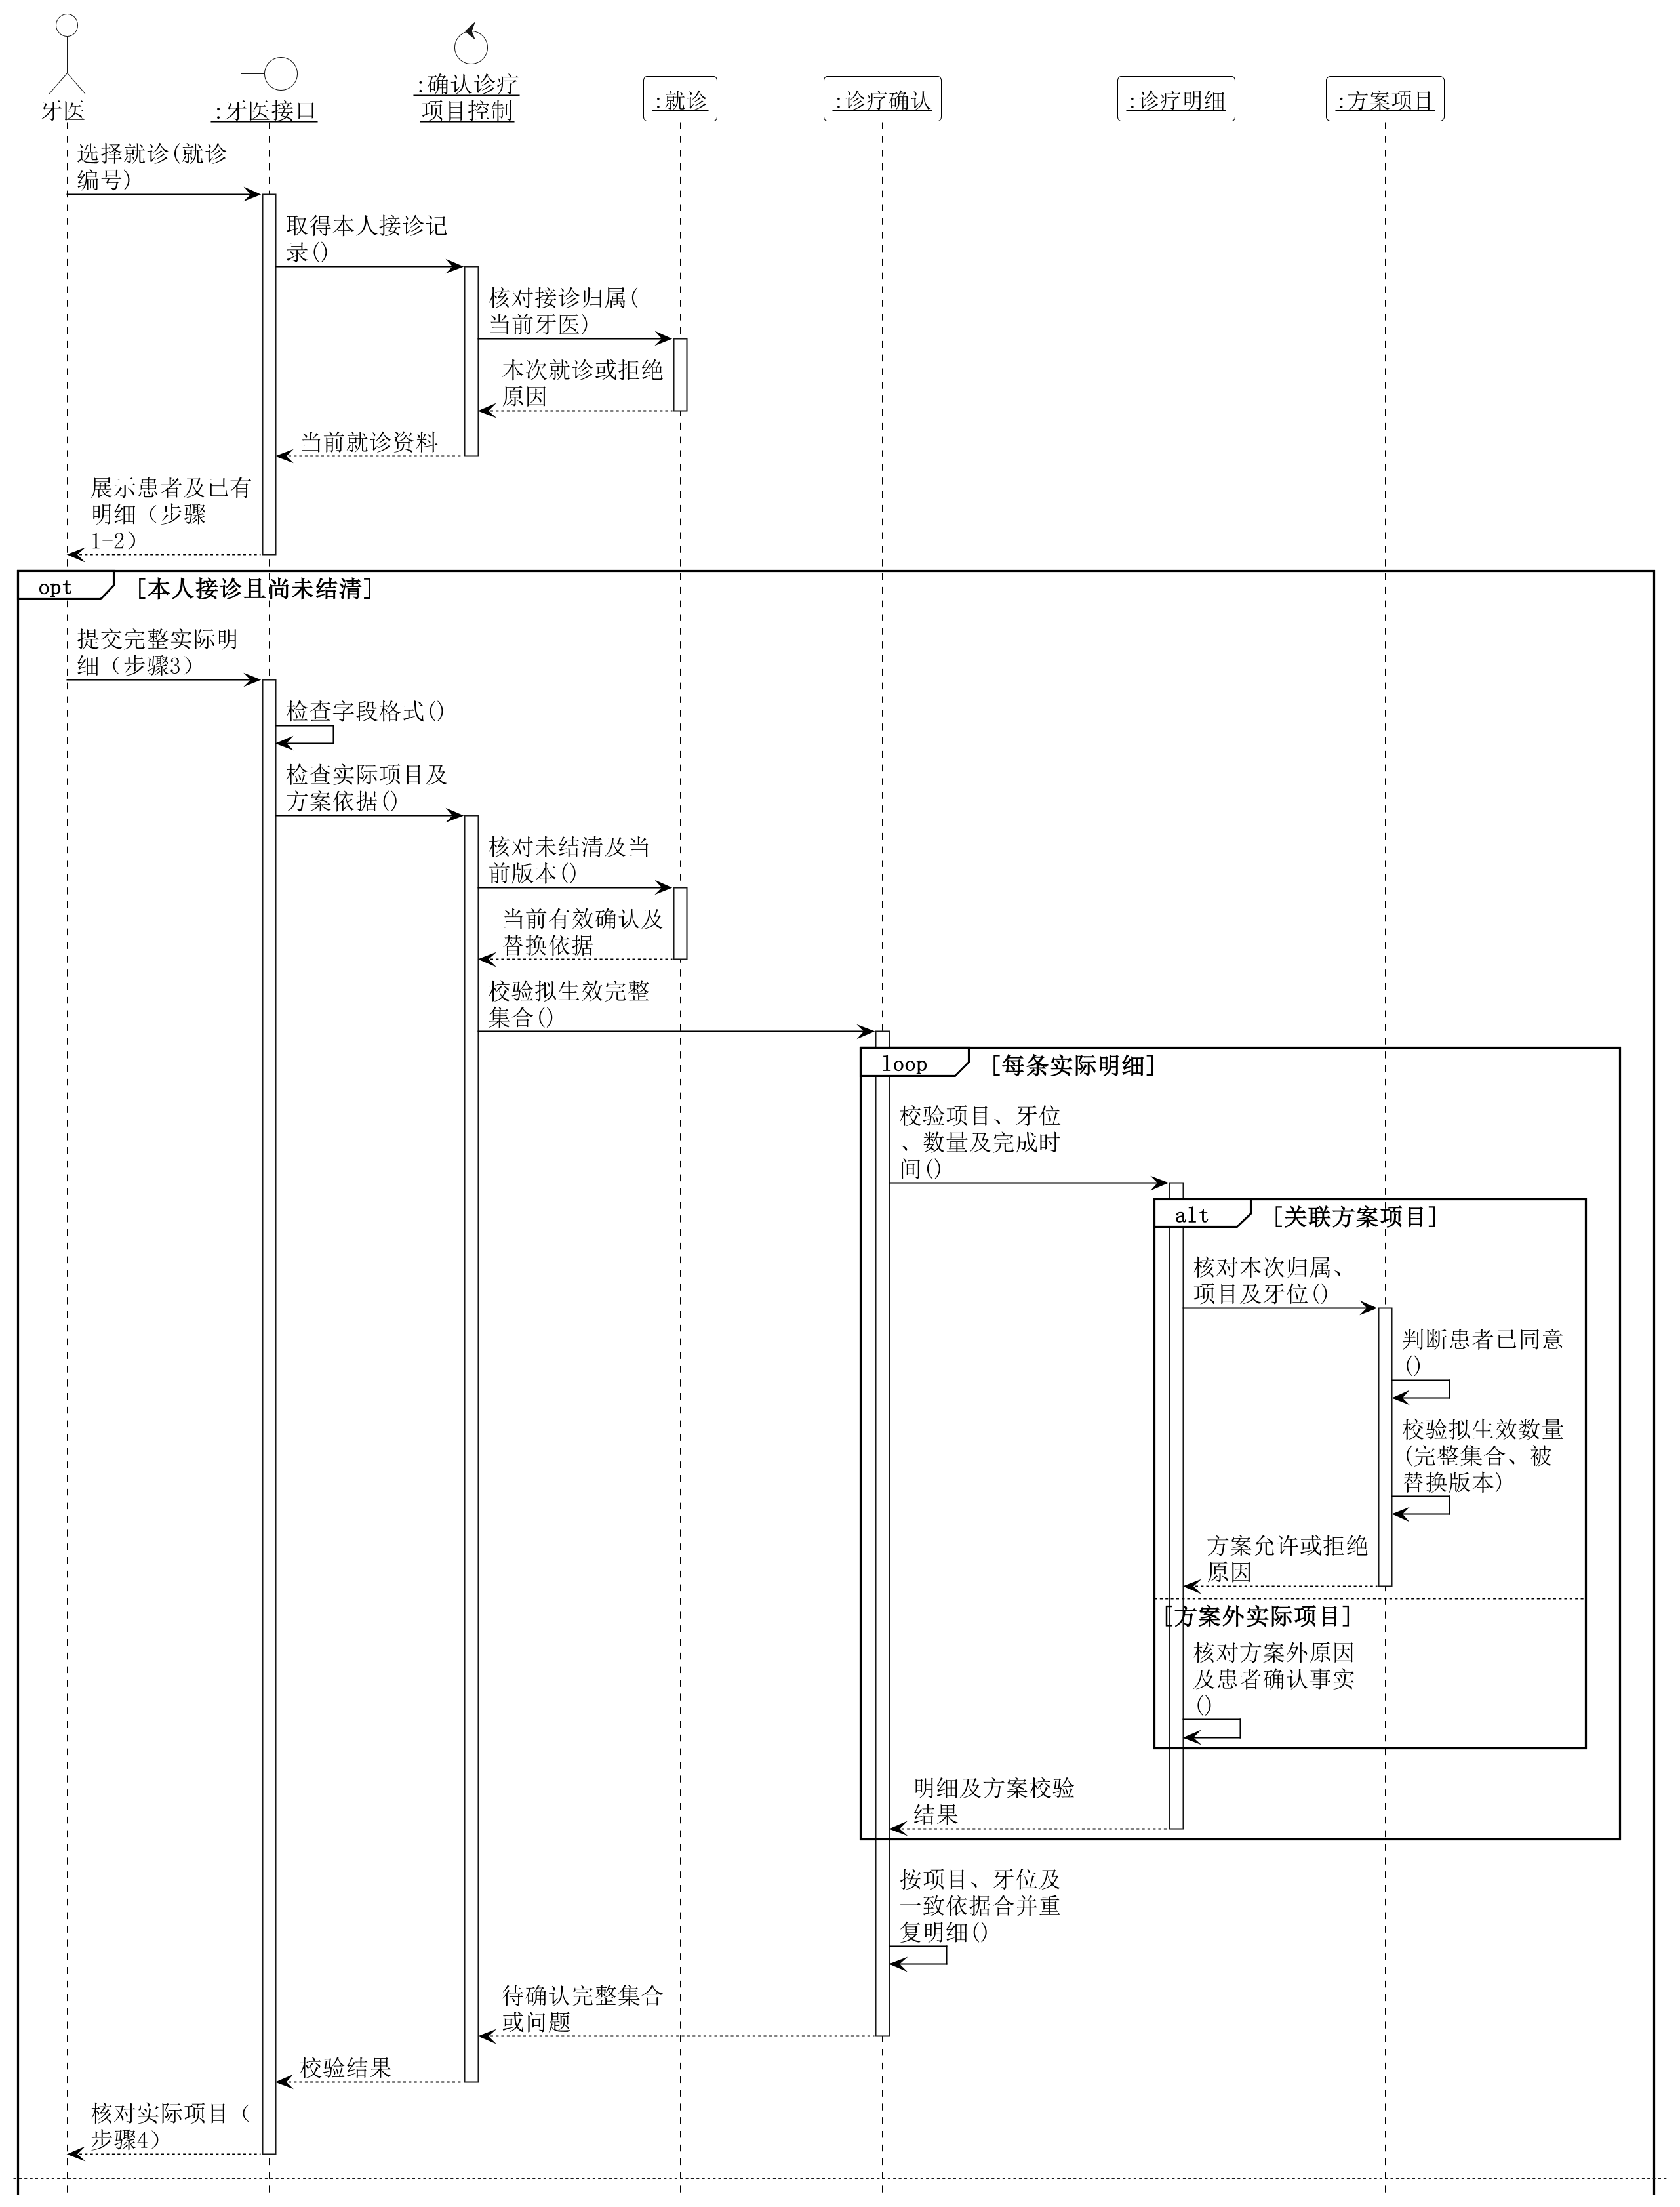
\includegraphics[width=\textwidth,height=20.4cm,keepaspectratio]{diagrams/13-04-analysis-sequence.png}
\caption{UC-04 基本路径分析序列图（扩展见图\ref{fig:seq-04-ext}）}
\label{fig:seq-04}
\end{figure}
\clearpage
\noindent\textbf{UC-04 分析序列图：基本路径（续）}
\medskip

\begin{figure}[!htbp]
\centering
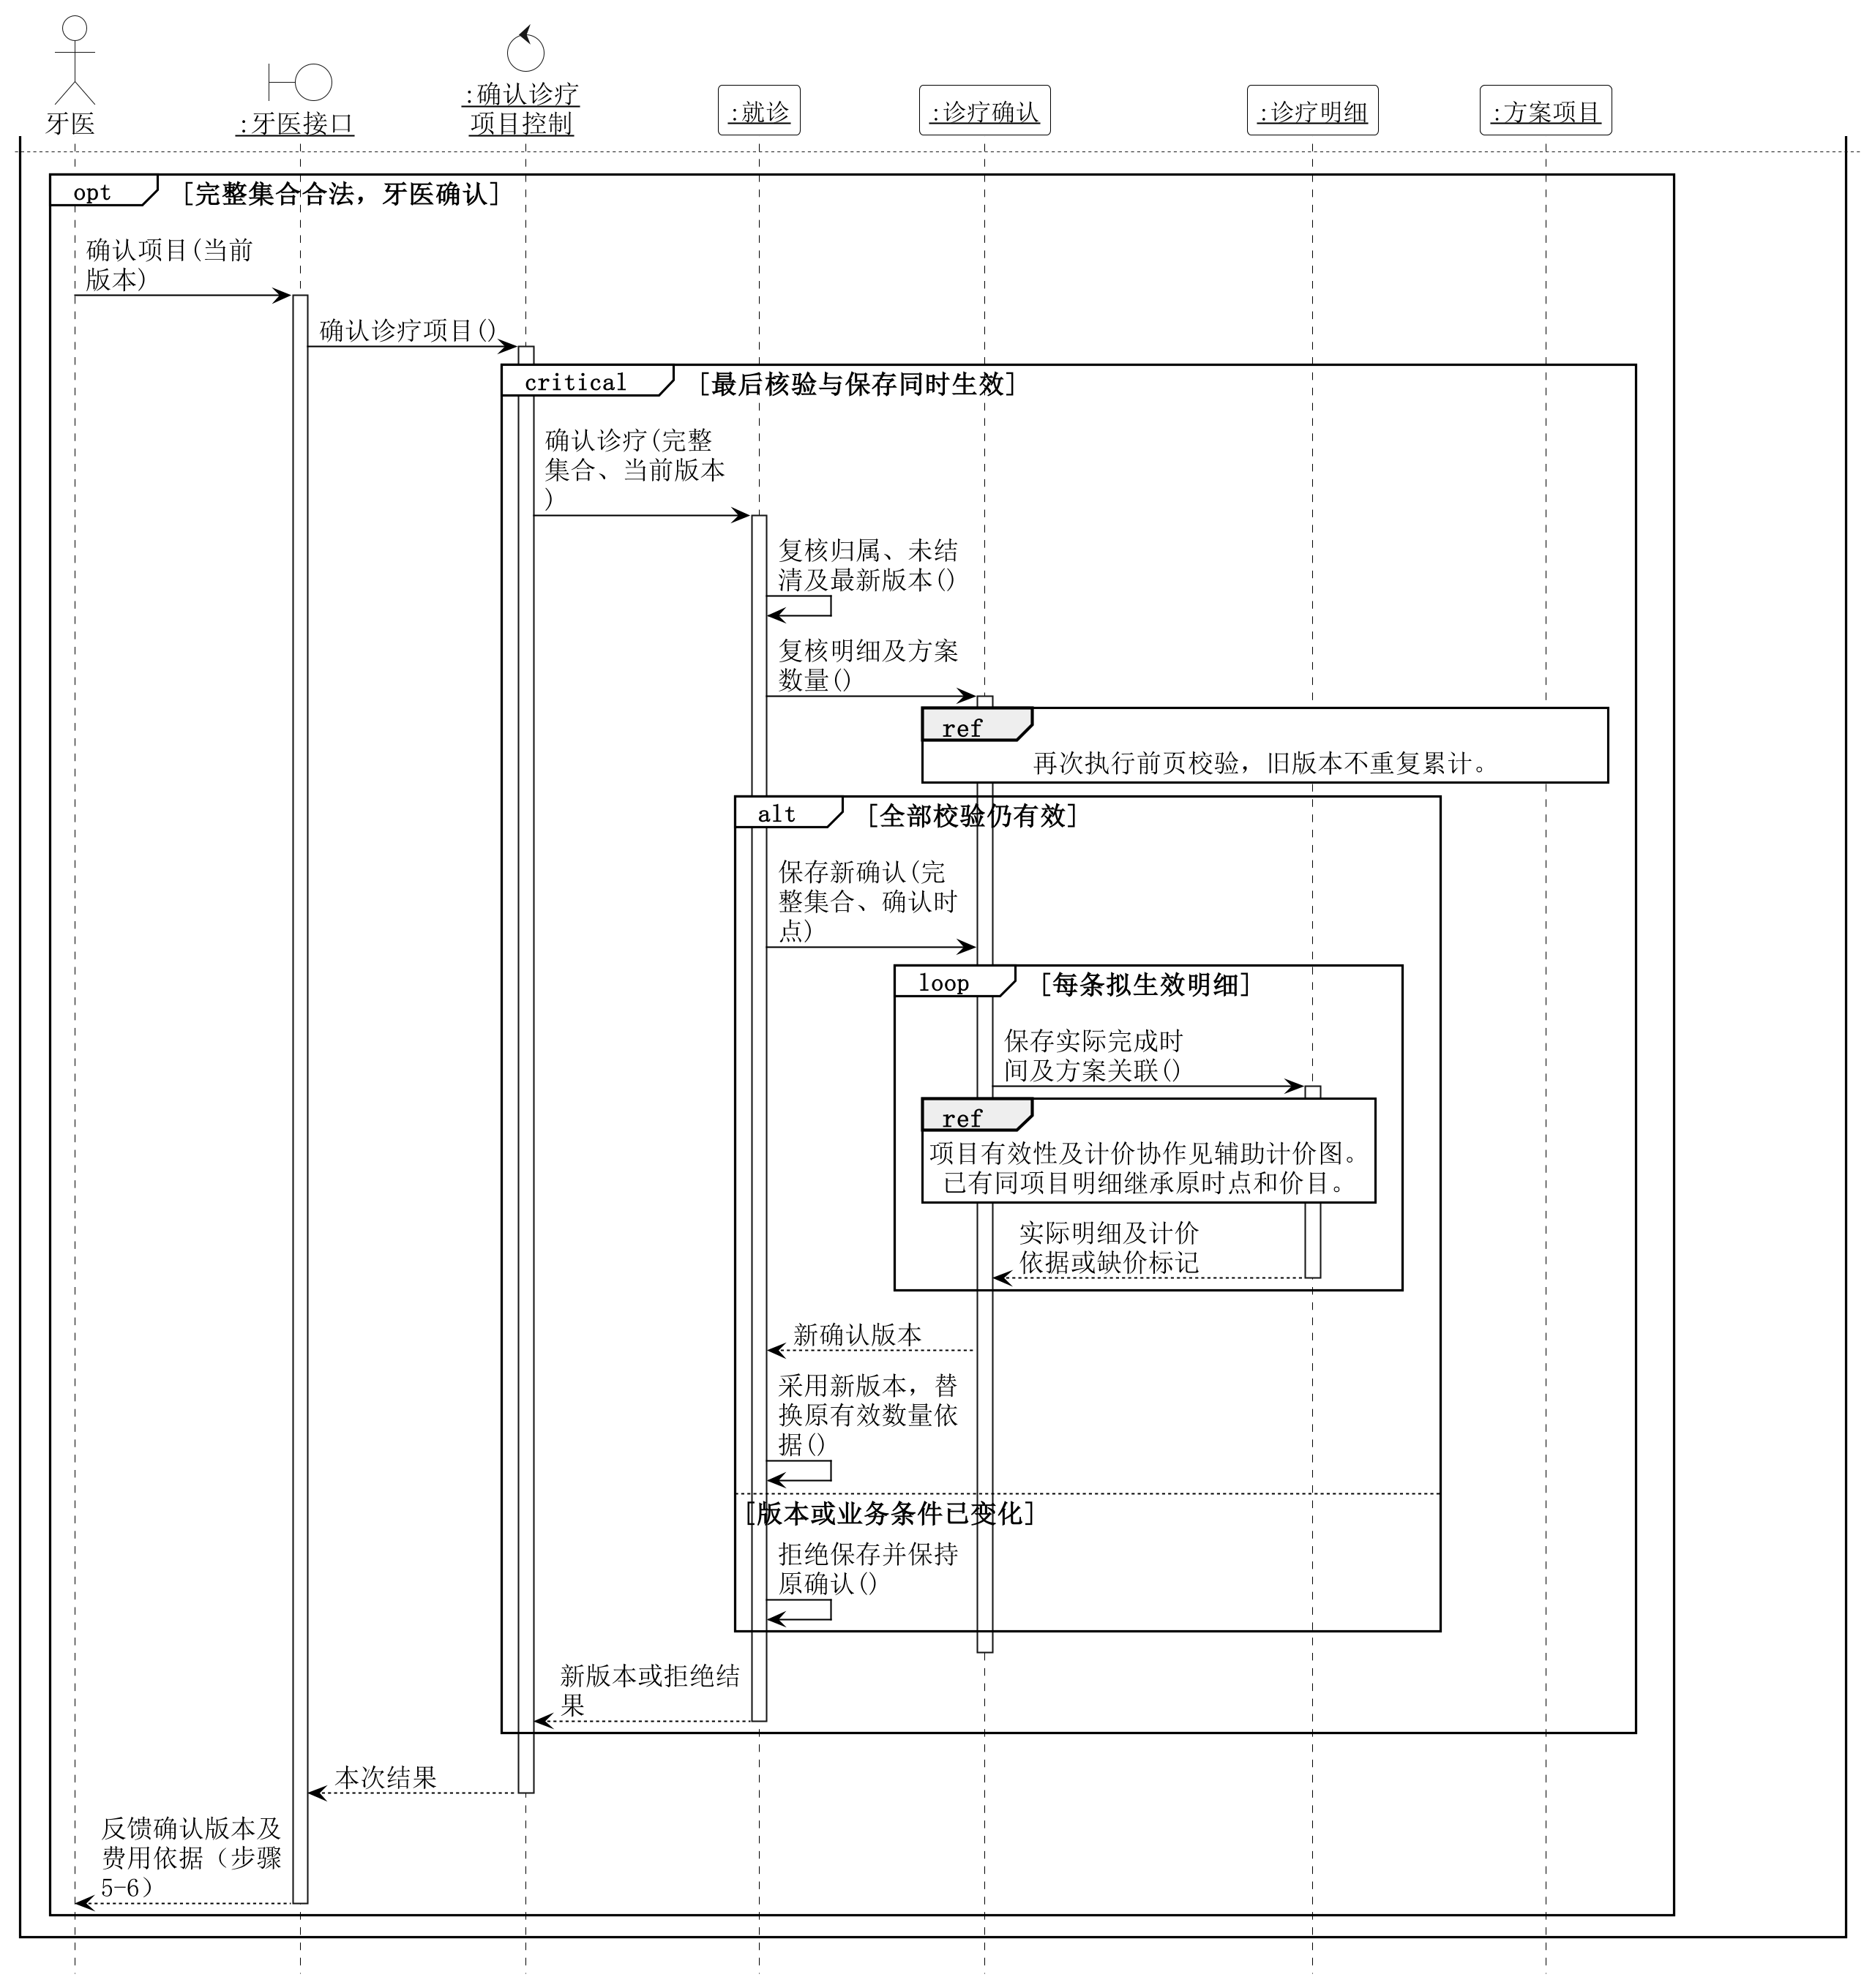
\includegraphics[width=\textwidth,height=21.3cm,keepaspectratio]{diagrams/13-04-analysis-sequence_001.png}
\par\vspace{0.5em}
{\normalsize 图\ref{fig:seq-04}（续）：UC-04 基本路径分析序列图}
\end{figure}

\clearpage
\noindent\textbf{UC-04 分析序列图：更正已确认诊疗项目}
\medskip

图\ref{fig:seq-04-ext}对应4b、6a。更正复核完整明细及方案，计价见图\ref{fig:seq-04-pricing}；新版本替换原版本，保留历史并重算有效数量，旧费用核对依据失效。

\begin{figure}[!htbp]
\centering
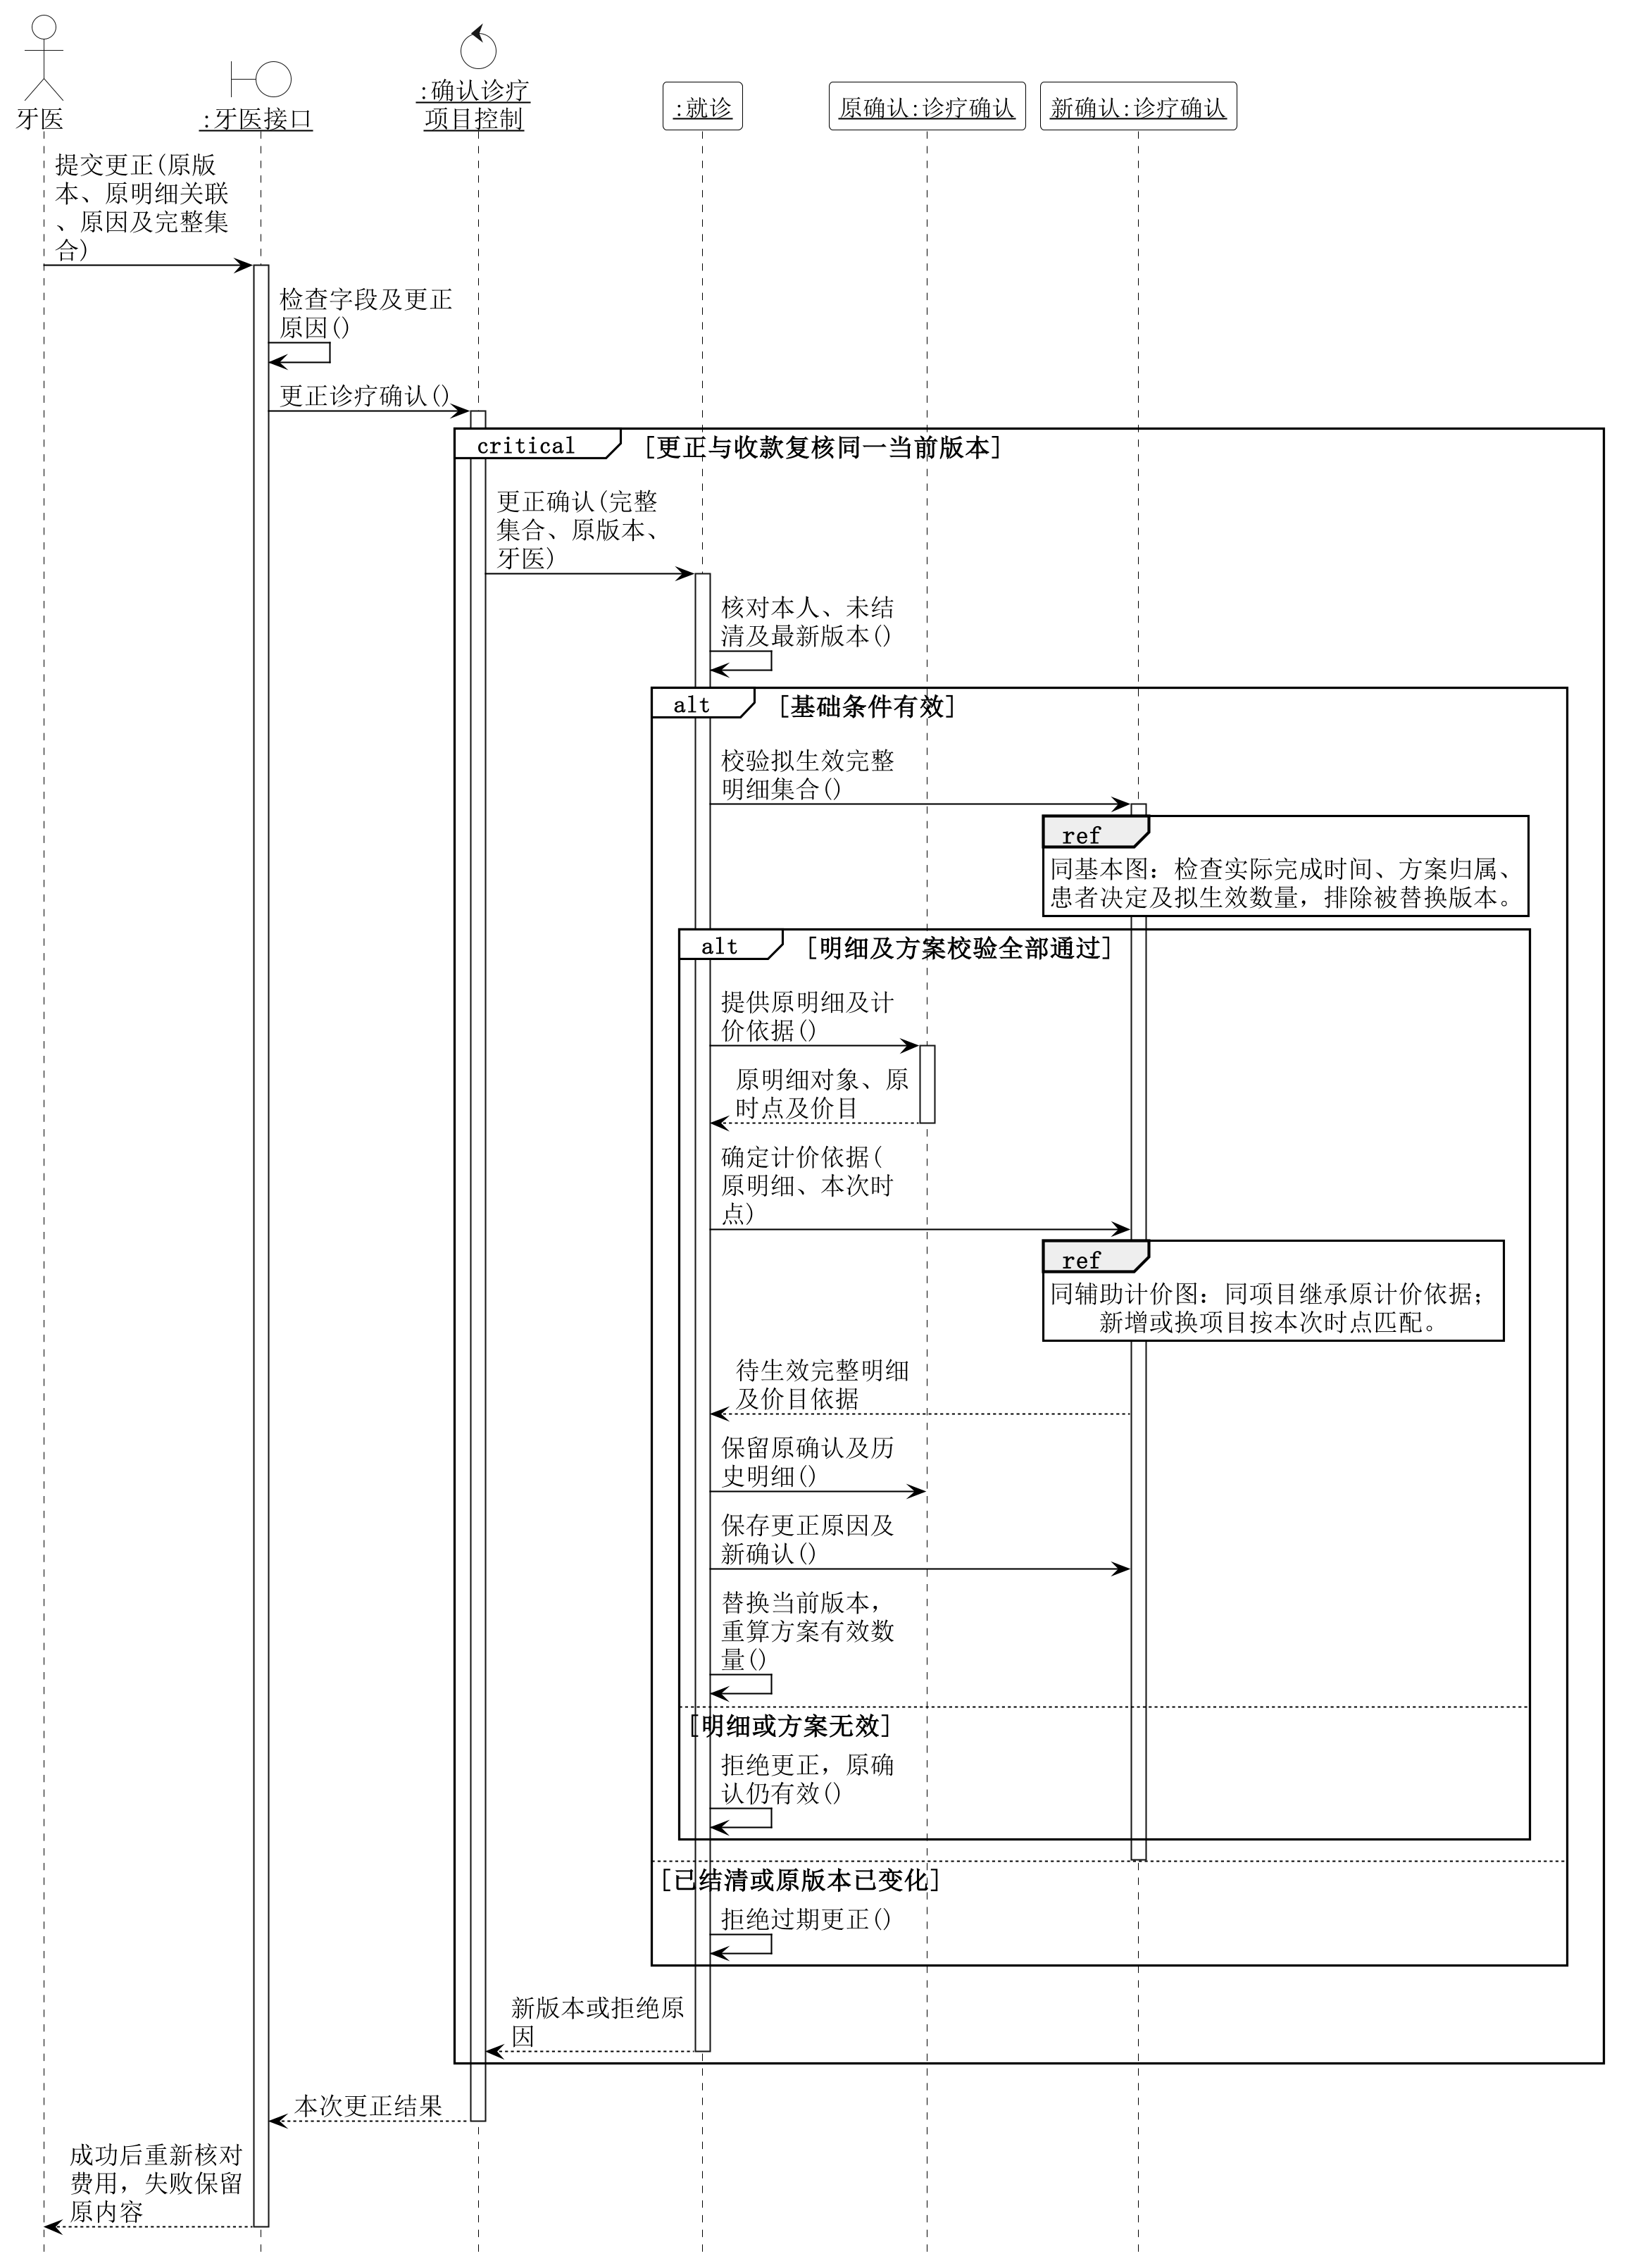
\includegraphics[width=\textwidth,height=20.4cm,keepaspectratio]{diagrams/13-04a-analysis-sequence.png}
\caption{UC-04 更正已确认诊疗项目分析序列图}
\label{fig:seq-04-ext}
\end{figure}

\clearpage
\noindent\textbf{UC-04 分析序列图：明细计价协作}
\medskip

图\ref{fig:seq-04-pricing}由诊疗确认逐条组织明细计价。已有同项目明细通过原明细关联继承价格依据；新增或更换项目使用本次确认时点。原缺价行仍按保存的计价时点补齐，实际完成时间用于项目统计。
\begin{figure}[!htbp]
\centering
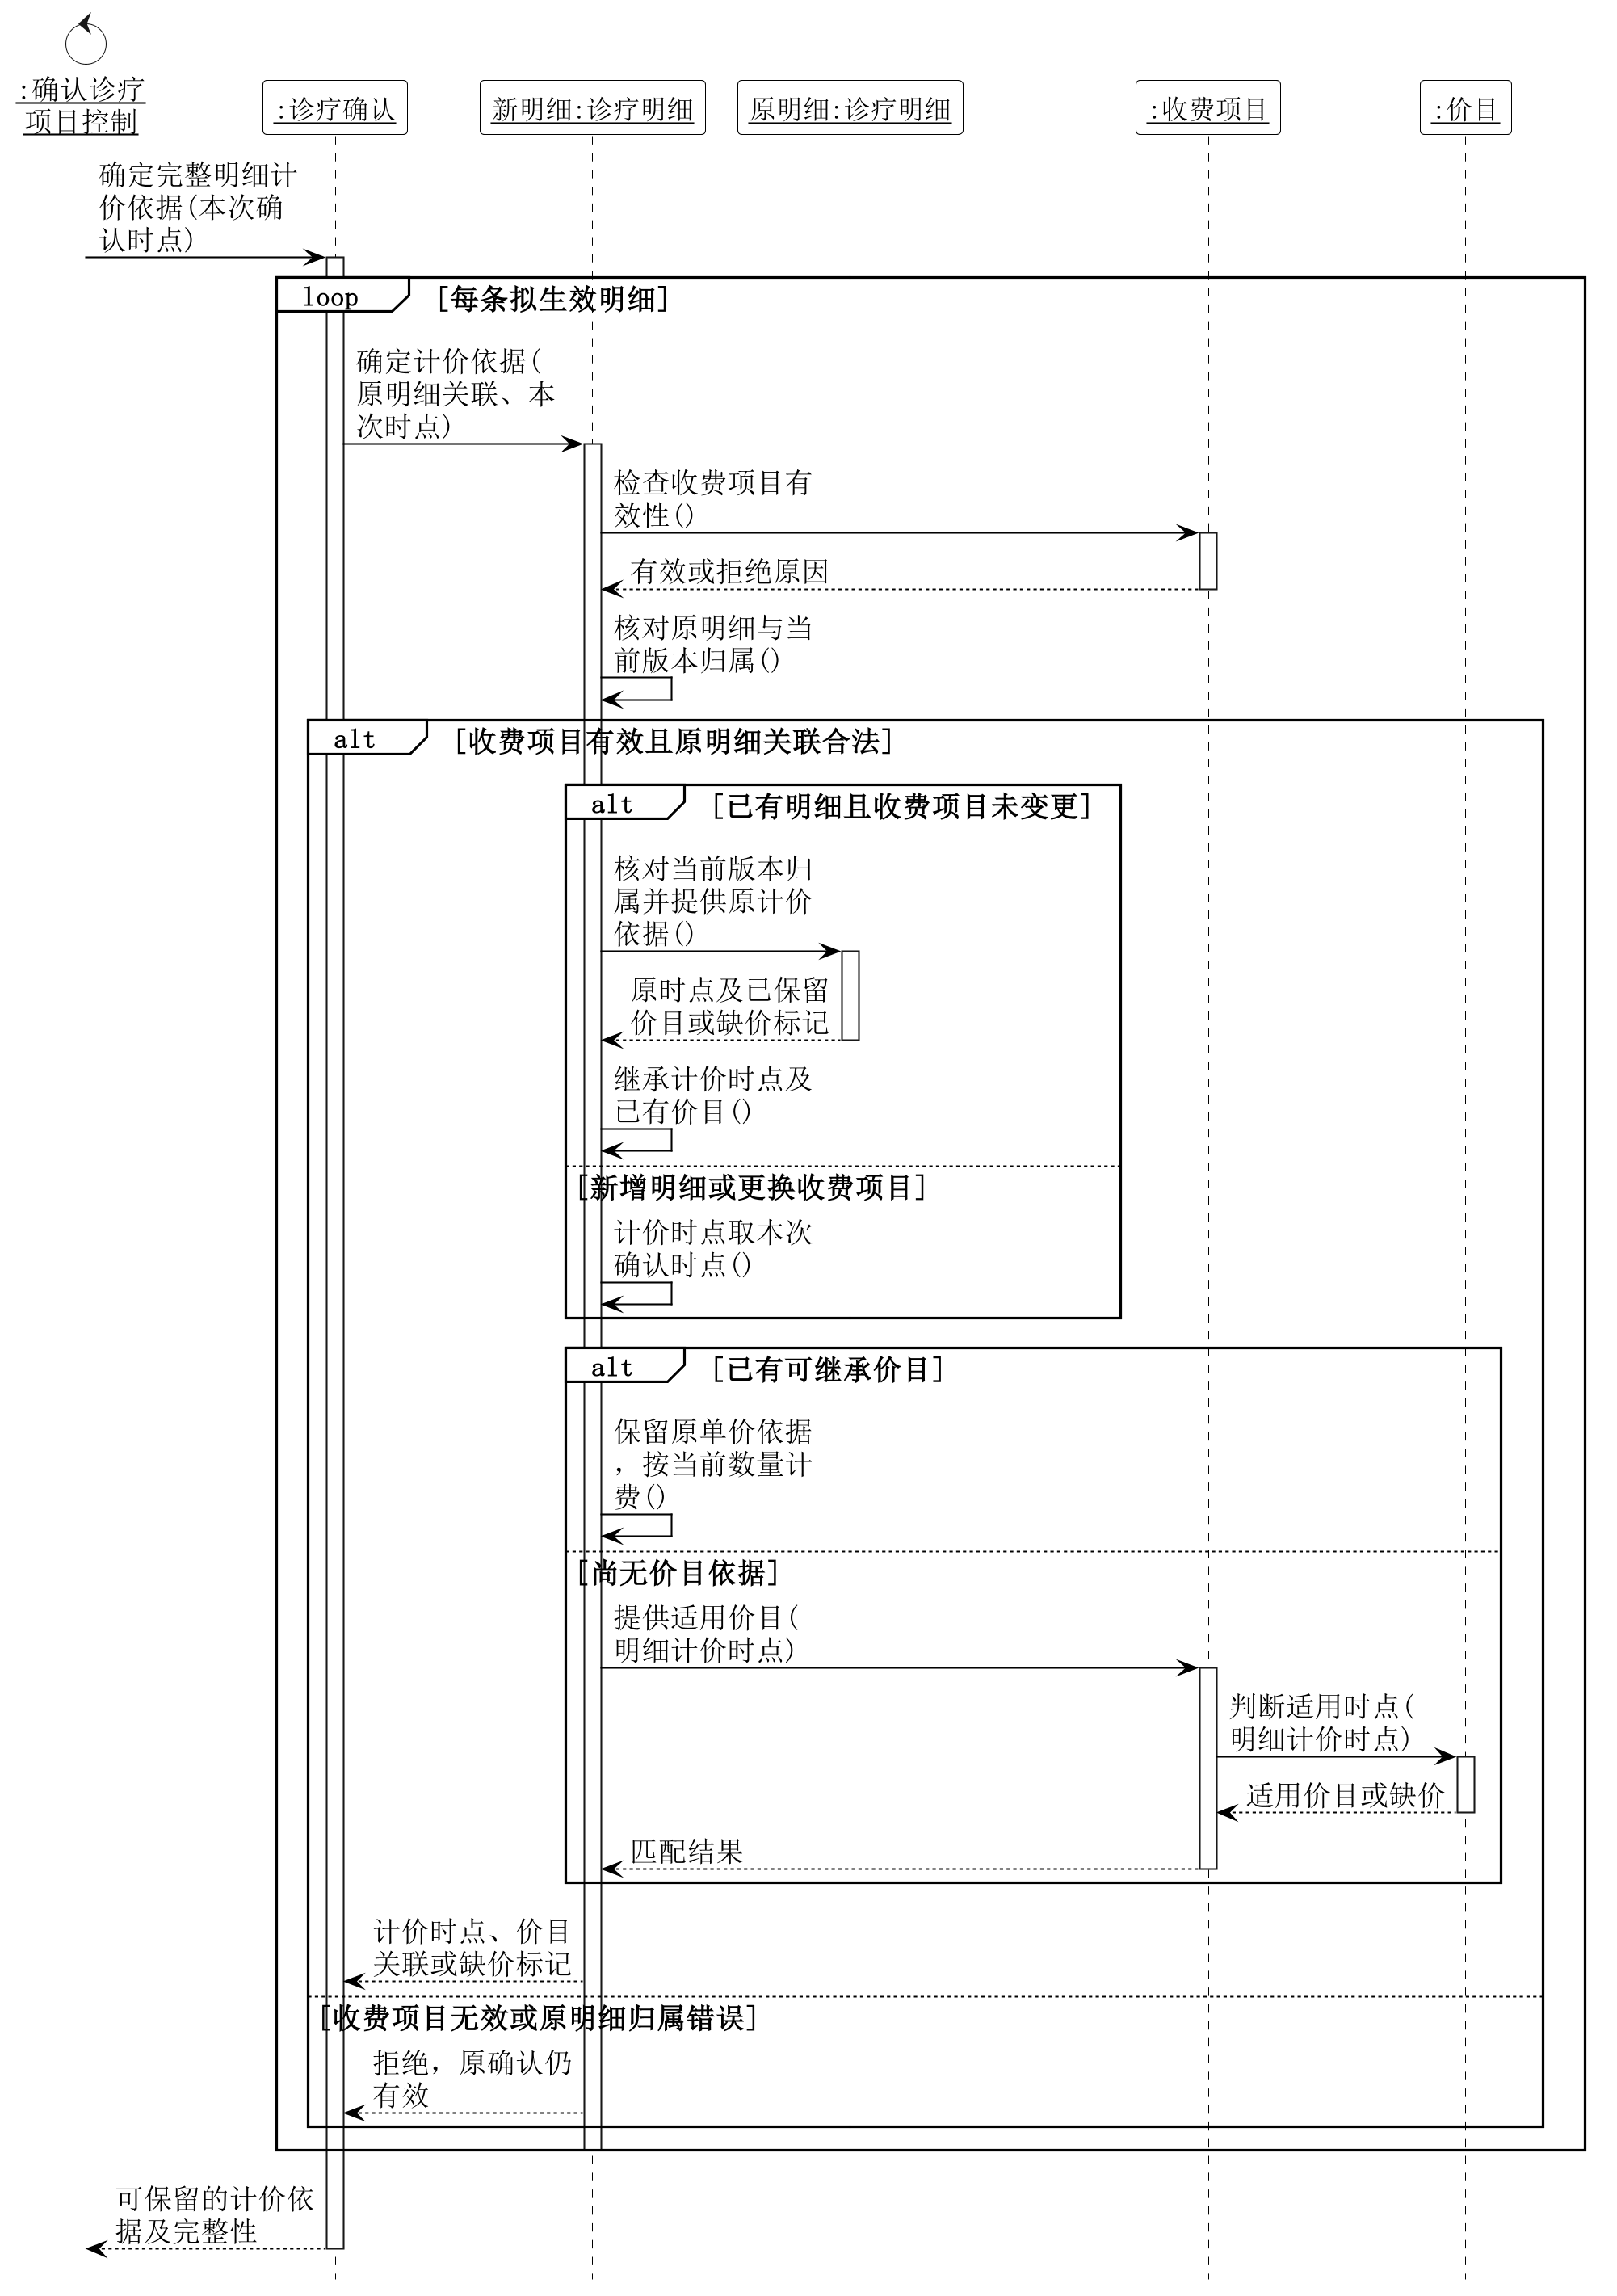
\includegraphics[width=\textwidth,height=19.5cm,keepaspectratio]{diagrams/13-04b-analysis-pricing.png}
\caption{UC-04 明细计价分析序列图}
\label{fig:seq-04-pricing}
\end{figure}
\clearpage
\subsubsection{UC-05：维护收费价目}
\medskip

图\ref{fig:seq-05}对应价目维护的基本路径。收费人员接口检查格式与负责人确认信息；收费项目组织价目方案，价目判断适用区间是否重叠。保存前重新核对当前内容，保证同一项目在同一时点至多一个适用价格。

\begin{figure}[!htbp]
\centering
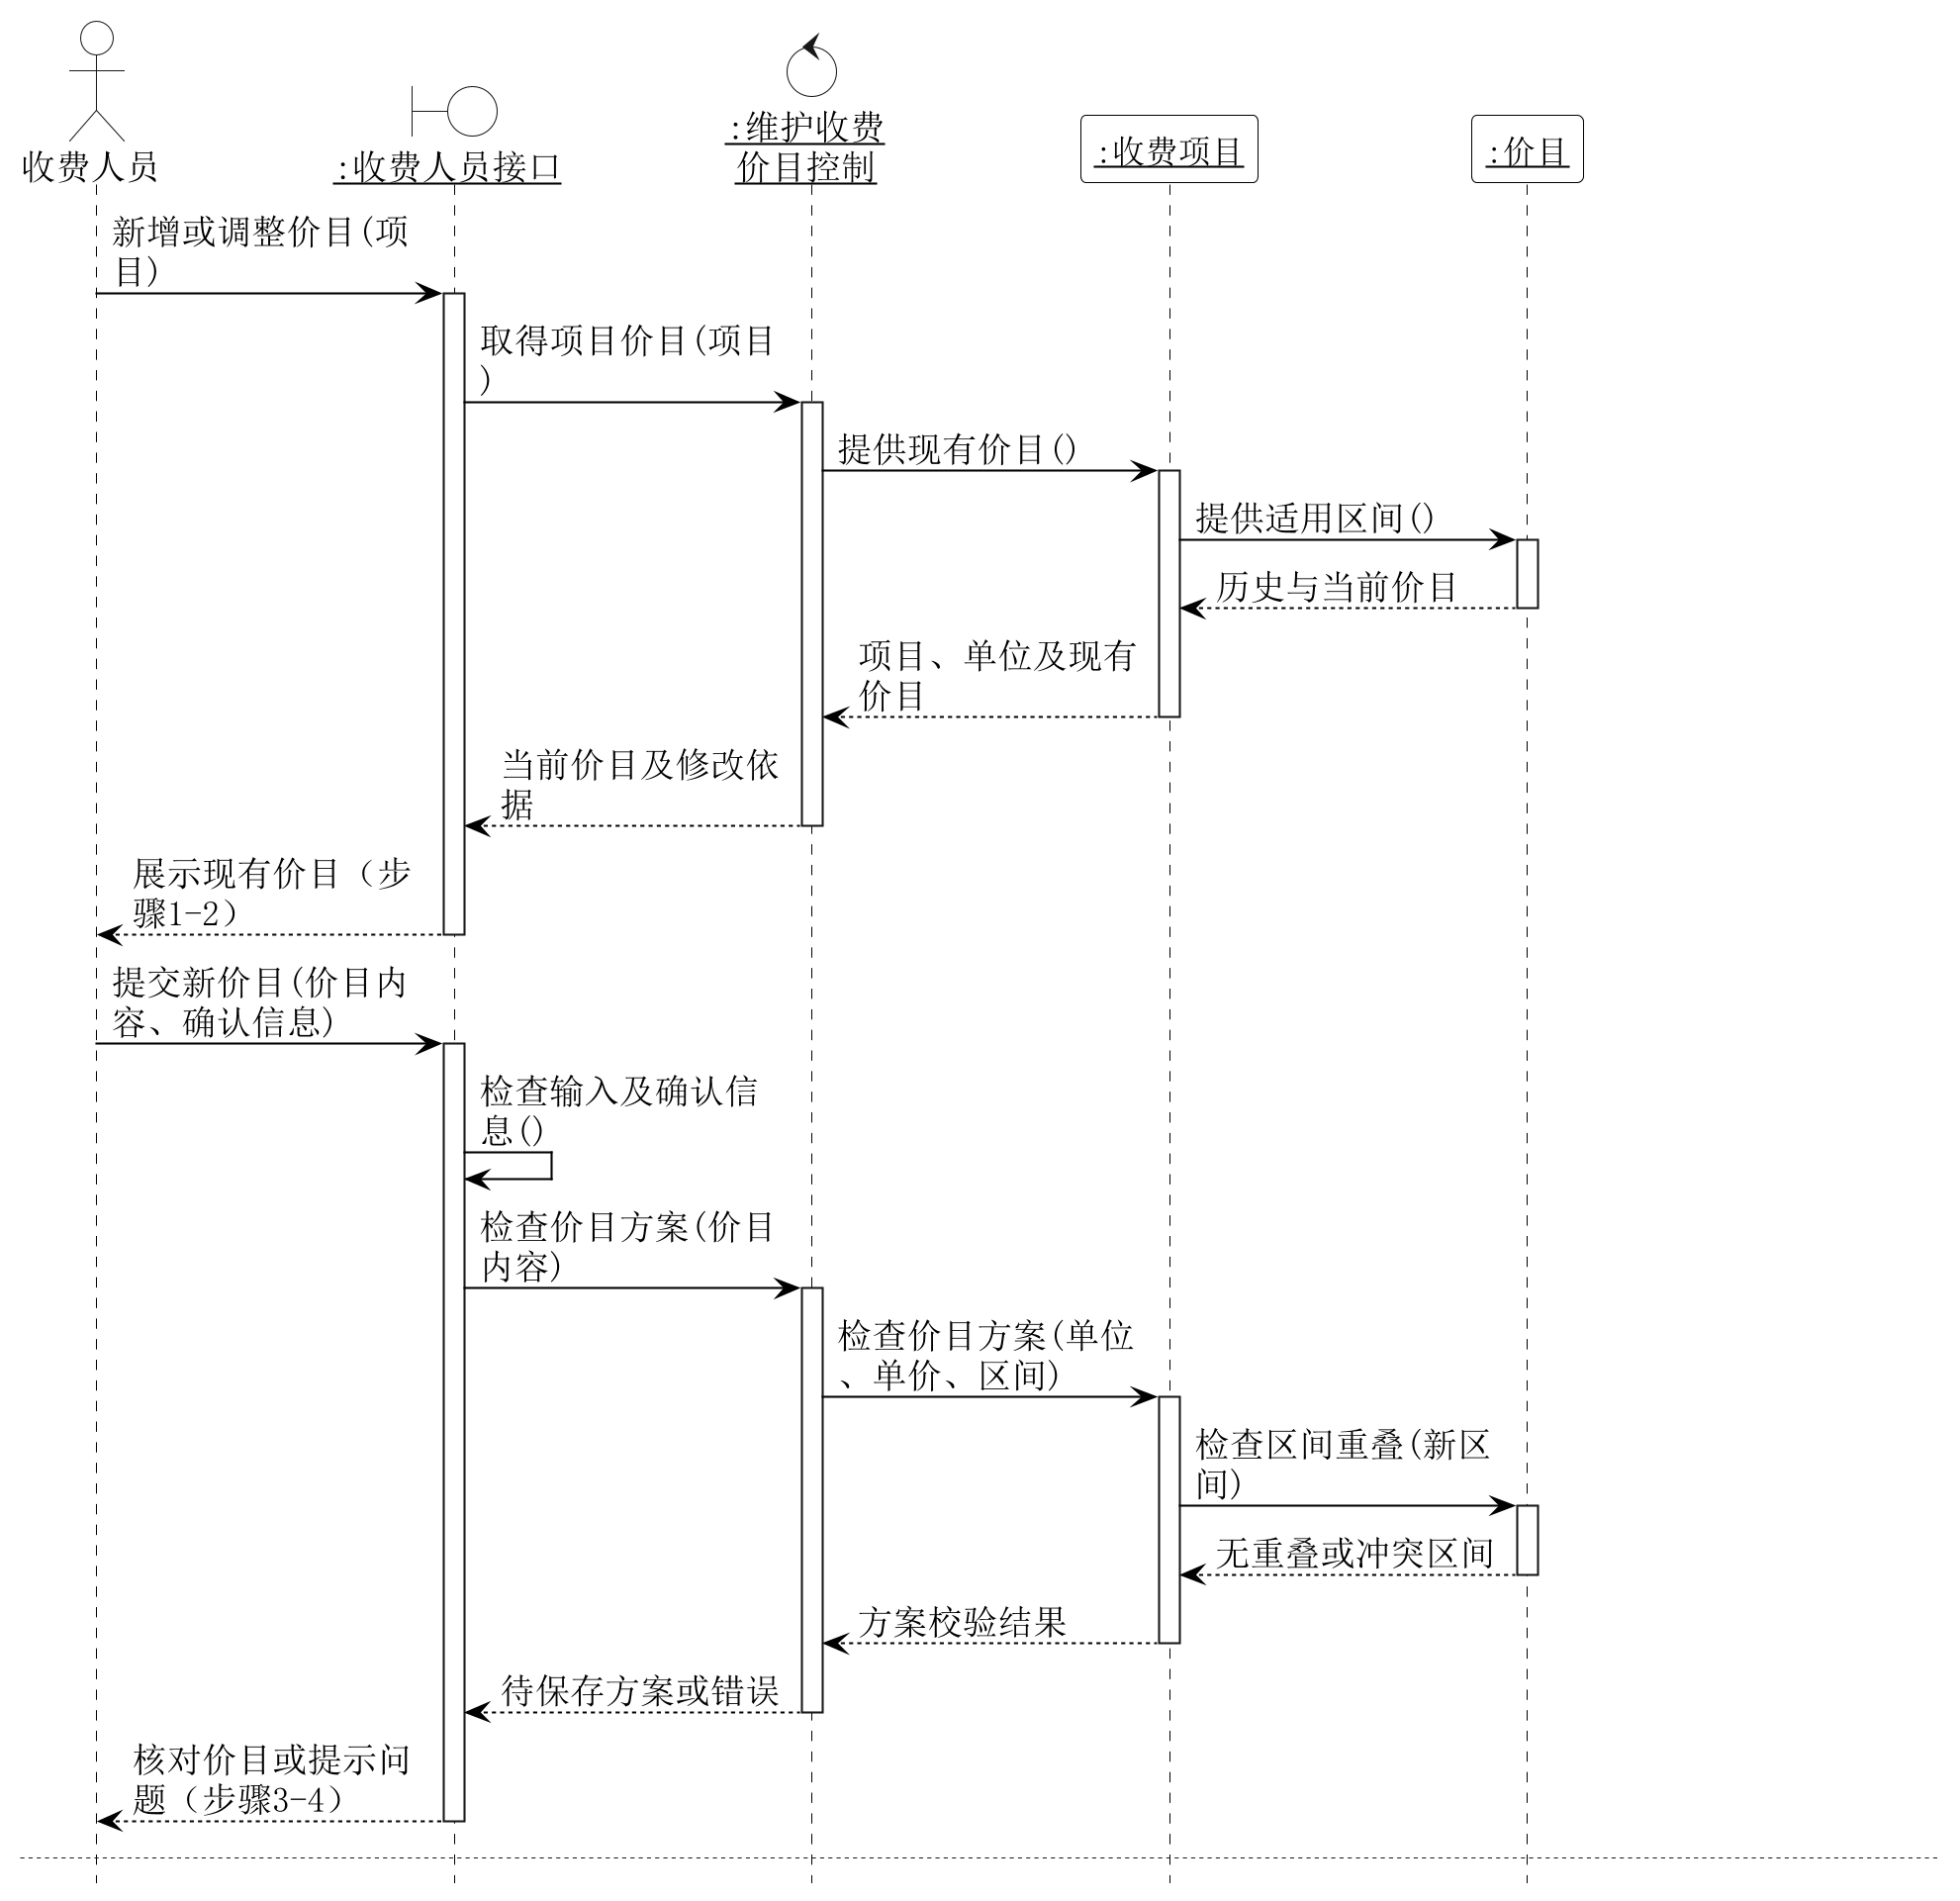
\includegraphics[width=\textwidth,height=20.4cm,keepaspectratio]{diagrams/13-05-analysis-sequence.png}
\caption{UC-05 基本路径分析序列图（扩展见图\ref{fig:seq-05-ext}）}
\label{fig:seq-05}
\end{figure}
\clearpage
\noindent\textbf{UC-05 分析序列图：基本路径（续）}
\medskip

\begin{figure}[!htbp]
\centering
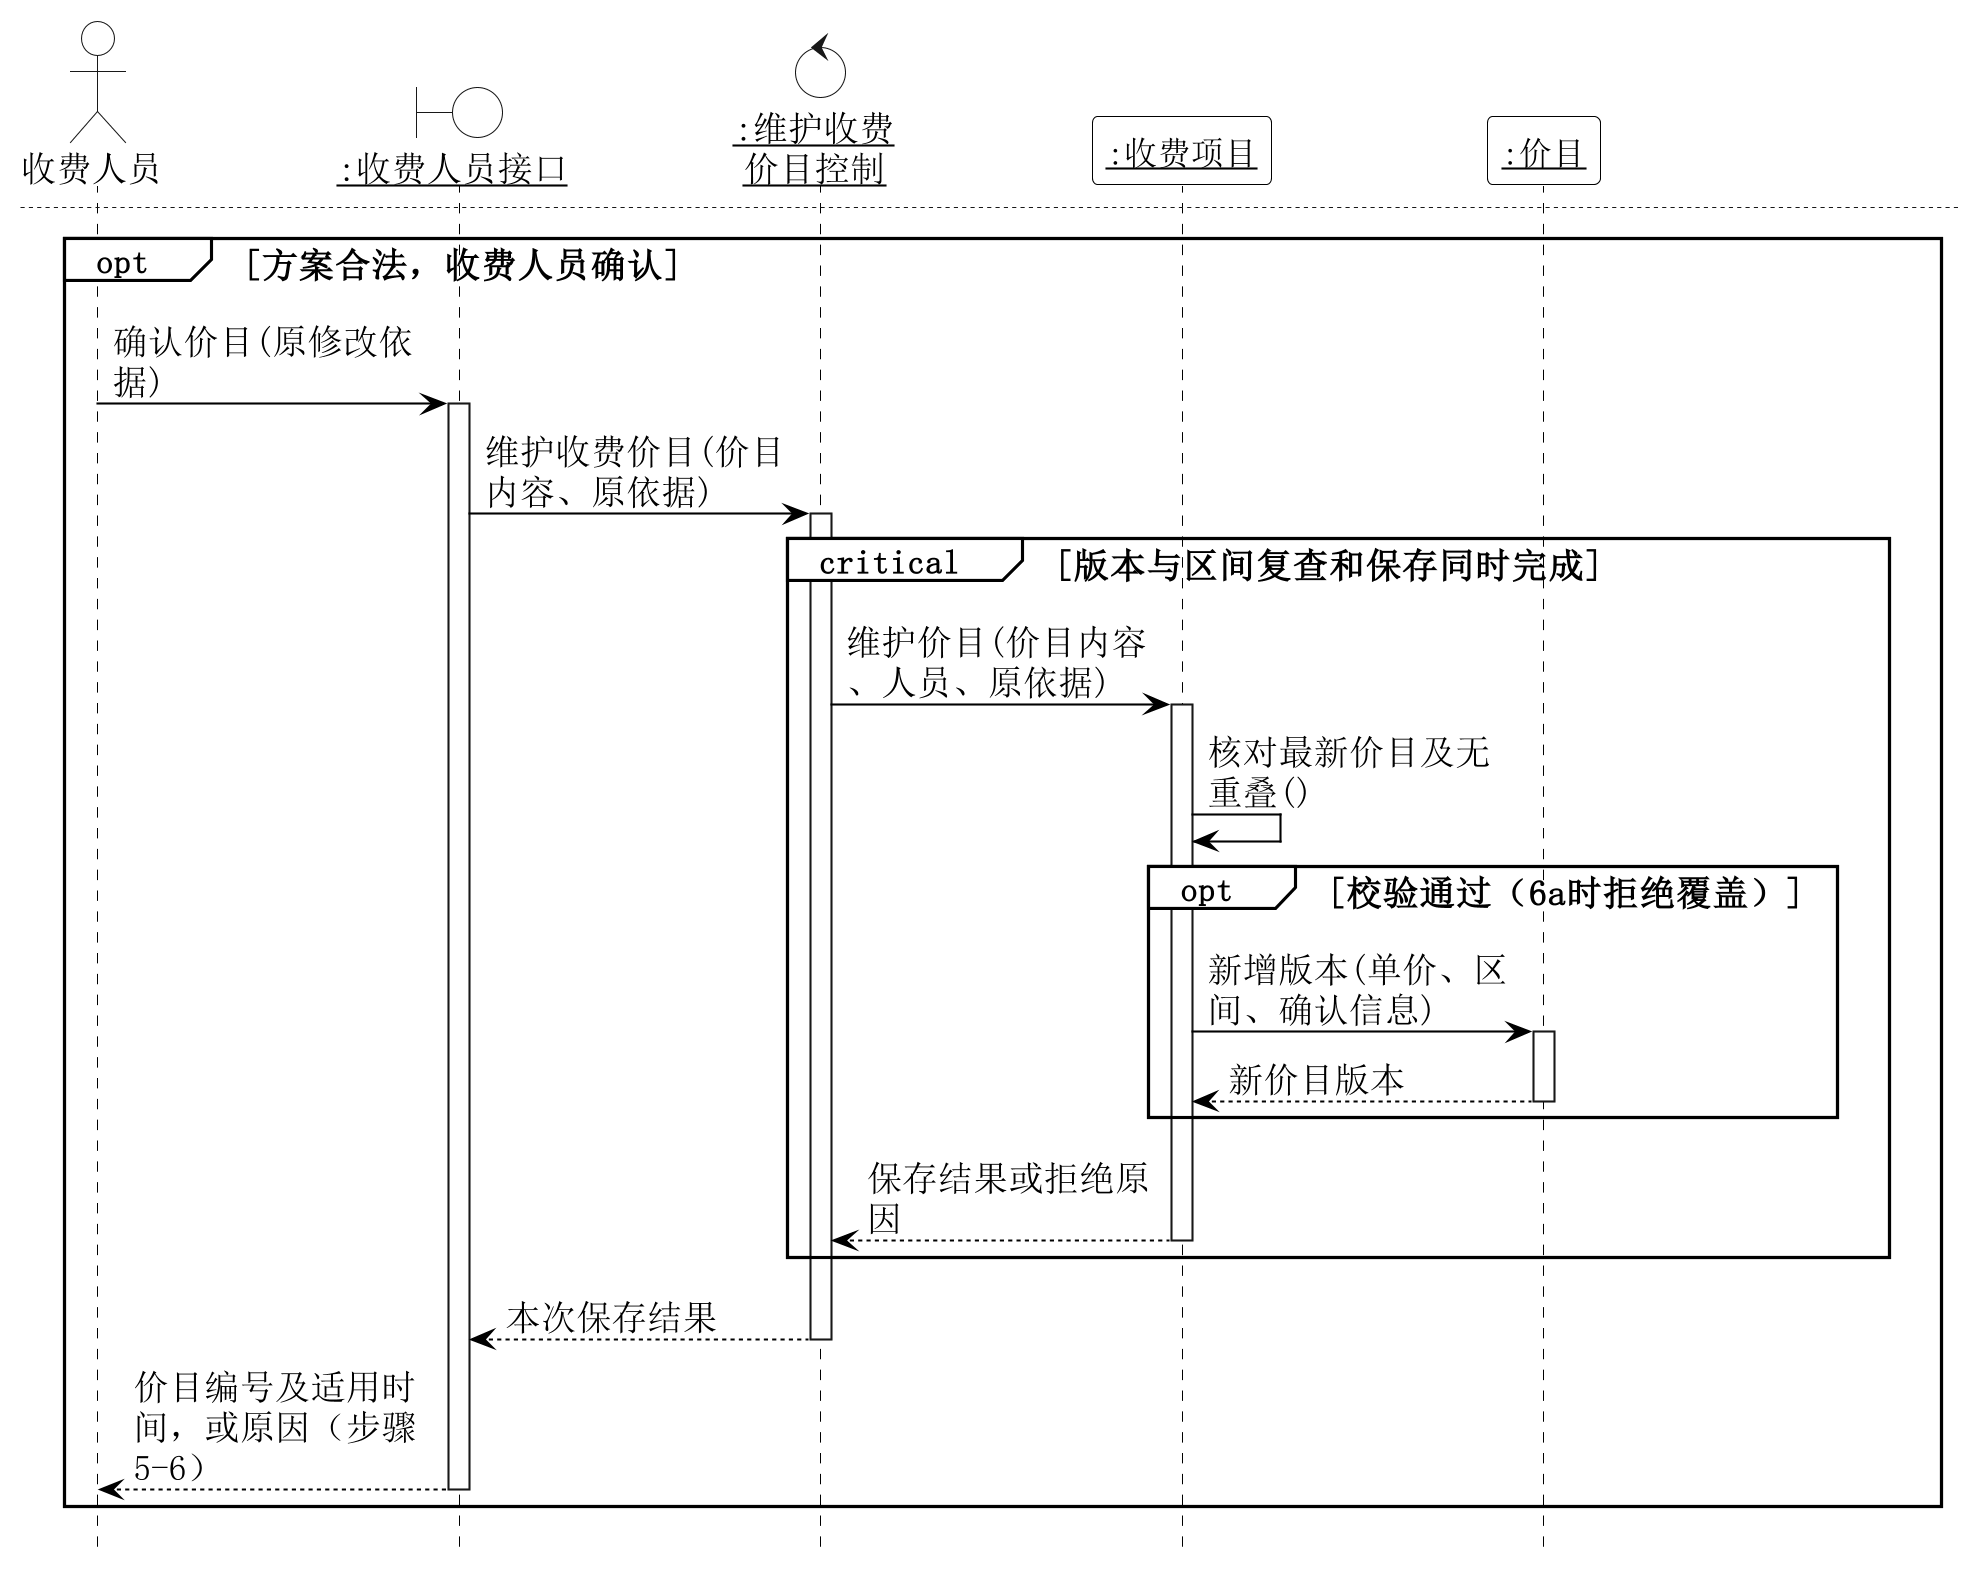
\includegraphics[width=\textwidth,height=21.3cm,keepaspectratio]{diagrams/13-05-analysis-sequence_001.png}
\par\vspace{0.5em}
{\normalsize 图\ref{fig:seq-05}（续）：UC-05 基本路径分析序列图}
\end{figure}

\clearpage
\noindent\textbf{UC-05 分析序列图：停止适用与价目区间衔接}
\medskip

图\ref{fig:seq-05-ext}对应扩展3a、4b，并沿用图\ref{fig:seq-05}的输入校验及6a版本检查。停止适用结束对应区间；衔接调整同时结束原区间并形成新价目。区间按开始包含、结束不包含解释，两个版本可在同一时点衔接；历史明细已关联的单价依据保留。

\begin{figure}[!htbp]
\centering
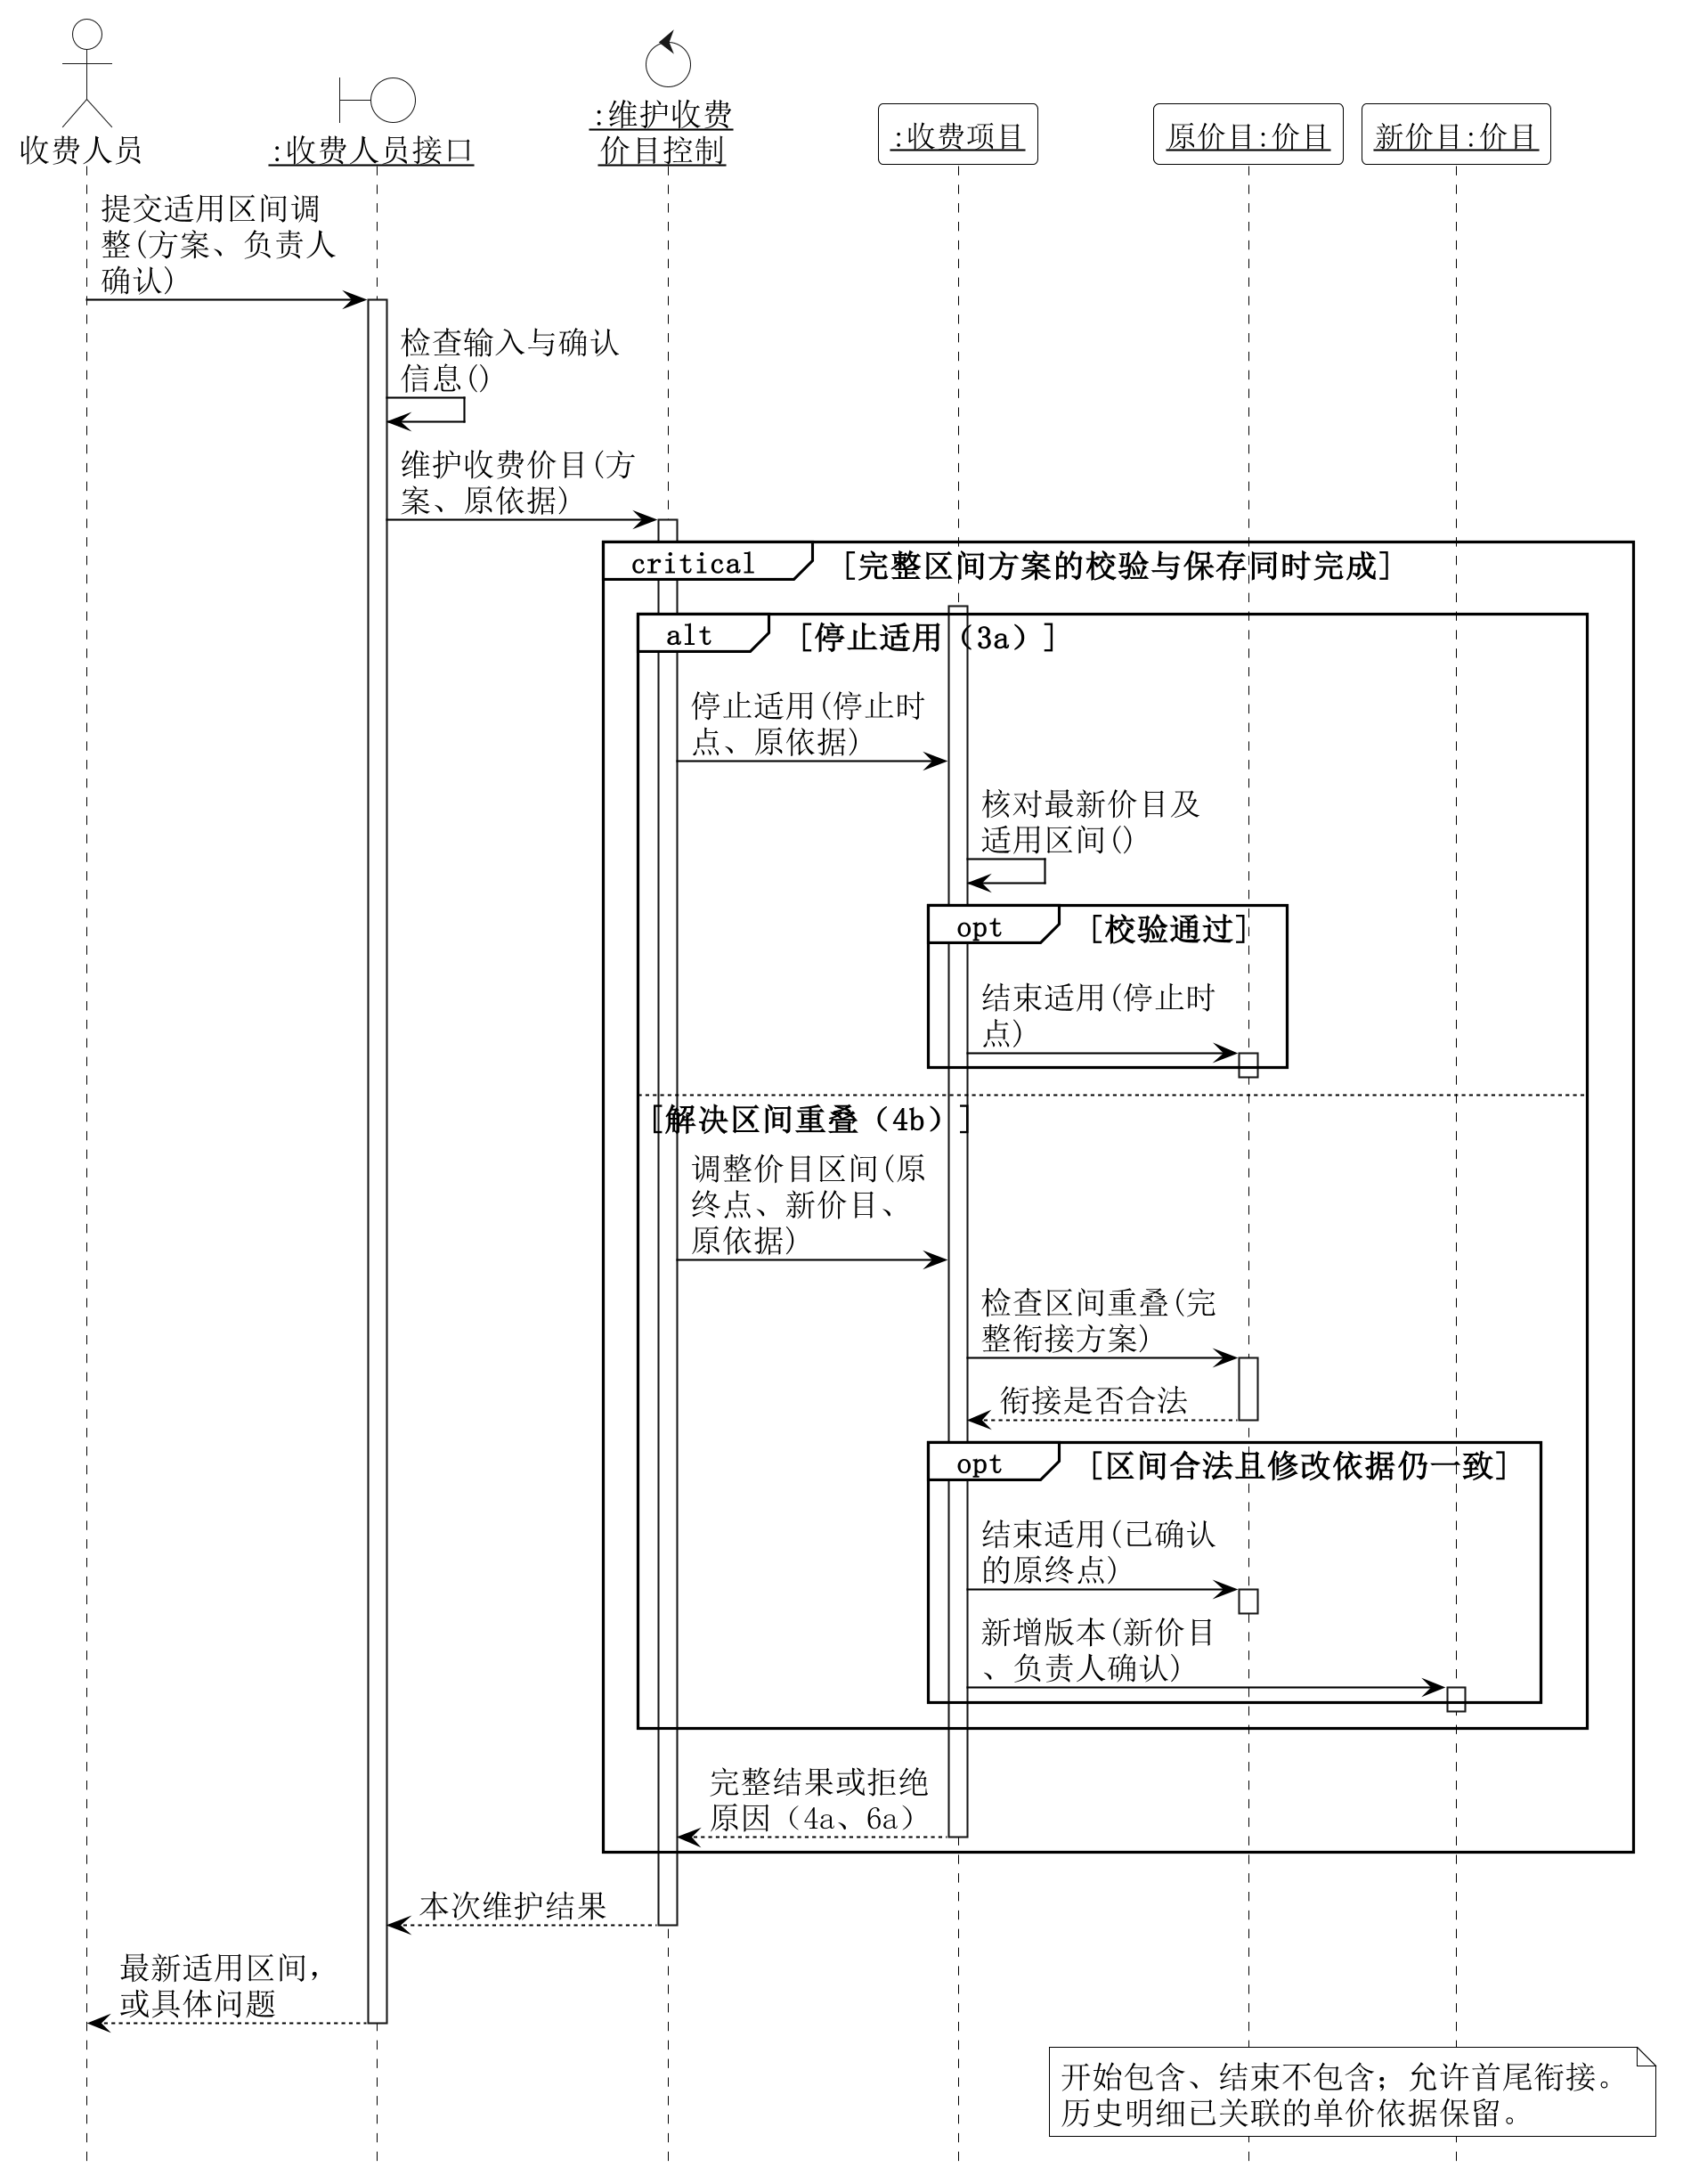
\includegraphics[width=\textwidth,height=20.4cm,keepaspectratio]{diagrams/13-05a-analysis-sequence.png}
\caption{UC-05 停止适用与价目区间衔接分析序列图}
\label{fig:seq-05-ext}
\end{figure}

\clearpage
\subsubsection{UC-06：查询待结算费用}
\medskip

图\ref{fig:seq-06}对应费用查询的基本路径，并合并未确认、缺价及已结清等简单扩展。就诊提供当前诊疗确认，诊疗确认组织计费判断并汇总费用，诊疗明细按已关联价目计算金额。控制类负责组织步骤，不计算金额。

\begin{figure}[!htbp]
\centering
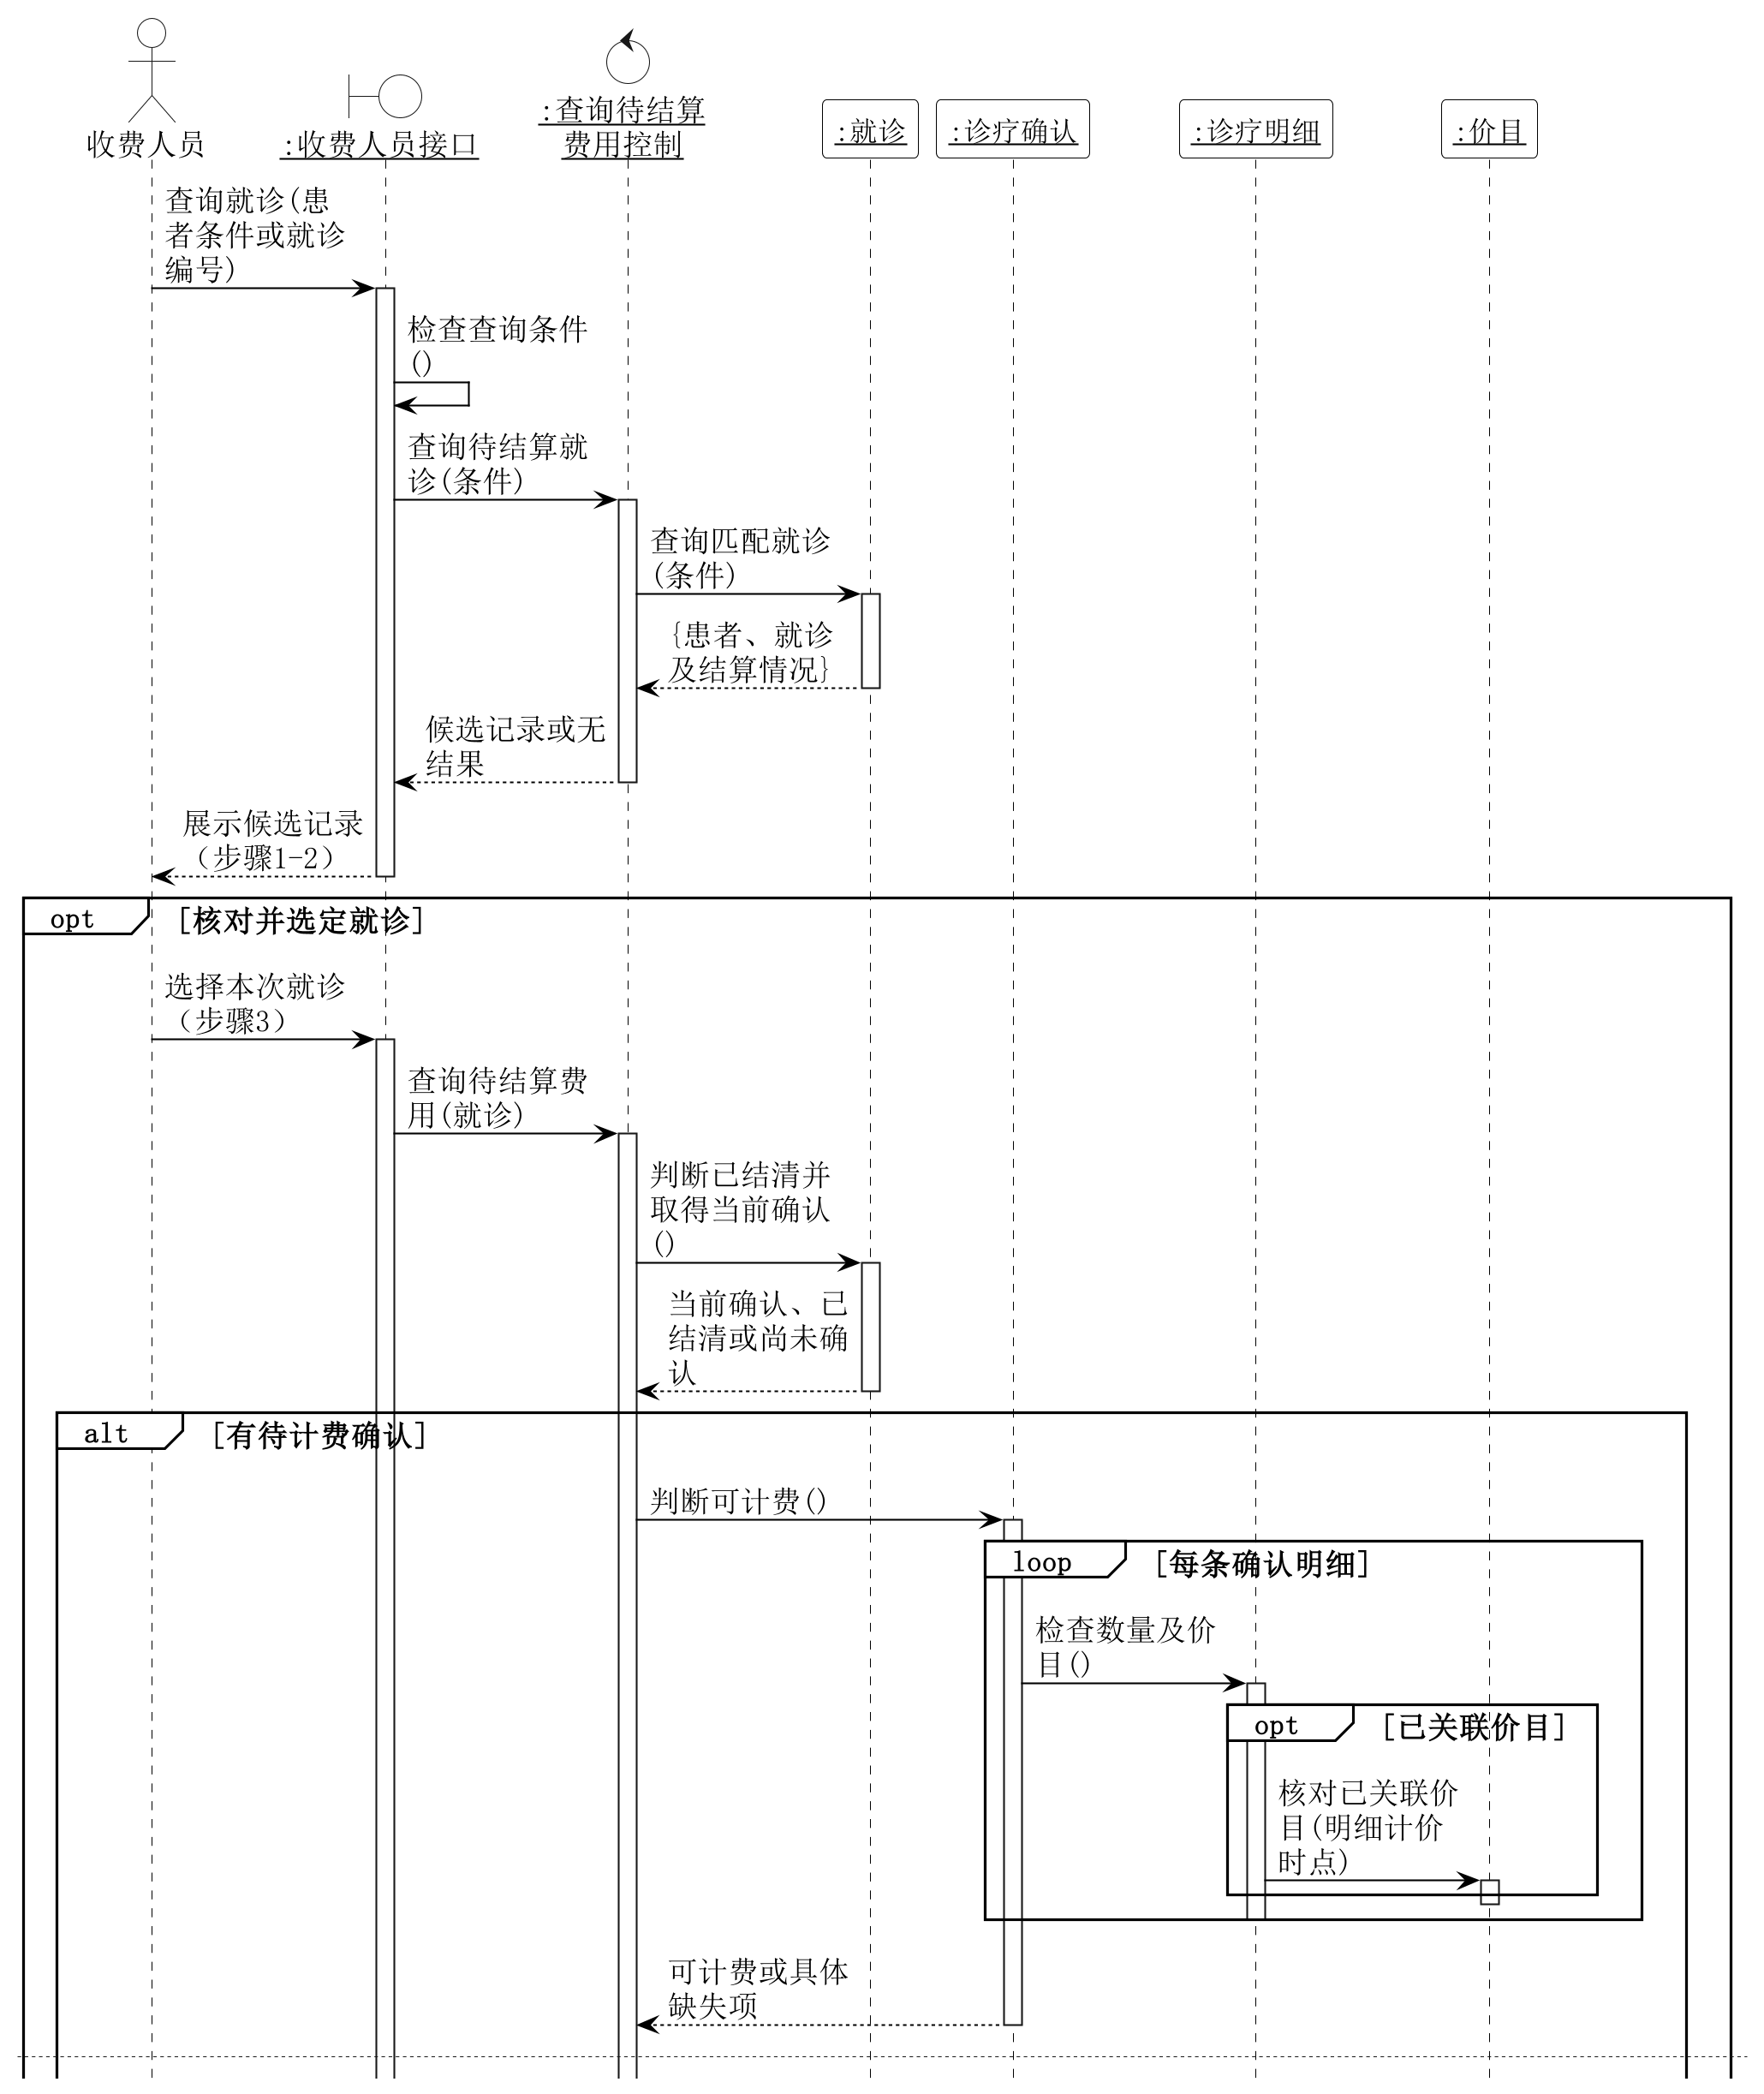
\includegraphics[width=\textwidth,height=20.4cm,keepaspectratio]{diagrams/13-06-analysis-sequence.png}
\caption{UC-06 基本路径分析序列图}
\label{fig:seq-06}
\end{figure}
\clearpage
\noindent\textbf{UC-06 分析序列图：基本路径（续）}
\medskip

\begin{figure}[!htbp]
\centering
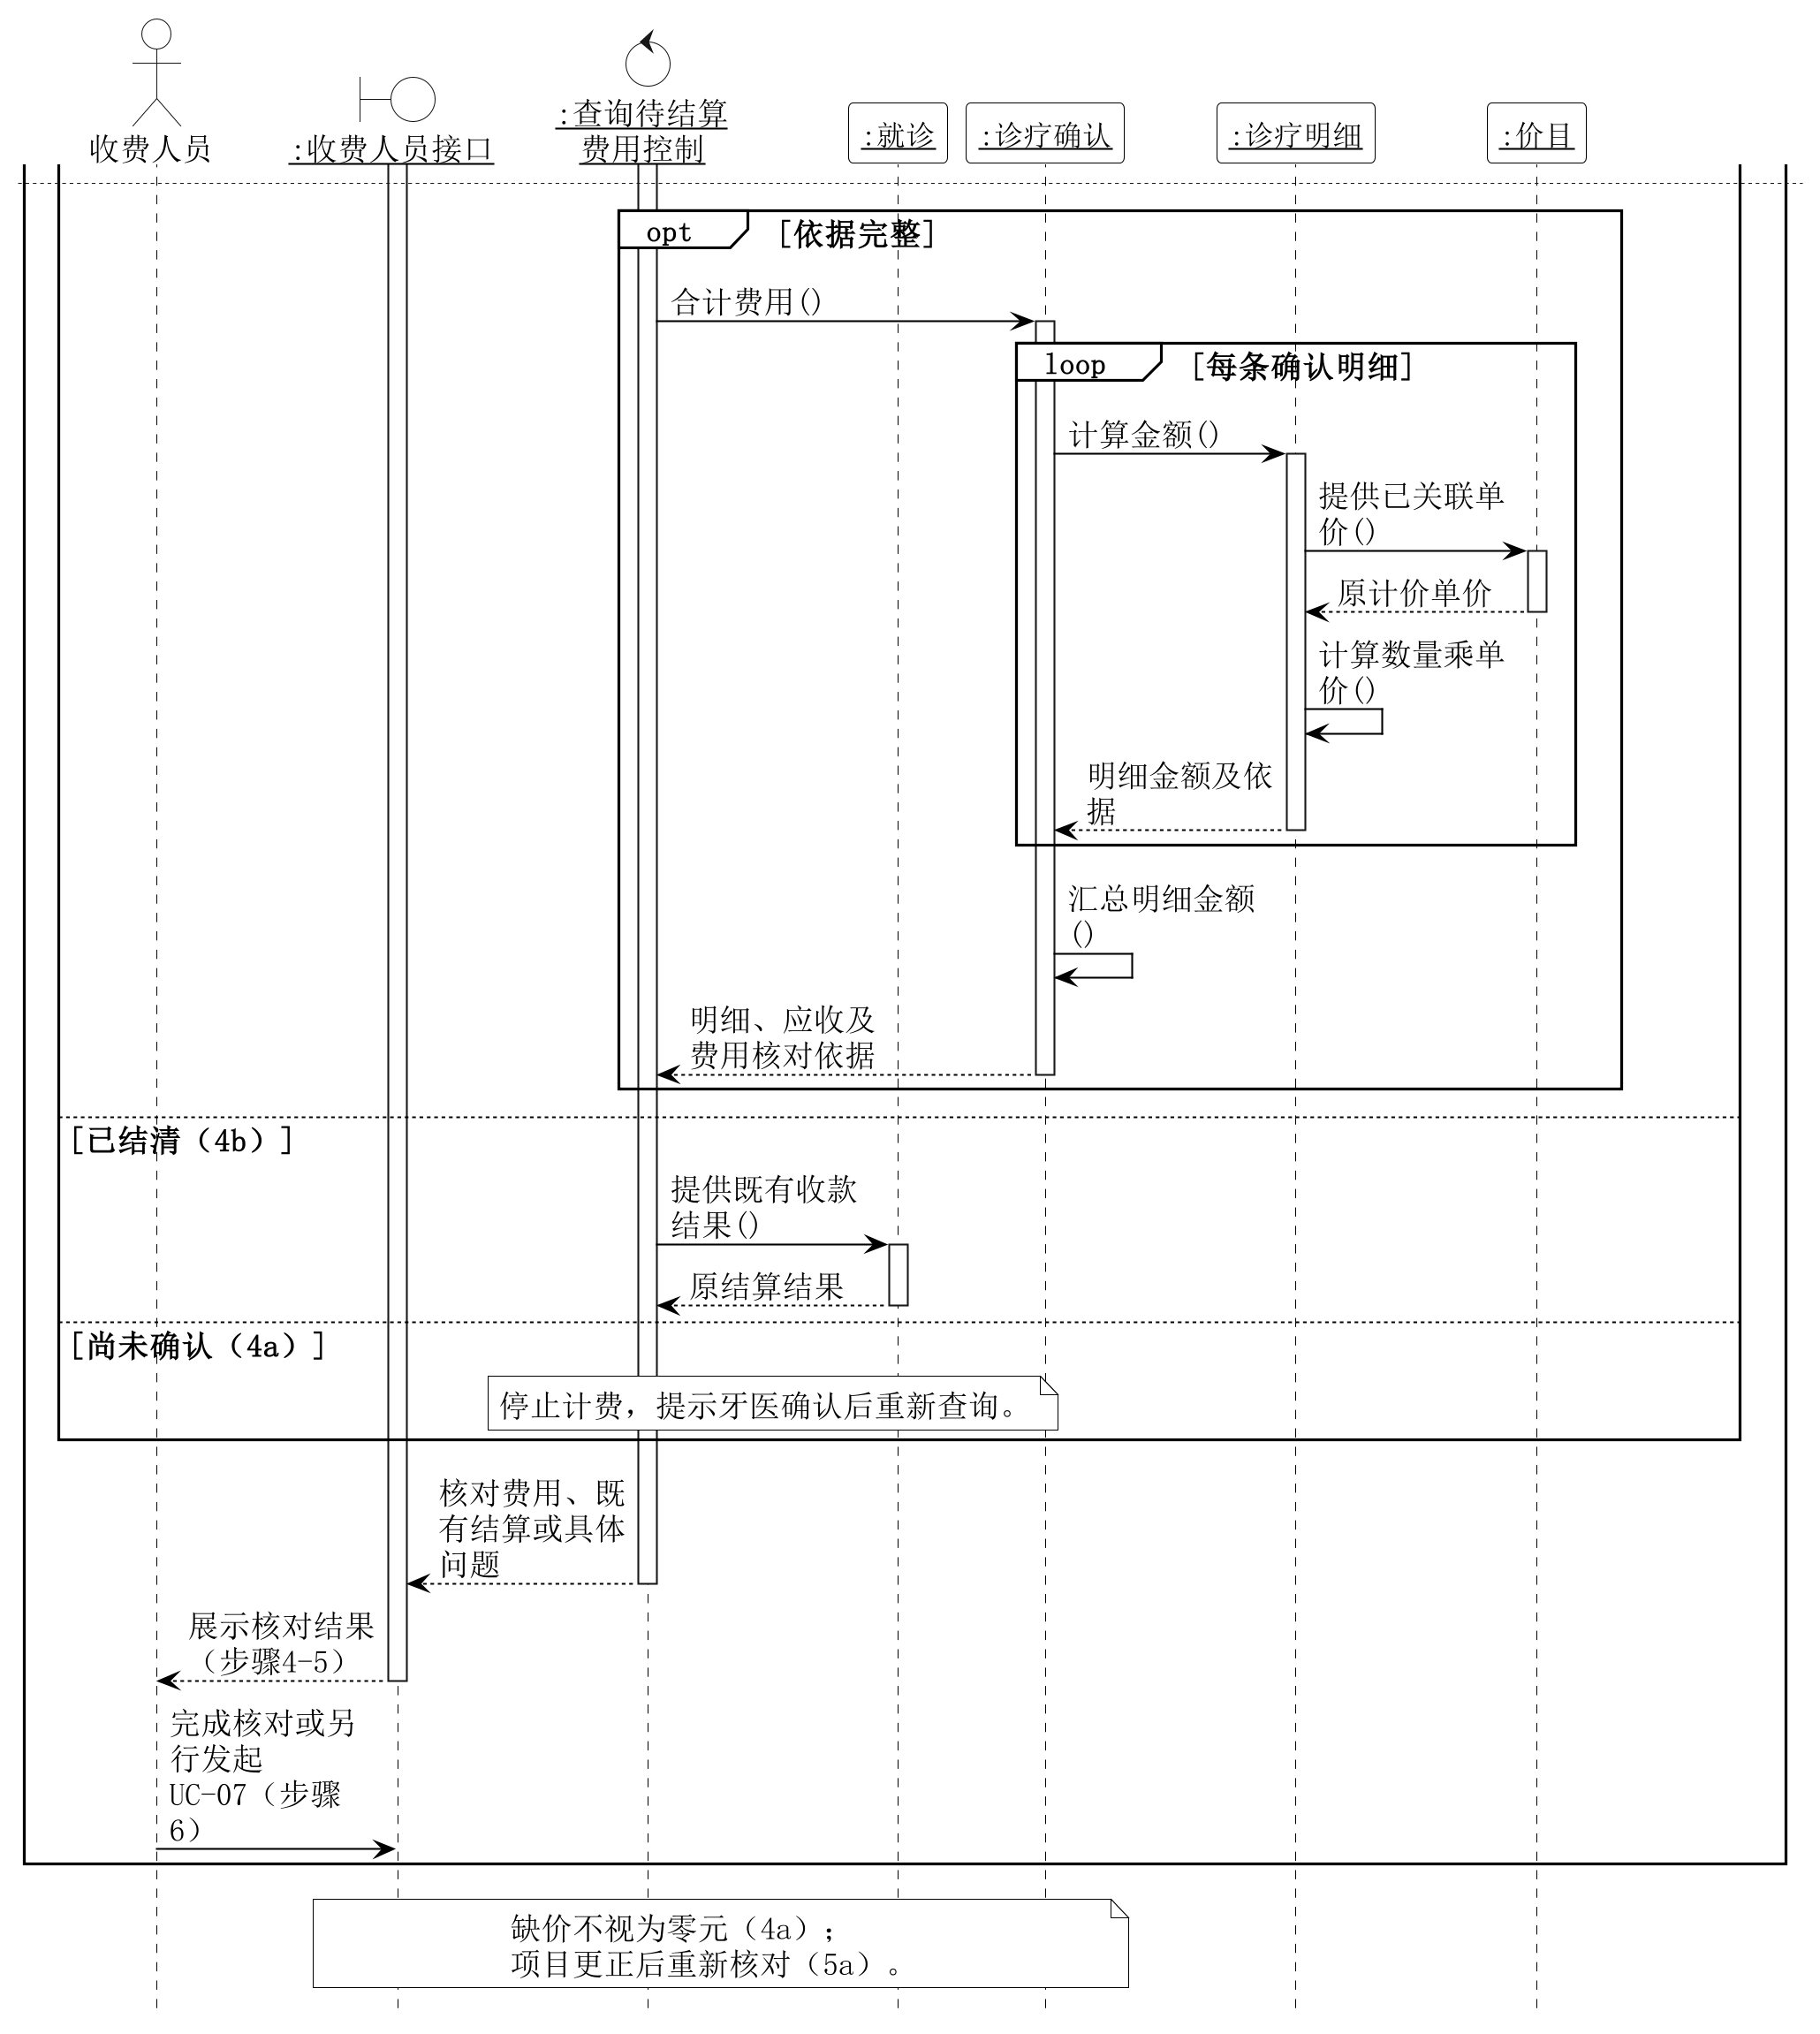
\includegraphics[width=\textwidth,height=21.3cm,keepaspectratio]{diagrams/13-06-analysis-sequence_001.png}
\par\vspace{0.5em}
{\normalsize 图\ref{fig:seq-06}（续）：UC-06 基本路径分析序列图}
\end{figure}

\clearpage
\subsubsection{UC-07：登记现金收款}
\medskip

图\ref{fig:seq-07}对应现金收款的基本路径。就诊核验结算条件，诊疗确认核验费用依据，现金收款检查实收、计算找零与净收。保存时再次检查当前依据，收款与结清同时生效；收据来自已经保存的收款。

\begin{figure}[!htbp]
\centering
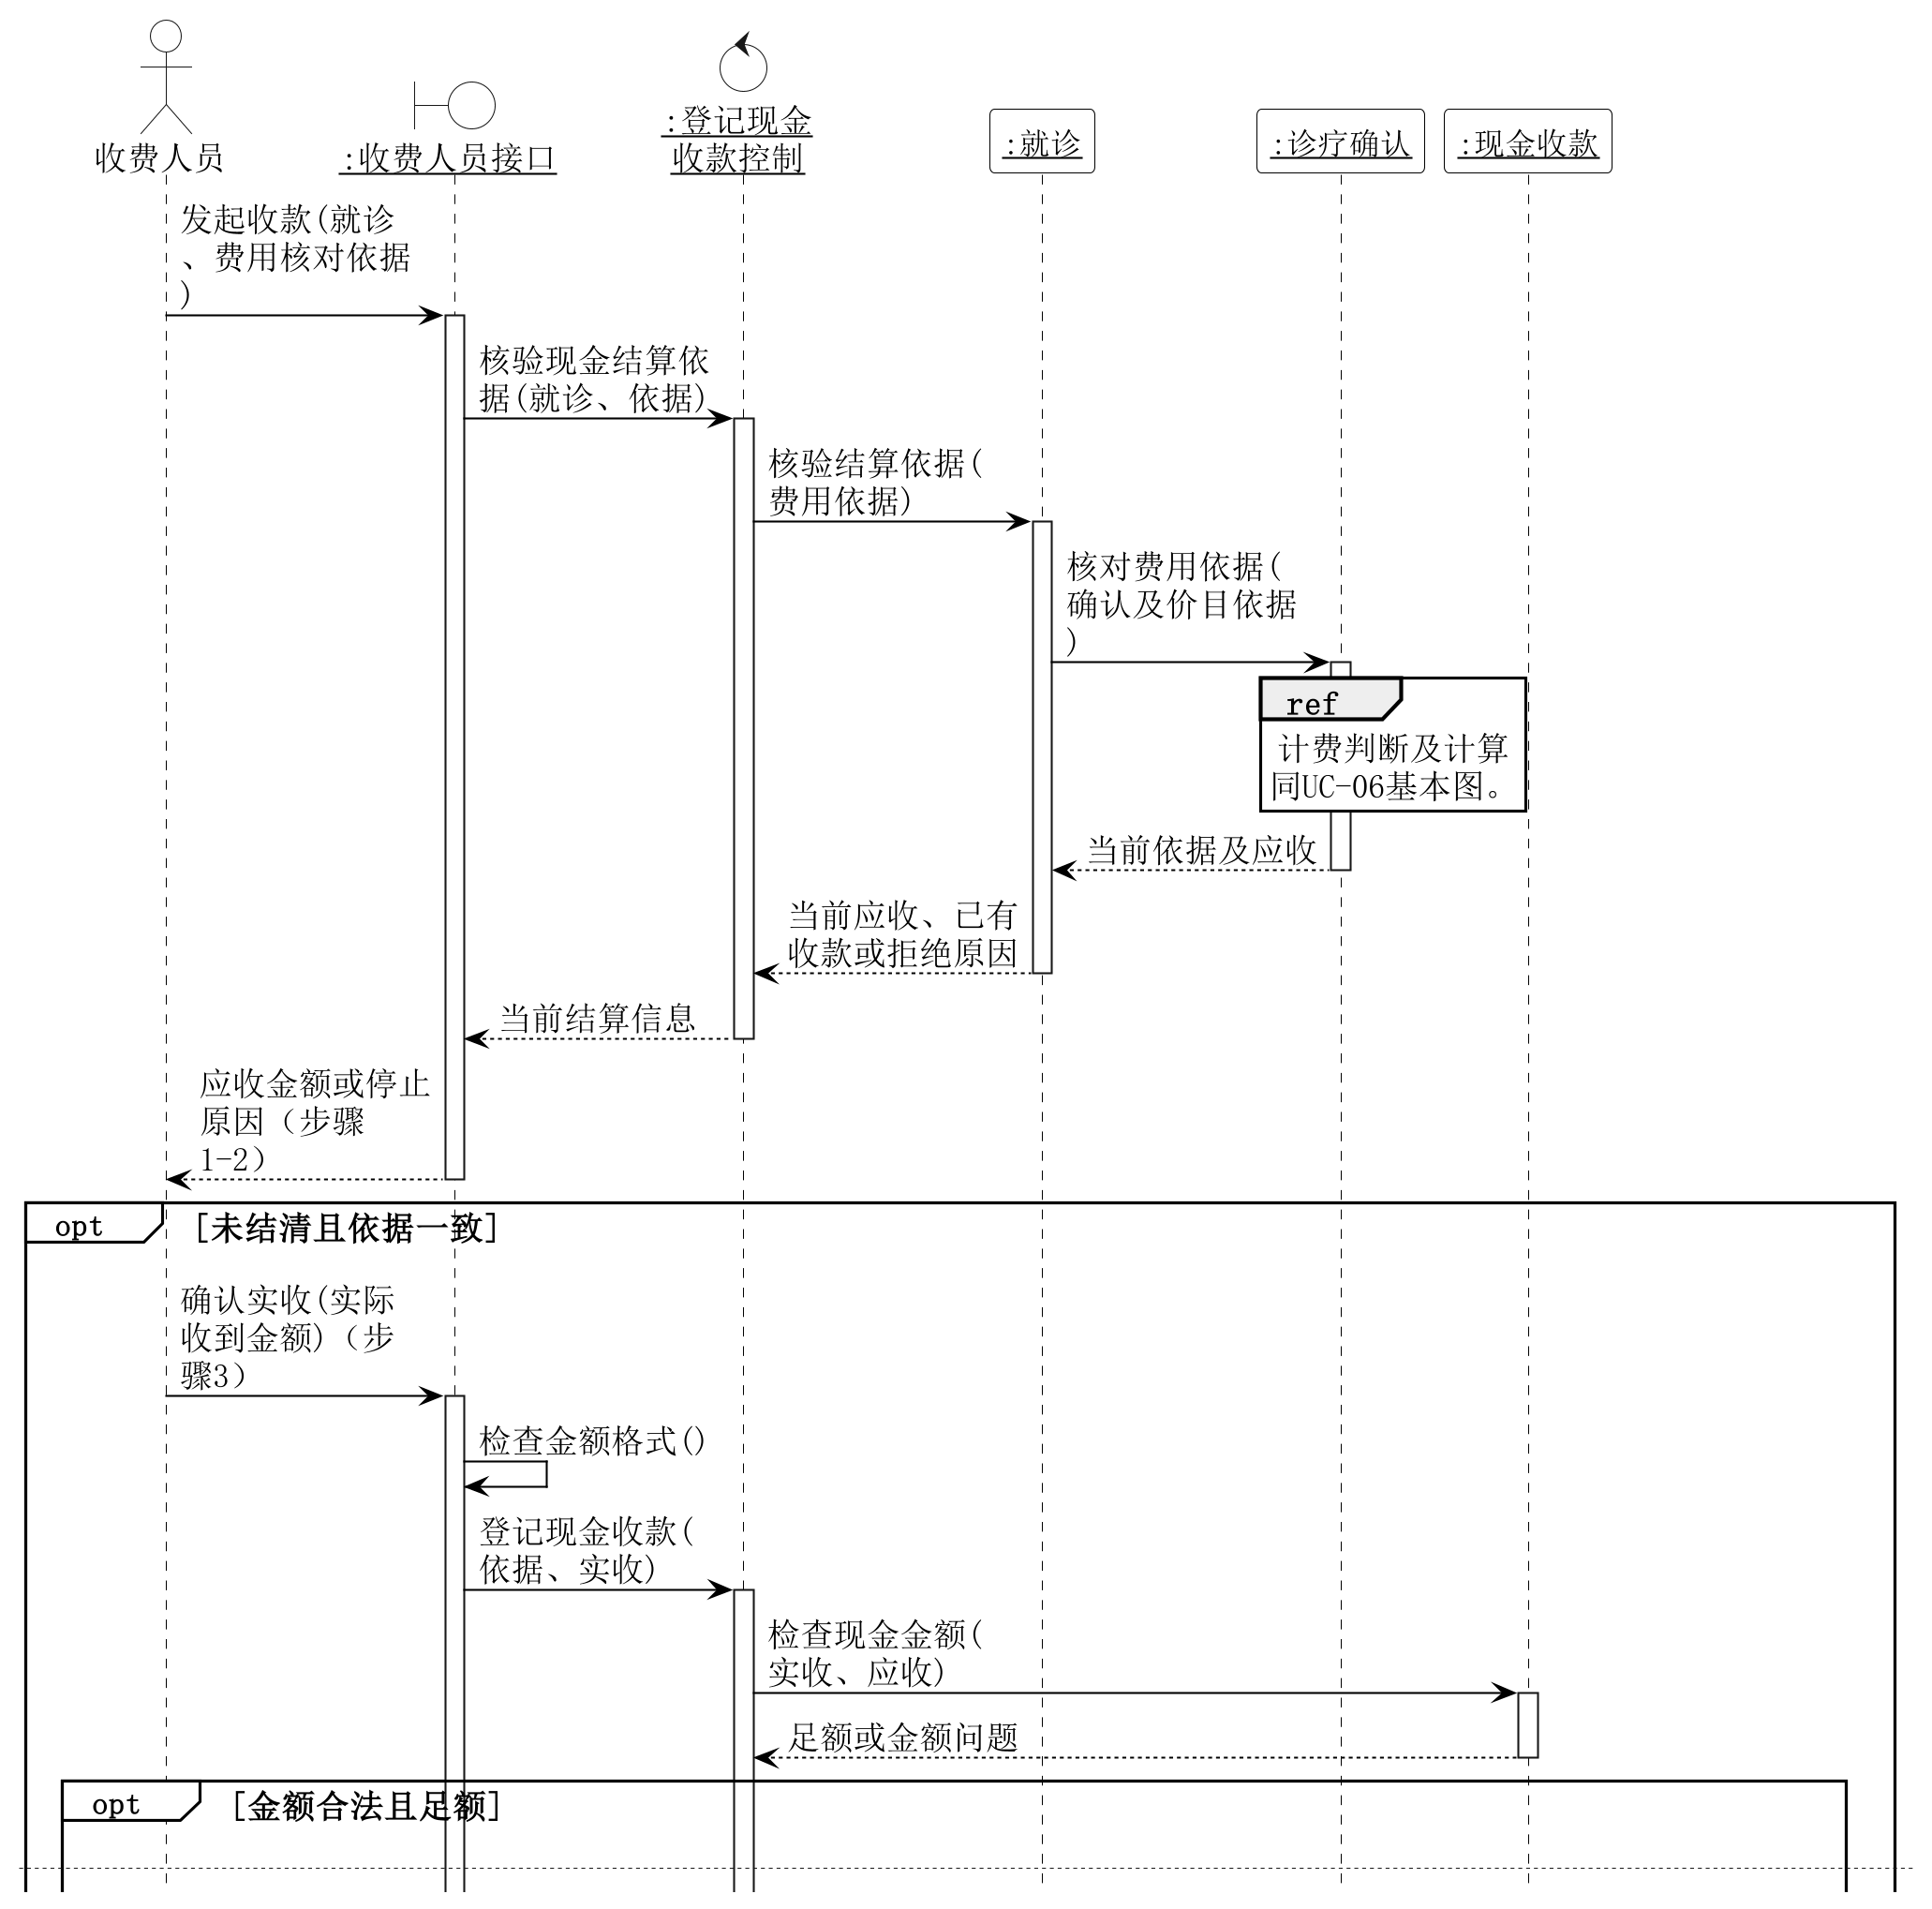
\includegraphics[width=\textwidth,height=20.4cm,keepaspectratio]{diagrams/13-07-analysis-sequence.png}
\caption{UC-07 基本路径分析序列图（扩展见图\ref{fig:seq-07-ext}）}
\label{fig:seq-07}
\end{figure}
\clearpage
\noindent\textbf{UC-07 分析序列图：基本路径（续）}
\medskip

\begin{figure}[!htbp]
\centering
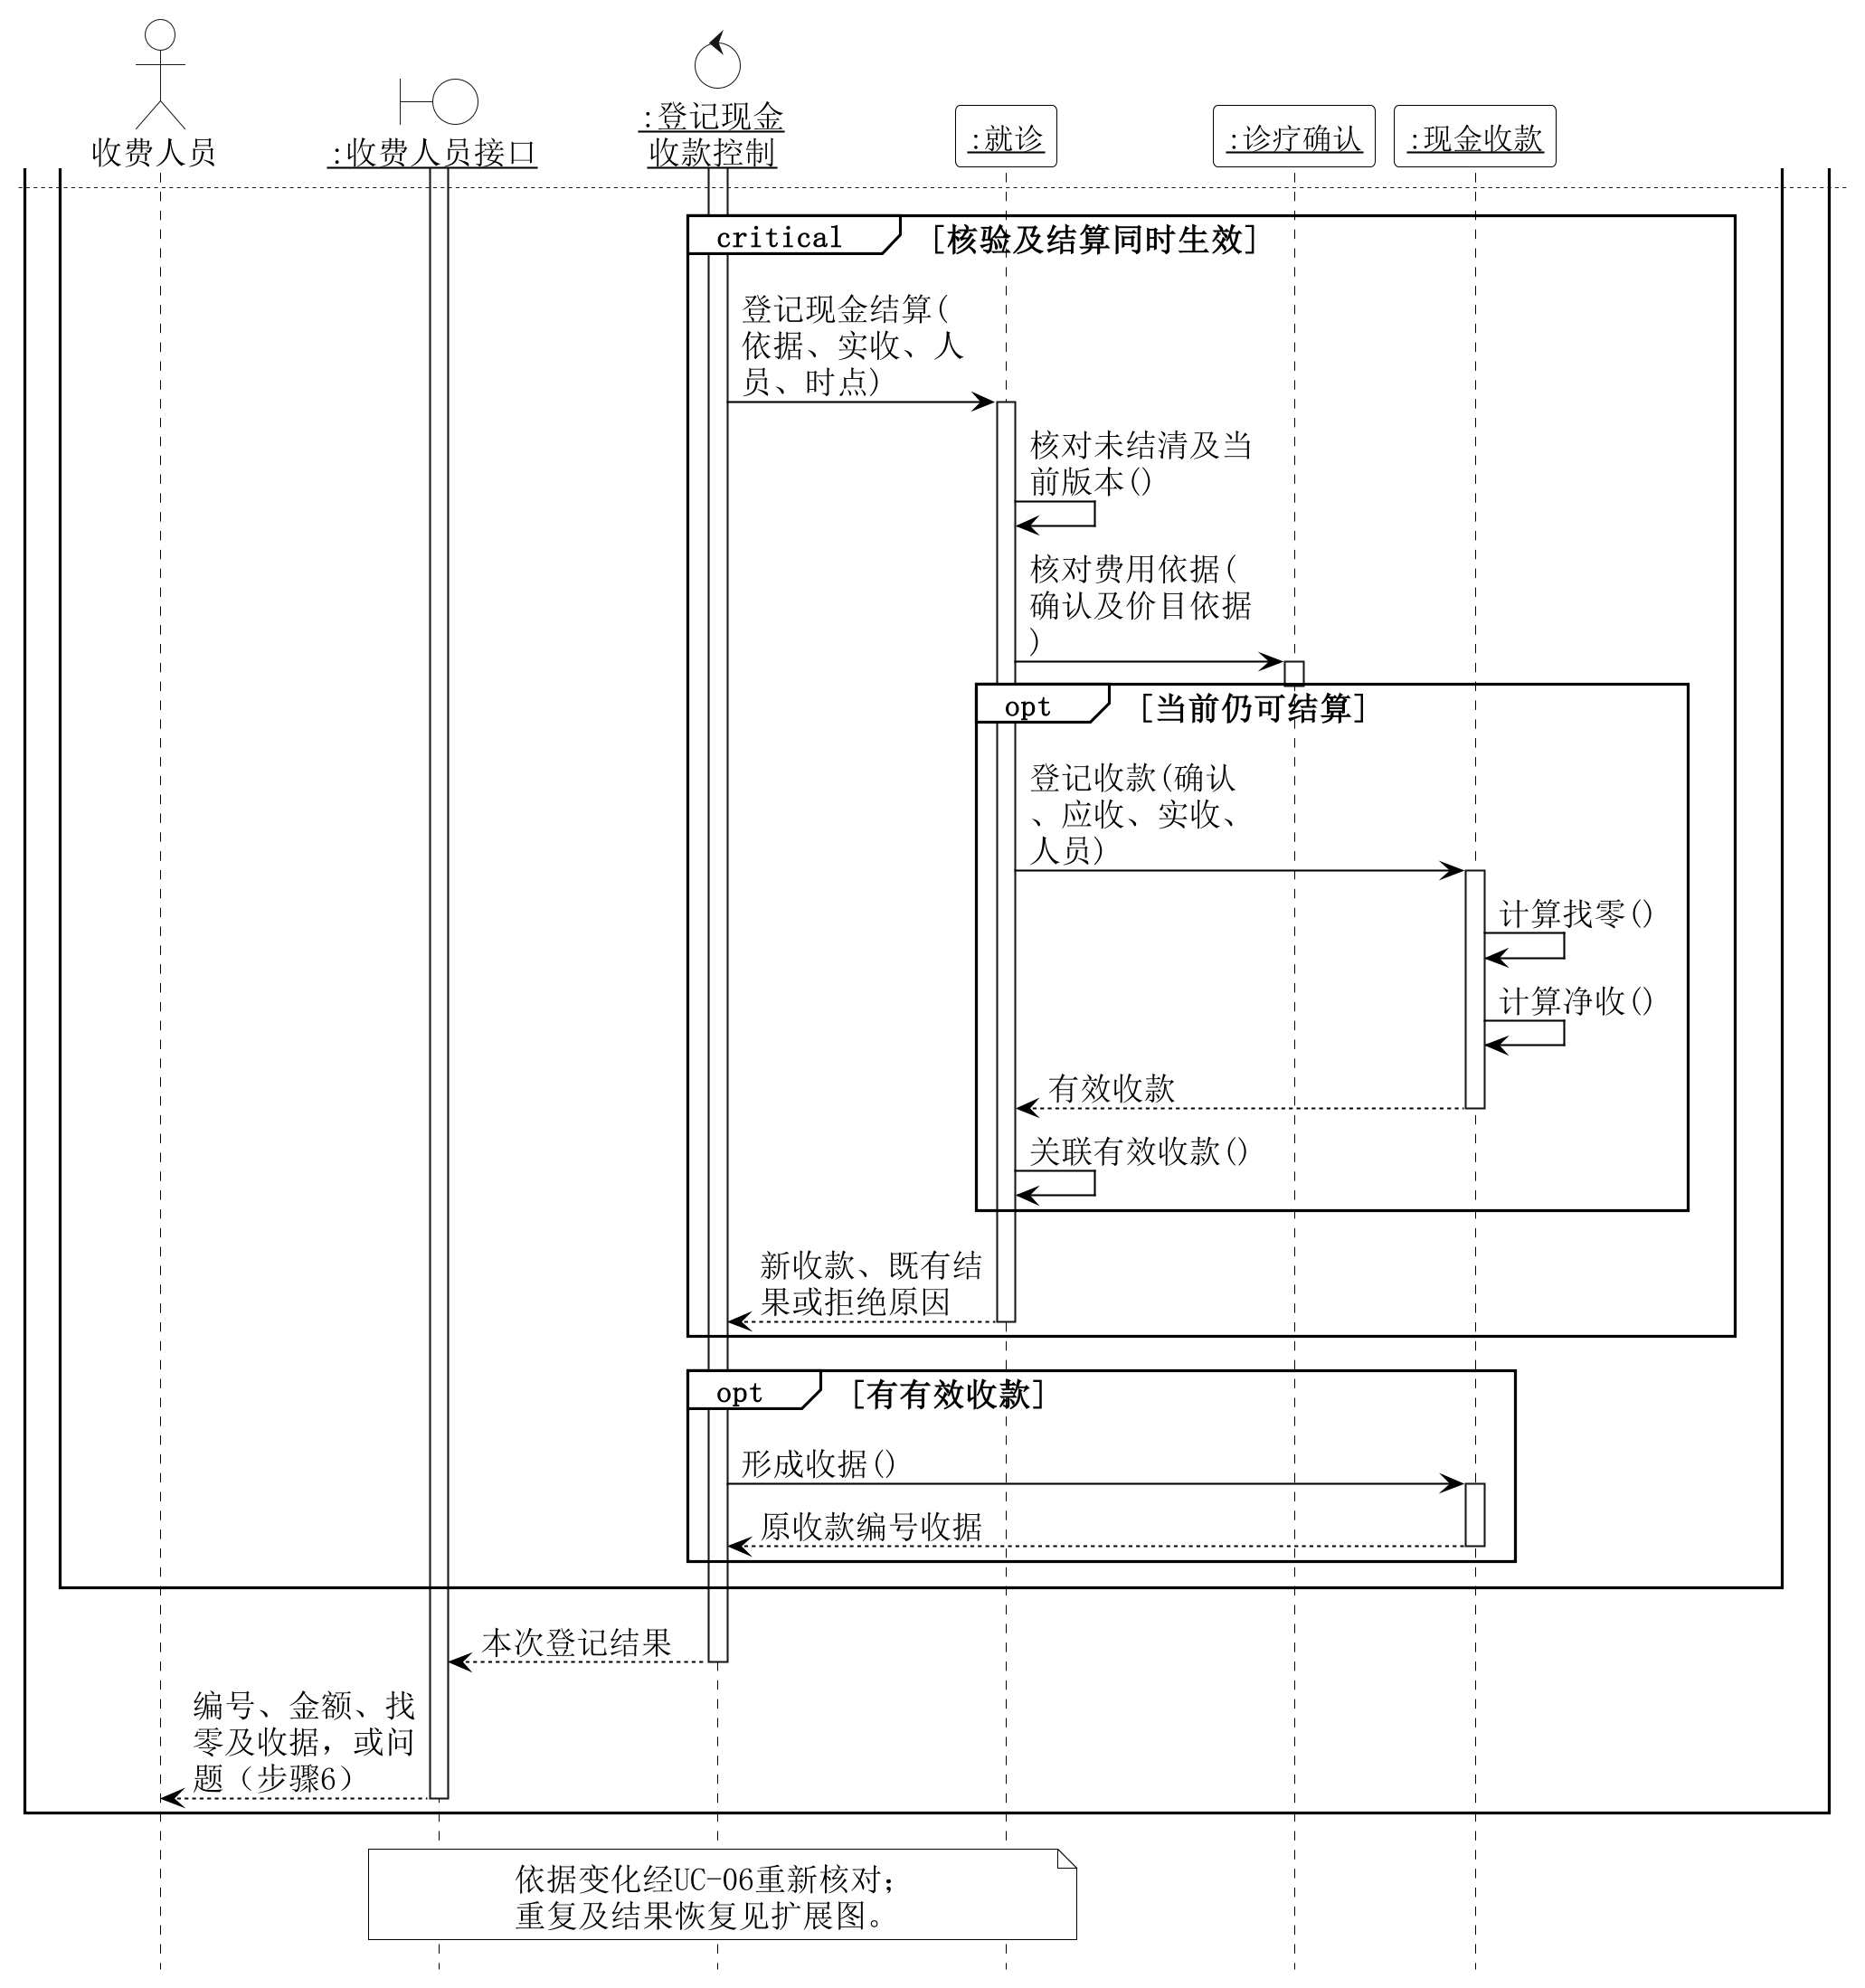
\includegraphics[width=\textwidth,height=21.3cm,keepaspectratio]{diagrams/13-07-analysis-sequence_001.png}
\par\vspace{0.5em}
{\normalsize 图\ref{fig:seq-07}（续）：UC-07 基本路径分析序列图}
\end{figure}

\clearpage
\noindent\textbf{UC-07 分析序列图：重复提交与收款结果恢复}
\medskip

图\ref{fig:seq-07-ext}对应扩展4b、5a、6a。收到重复请求或未取得上次结果时，先查本次有效收款；已有收款则返回原编号及原金额，并重新形成收据。只有查询明确显示未结清且无有效收款、收费人员核实实际现金后，才按图\ref{fig:seq-07}重新校验并提交。

\begin{figure}[!htbp]
\centering
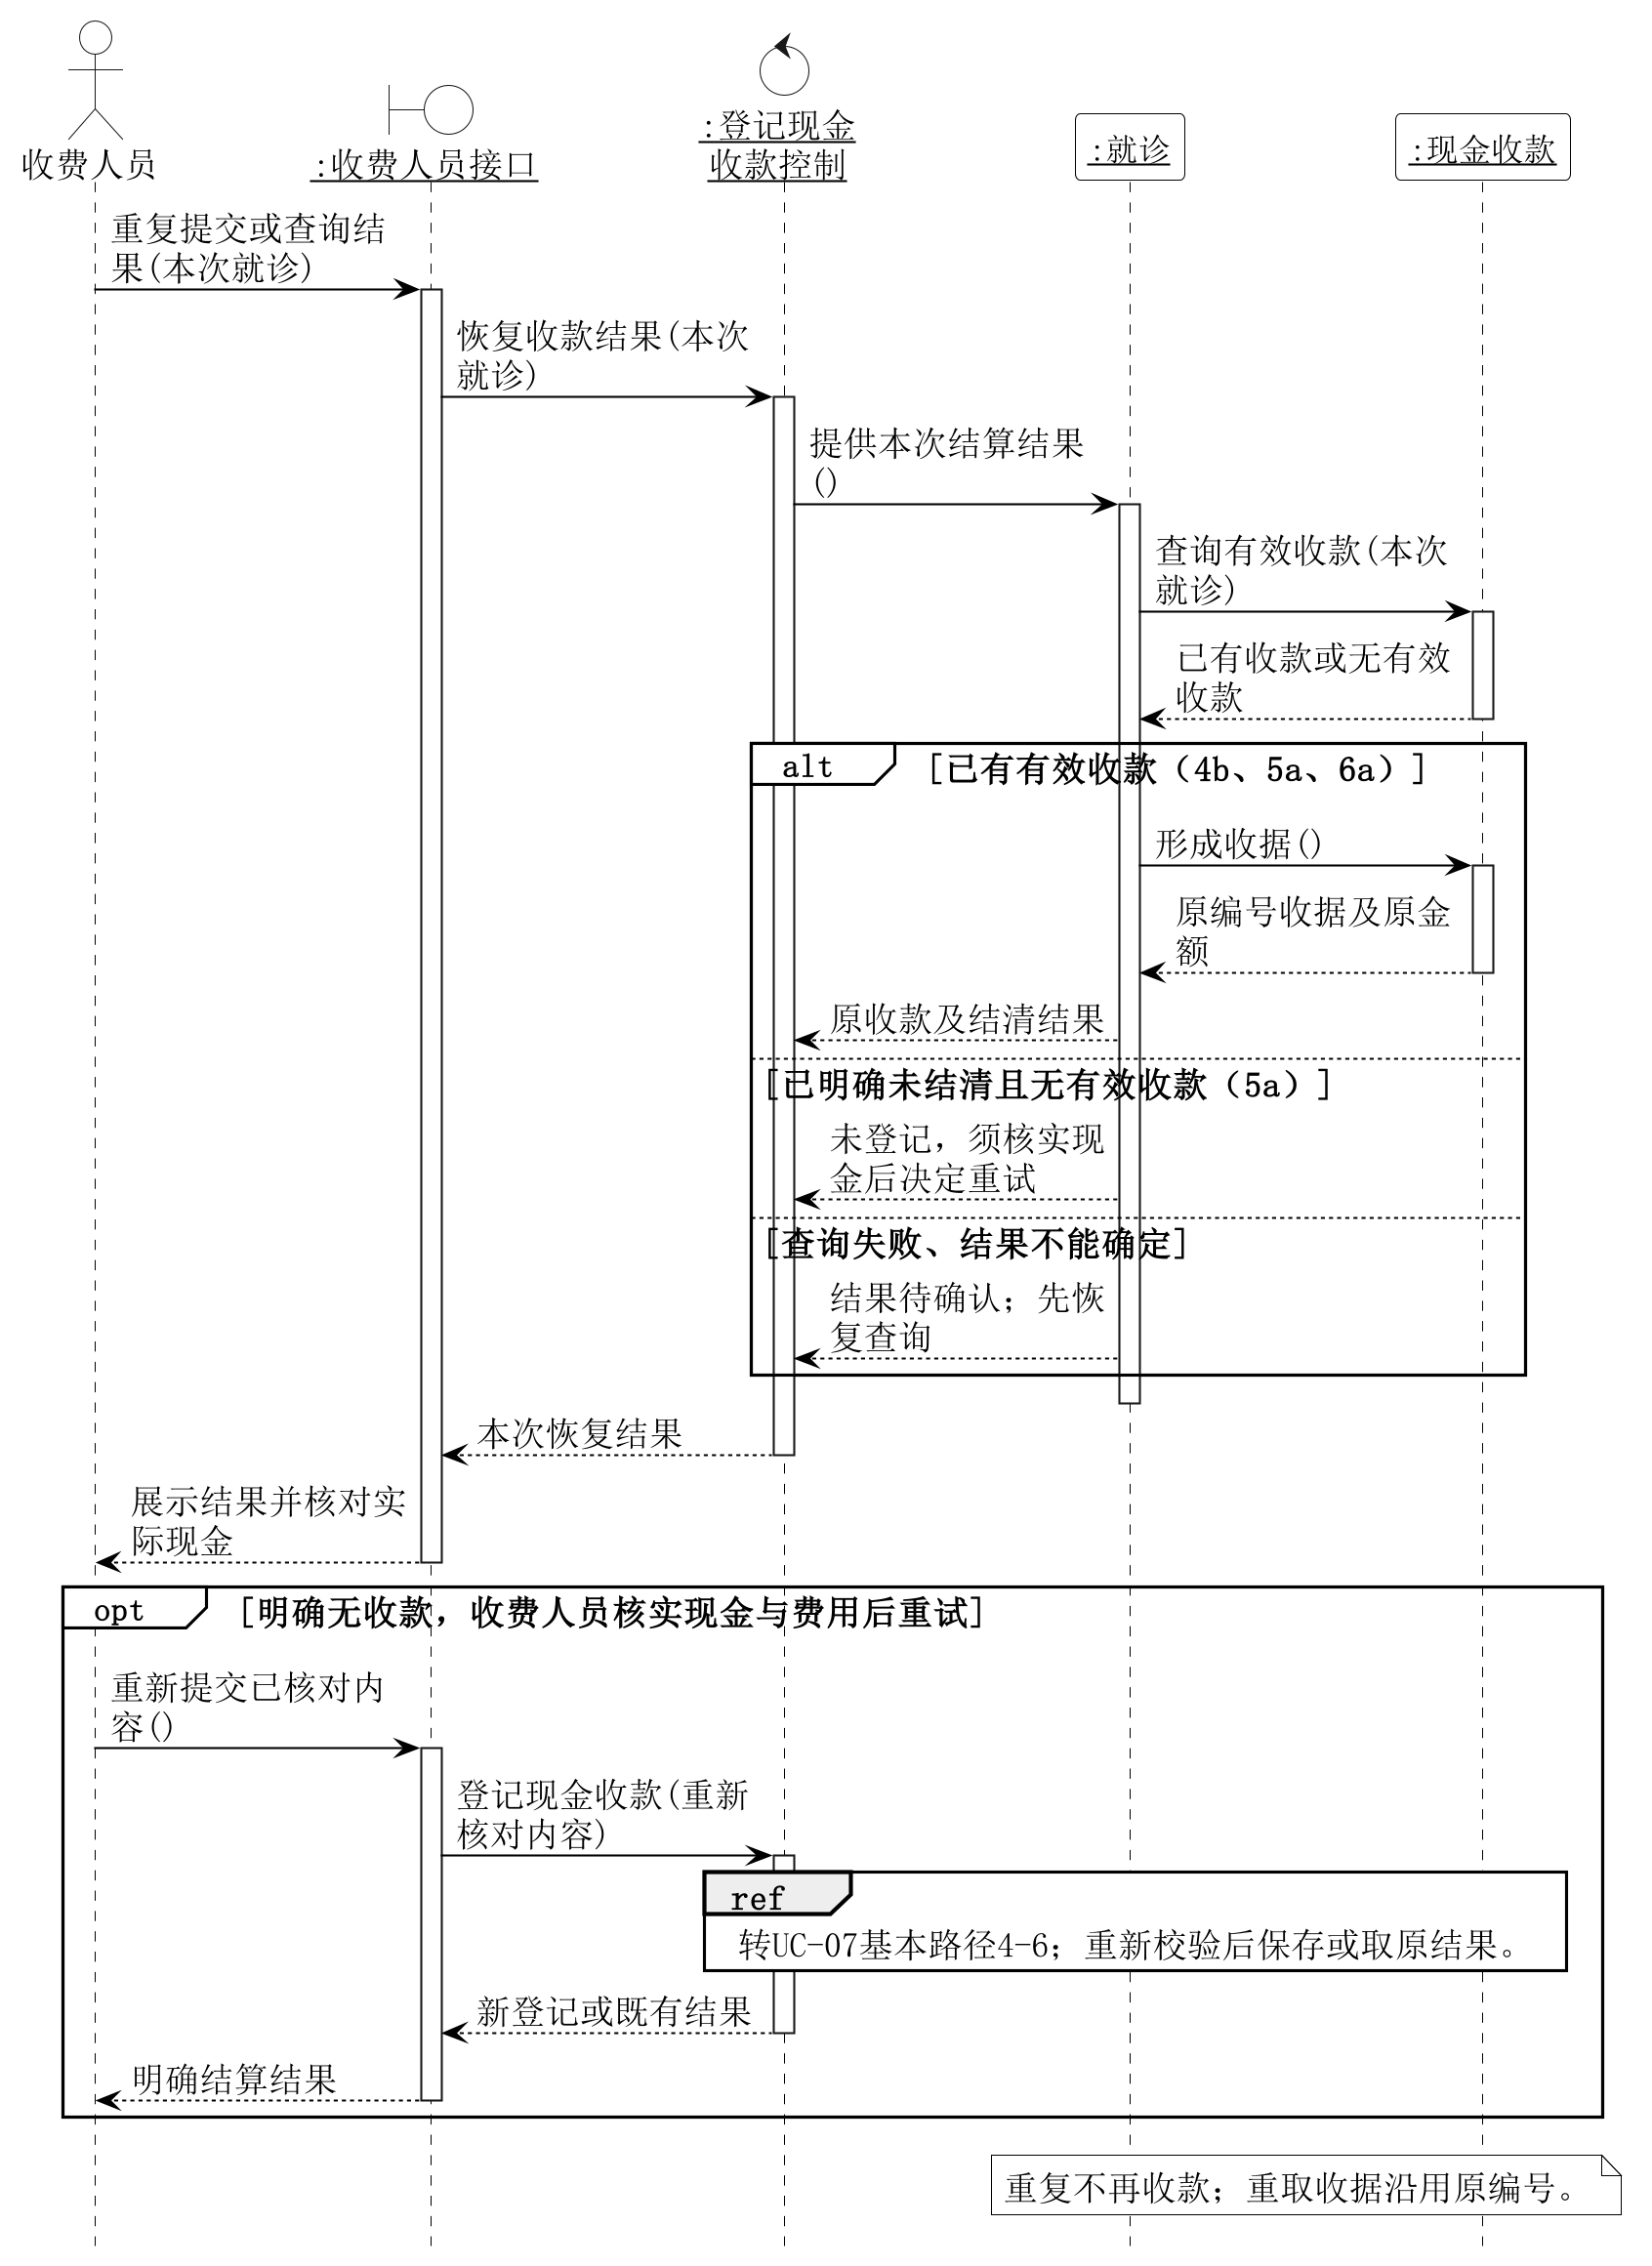
\includegraphics[width=\textwidth,height=20.4cm,keepaspectratio]{diagrams/13-07a-analysis-sequence.png}
\caption{UC-07 重复提交与收款结果恢复分析序列图}
\label{fig:seq-07-ext}
\end{figure}

\clearpage
\clearpage
\subsubsection{UC-08：维护患者资料}

本图按规约分配患者、患者资料变更、职员的业务责任。
\begin{figure}[!htbp]
\centering
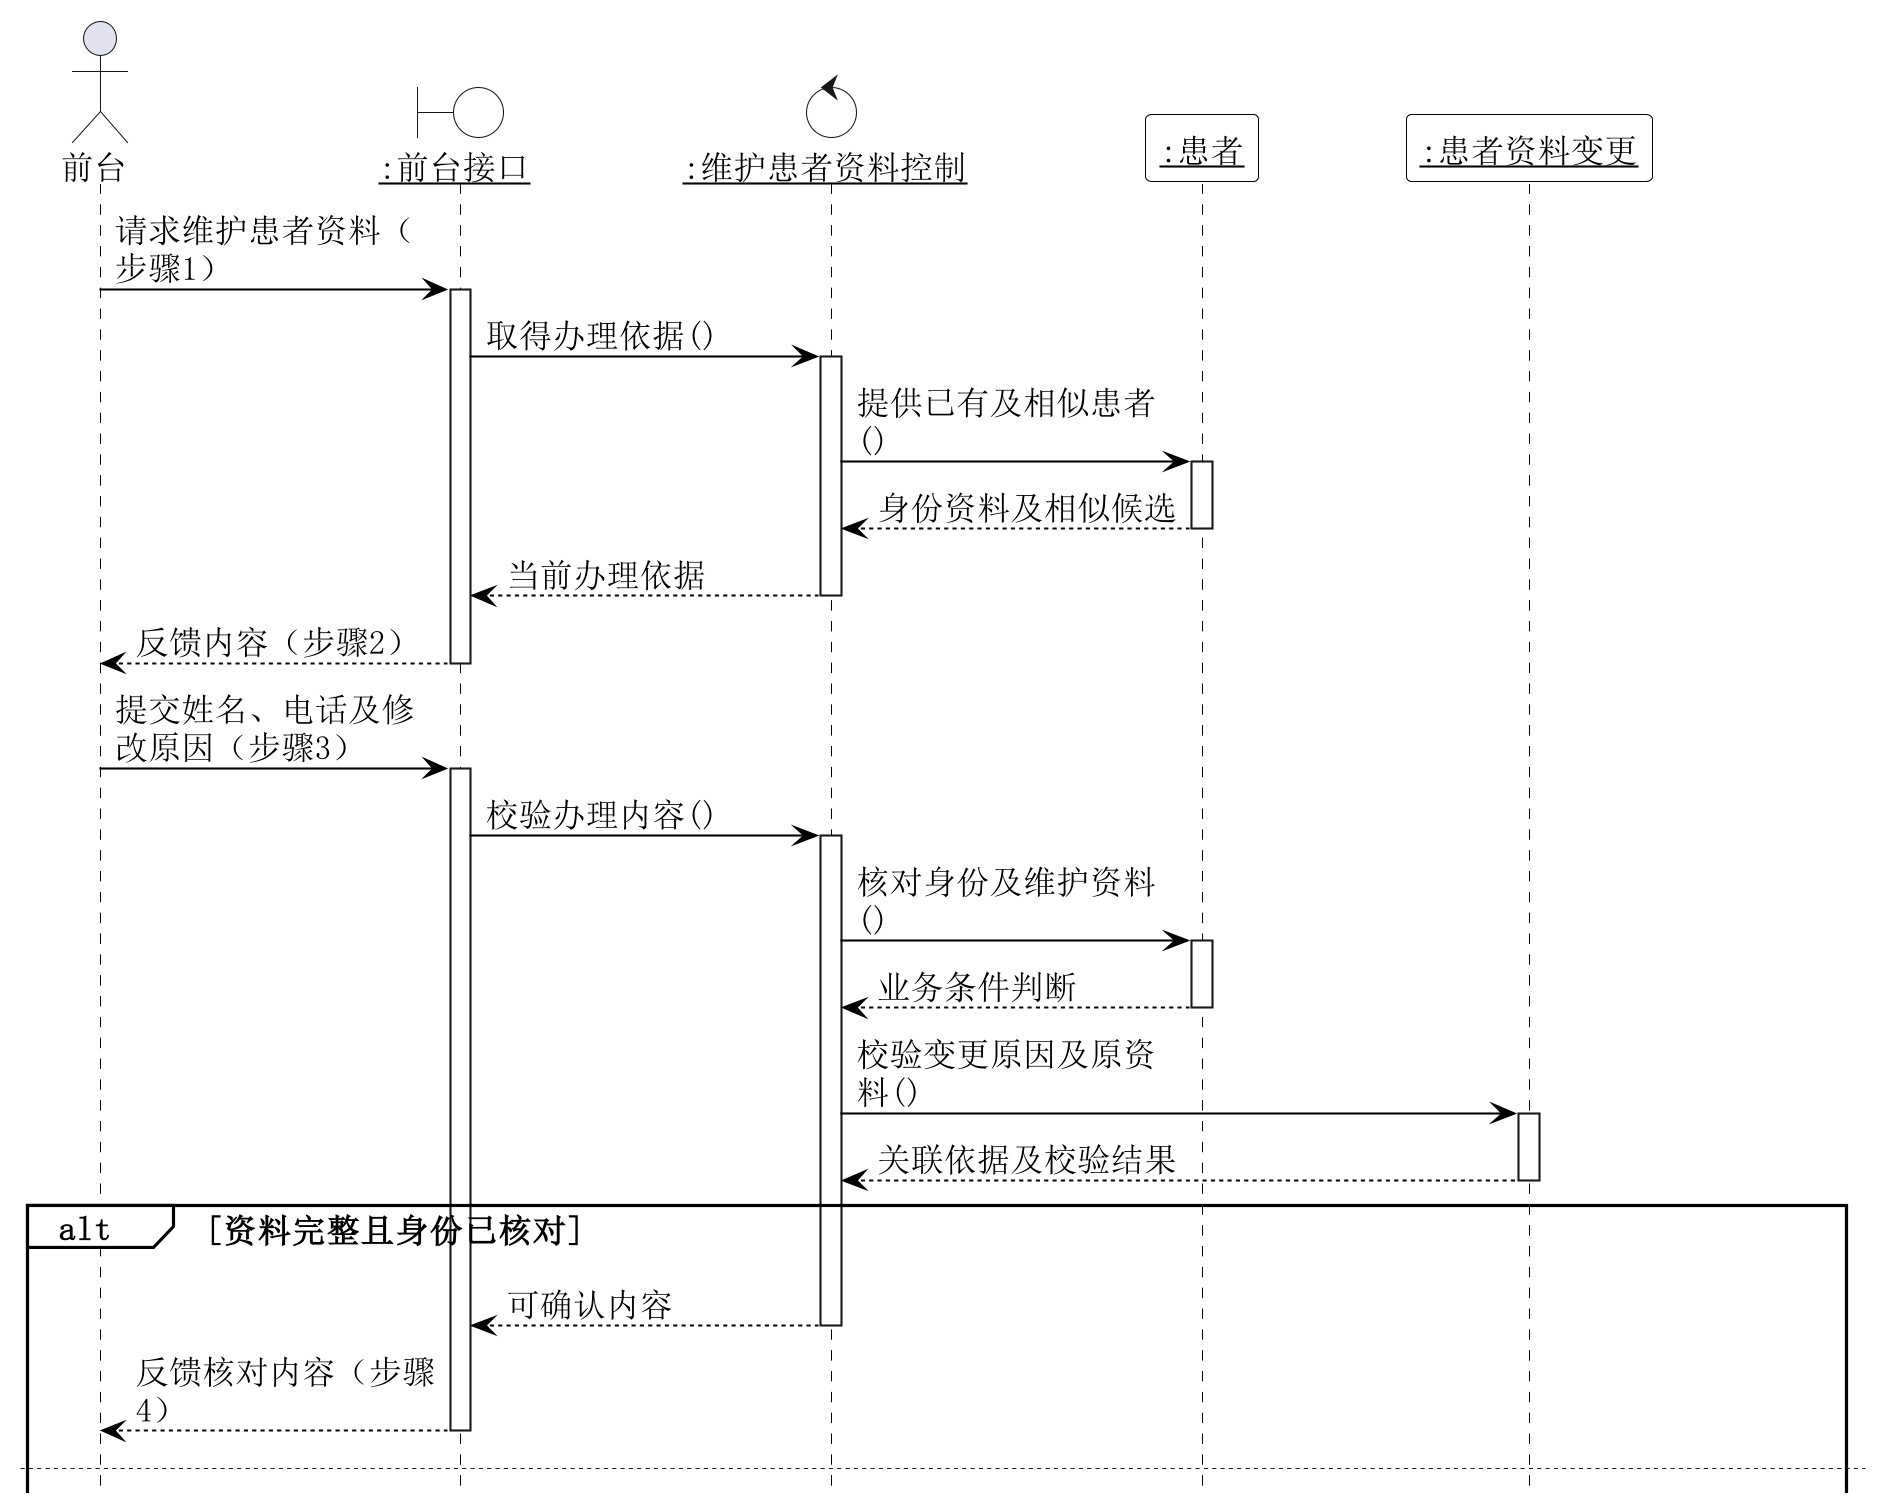
\includegraphics[width=\textwidth,height=20cm,keepaspectratio]{diagrams/13-08-analysis-sequence.png}
\caption{UC-08 维护患者资料分析序列图}
\label{fig:seq-08}
\end{figure}
\clearpage
\noindent\textbf{UC-08 分析序列图（续）}
\begin{figure}[!htbp]
\centering
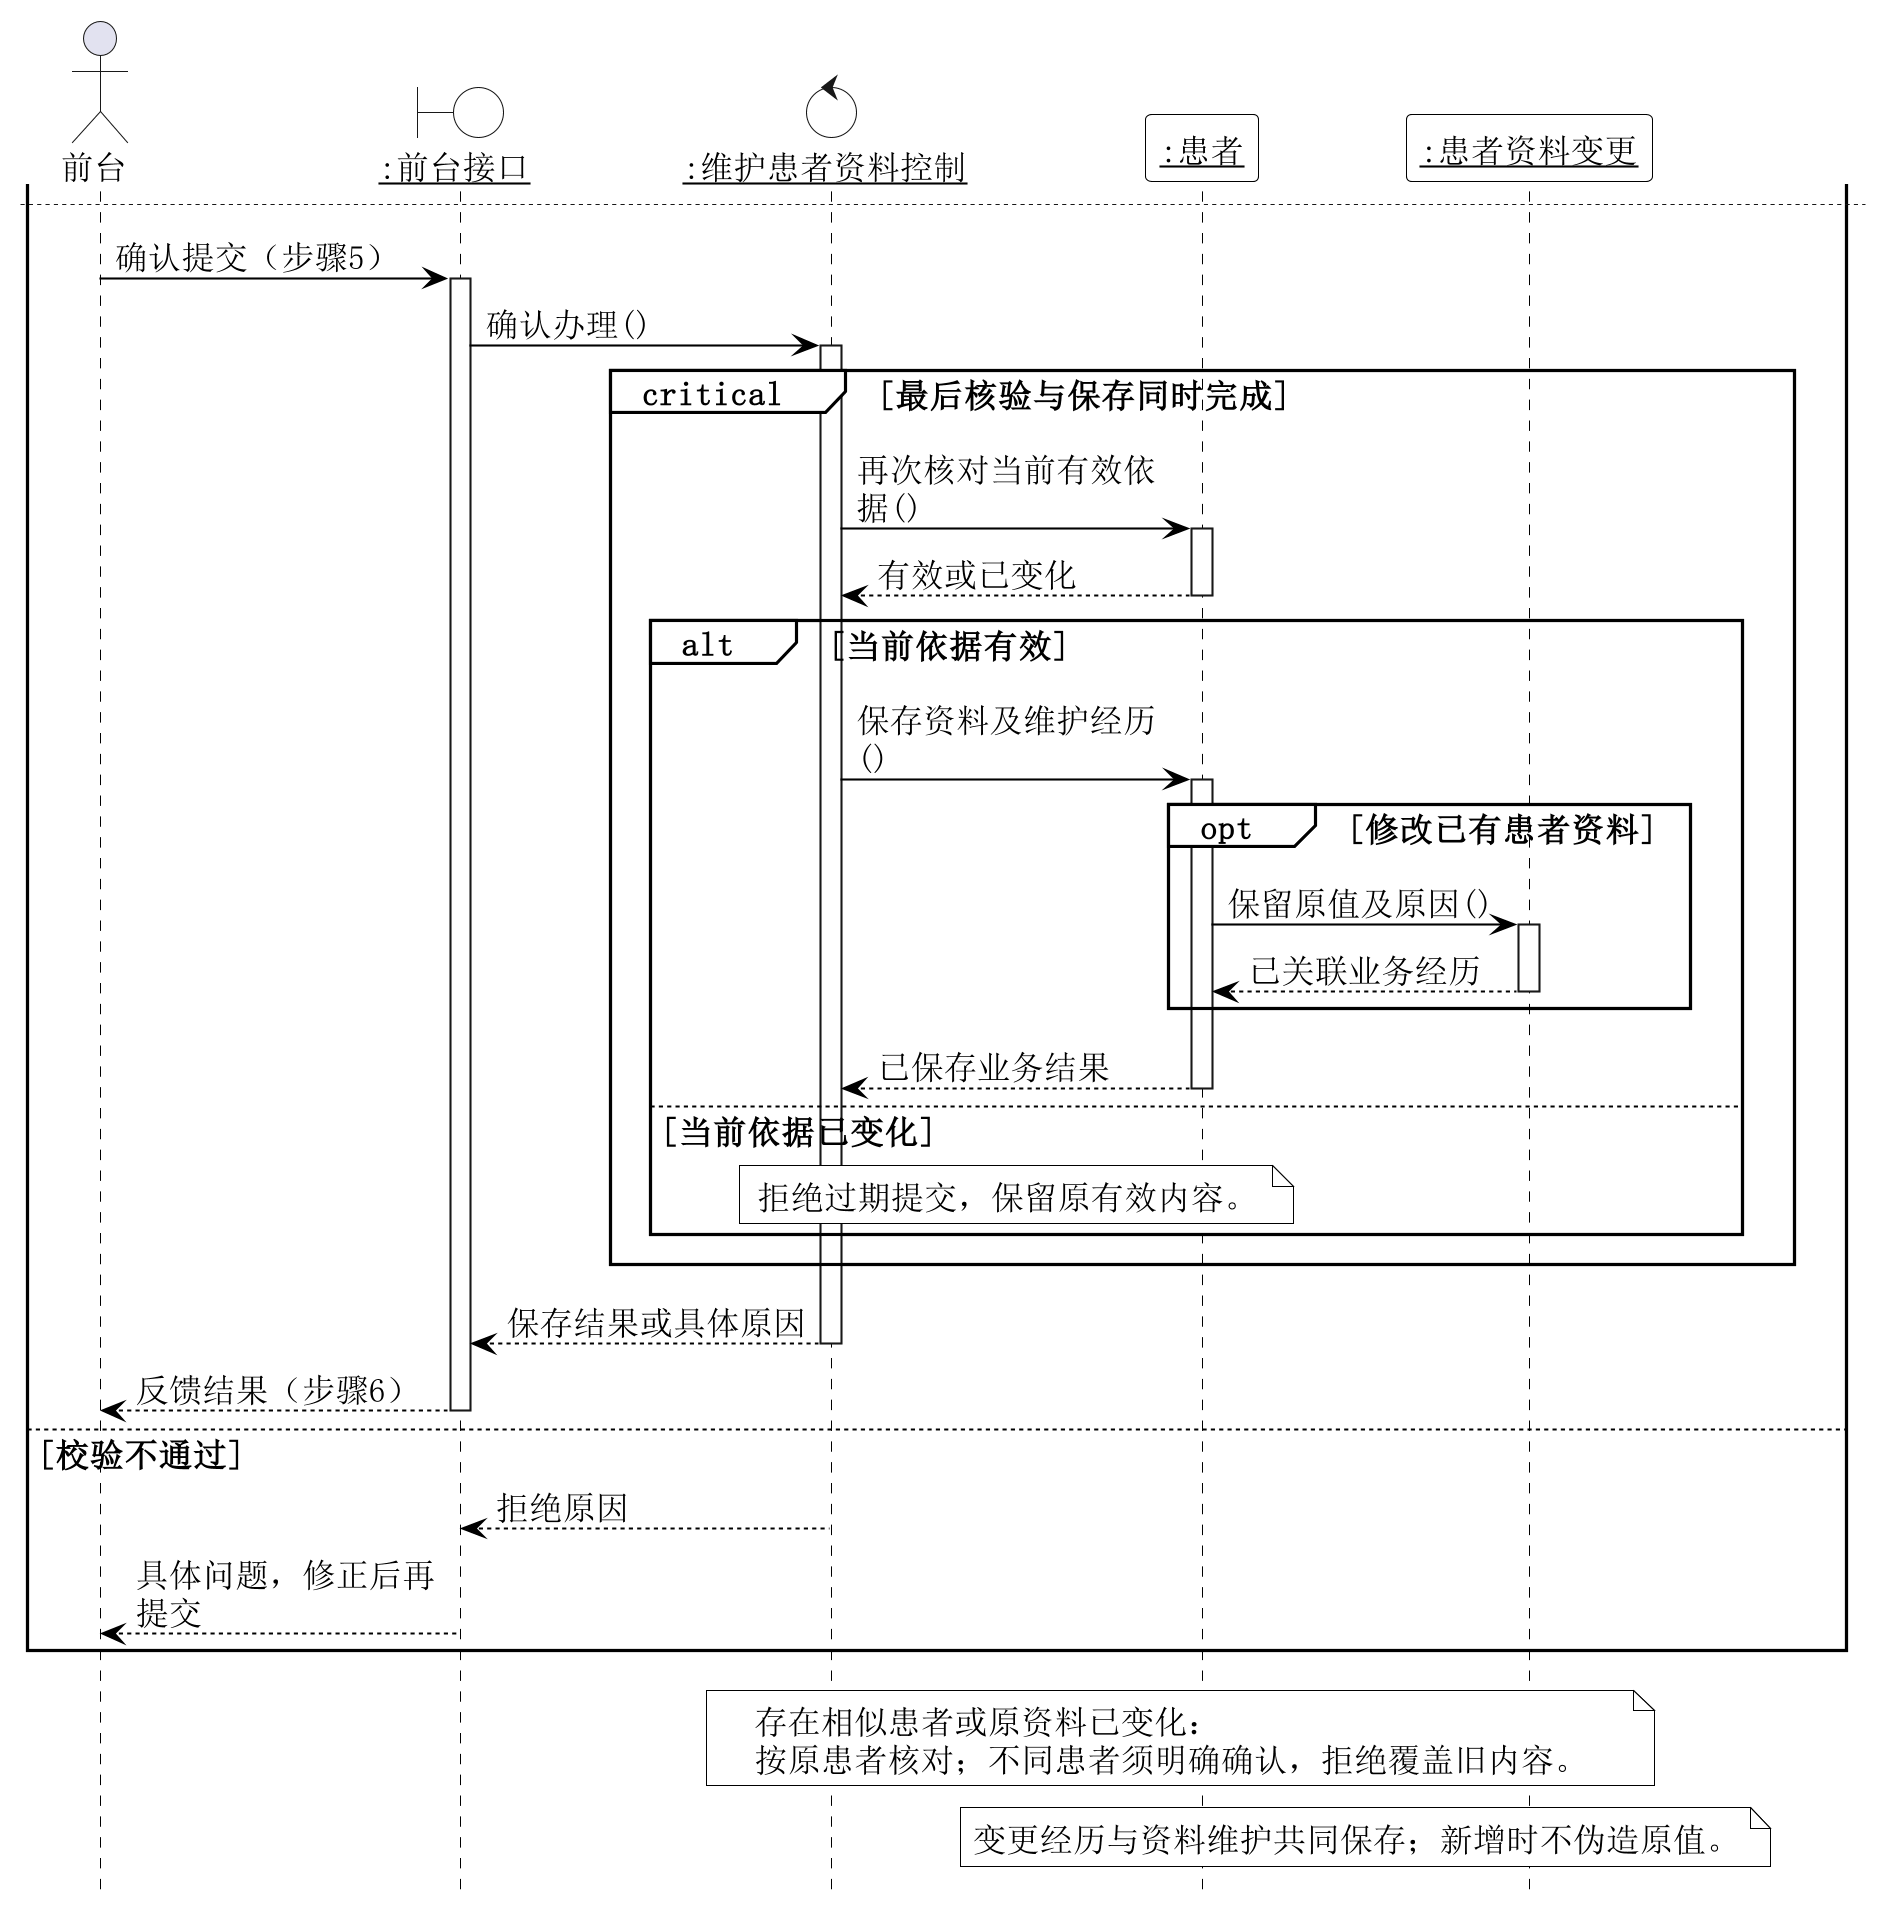
\includegraphics[width=\textwidth,height=20.4cm,keepaspectratio]{diagrams/13-08-analysis-sequence_001.png}
{\normalsize 图\ref{fig:seq-08}（续）：确认与保存}
\end{figure}
\clearpage
\subsubsection{UC-09：查询患者诊疗资料}

本图按规约分配就诊、患者、病历、病历补充的业务责任。
\begin{figure}[!htbp]
\centering
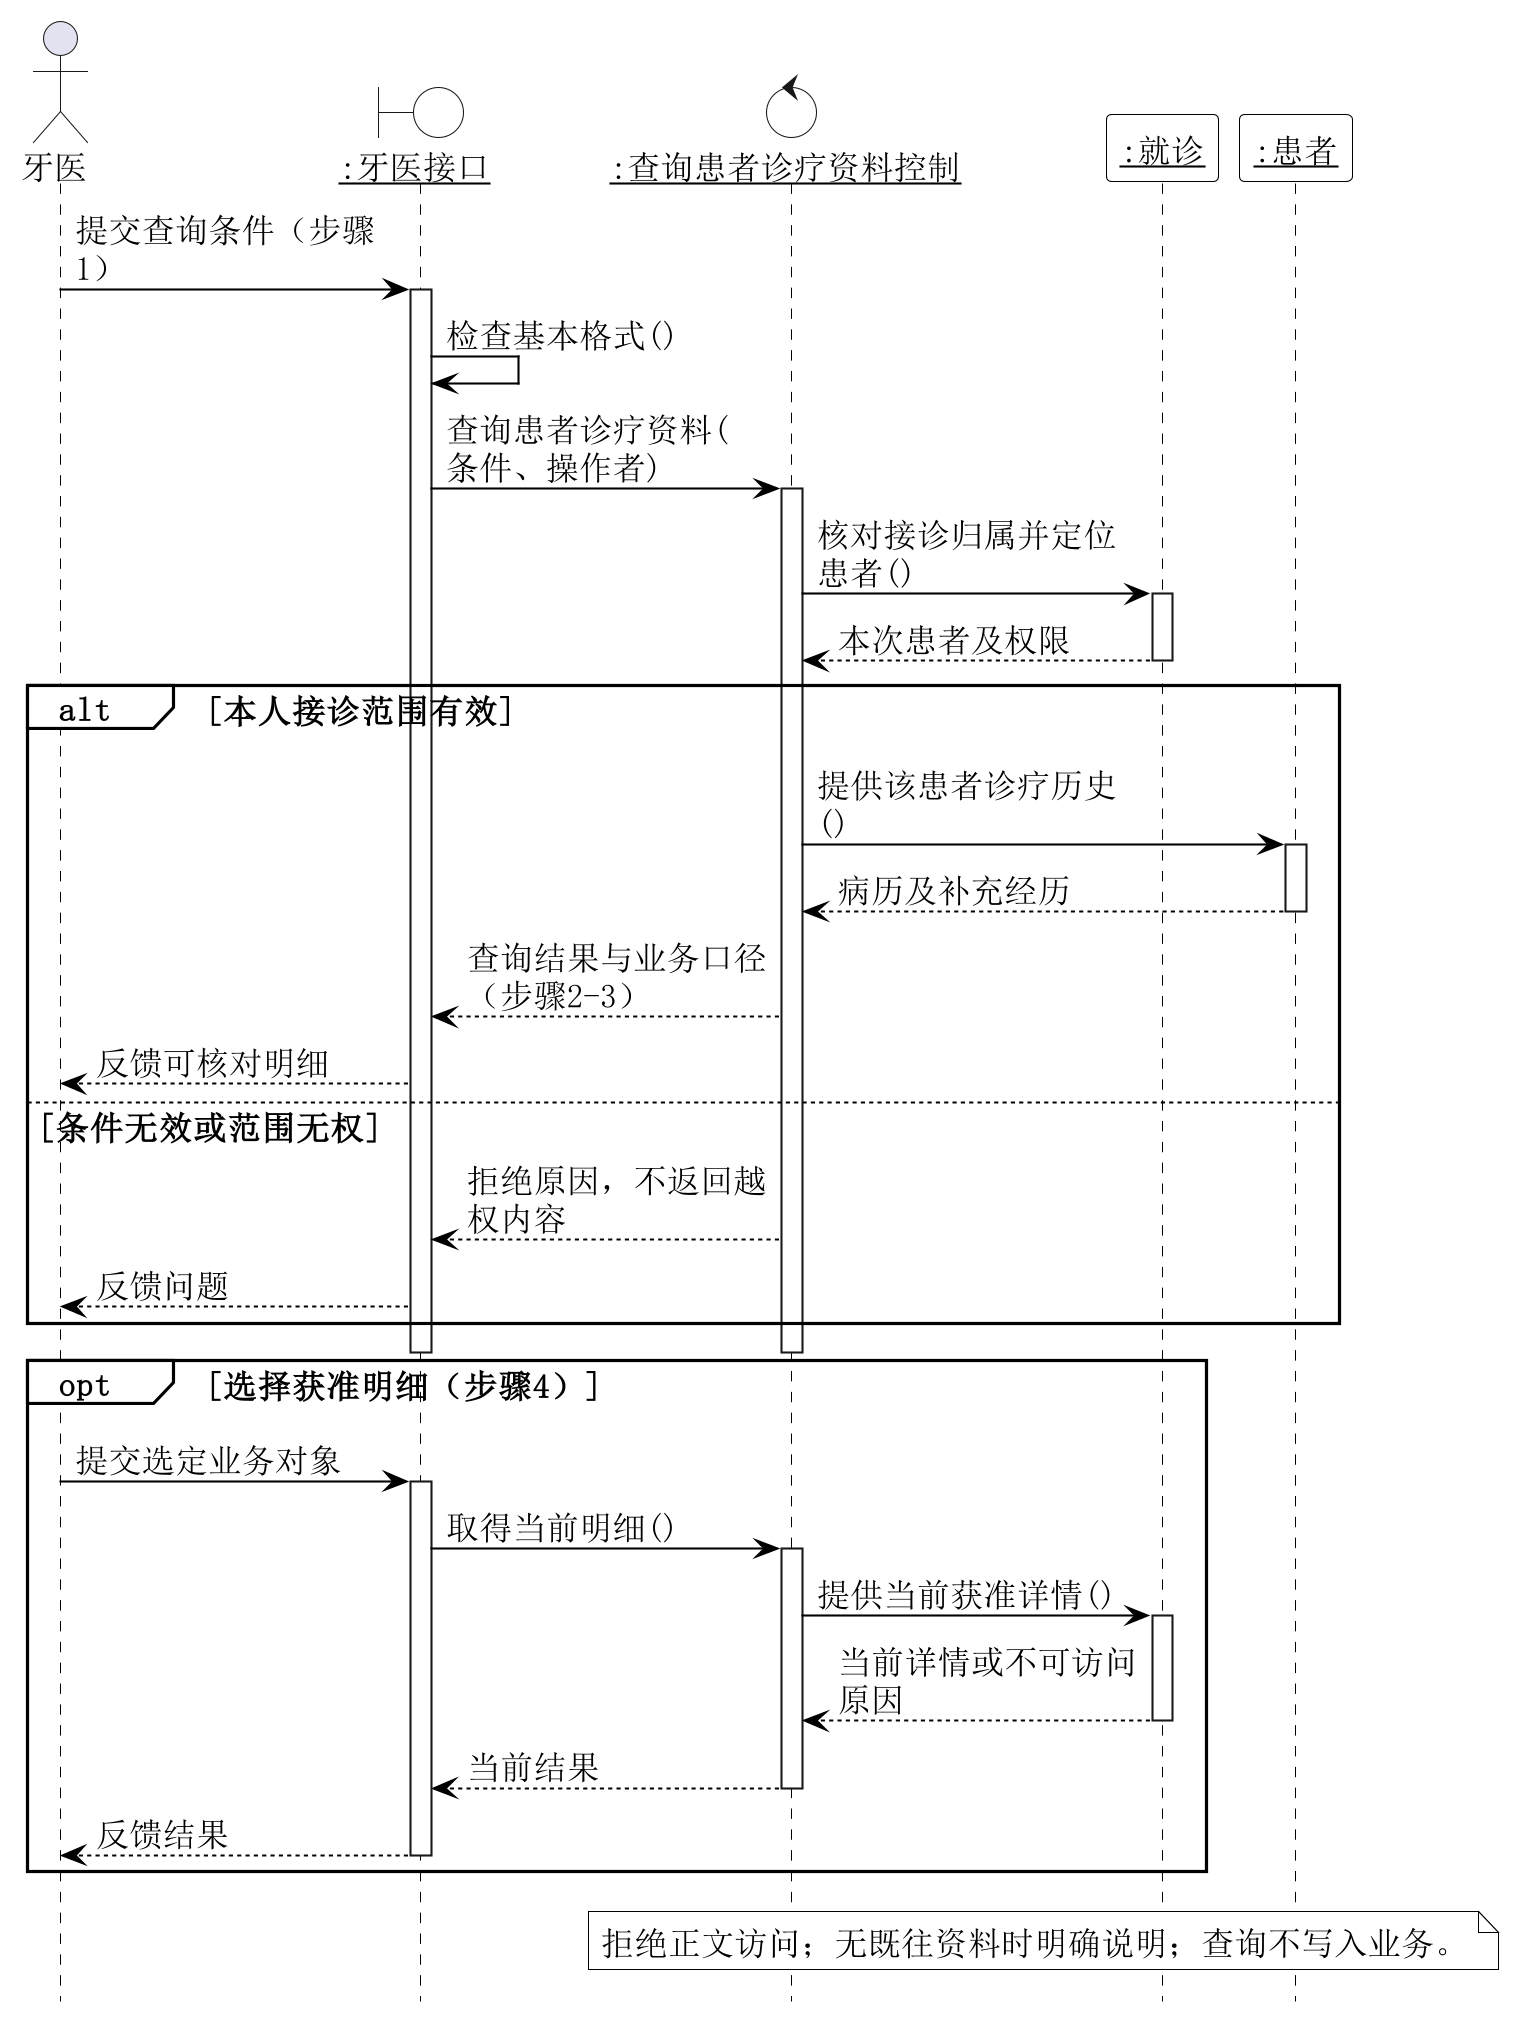
\includegraphics[width=\textwidth,height=20cm,keepaspectratio]{diagrams/13-09-analysis-sequence.png}
\caption{UC-09 查询患者诊疗资料分析序列图}
\label{fig:seq-09}
\end{figure}
\clearpage
\subsubsection{UC-10：记录检查诊断及方案}

本图按规约分配就诊、病历、检查所见、诊疗方案、方案项目的业务责任。
\begin{figure}[!htbp]
\centering
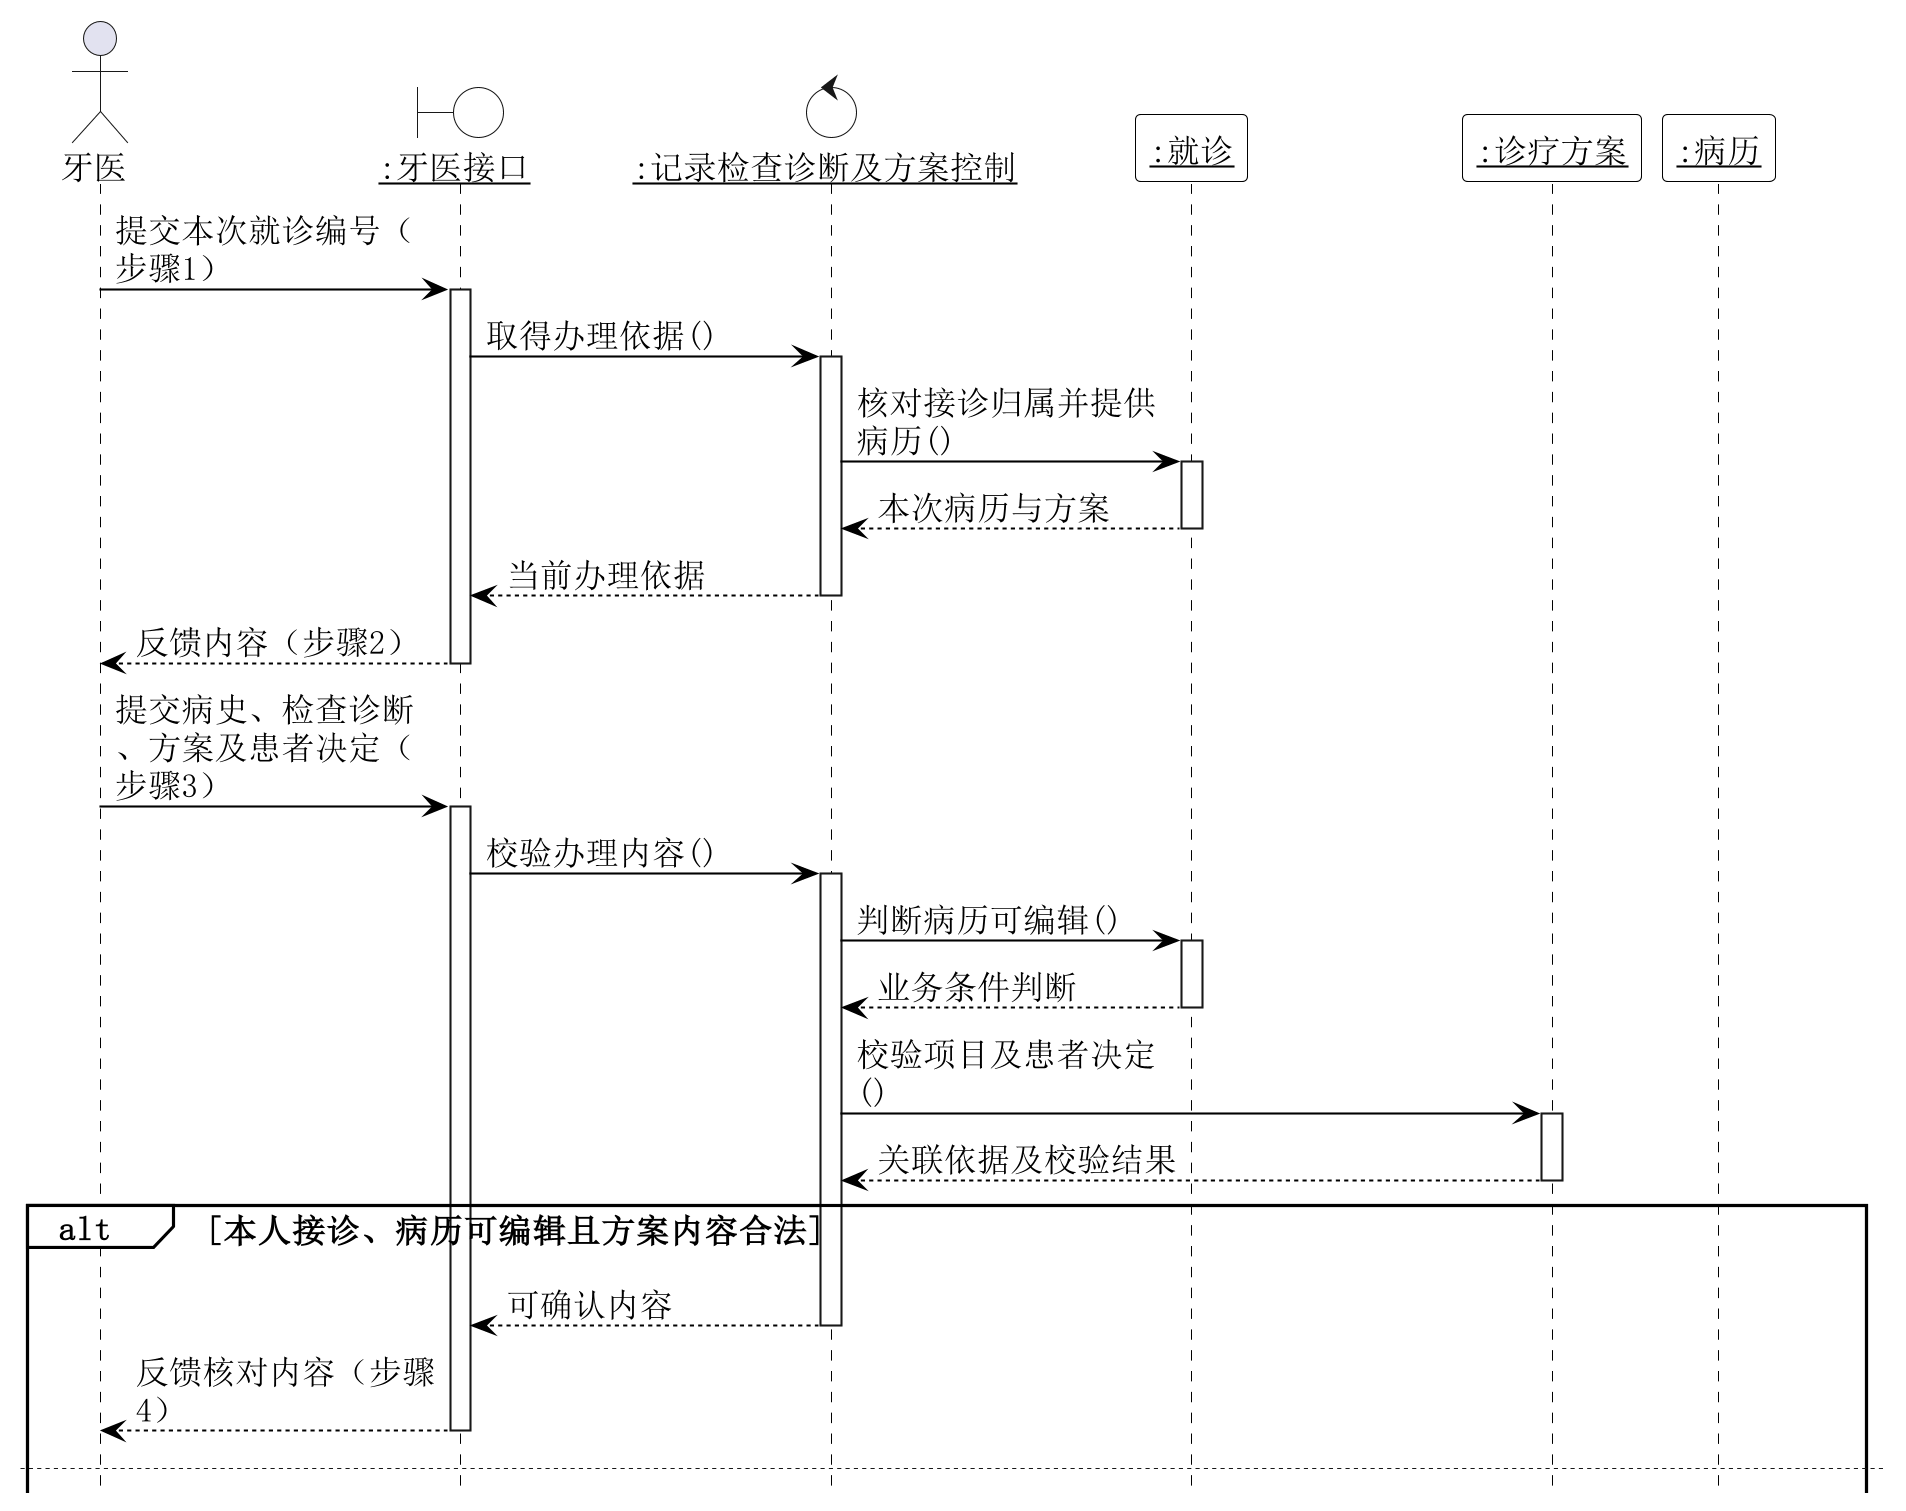
\includegraphics[width=\textwidth,height=20cm,keepaspectratio]{diagrams/13-10-analysis-sequence.png}
\caption{UC-10 记录检查诊断及方案分析序列图}
\label{fig:seq-10}
\end{figure}
\clearpage
\noindent\textbf{UC-10 分析序列图（续）}
\begin{figure}[!htbp]
\centering
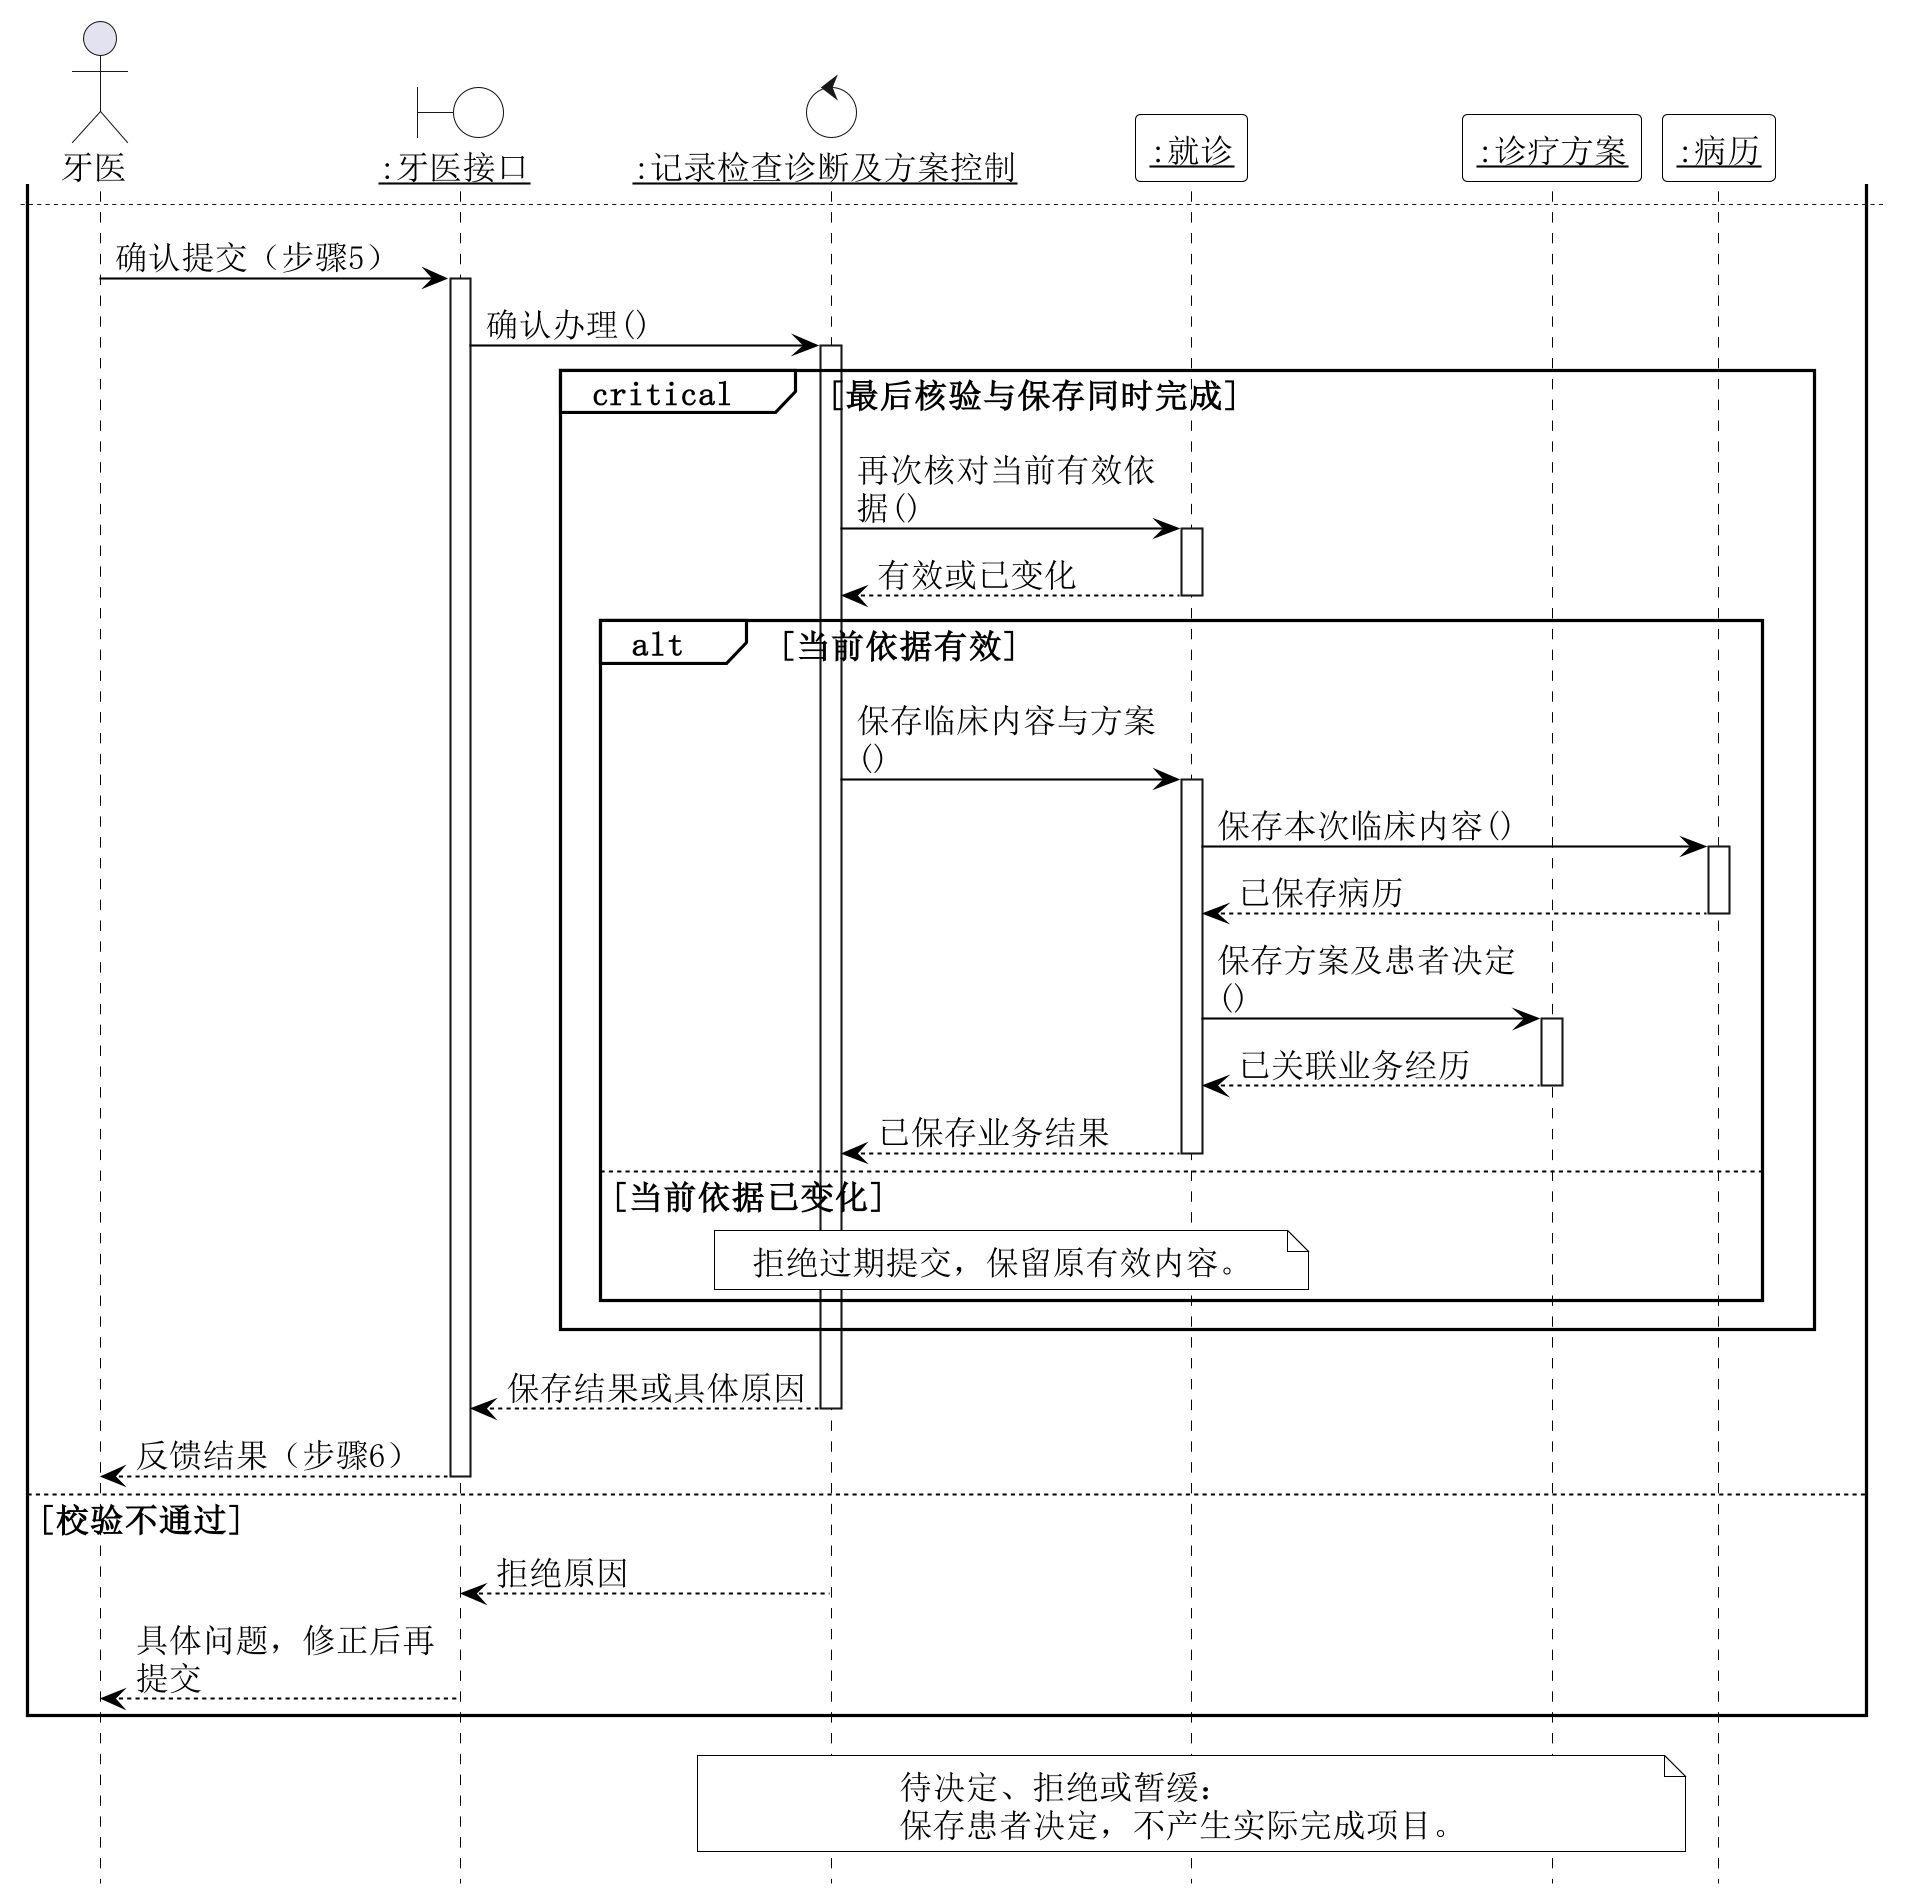
\includegraphics[width=\textwidth,height=20.4cm,keepaspectratio]{diagrams/13-10-analysis-sequence_001.png}
{\normalsize 图\ref{fig:seq-10}（续）：确认与保存}
\end{figure}
\clearpage
\subsubsection{UC-11：签署及补充病历}

本图按规约分配就诊、病历、病历补充、诊疗确认的业务责任。
\begin{figure}[!htbp]
\centering
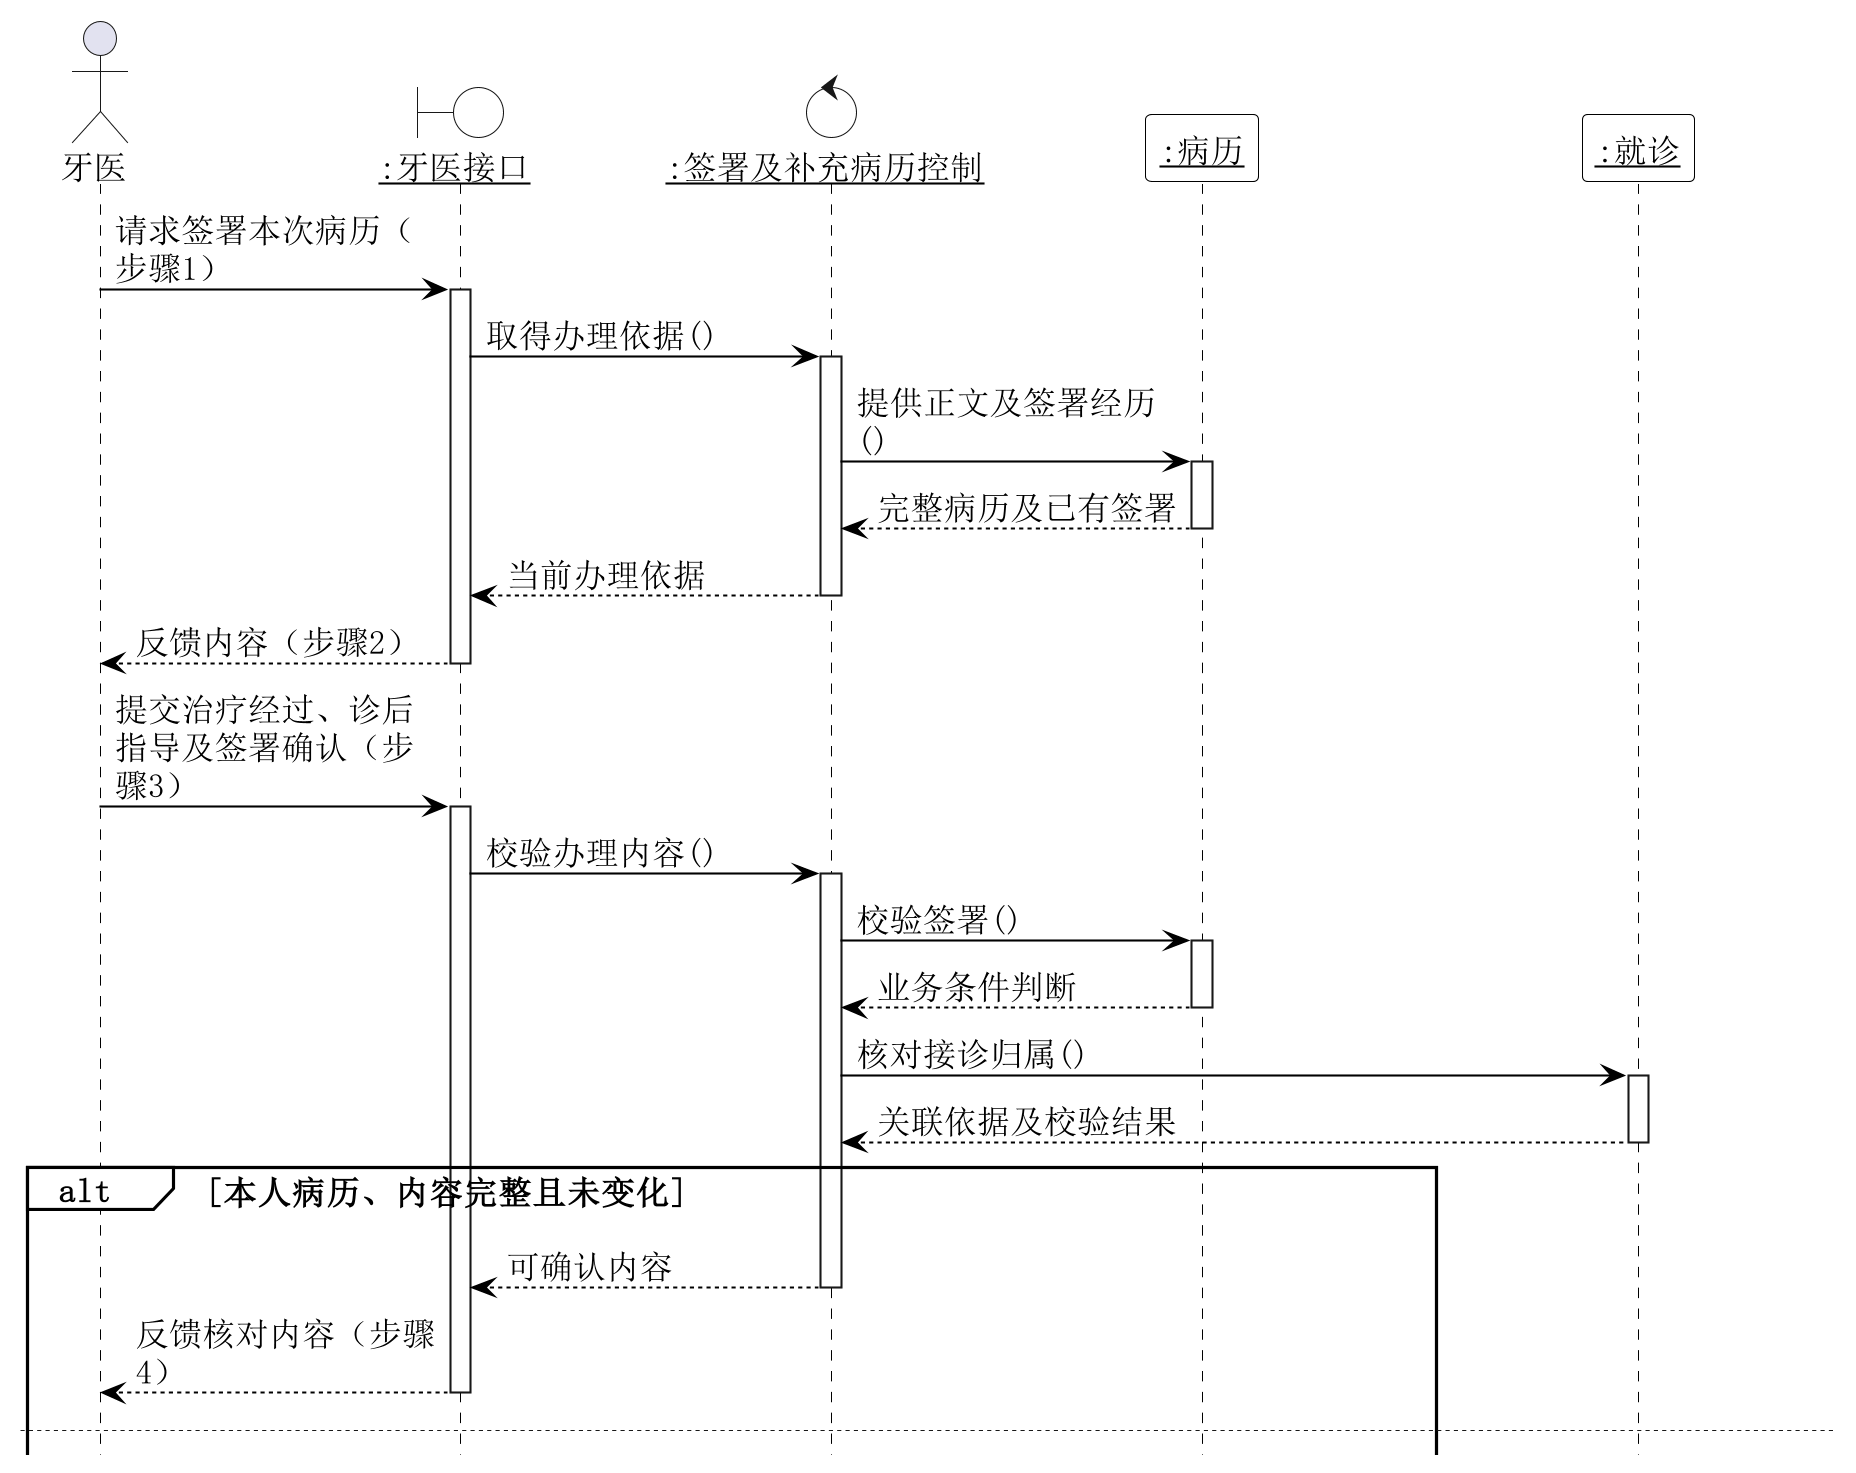
\includegraphics[width=\textwidth,height=20cm,keepaspectratio]{diagrams/13-11-analysis-sequence.png}
\caption{UC-11 签署及补充病历分析序列图}
\label{fig:seq-11}
\end{figure}
\clearpage
\noindent\textbf{UC-11 分析序列图（续）}
\begin{figure}[!htbp]
\centering
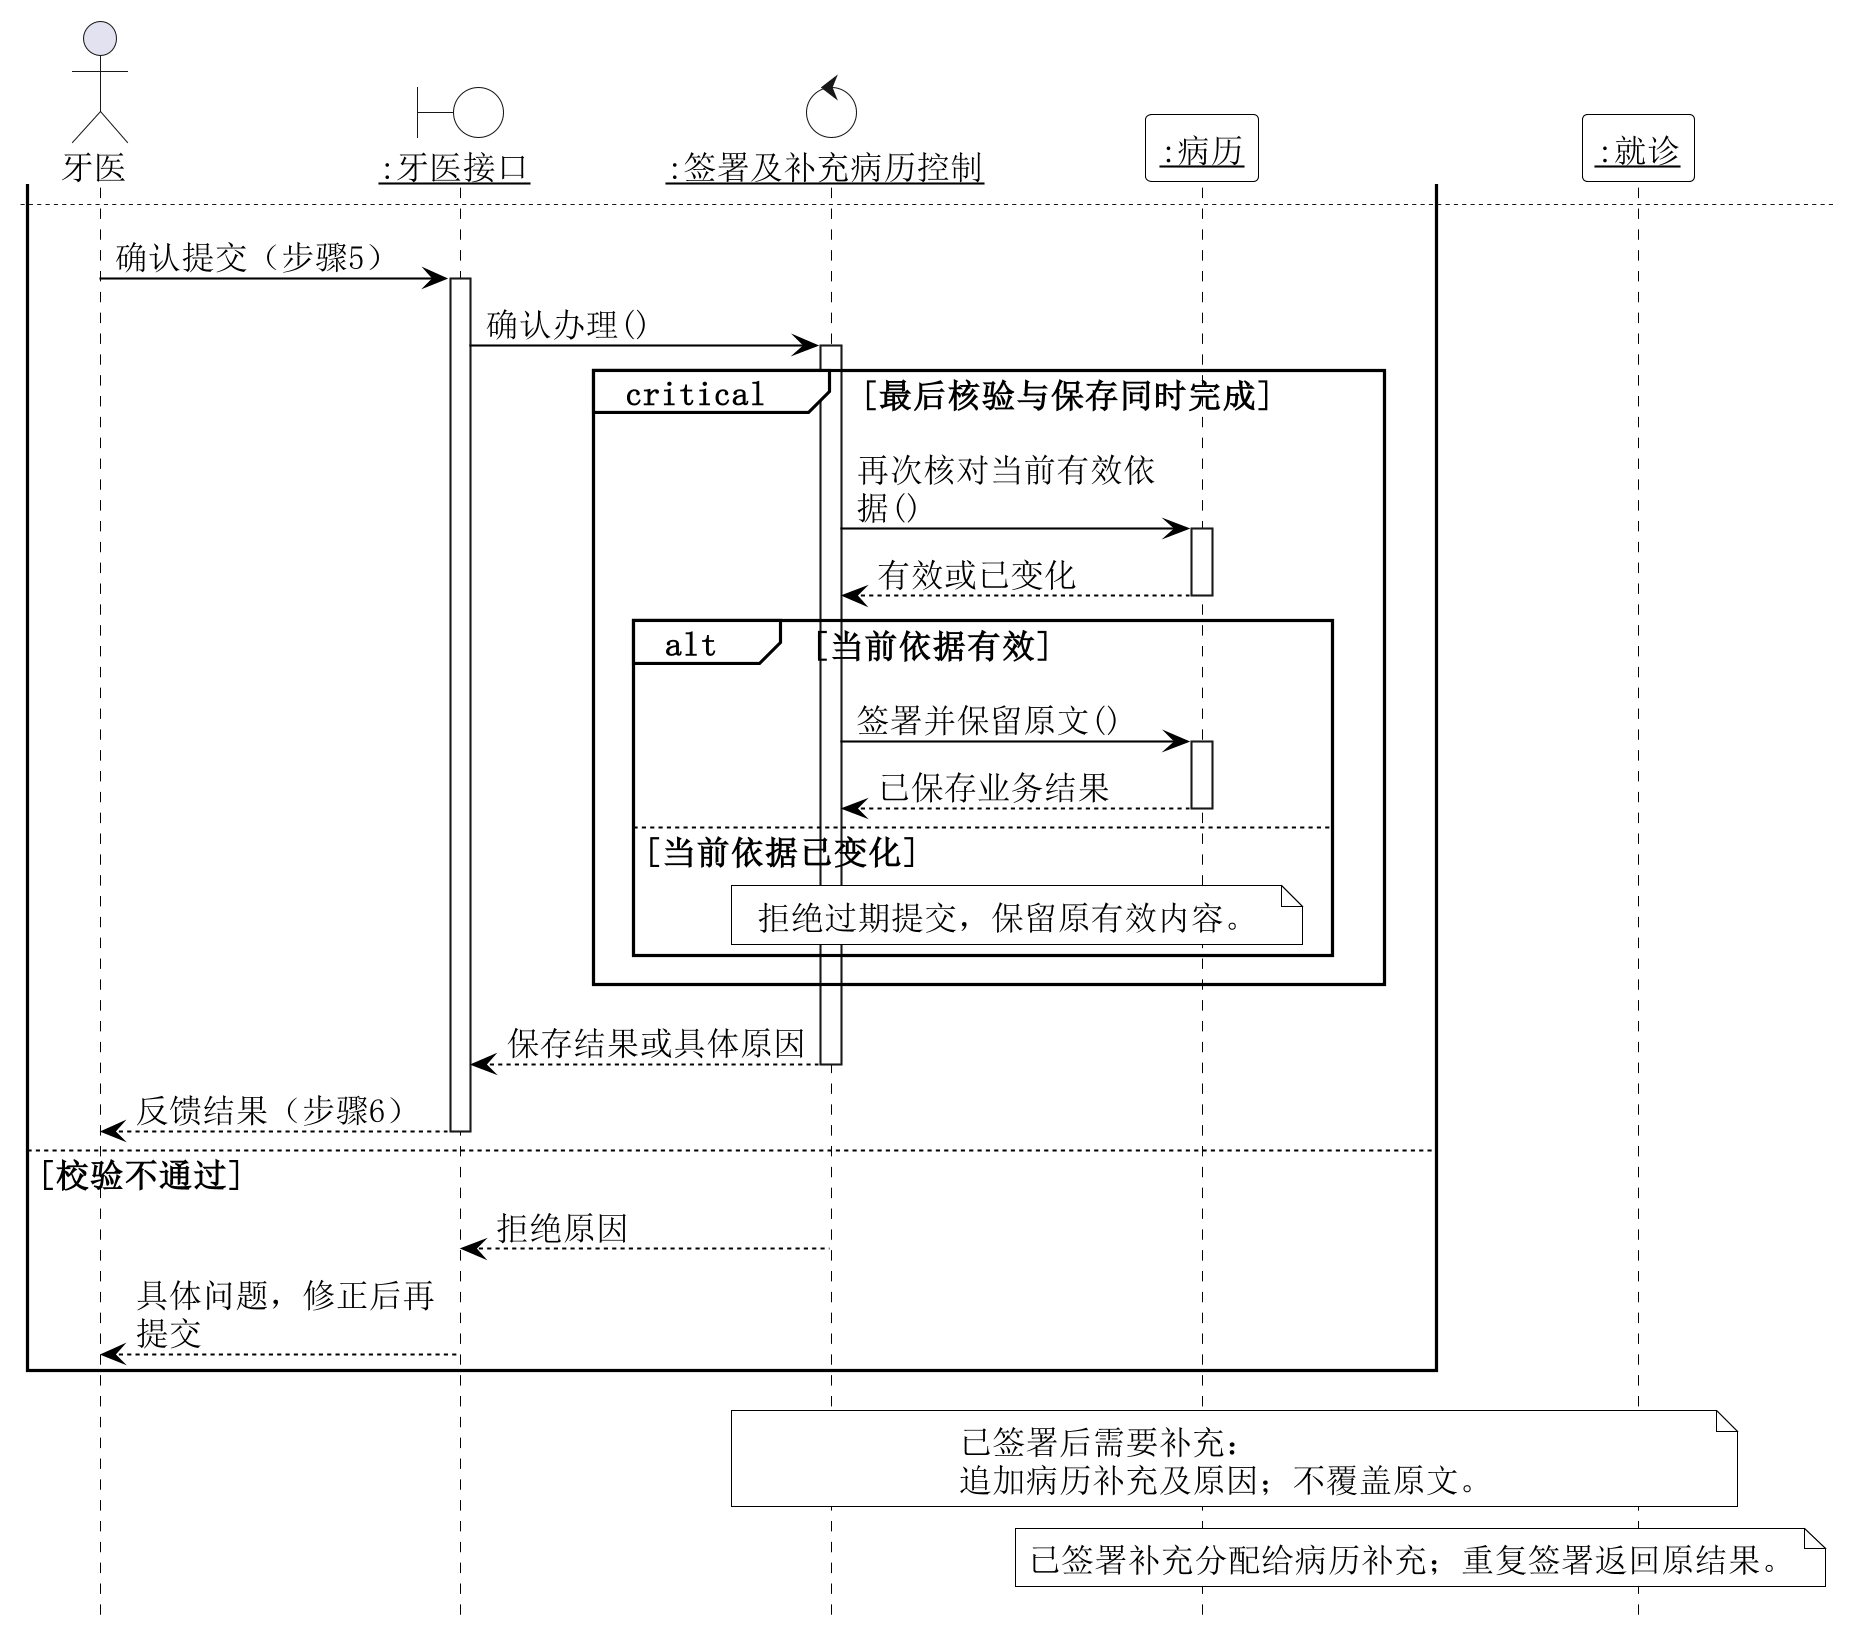
\includegraphics[width=\textwidth,height=20.4cm,keepaspectratio]{diagrams/13-11-analysis-sequence_001.png}
{\normalsize 图\ref{fig:seq-11}（续）：确认与保存}
\end{figure}
\clearpage
\noindent\textbf{UC-11：补充已签署病历}
\begin{figure}[!htbp]
\centering
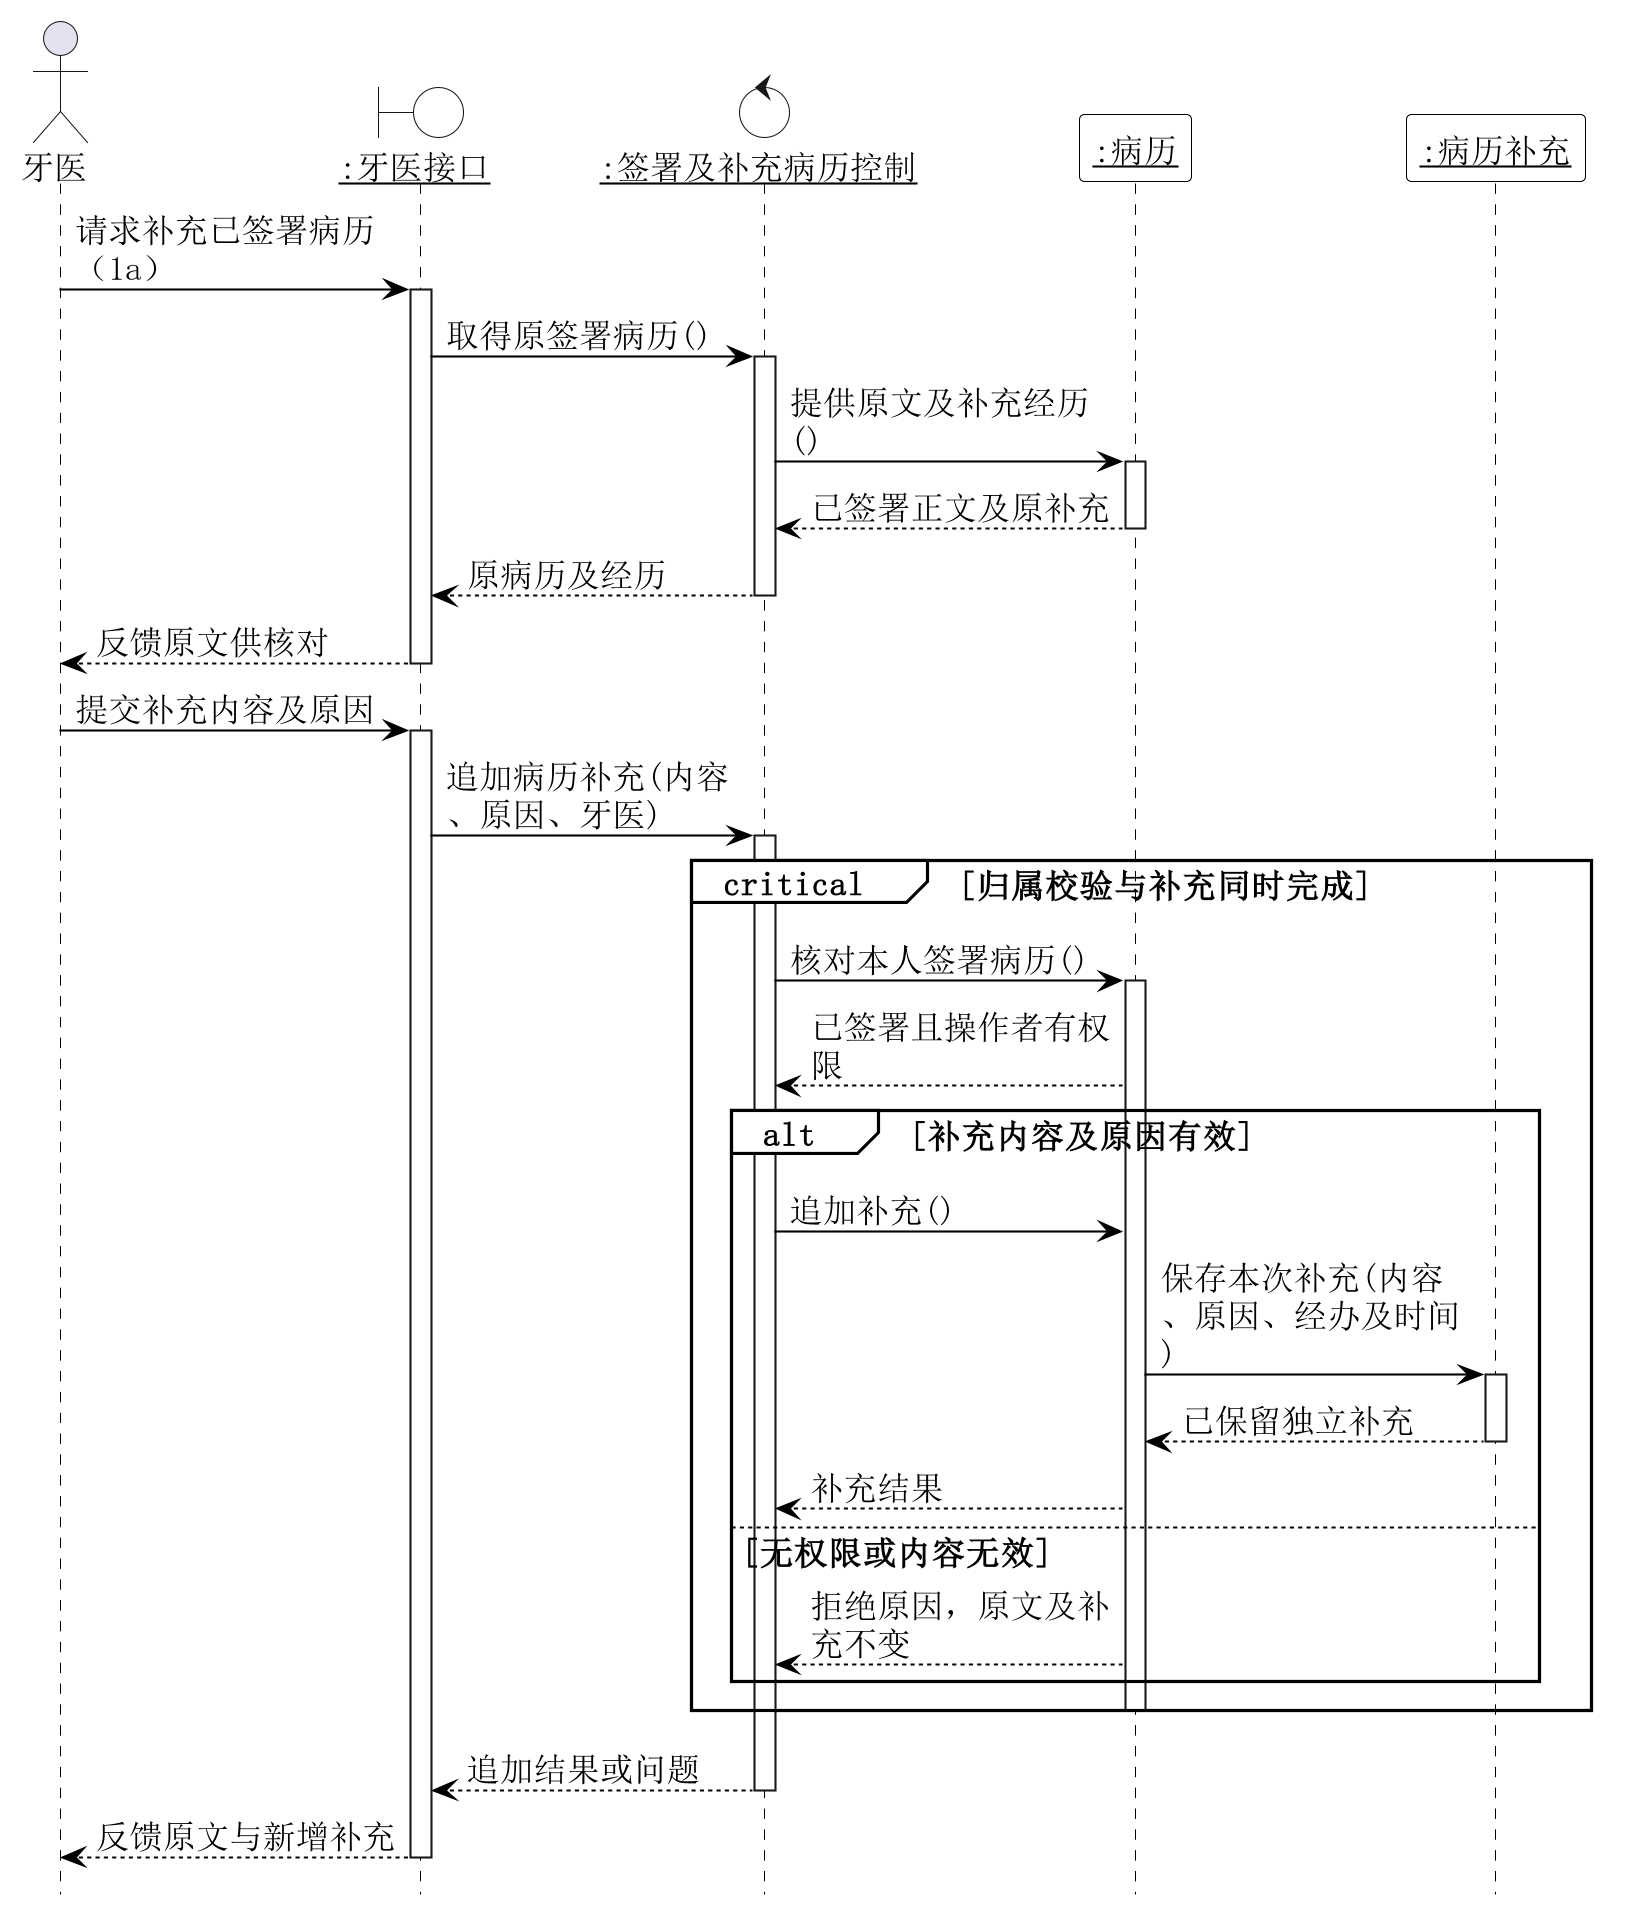
\includegraphics[width=\textwidth,height=20cm,keepaspectratio]{diagrams/13-11a-analysis-sequence.png}
\caption{UC-11 补充已签署病历分析序列图}
\label{fig:seq-11-ext}
\end{figure}
\clearpage
\subsubsection{UC-12：提出复诊随访要求}

本图按规约分配就诊、病历、诊后要求、职员的业务责任。
\begin{figure}[!htbp]
\centering
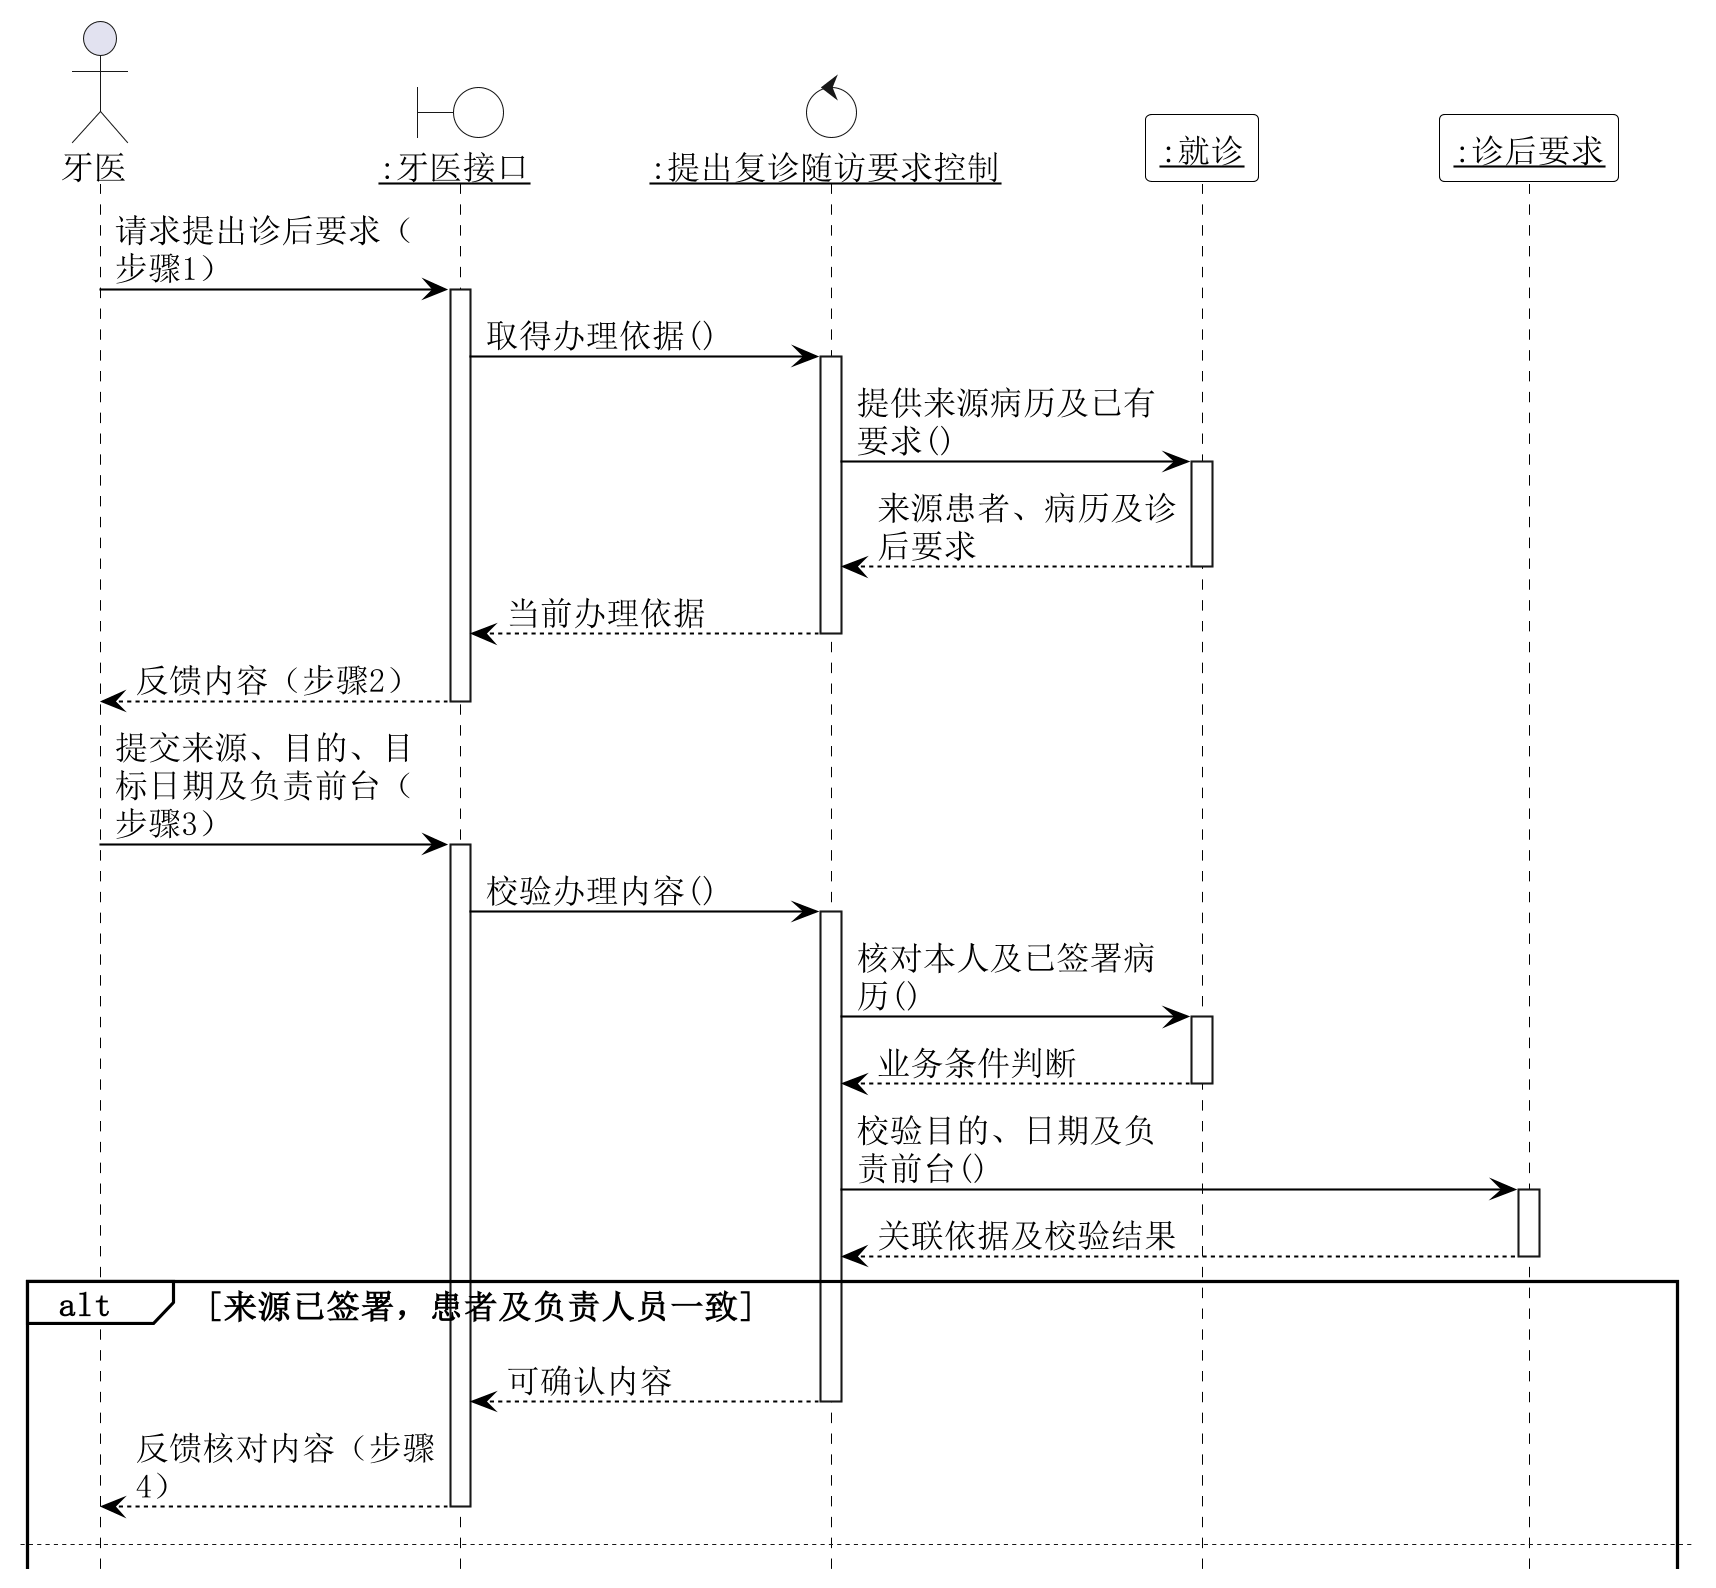
\includegraphics[width=\textwidth,height=20cm,keepaspectratio]{diagrams/13-12-analysis-sequence.png}
\caption{UC-12 提出复诊随访要求分析序列图}
\label{fig:seq-12}
\end{figure}
\clearpage
\noindent\textbf{UC-12 分析序列图（续）}
\begin{figure}[!htbp]
\centering
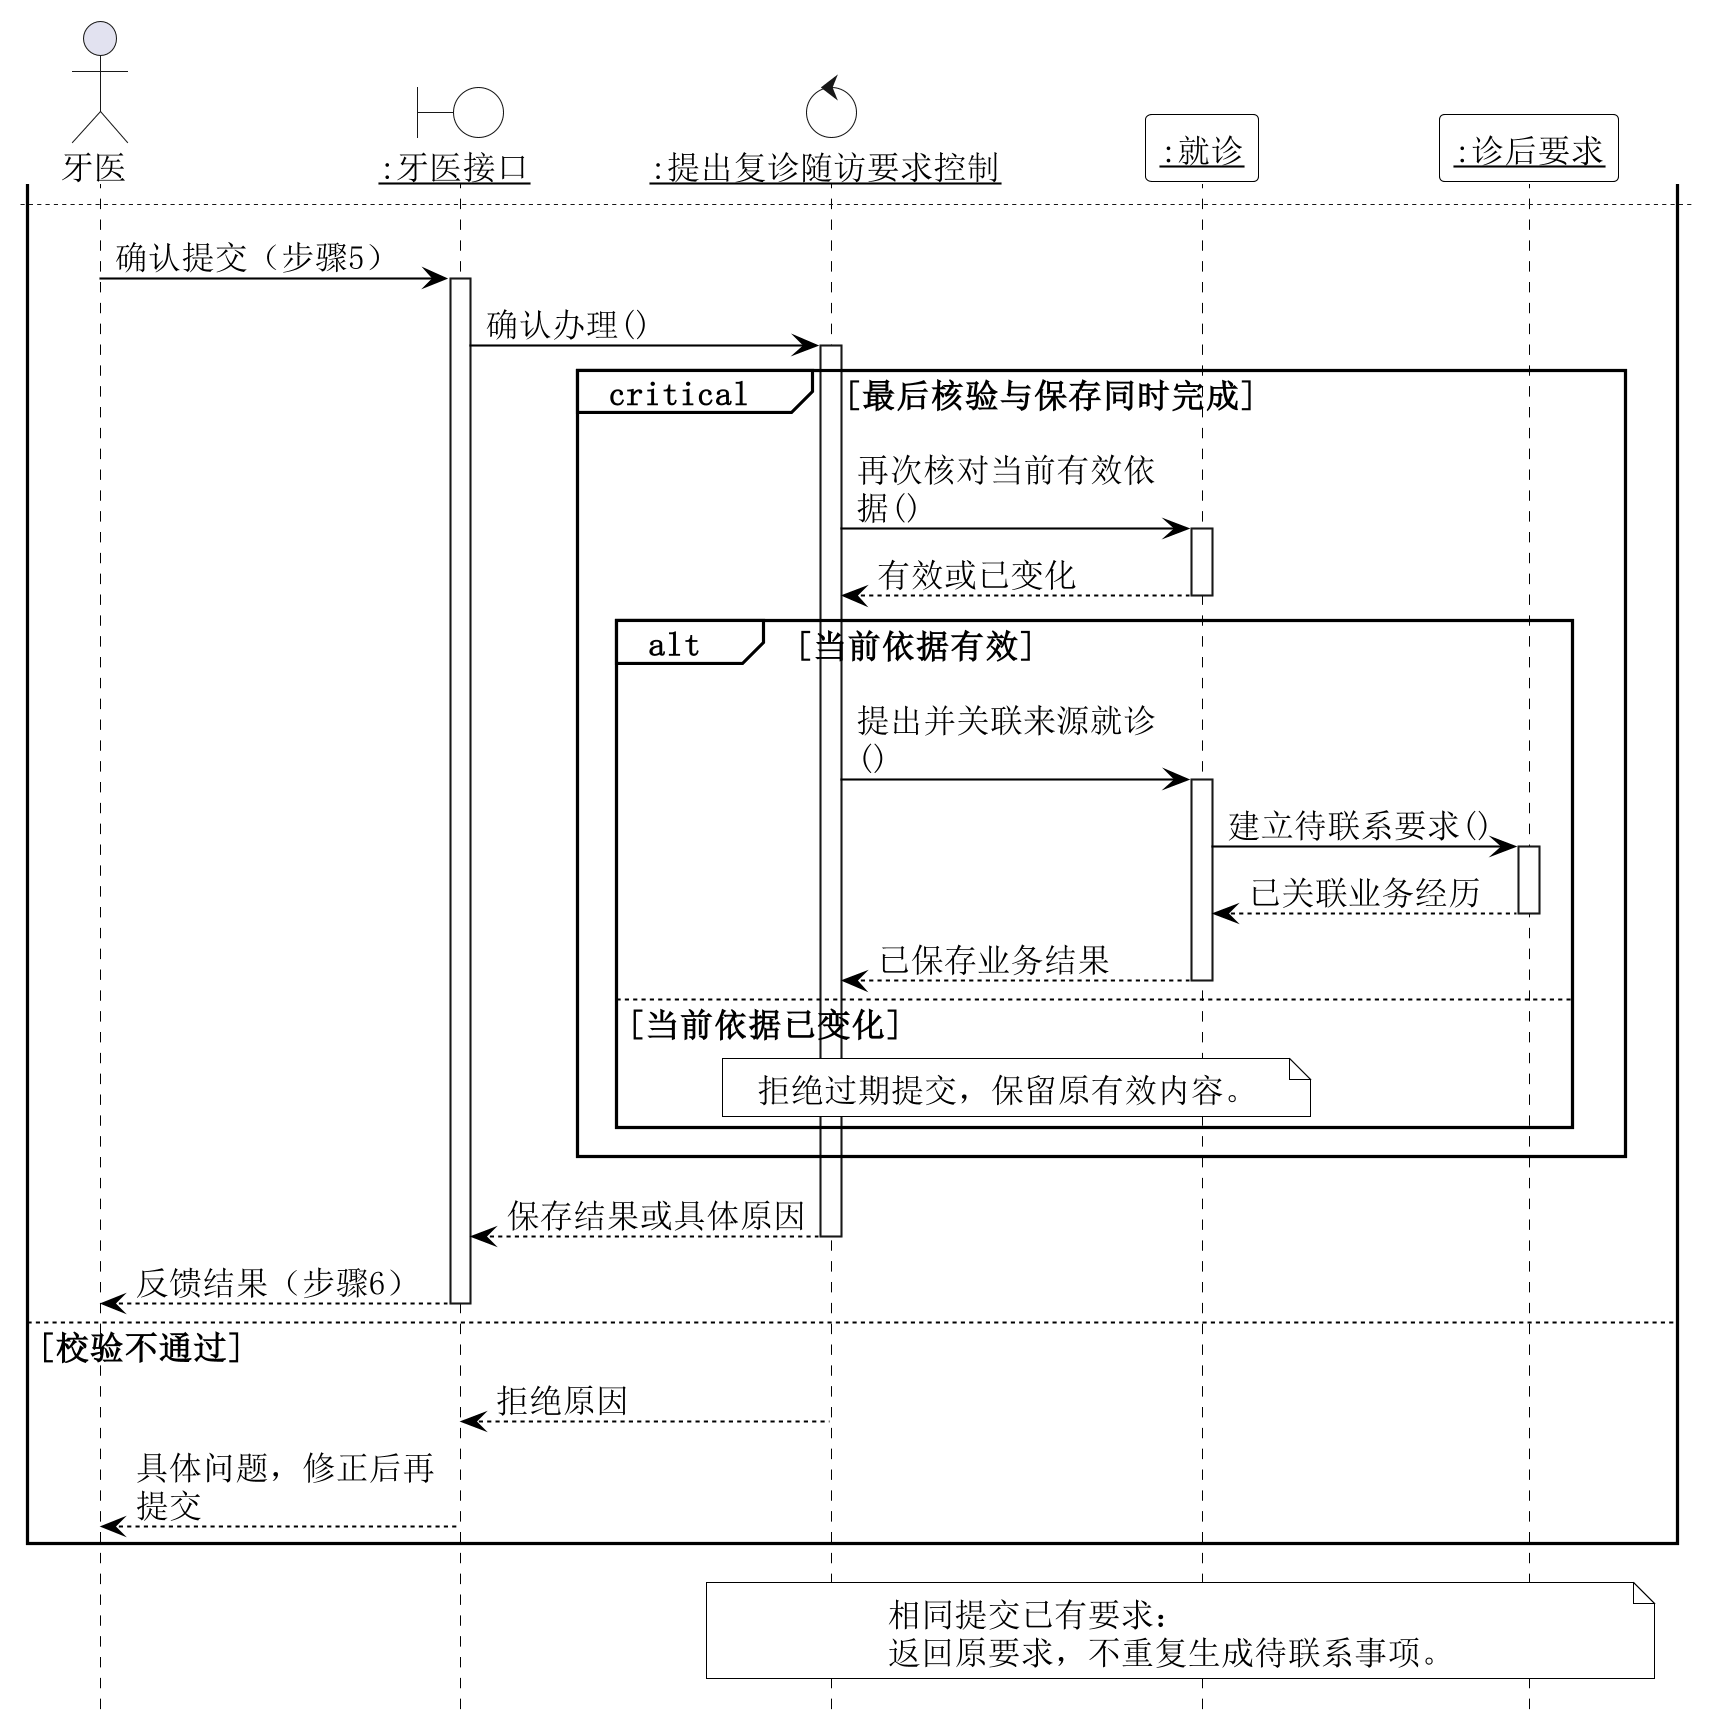
\includegraphics[width=\textwidth,height=20.4cm,keepaspectratio]{diagrams/13-12-analysis-sequence_001.png}
{\normalsize 图\ref{fig:seq-12}（续）：确认与保存}
\end{figure}
\clearpage
\subsubsection{UC-13：办理复诊随访联系}

本图按规约分配诊后要求、联系经历、预约、职员的业务责任。
\begin{figure}[!htbp]
\centering
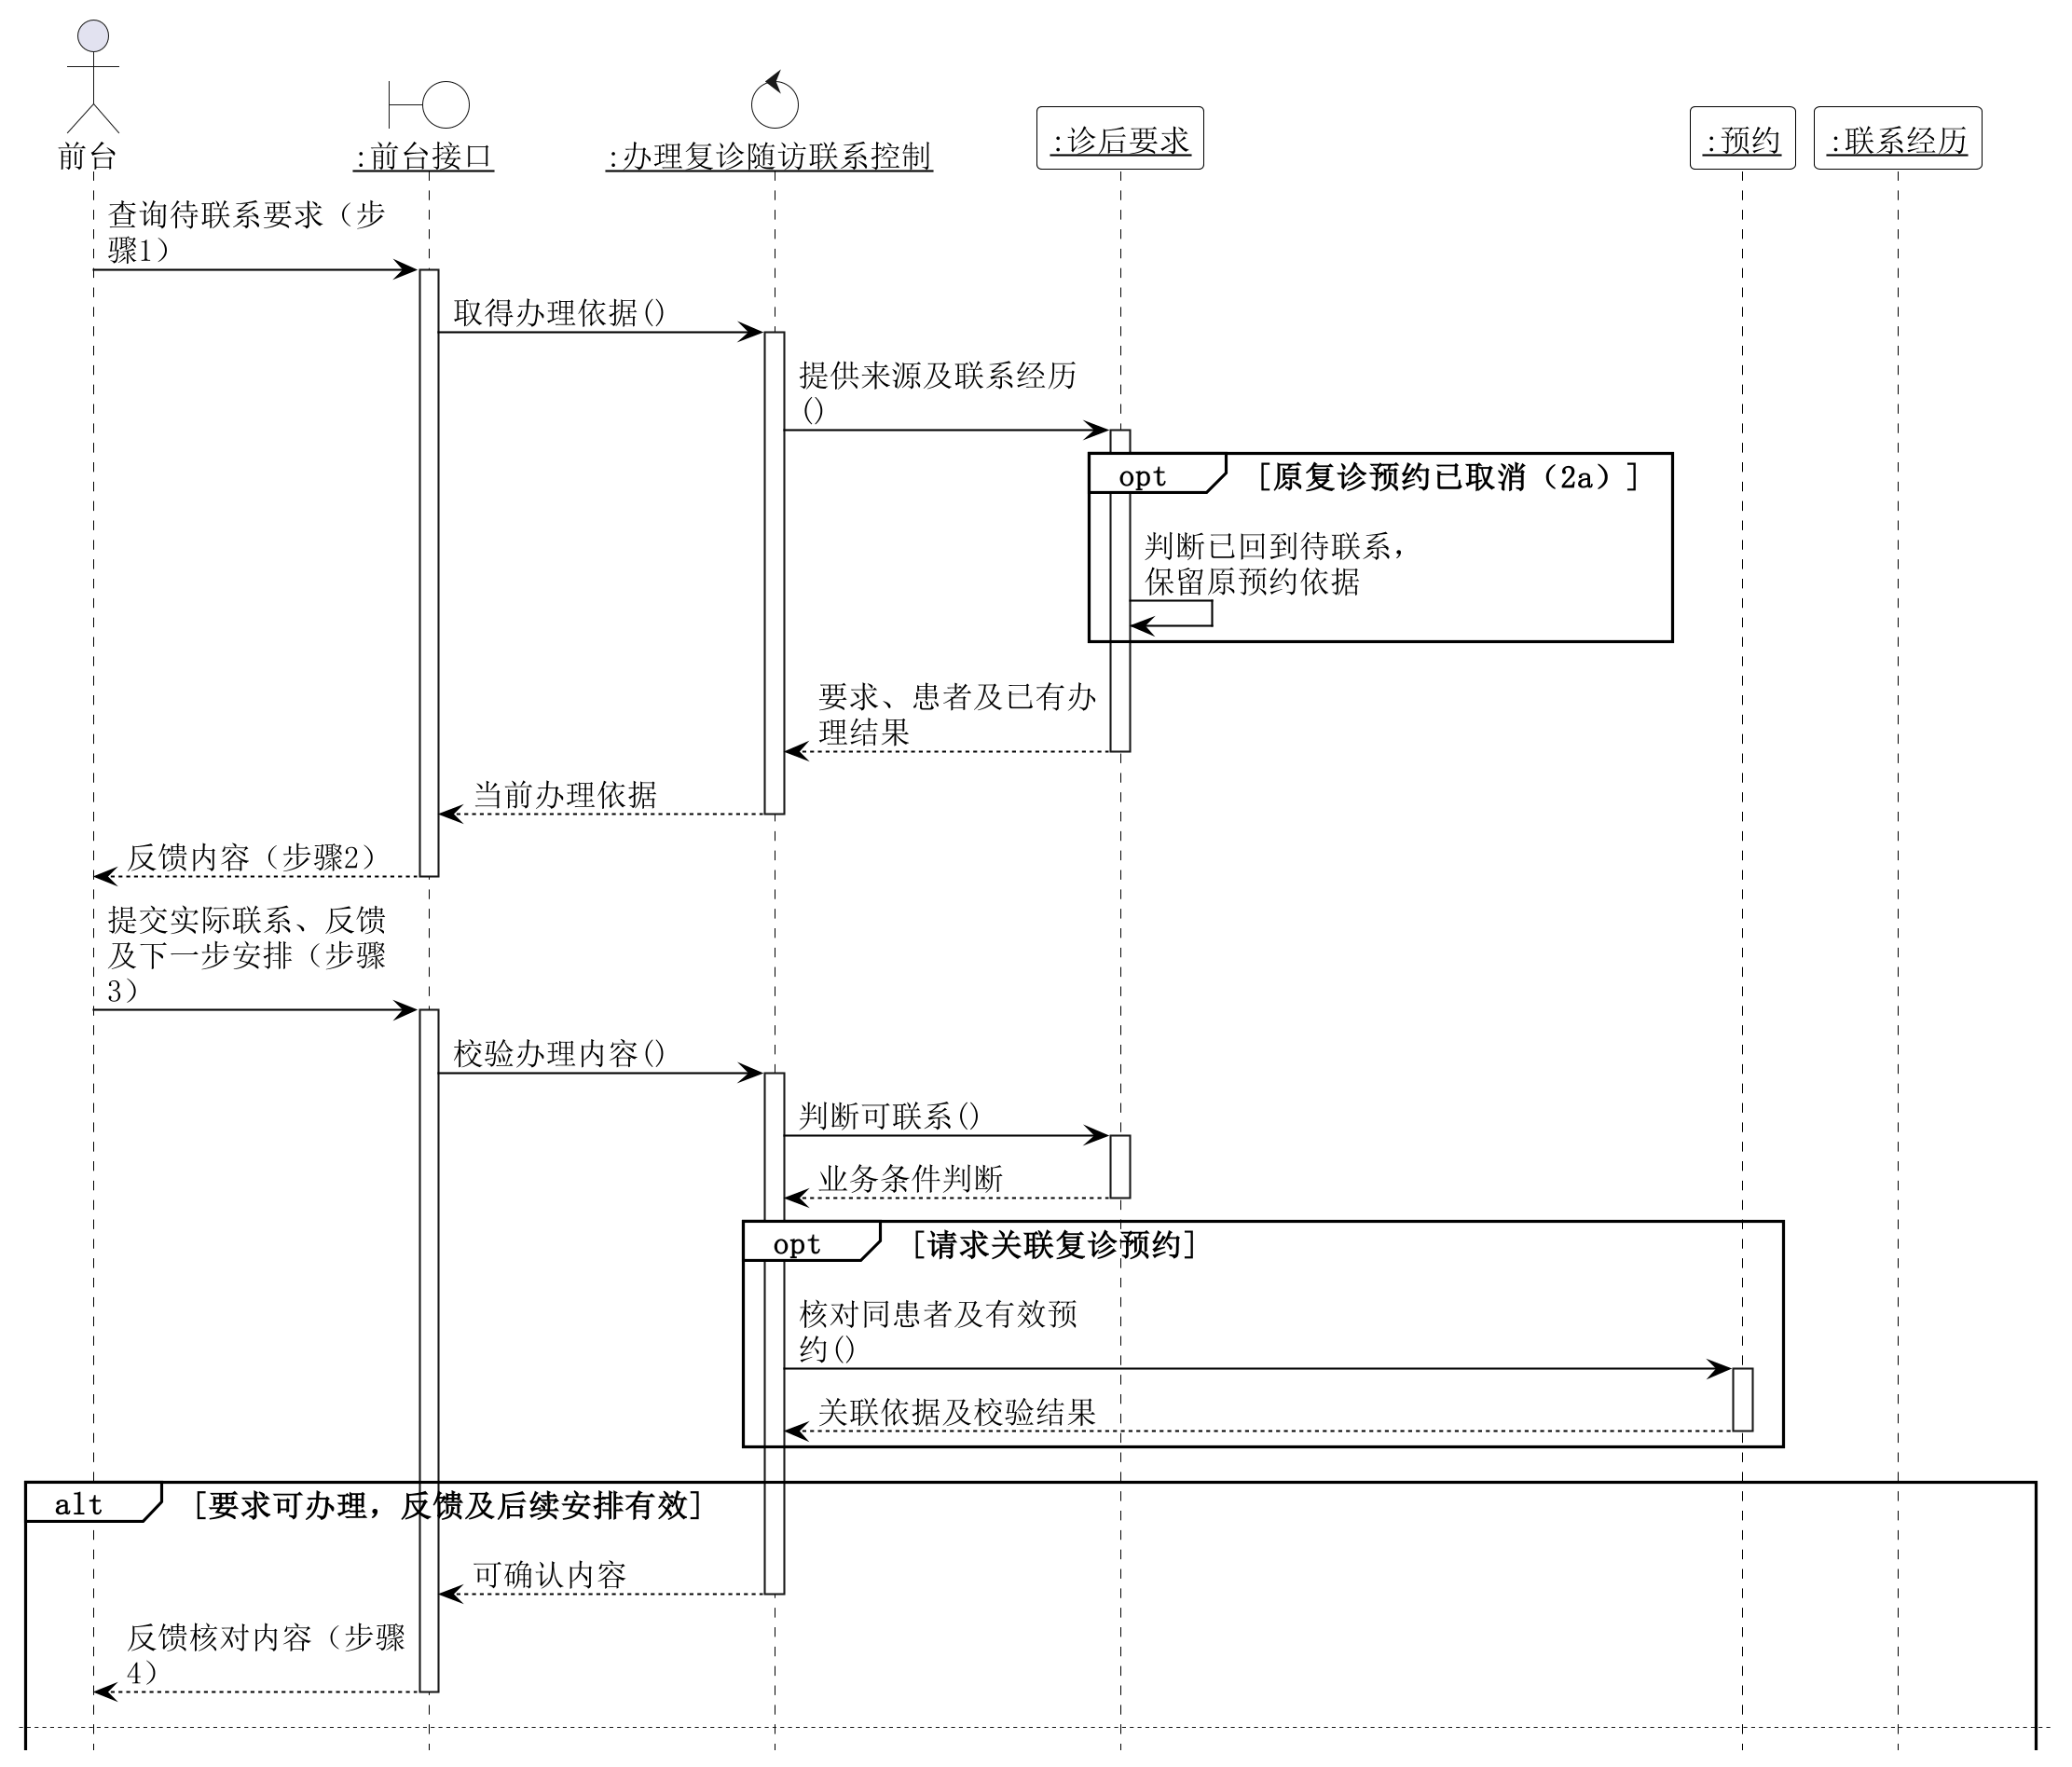
\includegraphics[width=\textwidth,height=20cm,keepaspectratio]{diagrams/13-13-analysis-sequence.png}
\caption{UC-13 办理复诊随访联系分析序列图}
\label{fig:seq-13}
\end{figure}
\clearpage
\noindent\textbf{UC-13 分析序列图（续）}
\begin{figure}[!htbp]
\centering
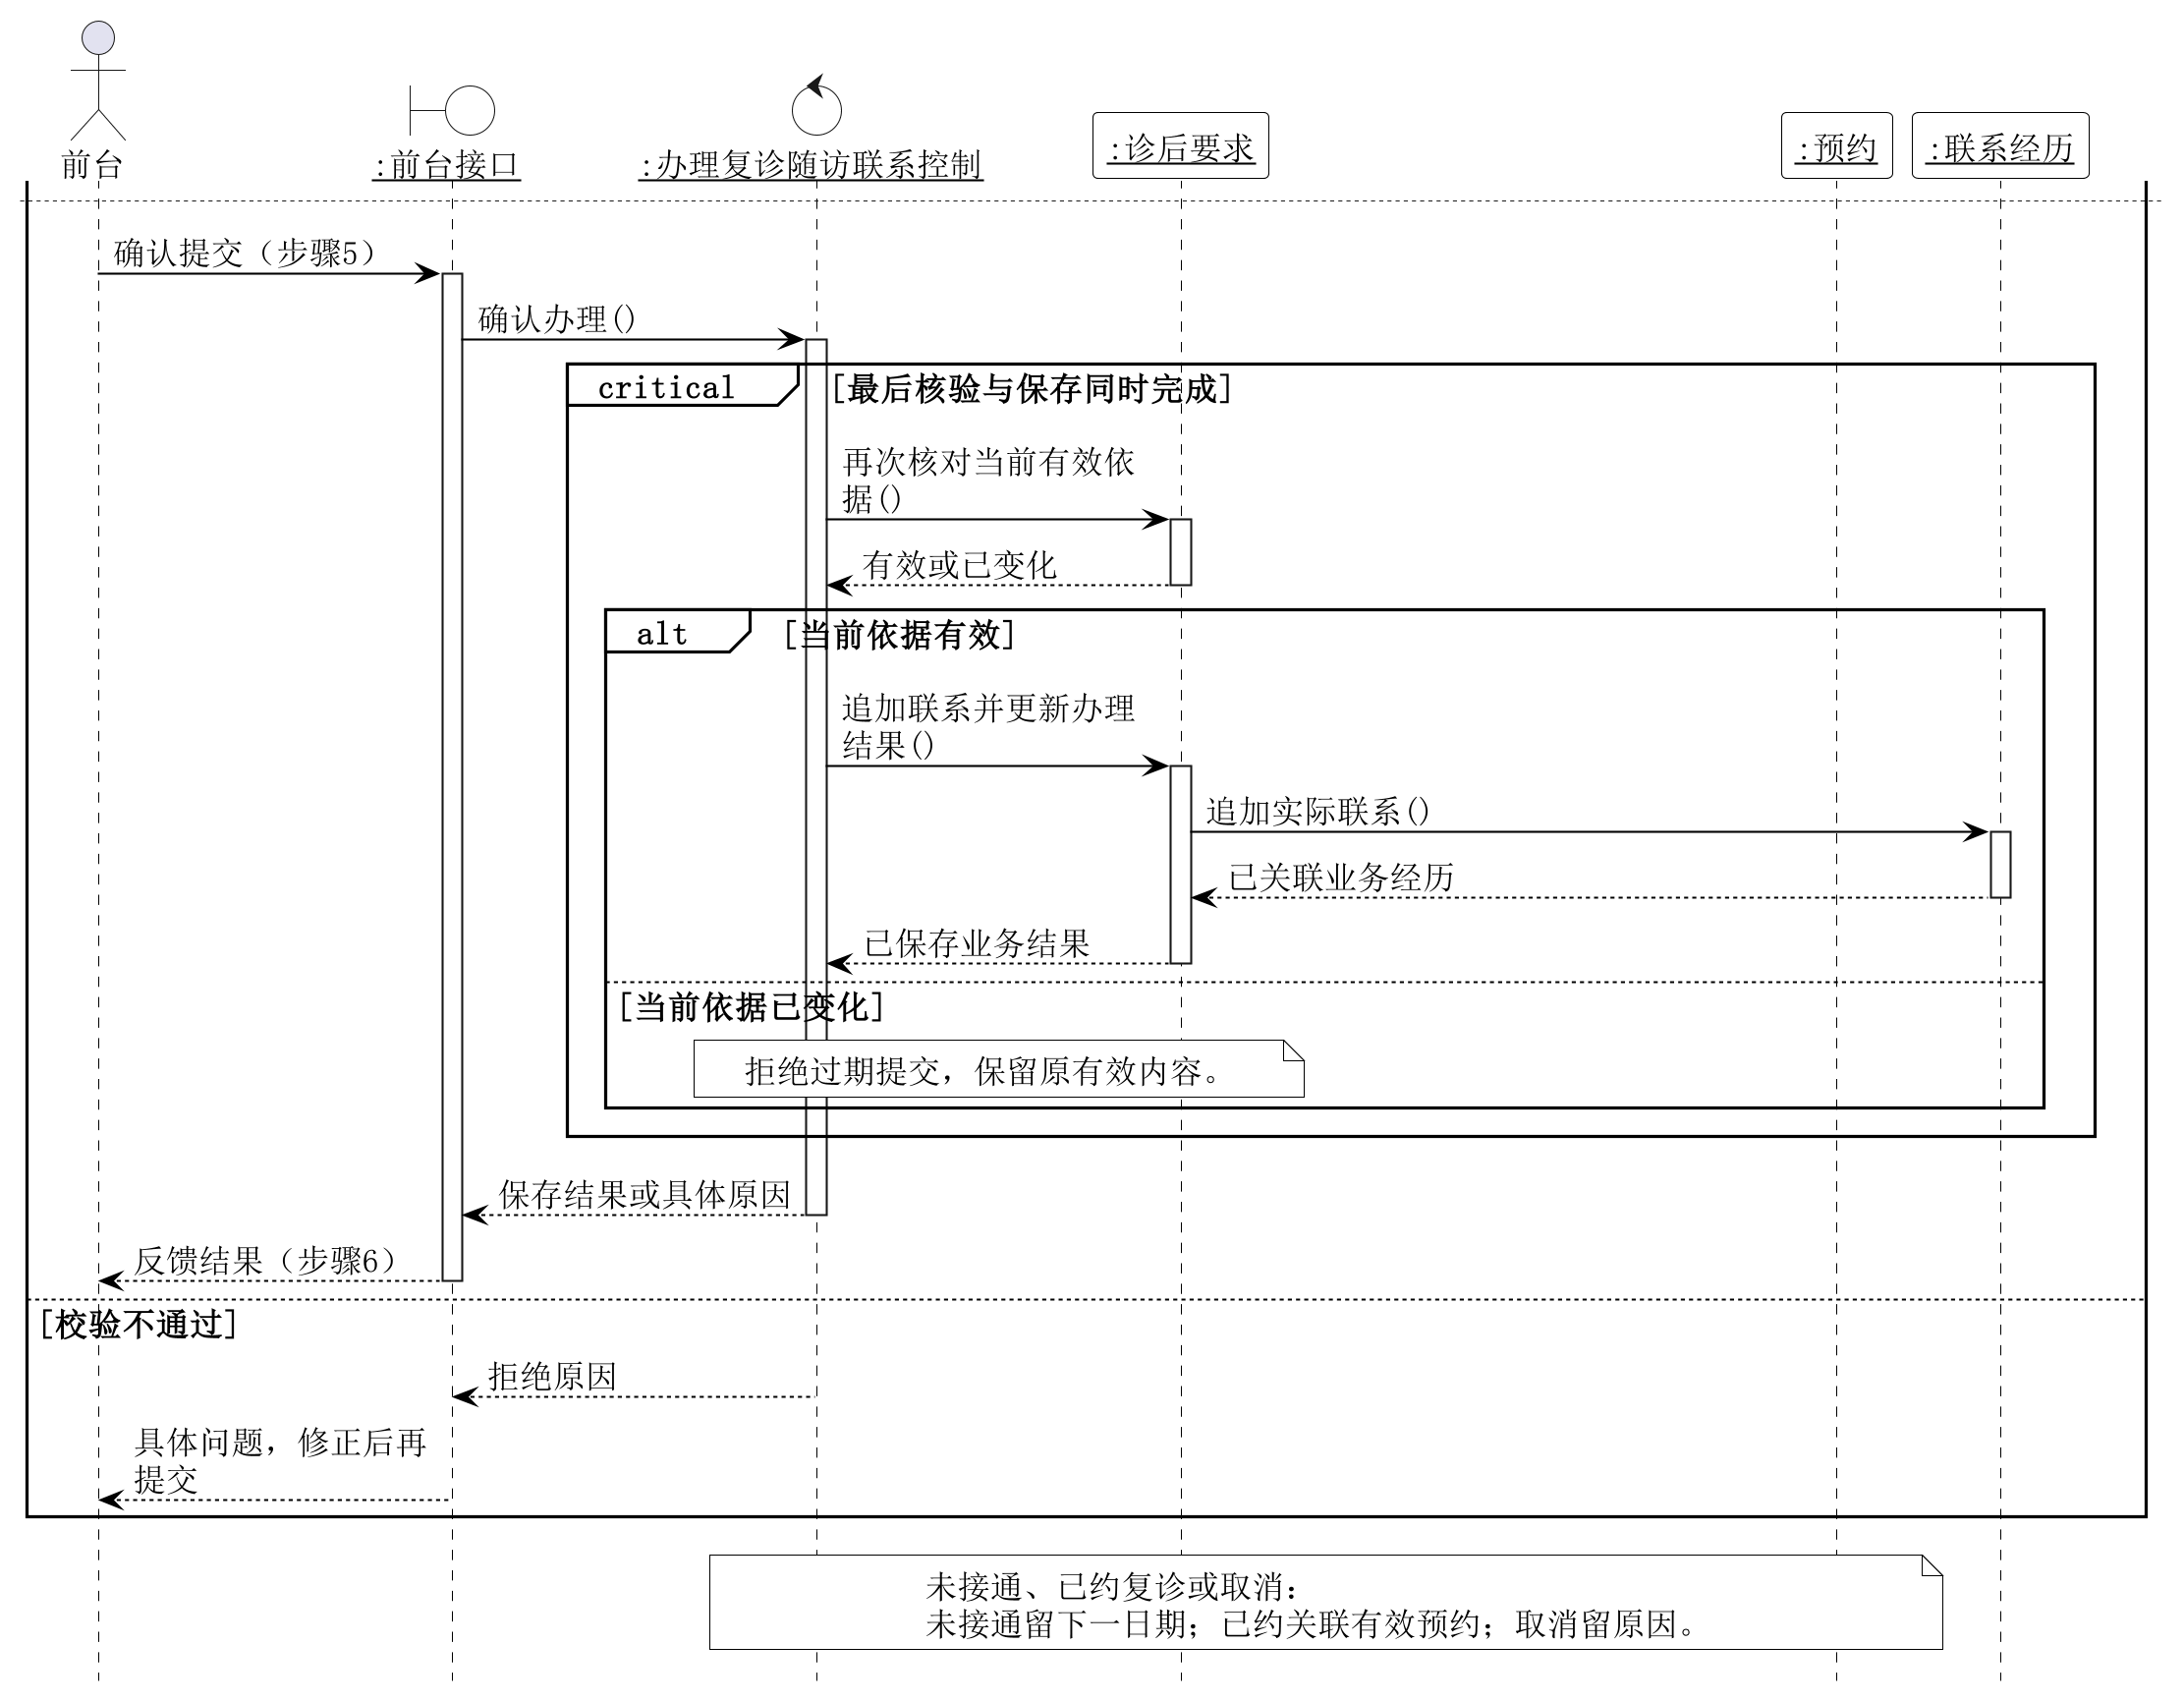
\includegraphics[width=\textwidth,height=20.4cm,keepaspectratio]{diagrams/13-13-analysis-sequence_001.png}
{\normalsize 图\ref{fig:seq-13}（续）：确认与保存}
\end{figure}
\clearpage
\subsubsection{UC-14：记录复诊随访评估}

本图按规约分配诊后要求、临床评估、预约、就诊、病历的业务责任。
\begin{figure}[!htbp]
\centering
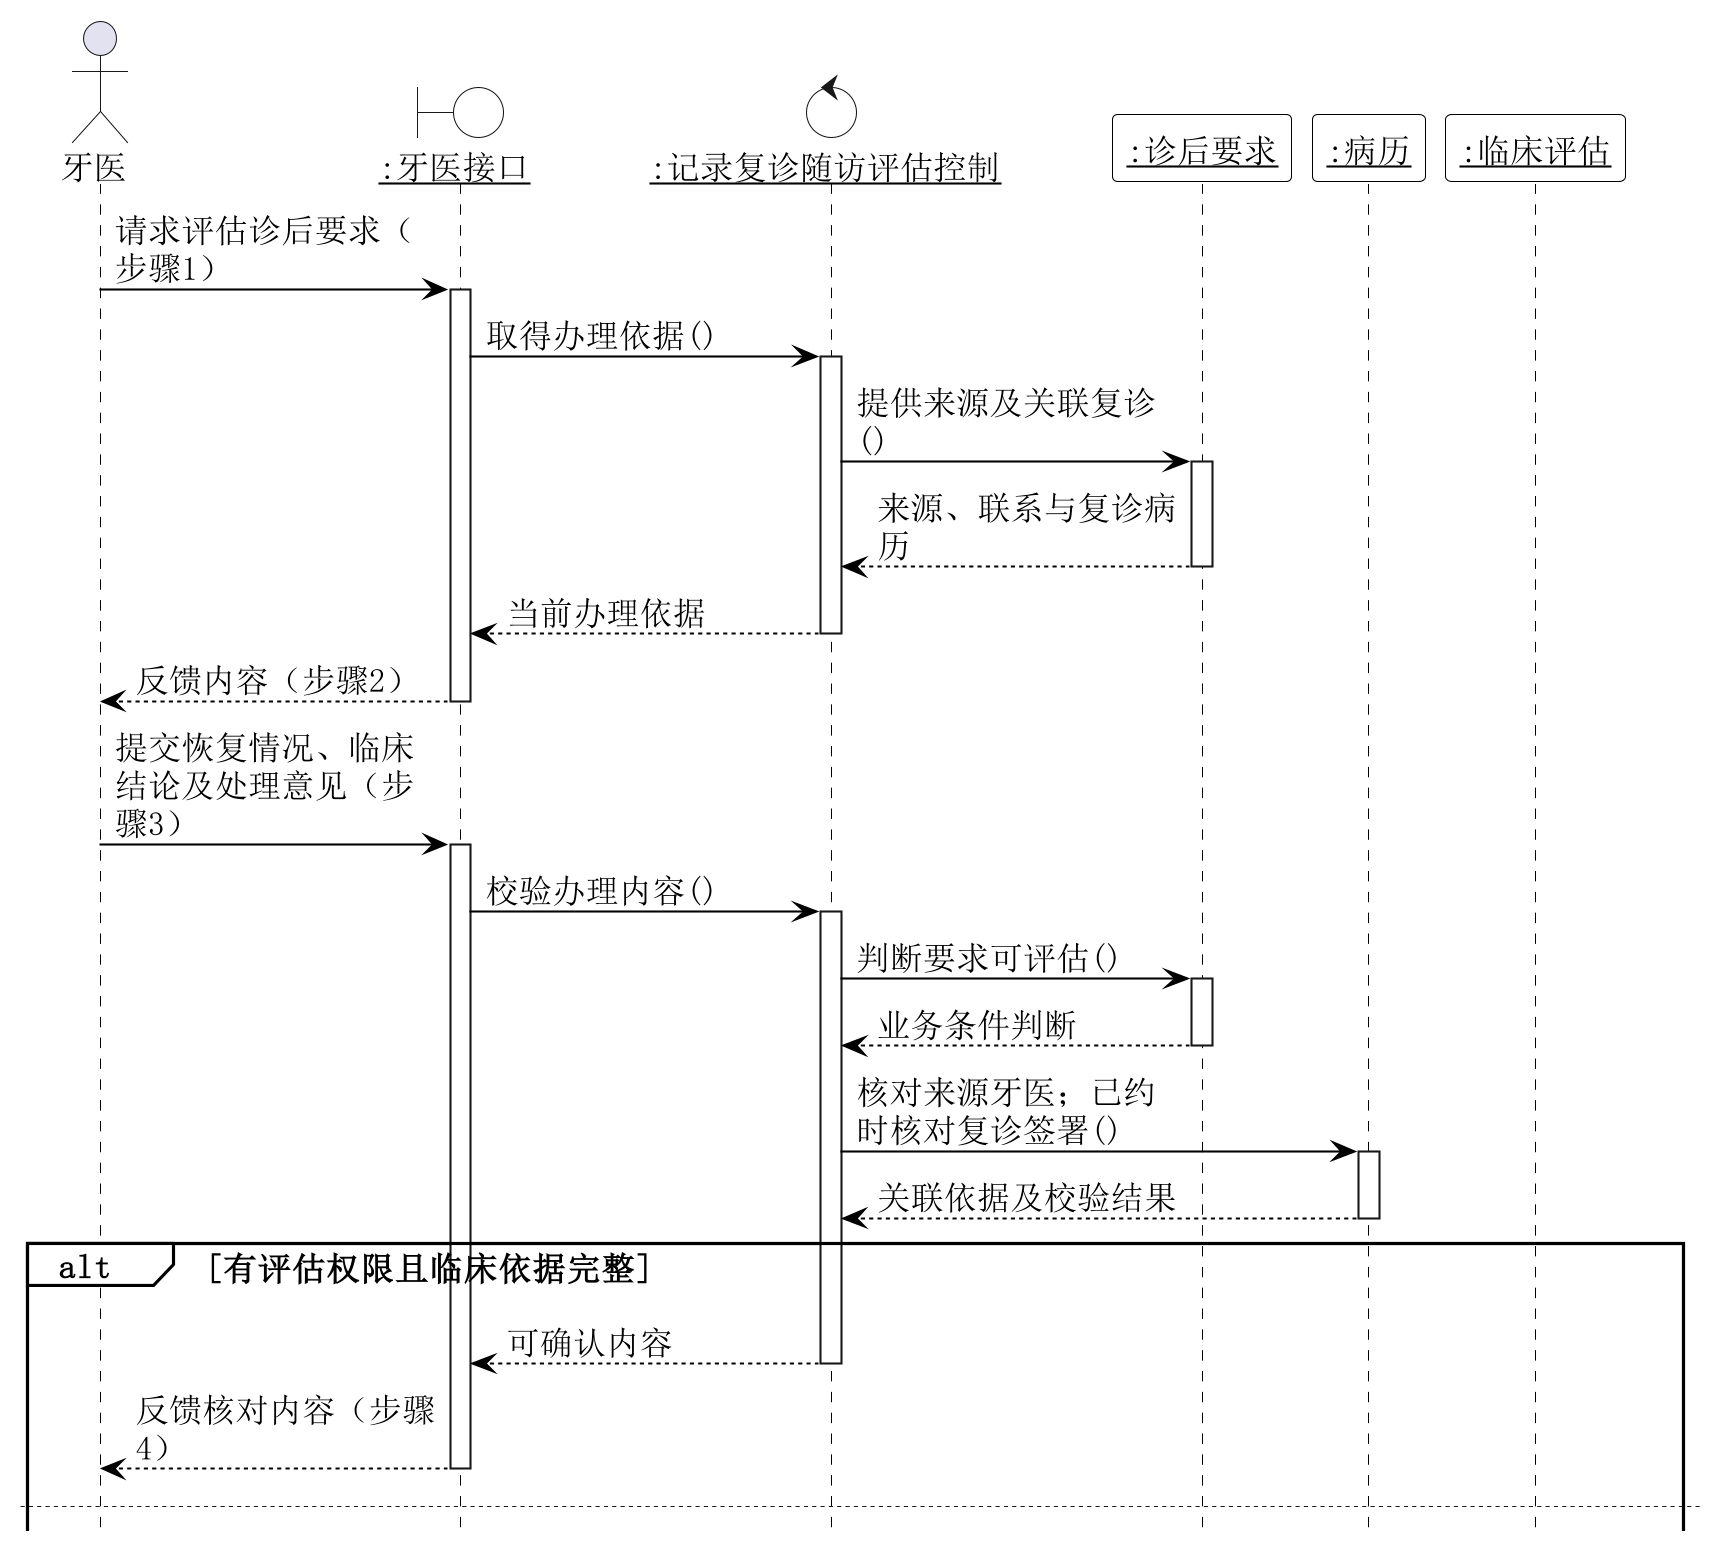
\includegraphics[width=\textwidth,height=20cm,keepaspectratio]{diagrams/13-14-analysis-sequence.png}
\caption{UC-14 记录复诊随访评估分析序列图}
\label{fig:seq-14}
\end{figure}
\clearpage
\noindent\textbf{UC-14 分析序列图（续）}
\begin{figure}[!htbp]
\centering
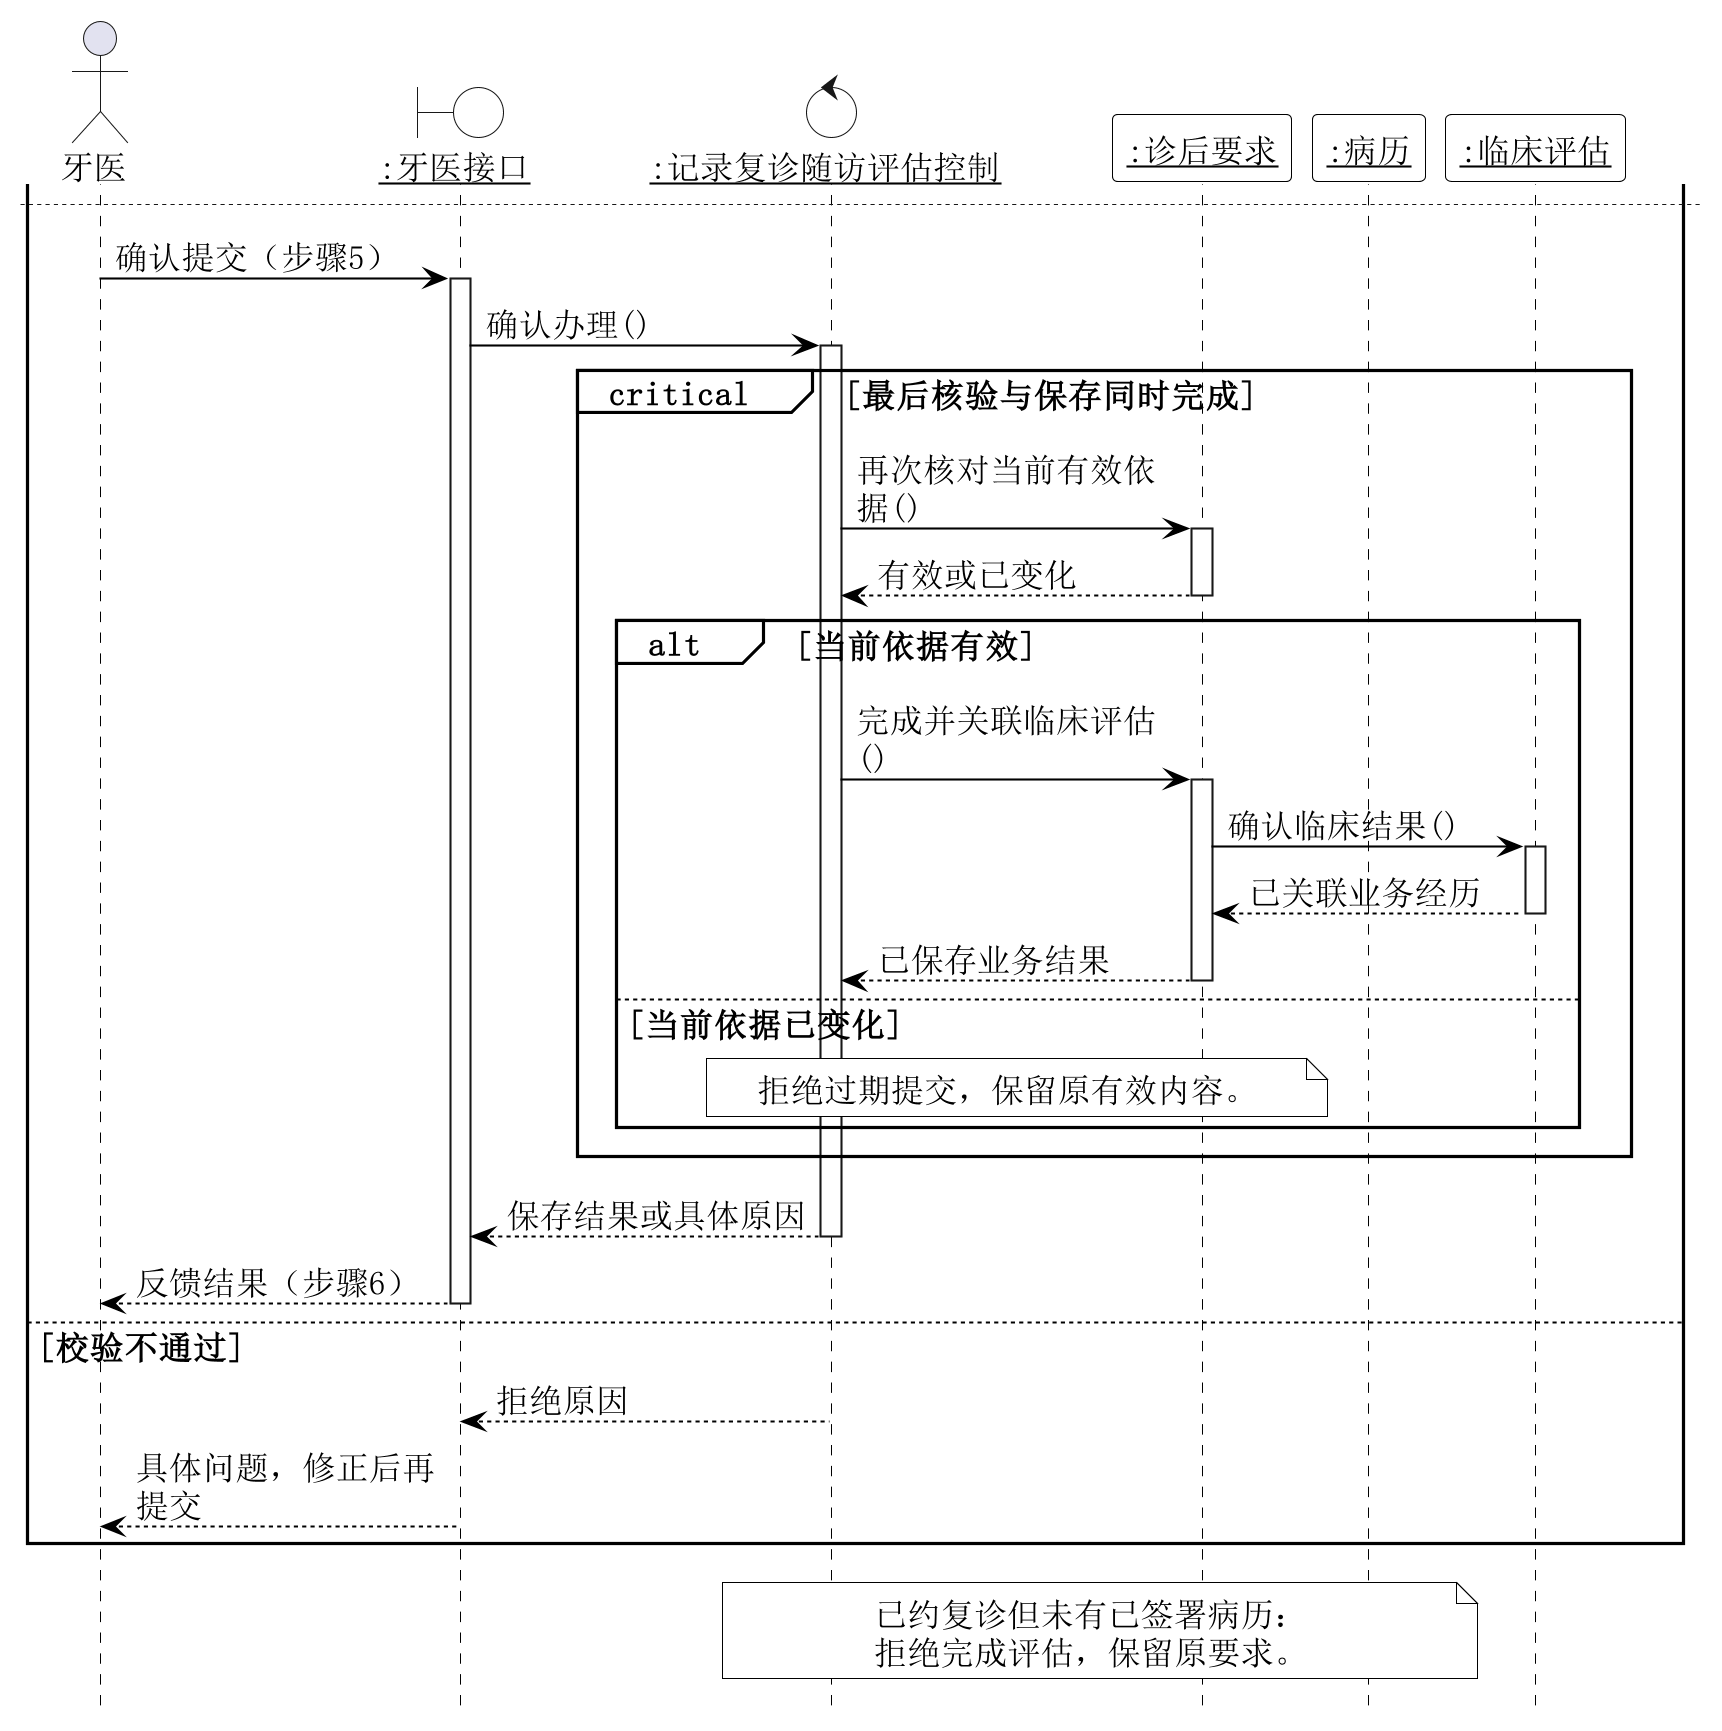
\includegraphics[width=\textwidth,height=20.4cm,keepaspectratio]{diagrams/13-14-analysis-sequence_001.png}
{\normalsize 图\ref{fig:seq-14}（续）：确认与保存}
\end{figure}
\clearpage
\subsubsection{UC-15：维护接诊人员安排}

本图按规约分配职员、接诊时段、预约的业务责任。
\begin{figure}[!htbp]
\centering
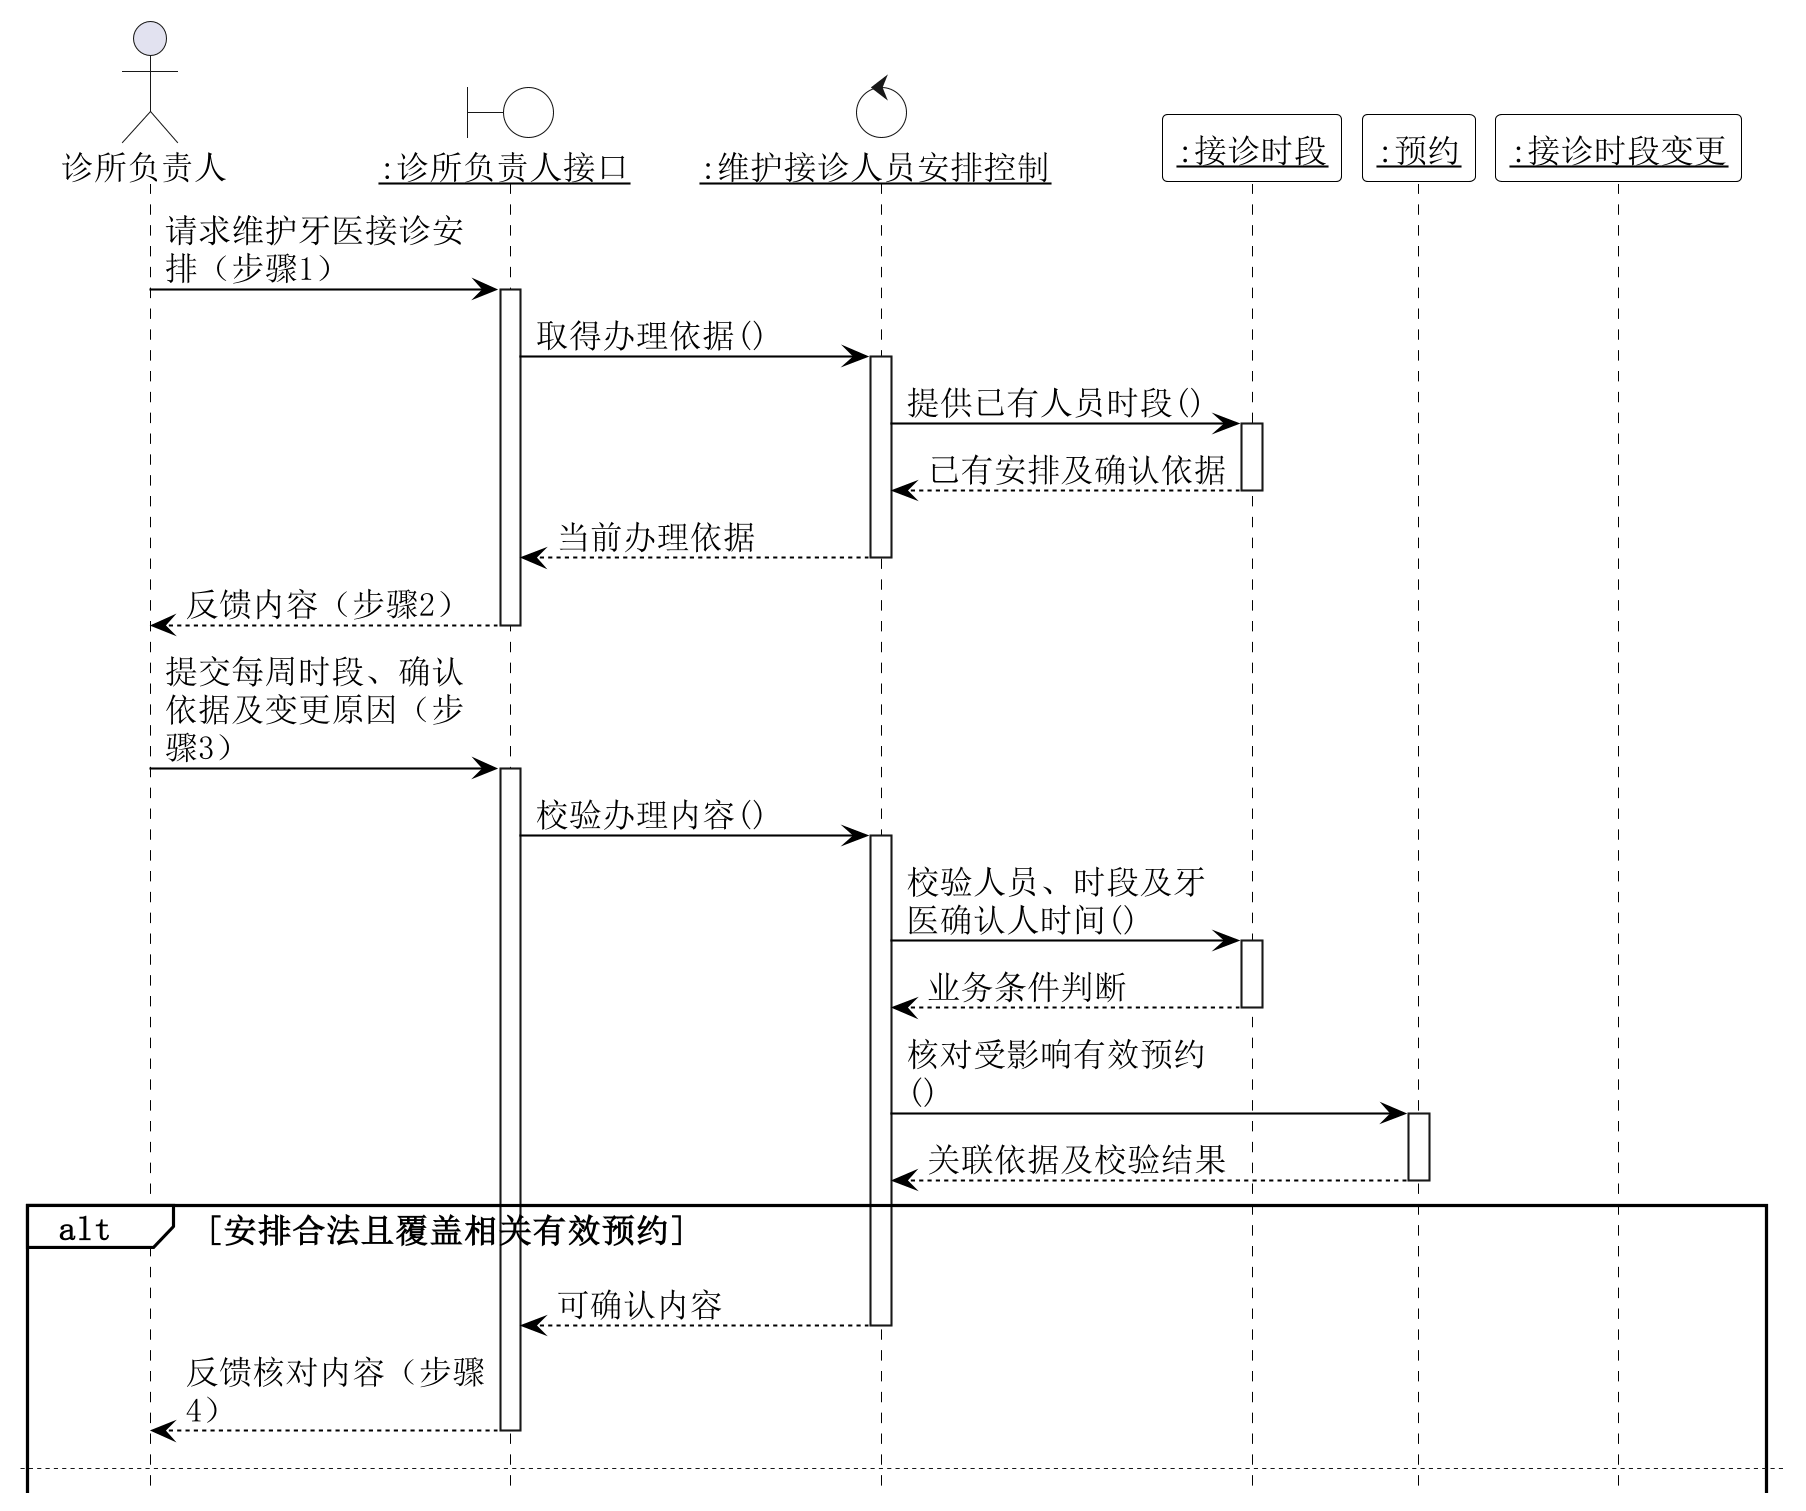
\includegraphics[width=\textwidth,height=20cm,keepaspectratio]{diagrams/13-15-analysis-sequence.png}
\caption{UC-15 维护接诊人员安排分析序列图}
\label{fig:seq-15}
\end{figure}
\clearpage
\noindent\textbf{UC-15 分析序列图（续）}
\begin{figure}[!htbp]
\centering
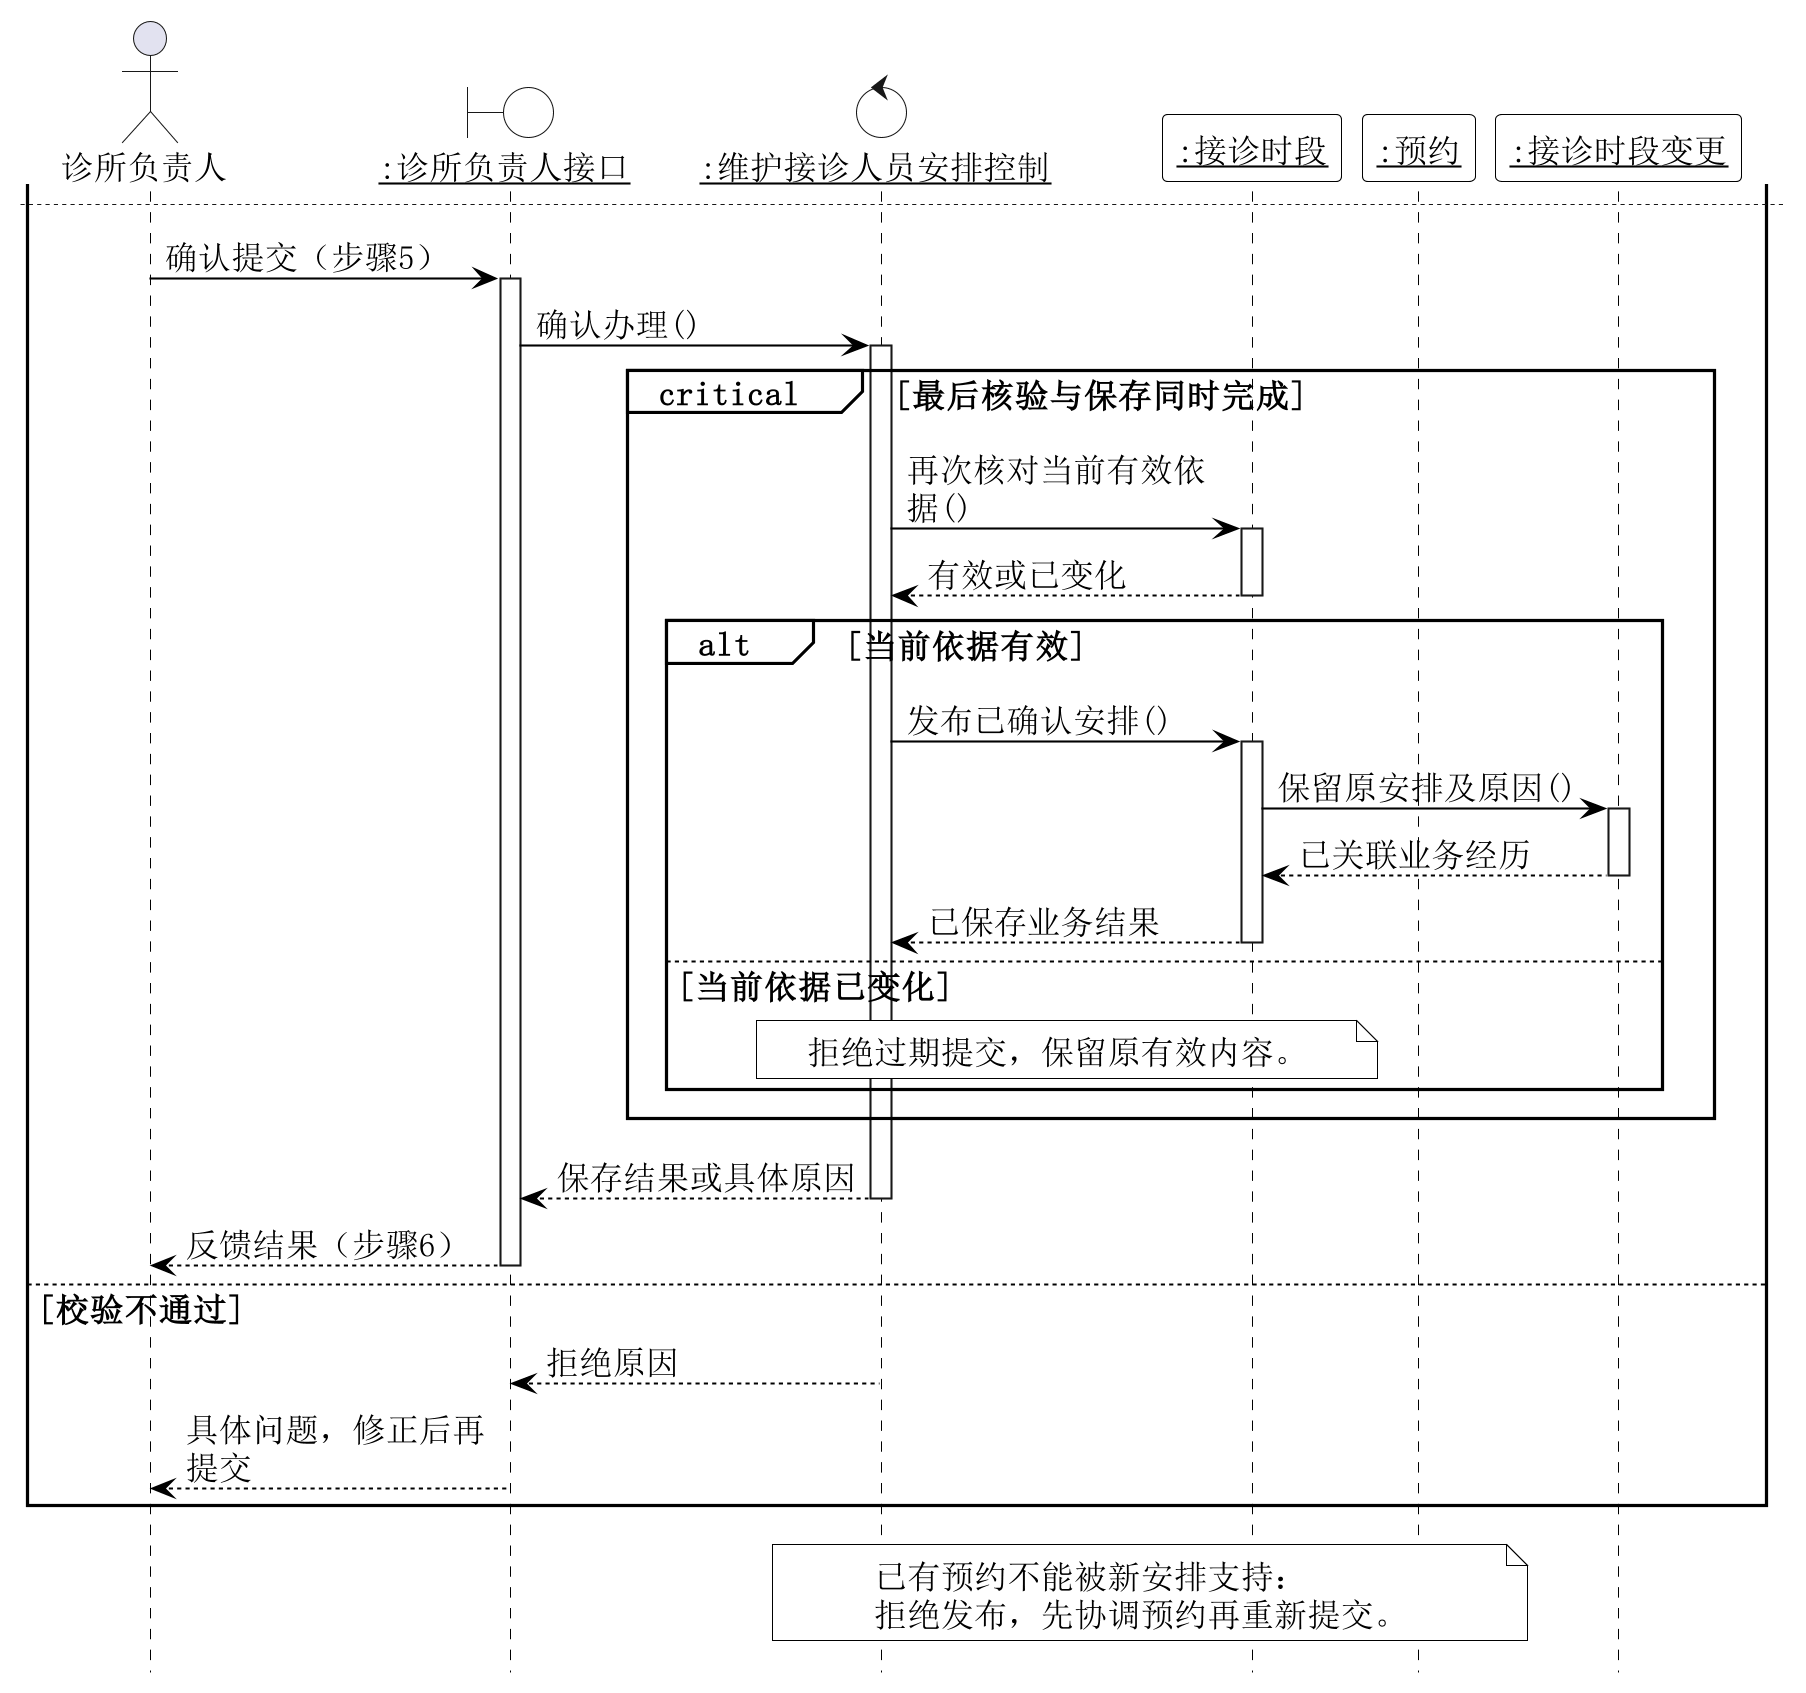
\includegraphics[width=\textwidth,height=20.4cm,keepaspectratio]{diagrams/13-15-analysis-sequence_001.png}
{\normalsize 图\ref{fig:seq-15}（续）：确认与保存}
\end{figure}
\clearpage
\subsubsection{UC-16：查询可用接诊安排}

本图按规约分配职员、接诊时段、预约的业务责任。
\begin{figure}[!htbp]
\centering
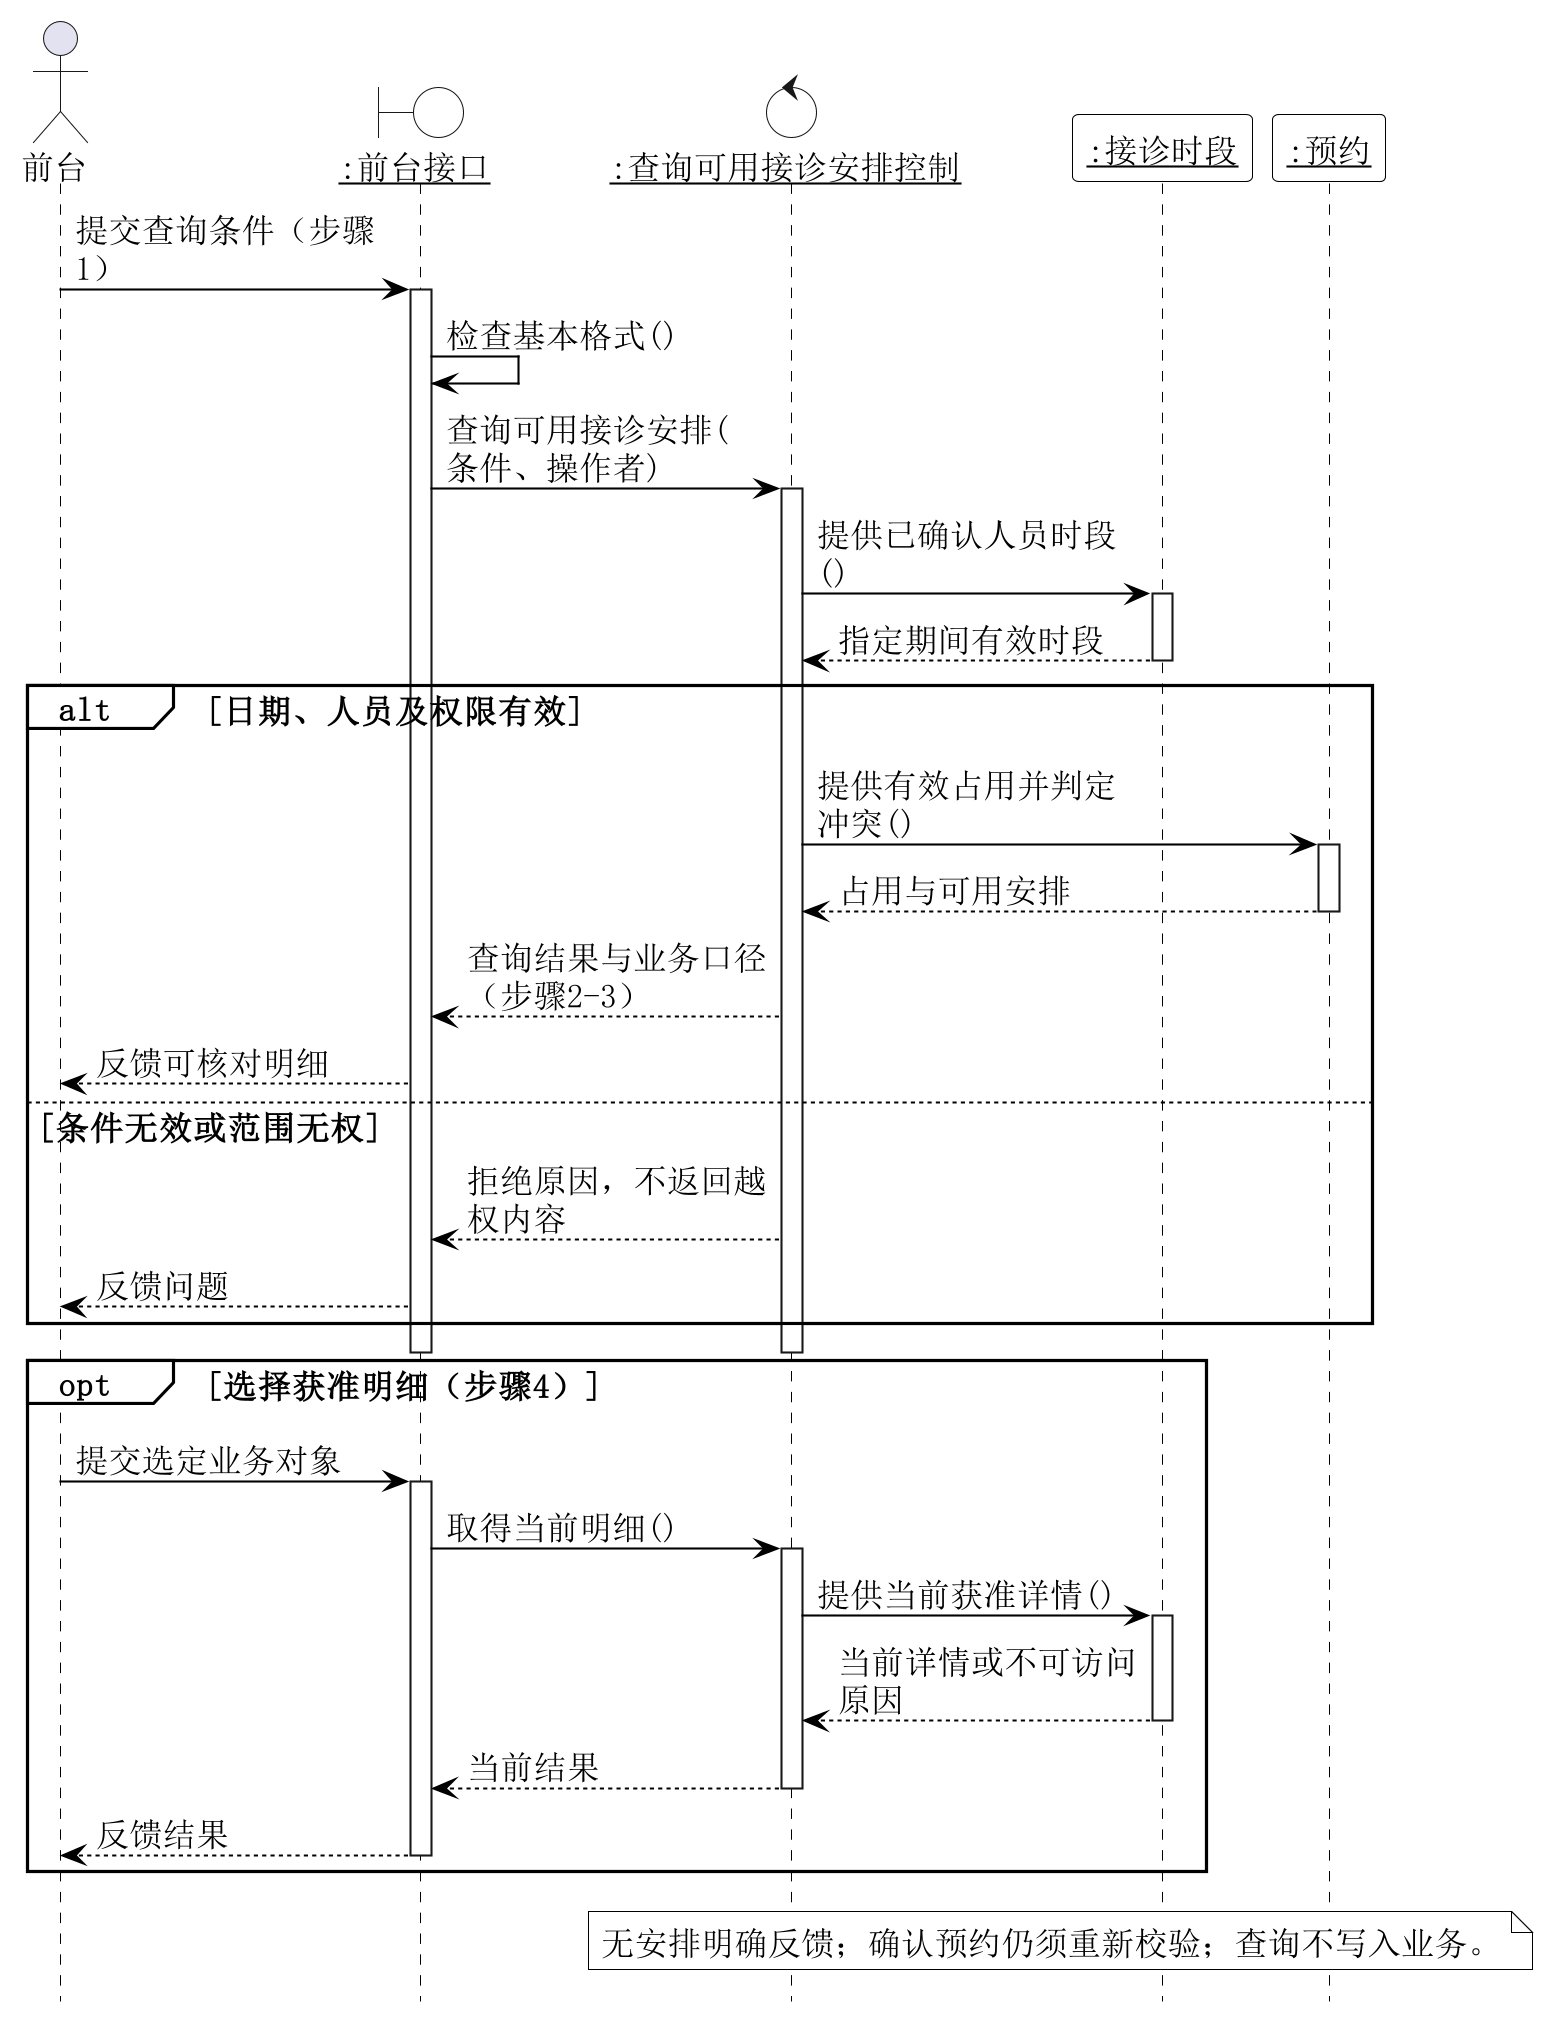
\includegraphics[width=\textwidth,height=20cm,keepaspectratio]{diagrams/13-16-analysis-sequence.png}
\caption{UC-16 查询可用接诊安排分析序列图}
\label{fig:seq-16}
\end{figure}
\clearpage
\begin{figure}[!htbp]
\centering
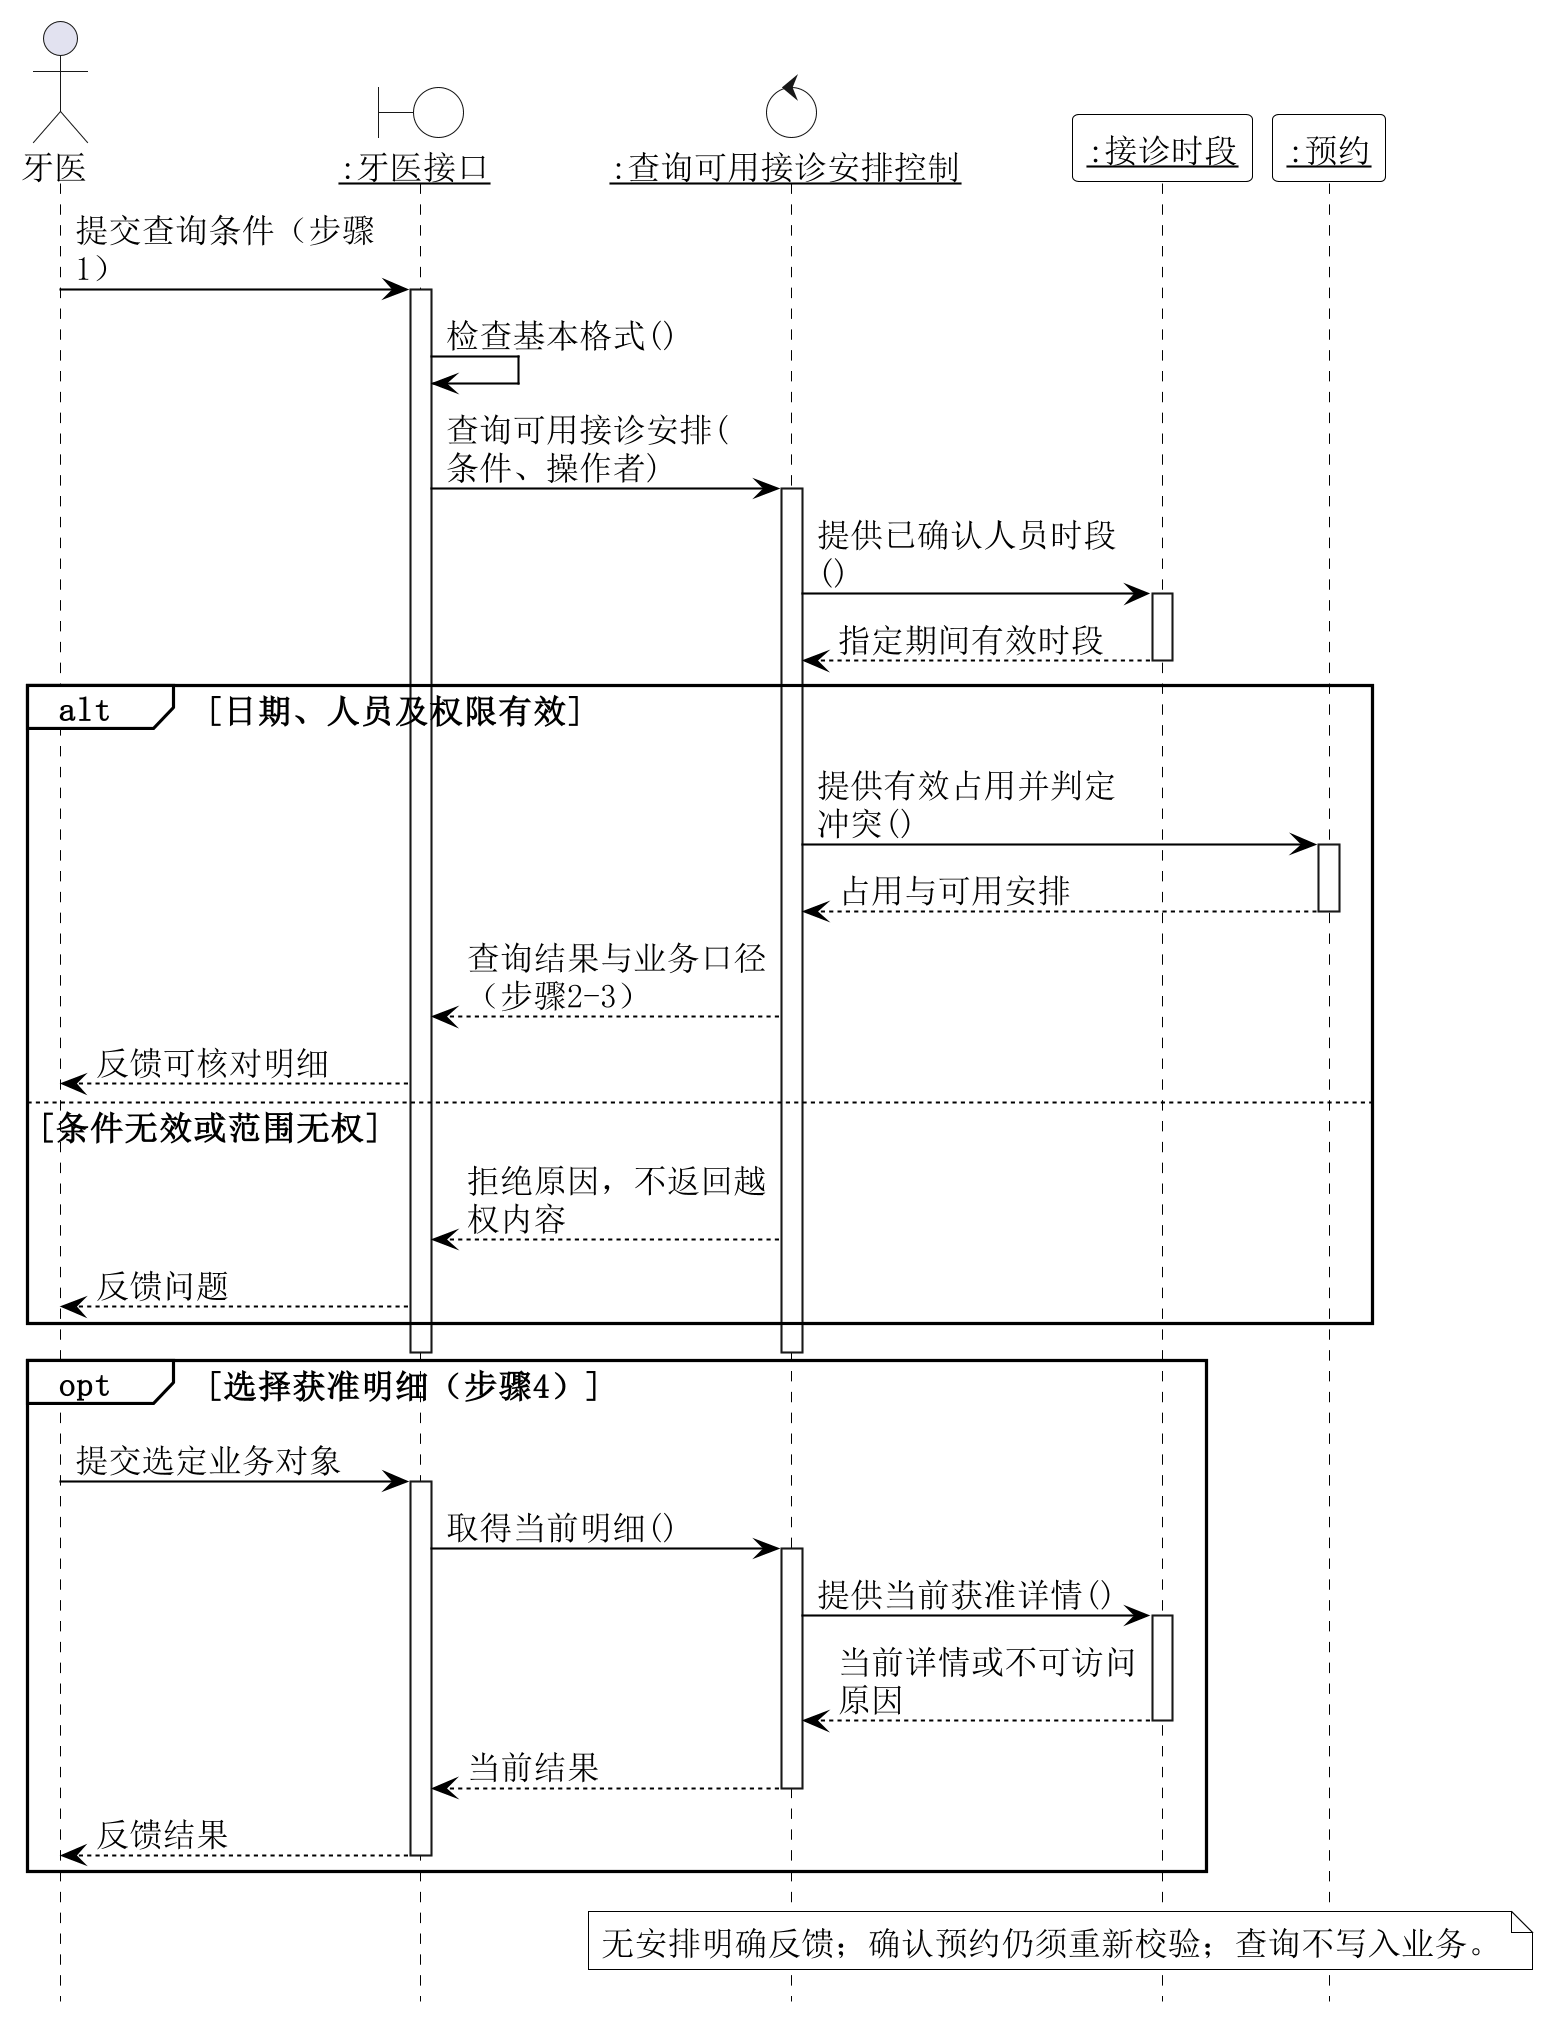
\includegraphics[width=\textwidth,height=20cm,keepaspectratio]{diagrams/13-16-alt-analysis-sequence.png}
\caption{UC-16 牙医查询分析序列图}
\label{fig:seq-16-alt}
\end{figure}
\clearpage
\subsubsection{UC-17：查询材料库存}

本图按规约分配材料、材料变动、职员的业务责任。
\begin{figure}[!htbp]
\centering
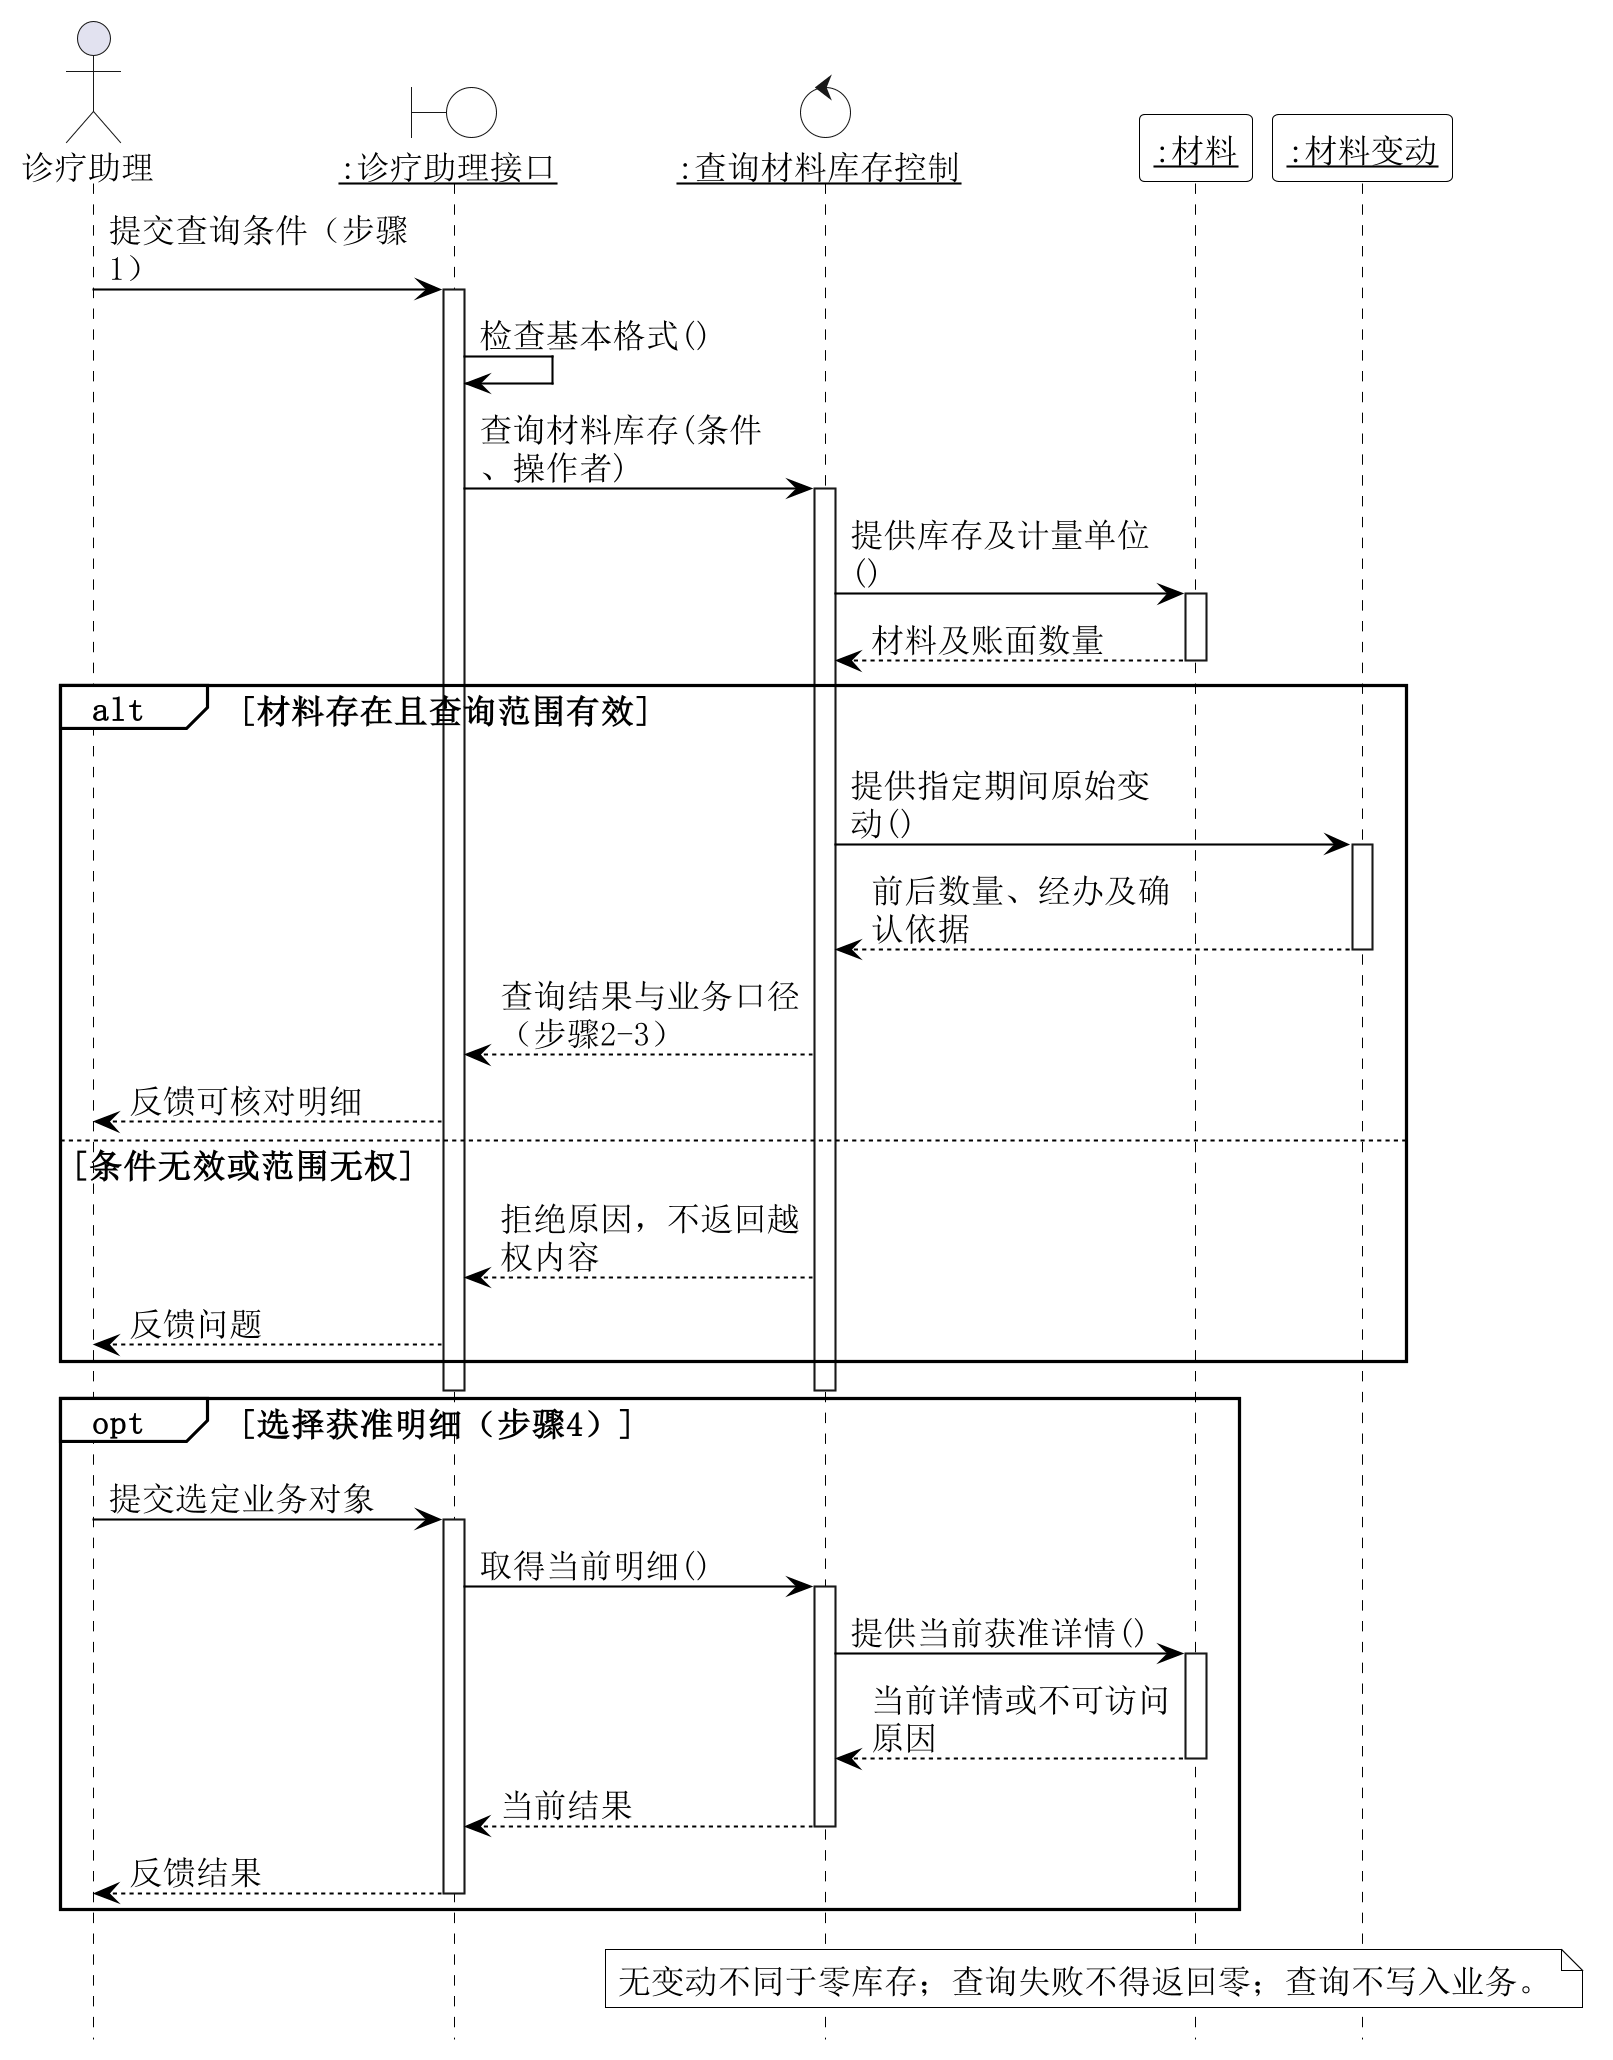
\includegraphics[width=\textwidth,height=20cm,keepaspectratio]{diagrams/13-17-analysis-sequence.png}
\caption{UC-17 查询材料库存分析序列图}
\label{fig:seq-17}
\end{figure}
\clearpage
\begin{figure}[!htbp]
\centering
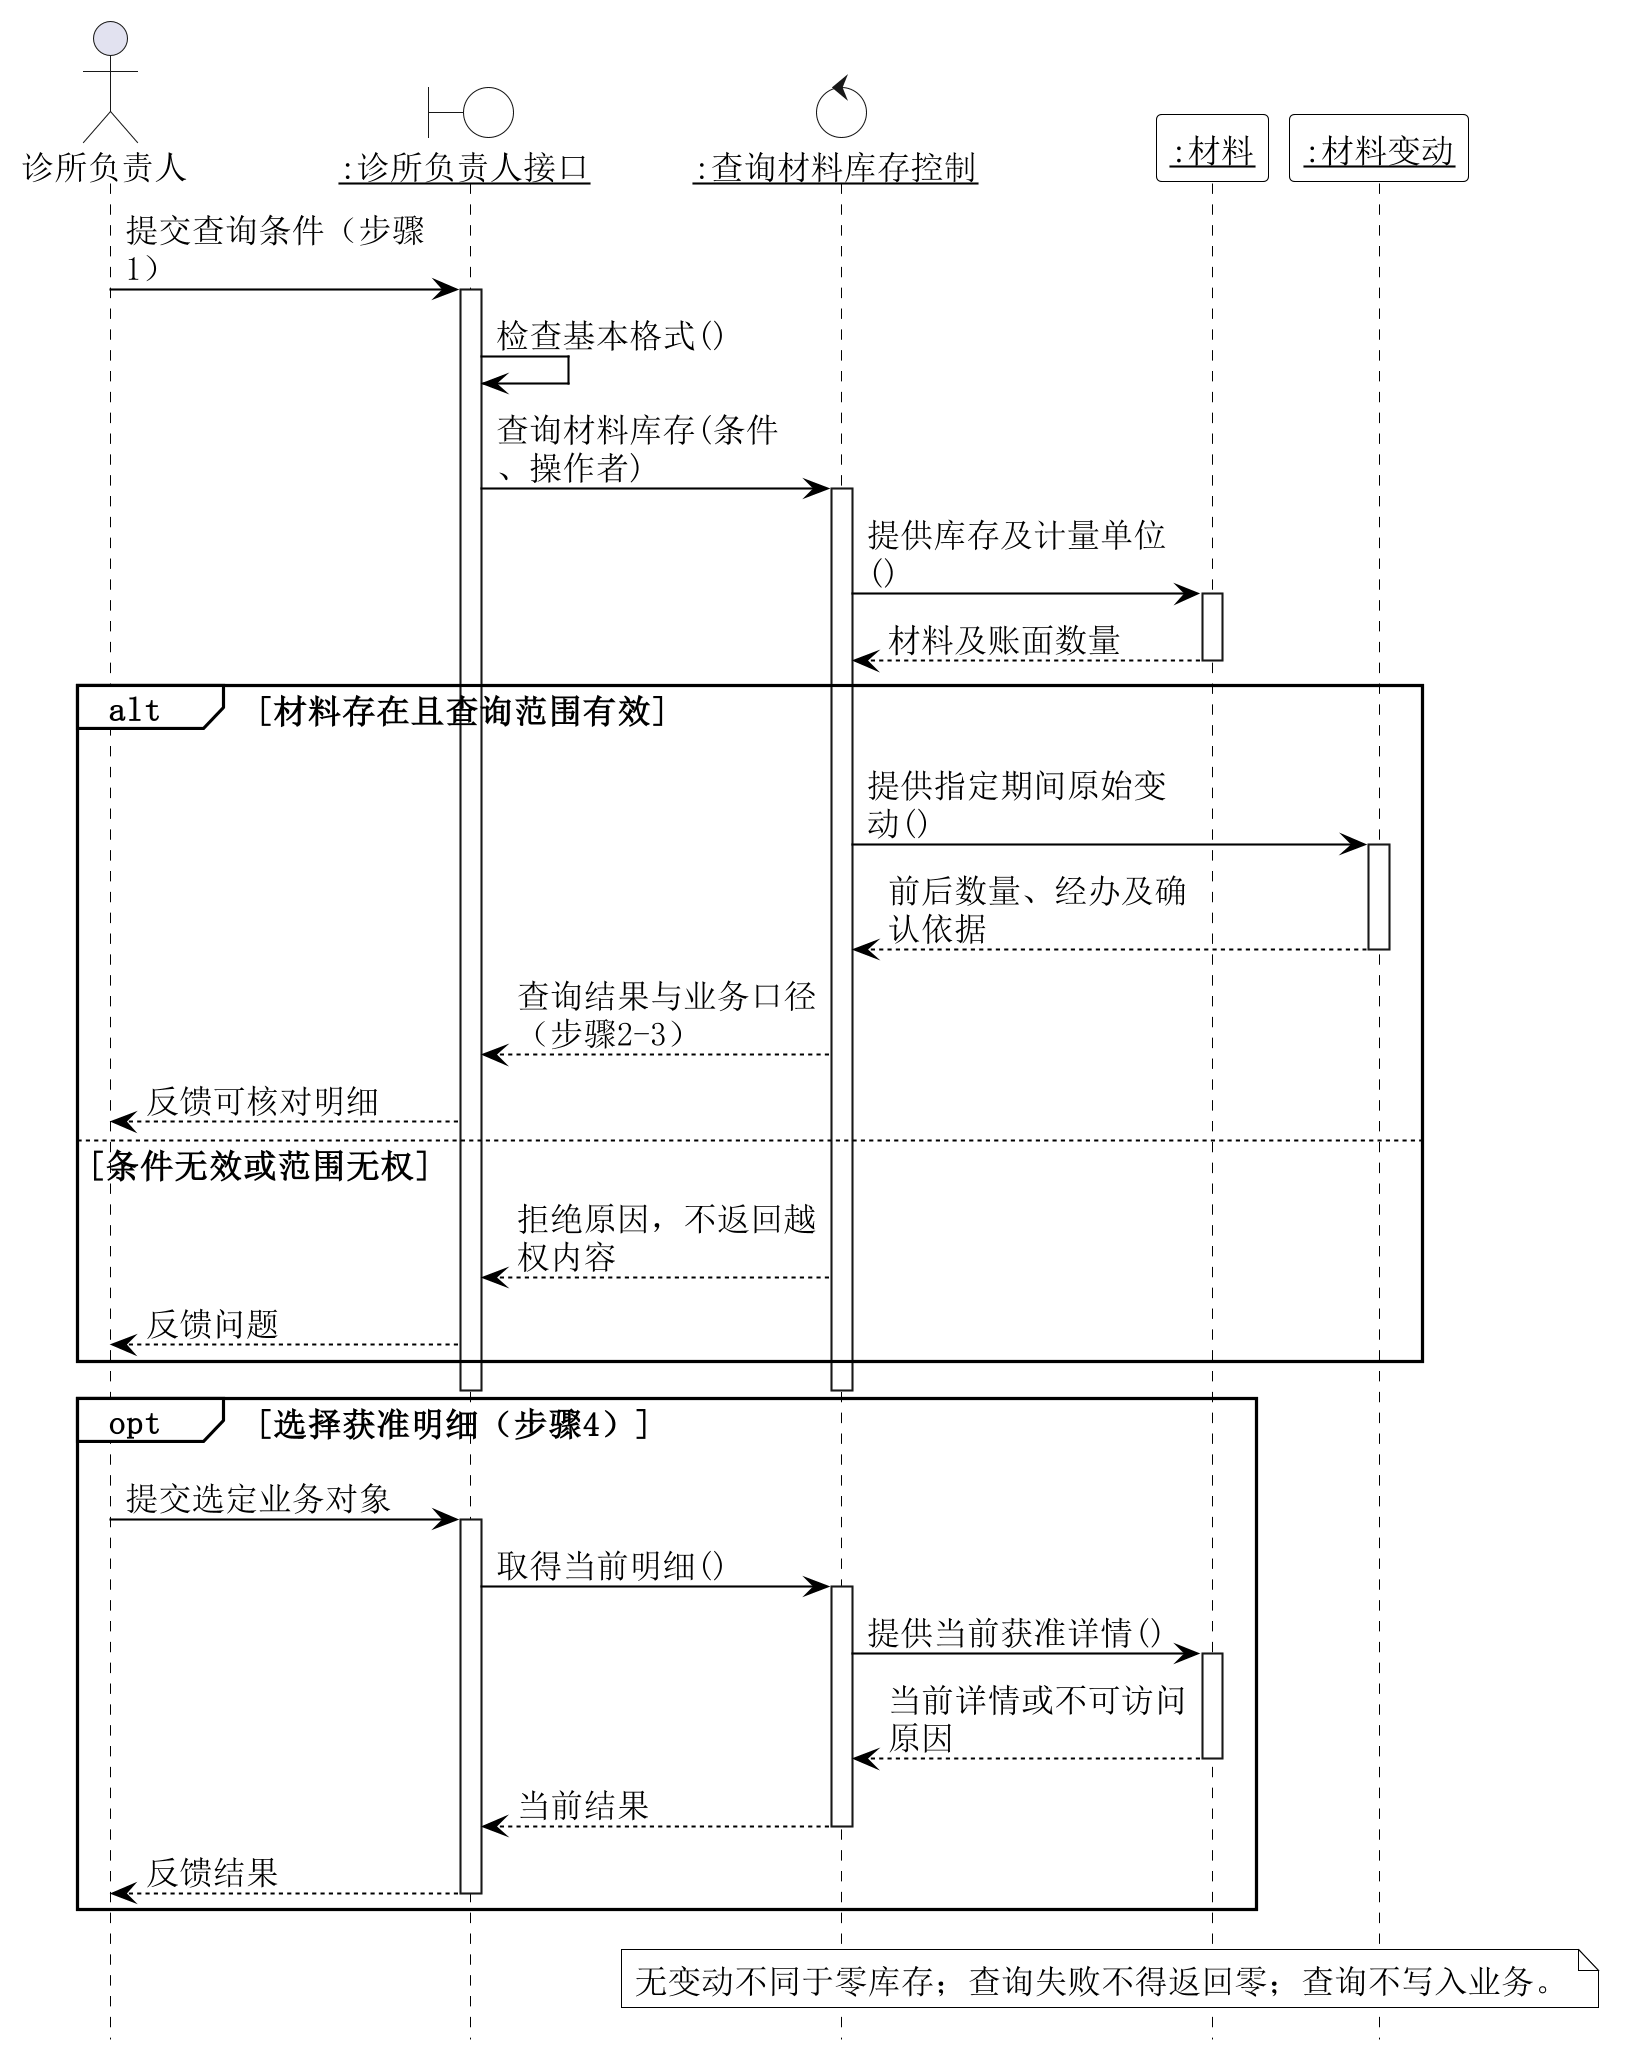
\includegraphics[width=\textwidth,height=20cm,keepaspectratio]{diagrams/13-17-alt-analysis-sequence.png}
\caption{UC-17 诊所负责人查询分析序列图}
\label{fig:seq-17-alt}
\end{figure}
\clearpage
\subsubsection{UC-18：登记材料变动}

本图按规约分配材料、材料变动、职员的业务责任。
\begin{figure}[!htbp]
\centering
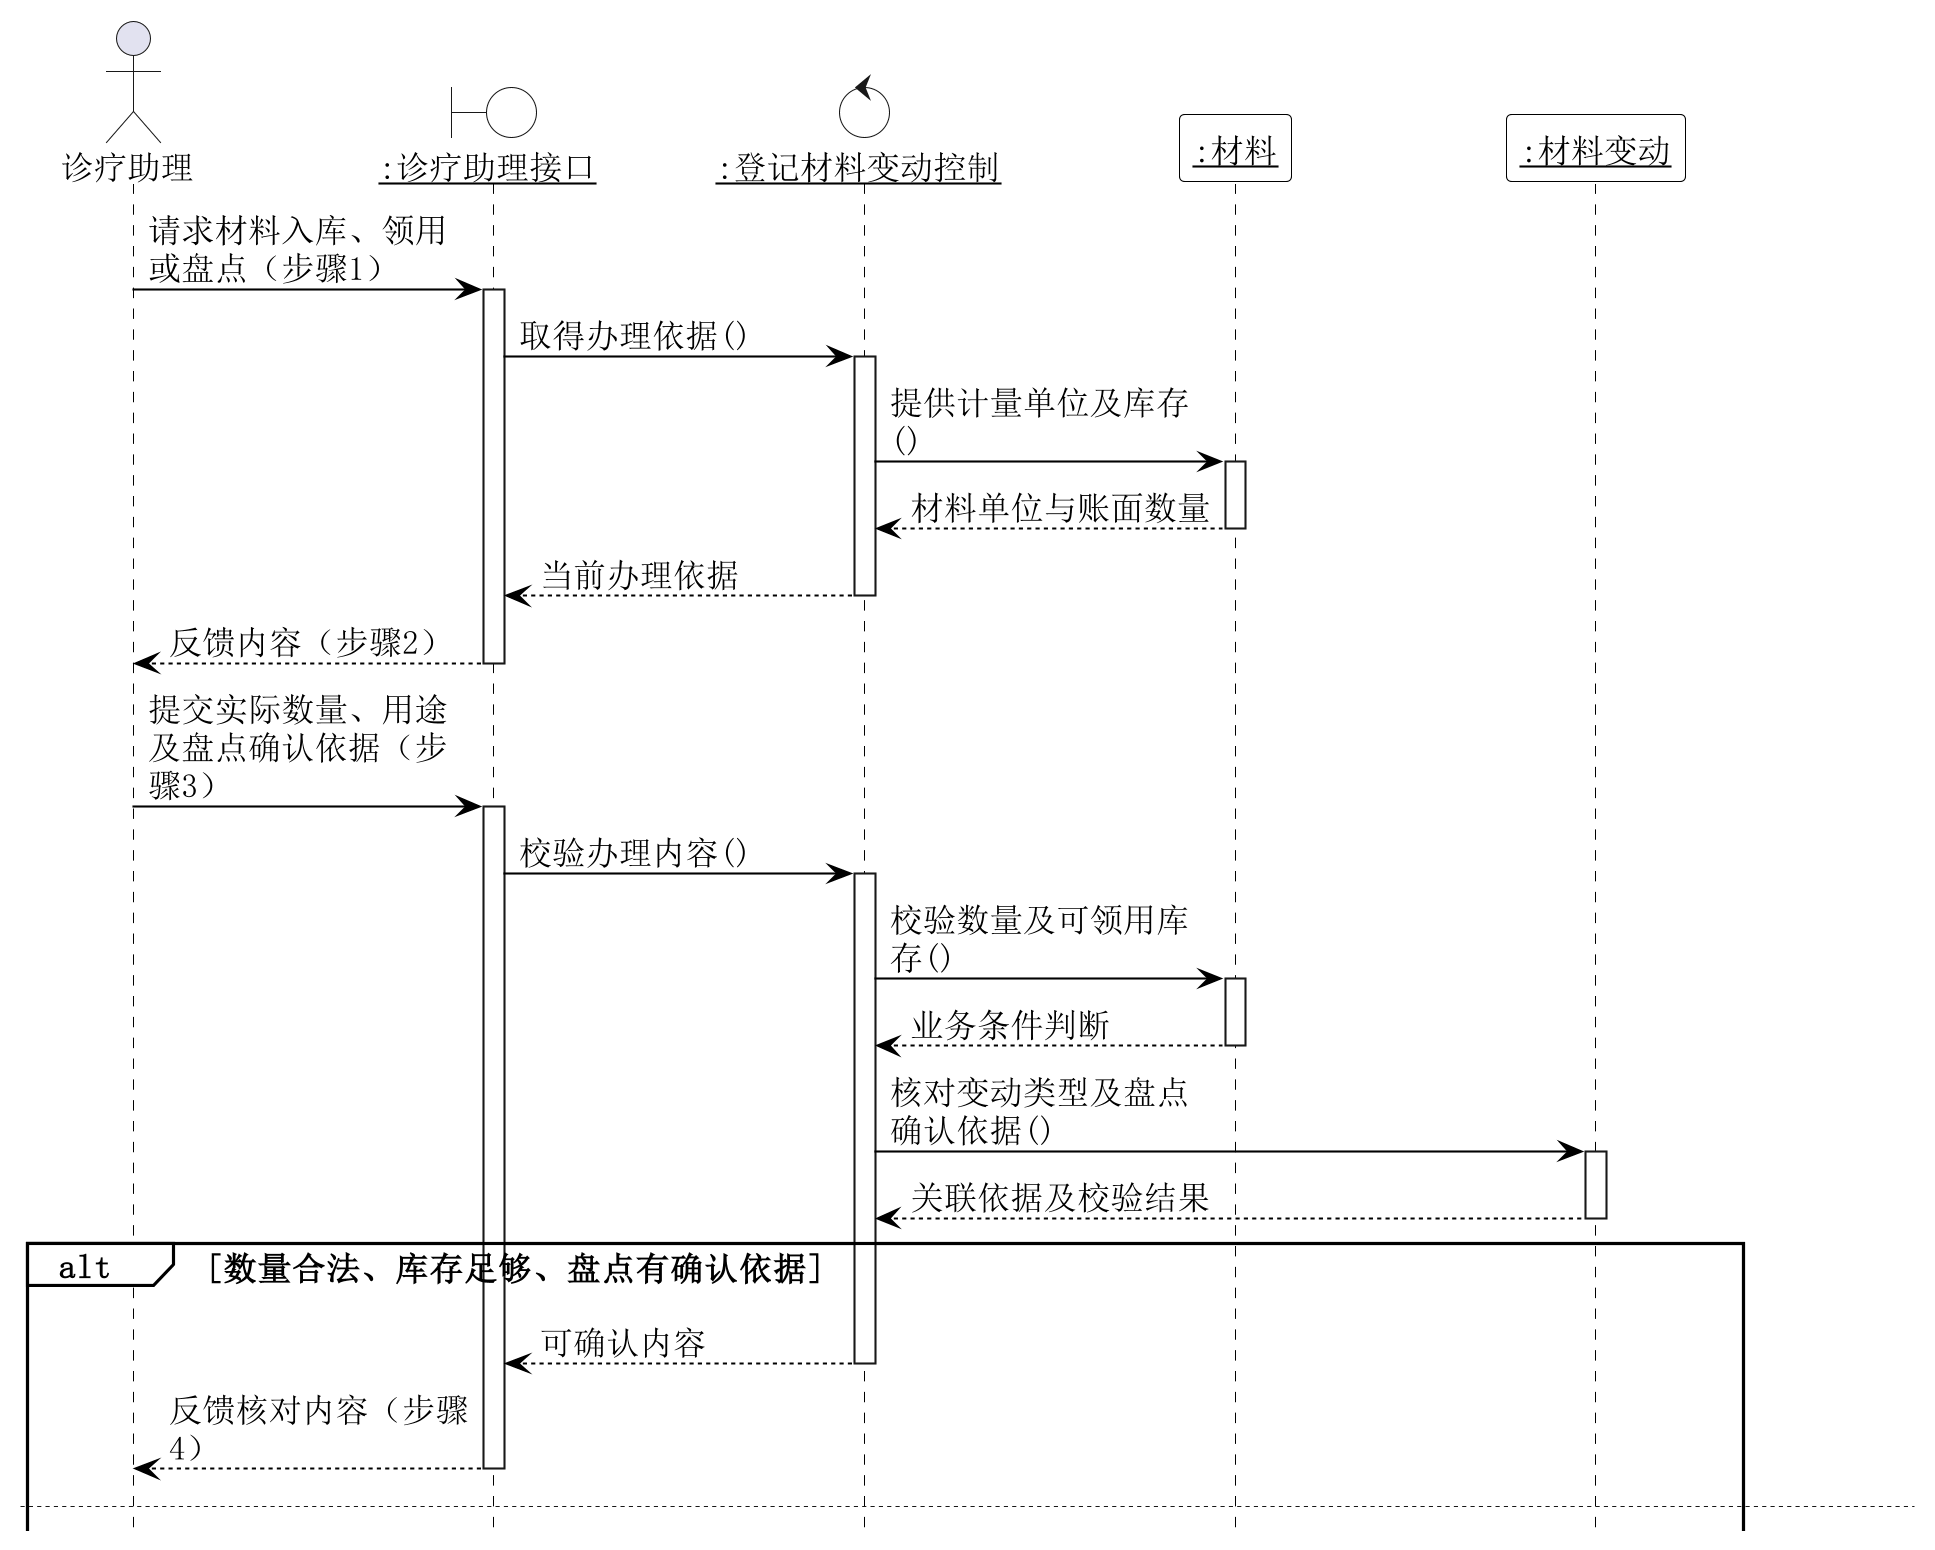
\includegraphics[width=\textwidth,height=20cm,keepaspectratio]{diagrams/13-18-analysis-sequence.png}
\caption{UC-18 登记材料变动分析序列图}
\label{fig:seq-18}
\end{figure}
\clearpage
\noindent\textbf{UC-18 分析序列图（续）}
\begin{figure}[!htbp]
\centering
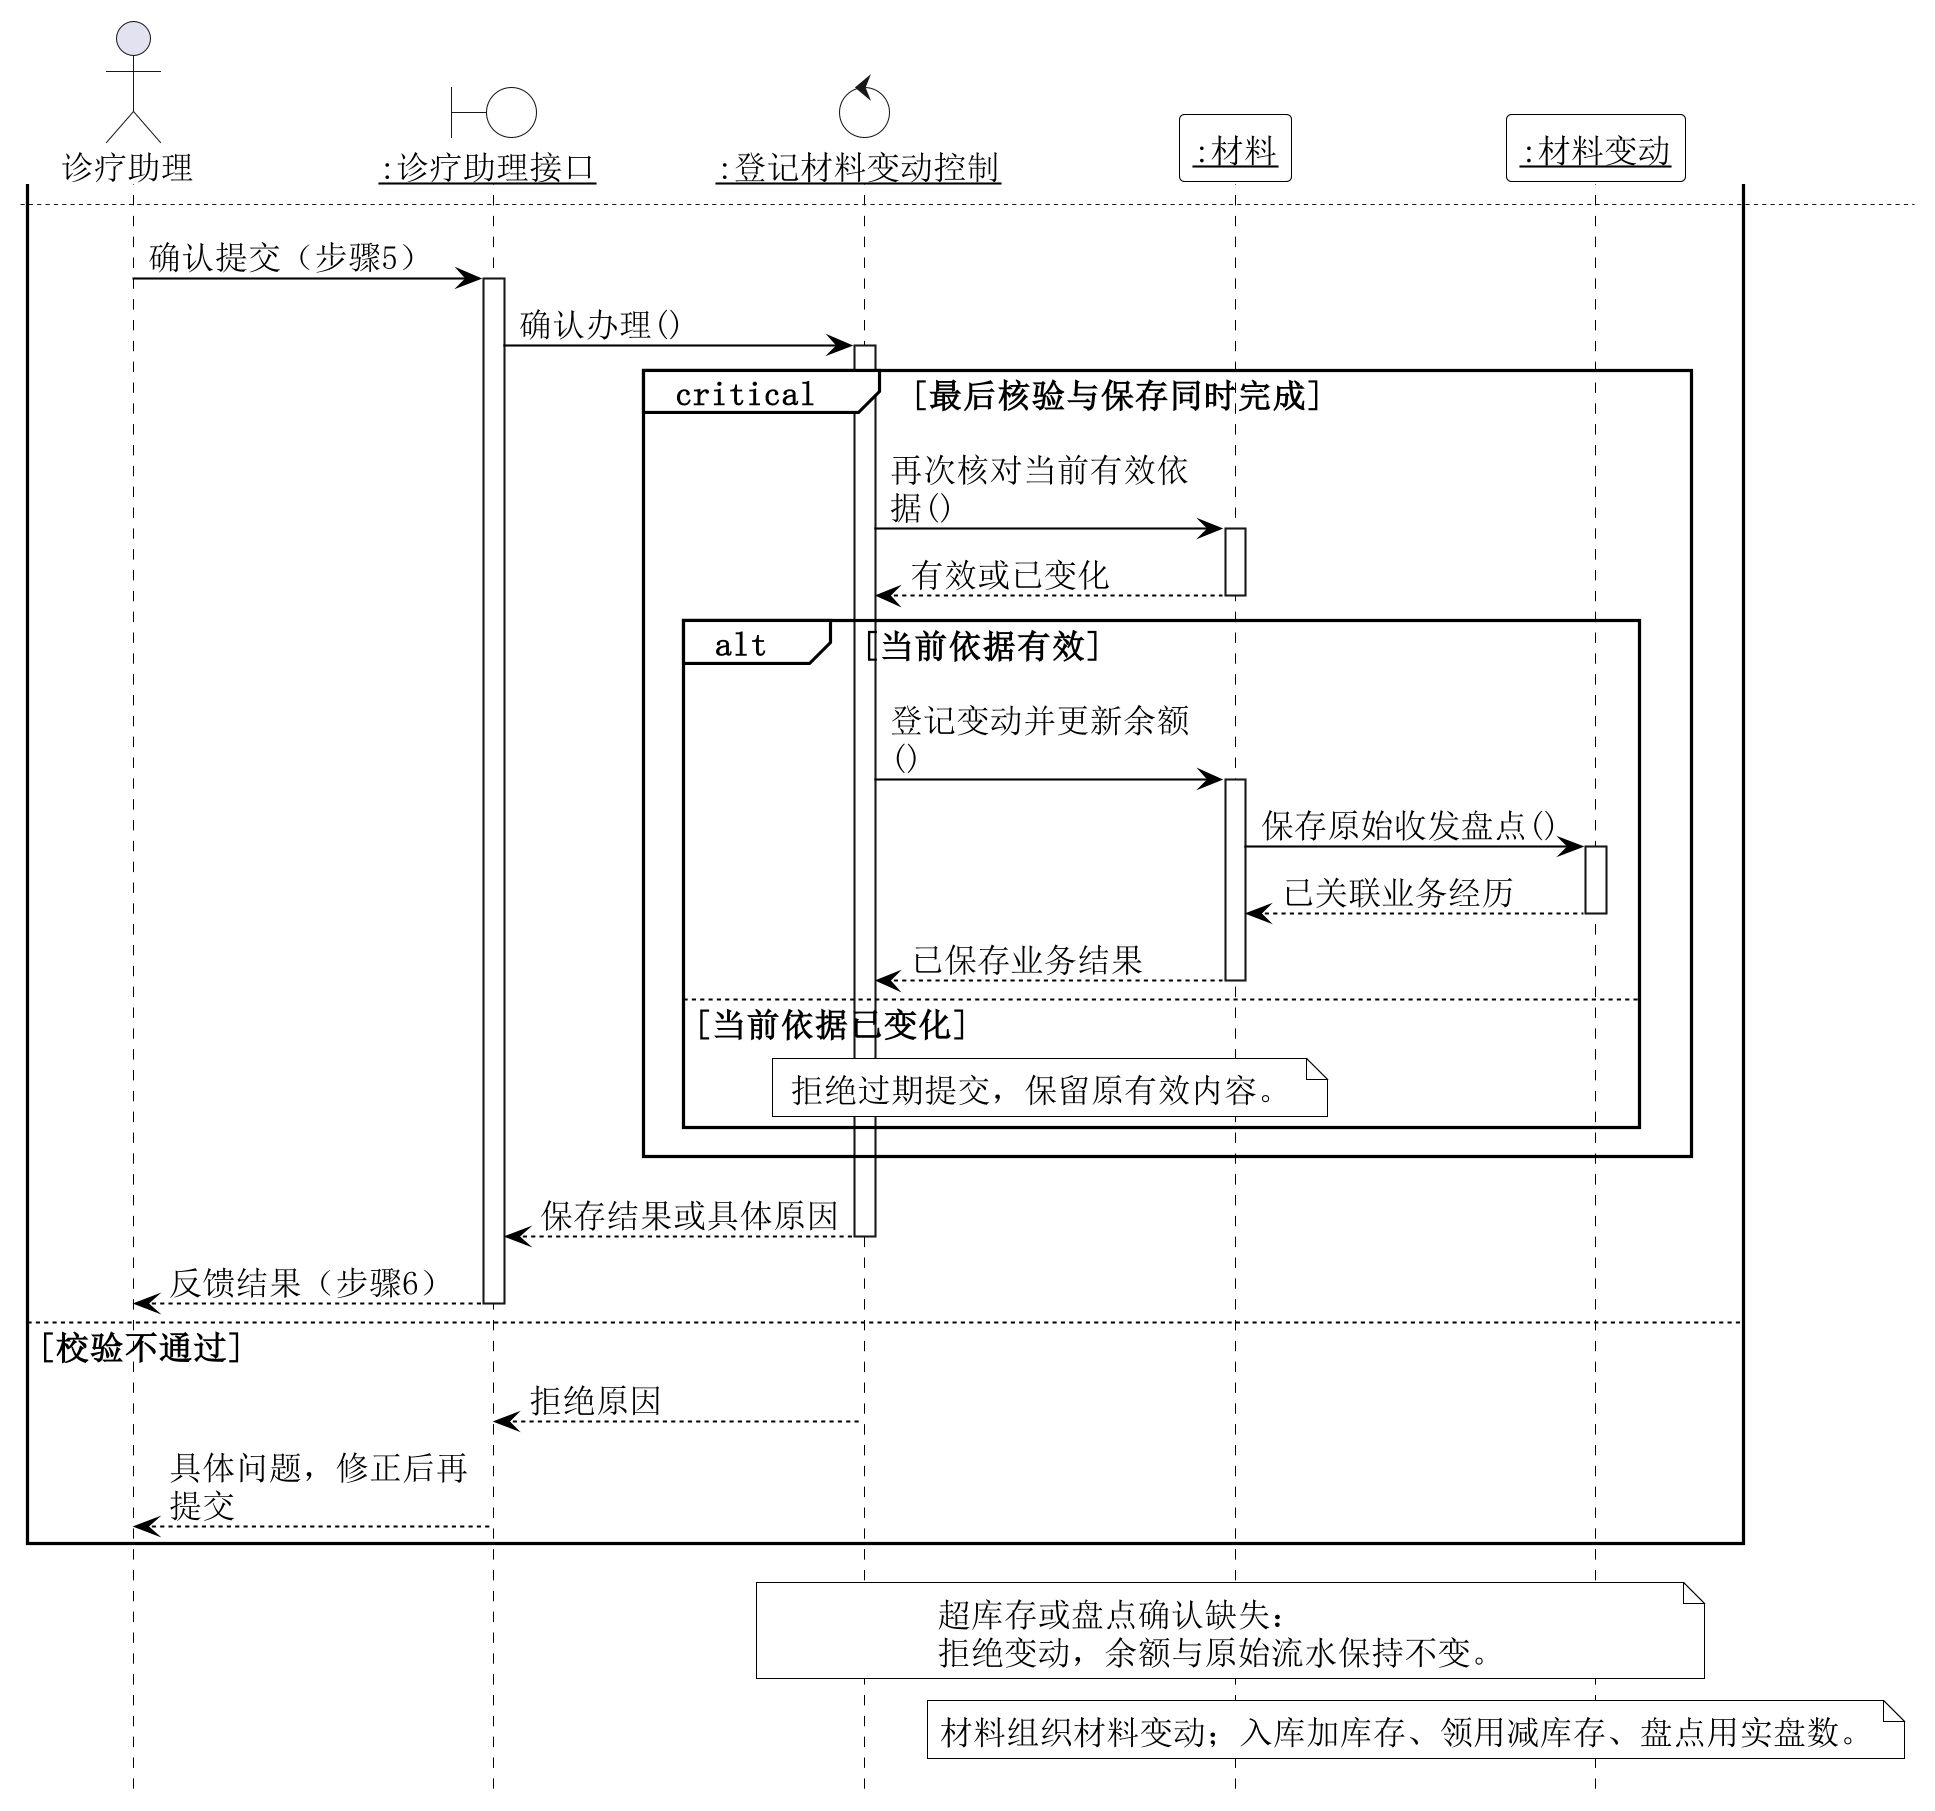
\includegraphics[width=\textwidth,height=20.4cm,keepaspectratio]{diagrams/13-18-analysis-sequence_001.png}
{\normalsize 图\ref{fig:seq-18}（续）：确认与保存}
\end{figure}
\clearpage
\subsubsection{UC-19：查询日常业务与收款}

本图按规约分配就诊、诊疗确认、诊疗明细、现金收款的业务责任。
\begin{figure}[!htbp]
\centering
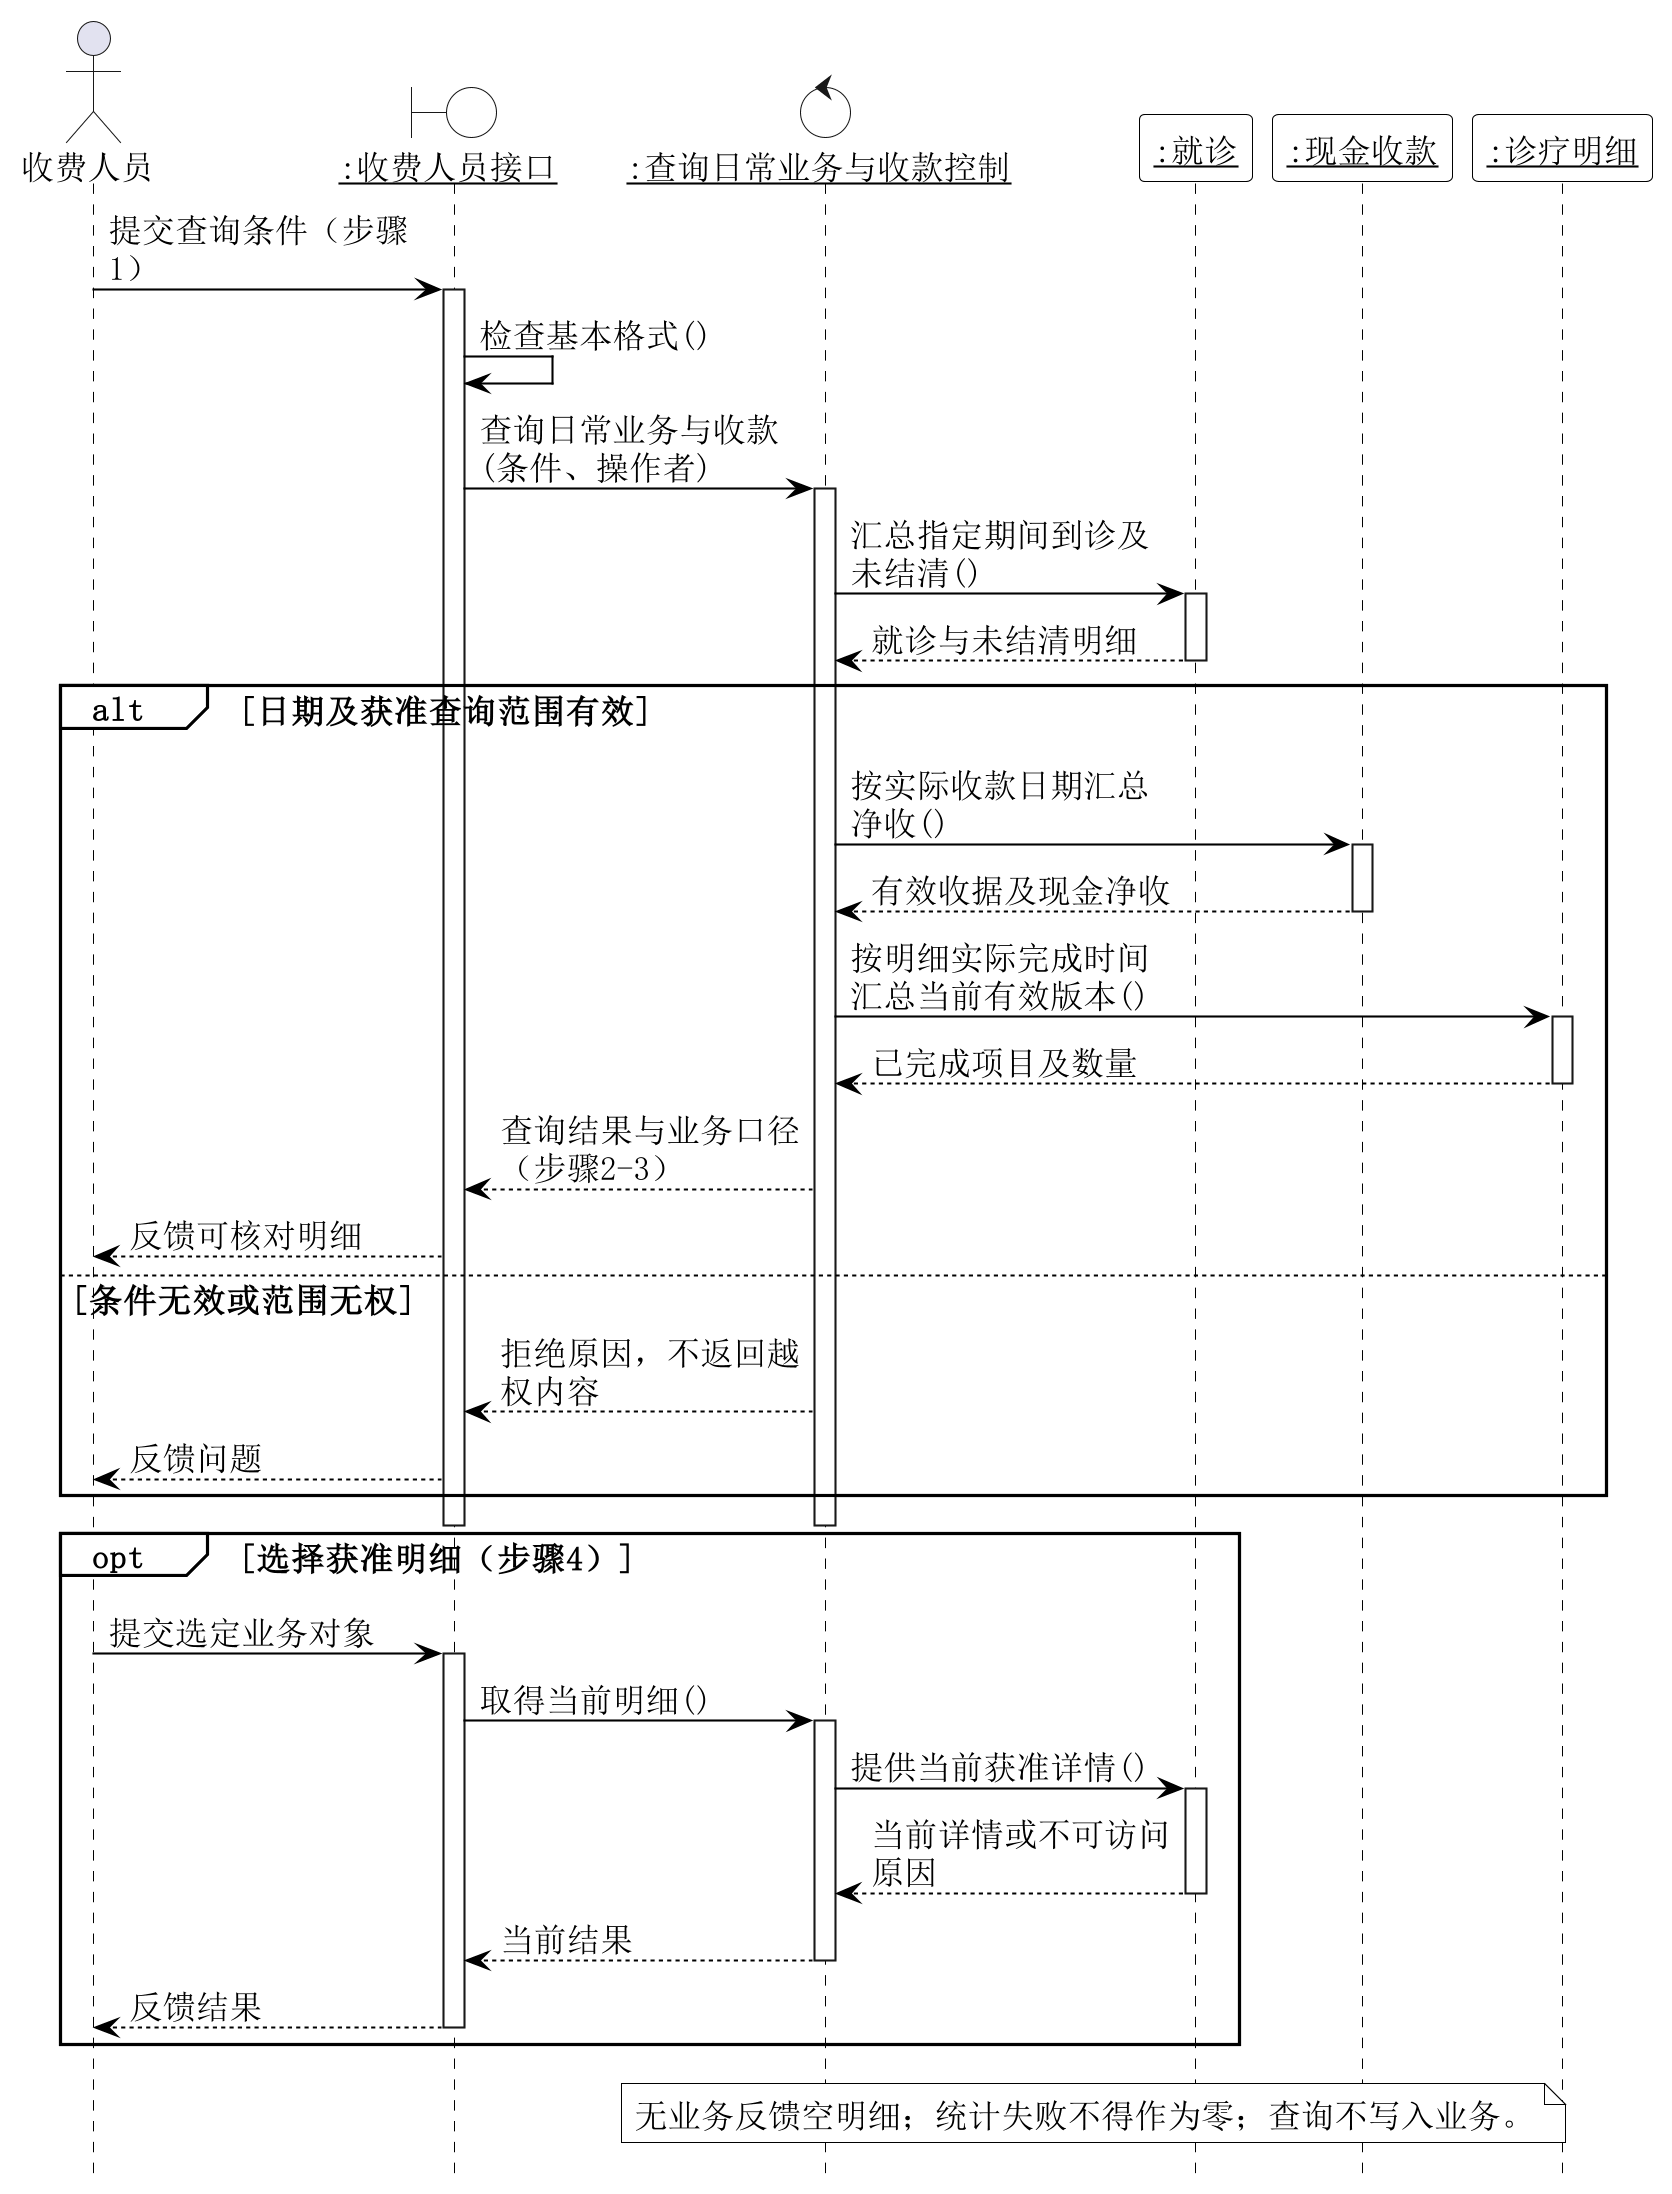
\includegraphics[width=\textwidth,height=20cm,keepaspectratio]{diagrams/13-19-analysis-sequence.png}
\caption{UC-19 查询日常业务与收款分析序列图}
\label{fig:seq-19}
\end{figure}
\clearpage
\begin{figure}[!htbp]
\centering
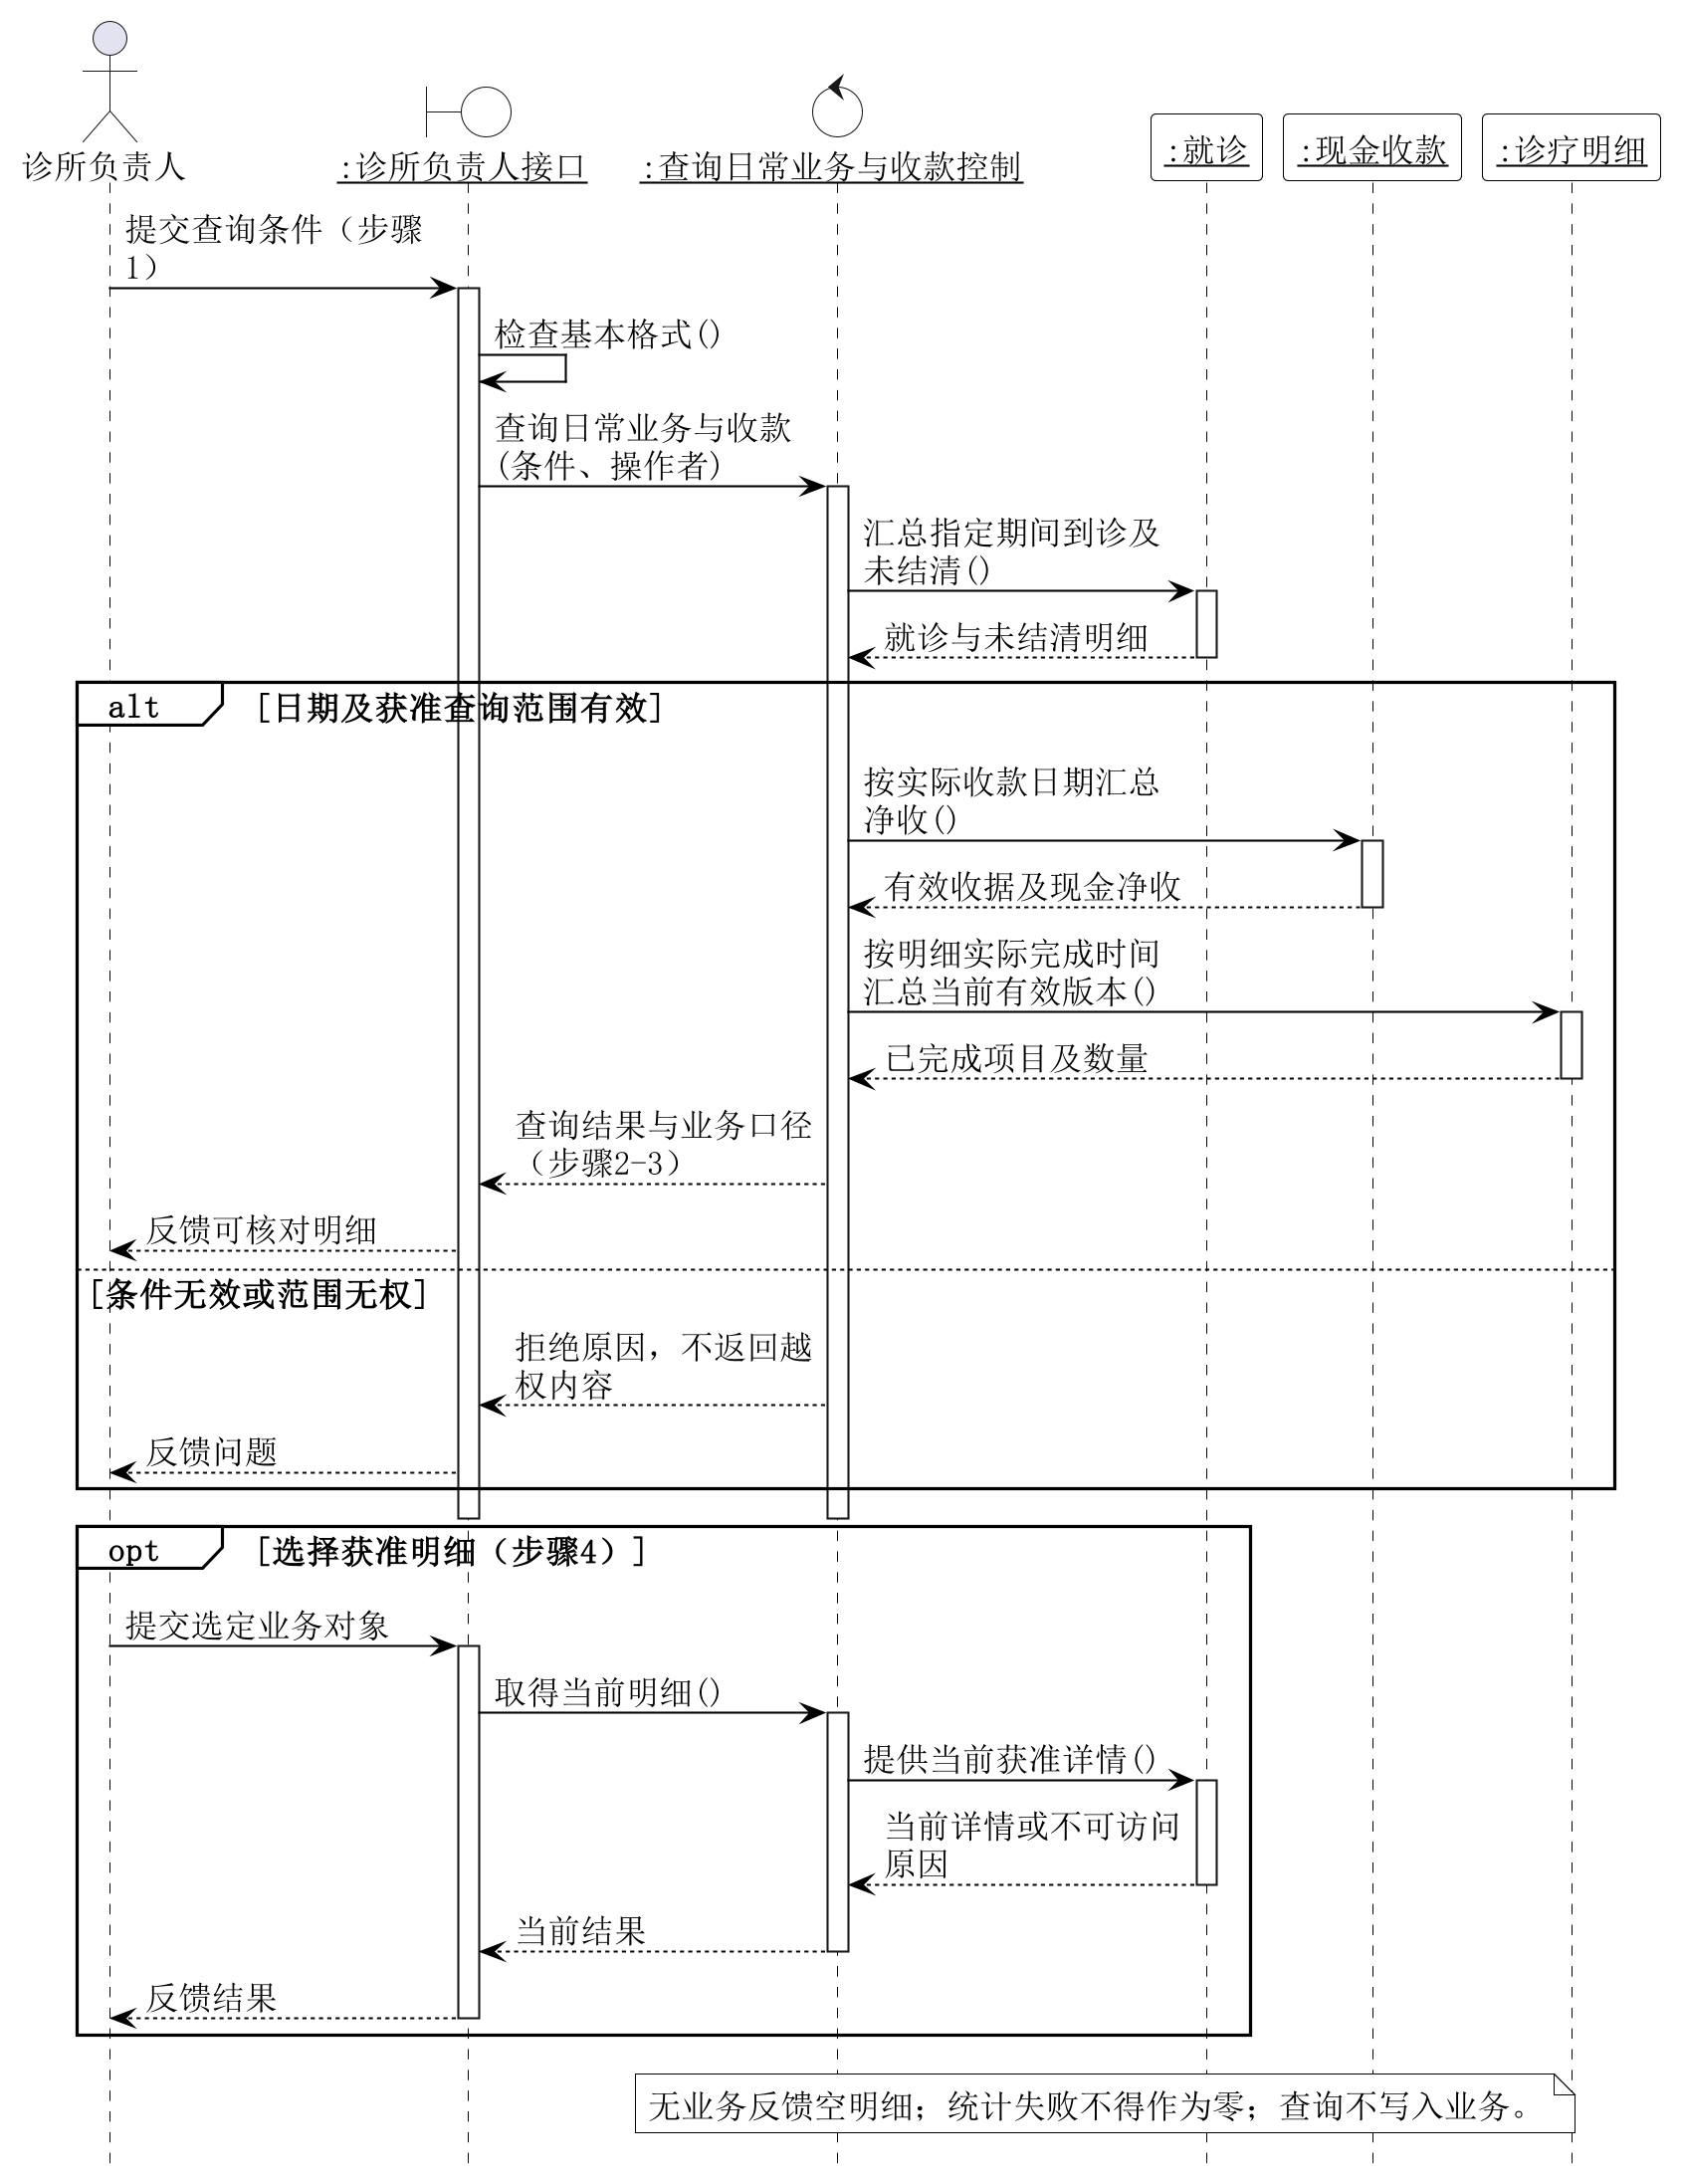
\includegraphics[width=\textwidth,height=20cm,keepaspectratio]{diagrams/13-19-alt-analysis-sequence.png}
\caption{UC-19 诊所负责人查询分析序列图}
\label{fig:seq-19-alt}
\end{figure}
\clearpage
\subsubsection{UC-20：登记收款核对}

本图按规约分配现金收款、收款核对、职员的业务责任。
\begin{figure}[!htbp]
\centering
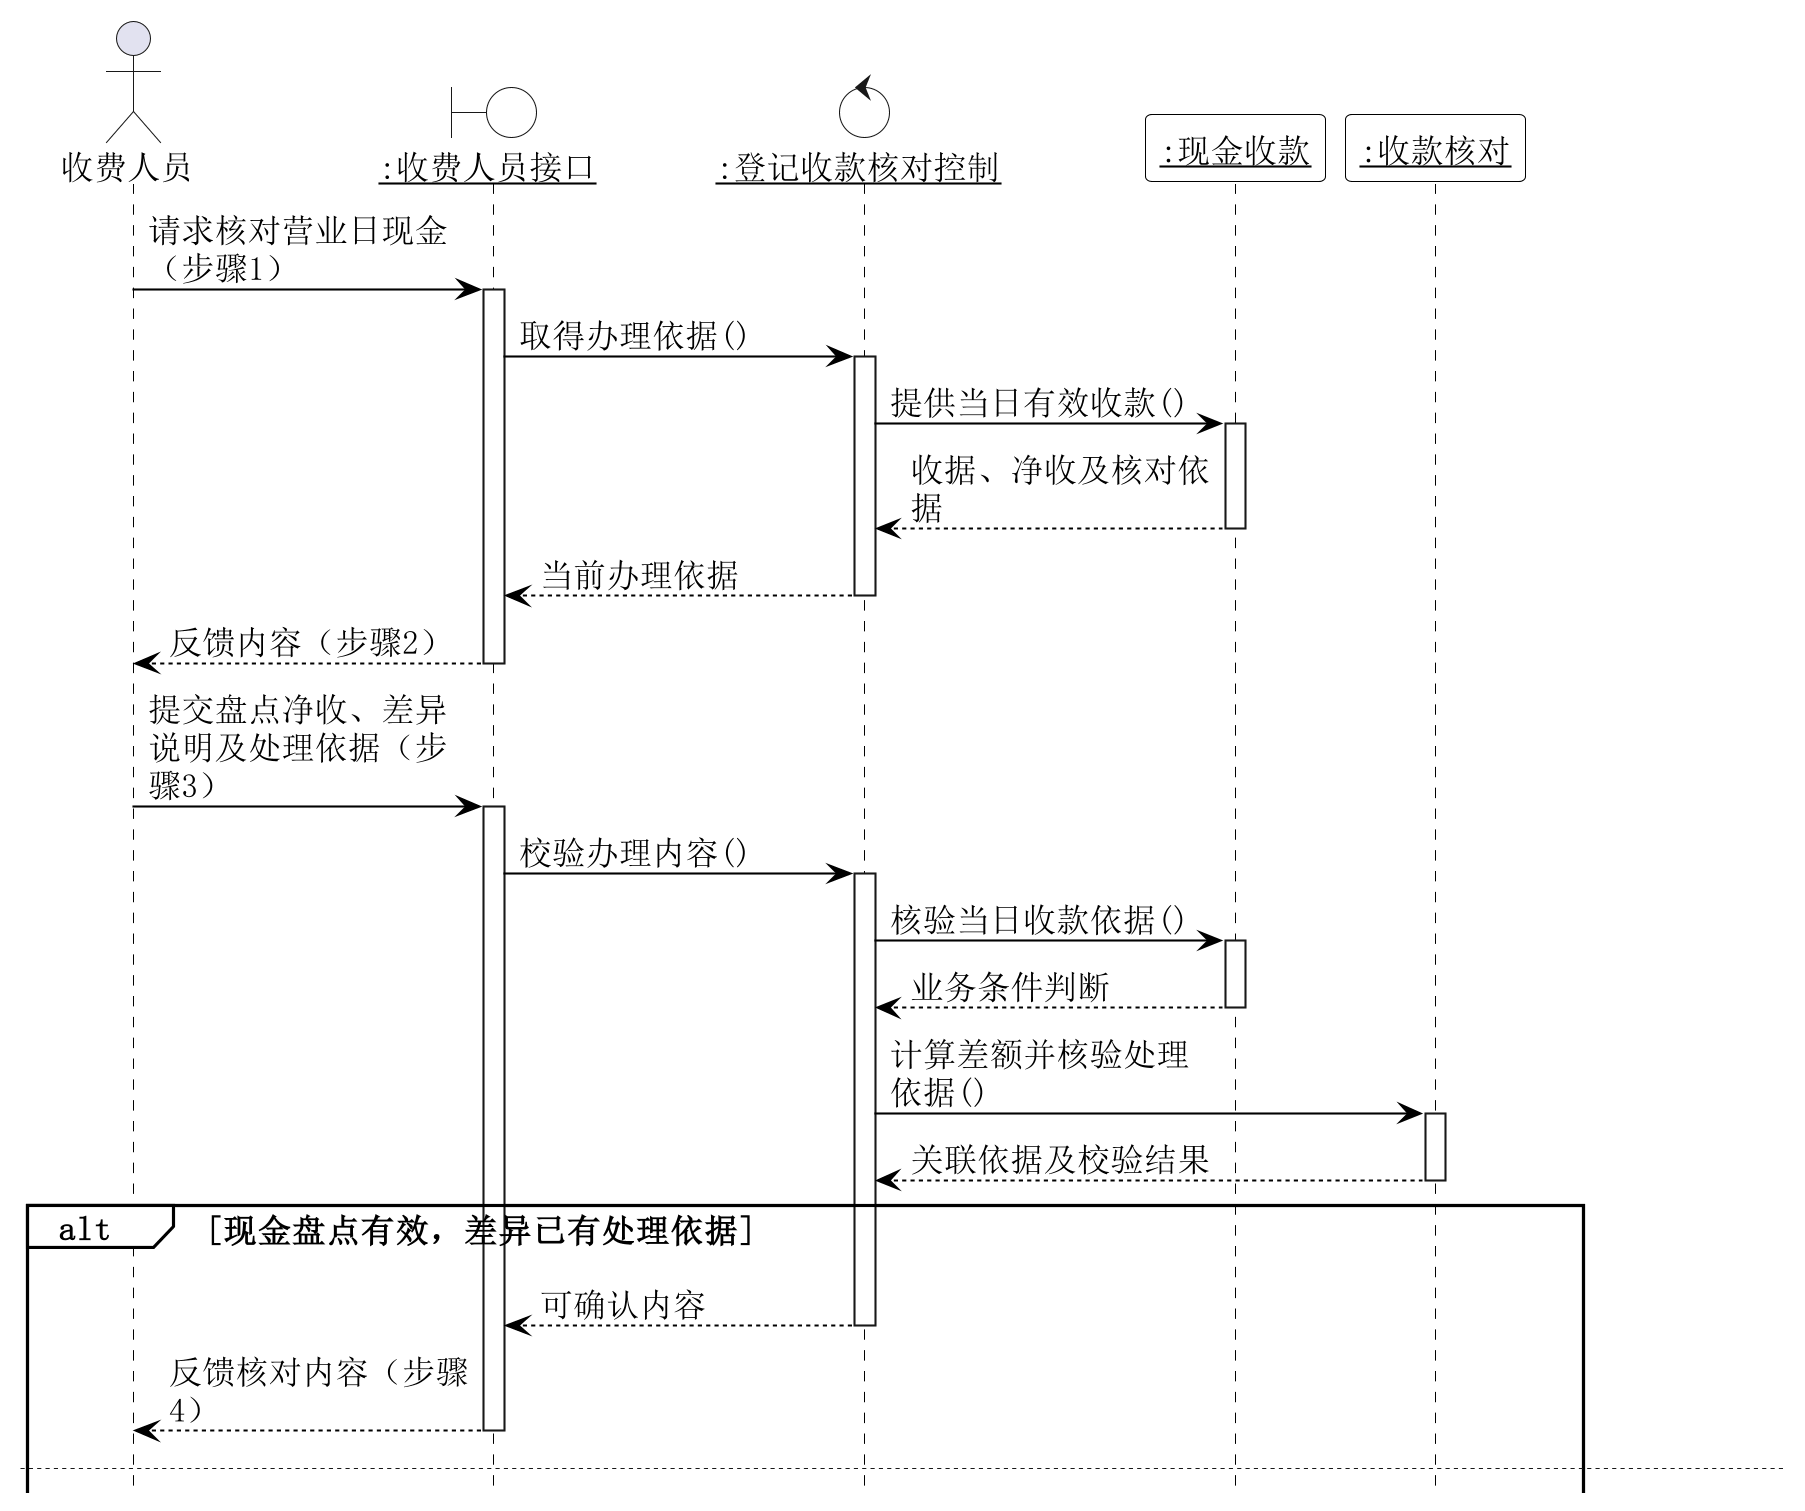
\includegraphics[width=\textwidth,height=20cm,keepaspectratio]{diagrams/13-20-analysis-sequence.png}
\caption{UC-20 登记收款核对分析序列图}
\label{fig:seq-20}
\end{figure}
\clearpage
\noindent\textbf{UC-20 分析序列图（续）}
\begin{figure}[!htbp]
\centering
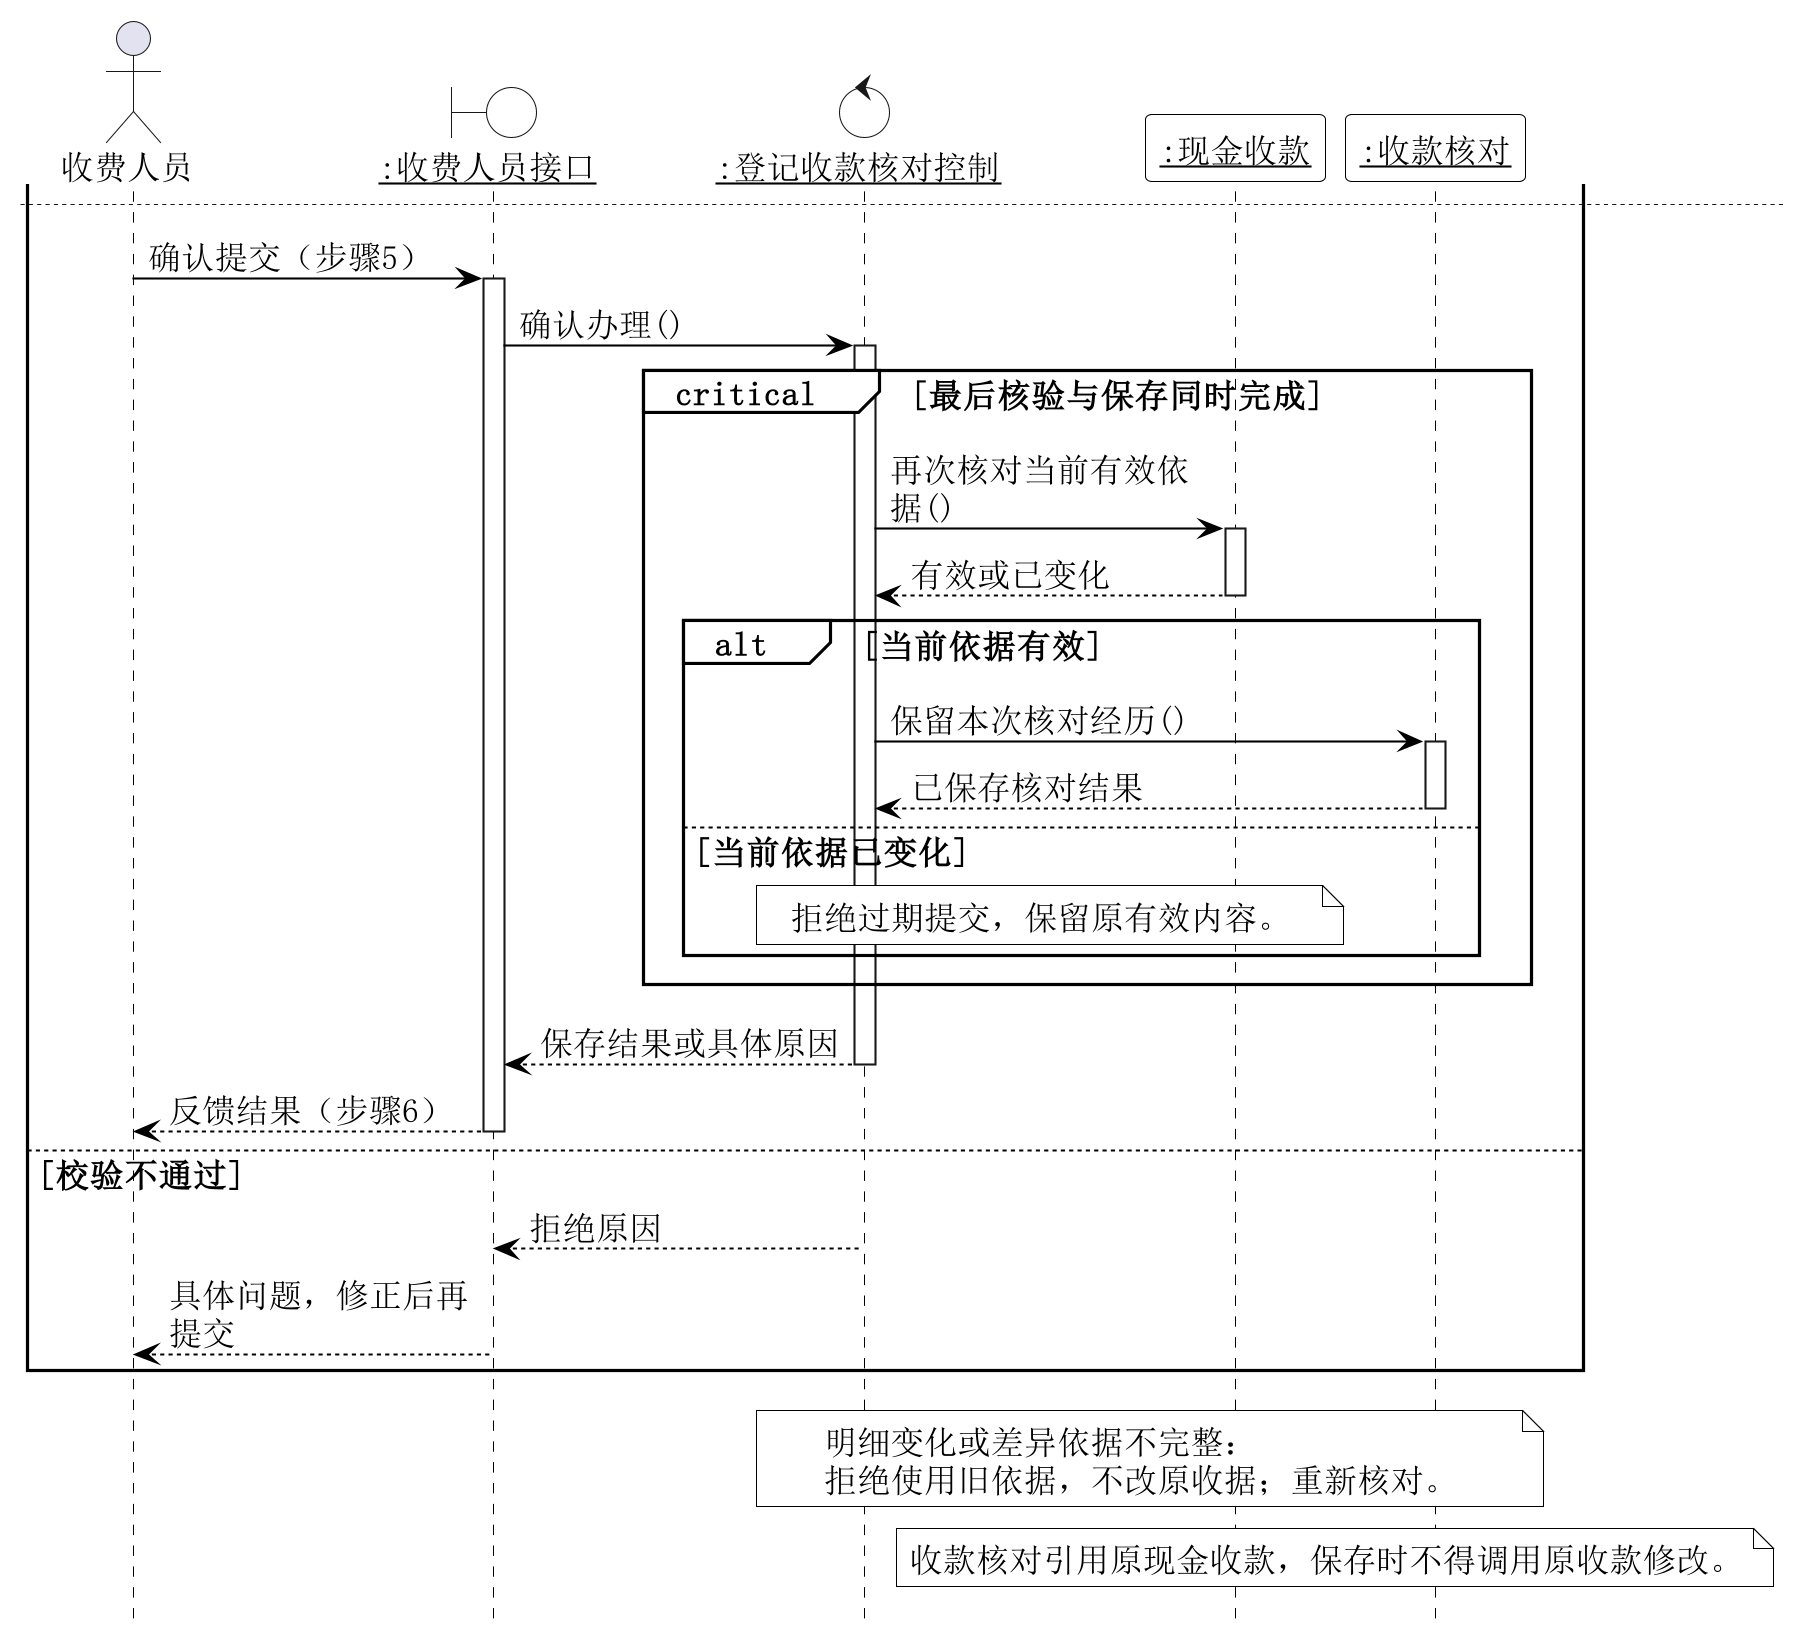
\includegraphics[width=\textwidth,height=20.4cm,keepaspectratio]{diagrams/13-20-analysis-sequence_001.png}
{\normalsize 图\ref{fig:seq-20}（续）：确认与保存}
\end{figure}
\clearpage
\subsubsection{用例路径与协作}

表\ref{tab:seq-index}列出各用例基本路径与扩展路径对应的分析序列图。

\begin{table}[htbp]
\centering
\caption{用例路径与分析序列图对应（UC-01至UC-07）}
\label{tab:seq-index}
\small
\renewcommand{\arraystretch}{1.3}
\begin{tabularx}{\textwidth}{@{}p{1.3cm}p{2.5cm}L@{}}
\toprule
用例 & 基本路径图 & 扩展路径处理 \\
\midrule
UC-01 & 图\ref{fig:seq-01} & 2a选定患者或建档后返回；4a合并基本图；1a、1b及6a见图\ref{fig:seq-01-ext}，取消关联预约同时返回待联系。 \\
UC-02 & 图\ref{fig:seq-02} & 2a、3a合并基本图；4a由前台核对选择，5a读取最新详情。 \\
UC-03 & 图\ref{fig:seq-03} & 3a停止确认；4a、4b合并基本图；5a按预约查询后恢复。 \\
UC-04 & 图\ref{fig:seq-04} & 2a、4a、6a合并基本图；4b及更正时的6a见图\ref{fig:seq-04-ext}；既有与新增明细计价见图\ref{fig:seq-04-pricing}。 \\
UC-05 & 图\ref{fig:seq-05} & 4a、6a合并基本图；3a、4b见图\ref{fig:seq-05-ext}。 \\
UC-06 & 图\ref{fig:seq-06} & 2a、4a、4b合并基本图；5a使旧核对依据失效，经本用例重新核对。 \\
UC-07 & 图\ref{fig:seq-07} & 2a、4a合并基本图；4b、5a、6a见图\ref{fig:seq-07-ext}。 \\
\bottomrule
\end{tabularx}
\end{table}

\clearpage
\begin{table}[!htbp]
\centering
\caption{用例路径与分析序列图对应（UC-08至UC-14）}
\label{tab:sequence-new-0}
\small
\renewcommand{\arraystretch}{1.18}
\begin{tabularx}{\textwidth}{@{}>{\raggedright\arraybackslash}p{1.3cm}>{\raggedright\arraybackslash}p{3.2cm}L@{}}
\toprule
用例 & 分析图 & 扩展处理 \\
\midrule
UC-08 & 图\ref{fig:seq-08} & 2a 存在同名或相同电话；4a 必填资料缺失；6a 资料已被修改。 \\
UC-09 & 图\ref{fig:seq-09} & 2a 不属于本人接诊范围；2b 患者没有既往病历；4a 所选病历不可取得。 \\
UC-10 & 图\ref{fig:seq-10} & 3a 患者尚未决定或仅完成检查；4a 内容无效或就诊不符；6a 病历已签署或内容已变化。 \\
UC-11 & 图\ref{fig:seq-11} & 1a 已签署病历需要补充；4a 主诉、检查诊断或诊后内容缺失；6a 重复签署或原内容变化。 \\
UC-12 & 图\ref{fig:seq-12} & 2a 来源未签署或不属于本人；4a 无目的、日期或有效前台；6a 重复的同一提交。 \\
UC-13 & 图\ref{fig:seq-13} & 2a 原复诊预约取消后待联系；3a 未联系成功；3b 重新关联有效预约；3c 取消诊后要求；4a 要求或预约无效；6a 内容已被办理。 \\
UC-14 & 图\ref{fig:seq-14} & 2a 要求已取消或已完成；4a 预约复诊尚无已签署病历；4b 无权限或评估内容缺失；6a 重复确认同一评估。 \\
\bottomrule
\end{tabularx}
\end{table}
\clearpage
\begin{table}[!htbp]
\centering
\caption{用例路径与分析序列图对应（UC-15至UC-20）}
\label{tab:sequence-new-1}
\small
\renewcommand{\arraystretch}{1.18}
\begin{tabularx}{\textwidth}{@{}>{\raggedright\arraybackslash}p{1.3cm}>{\raggedright\arraybackslash}p{3.2cm}L@{}}
\toprule
用例 & 分析图 & 扩展处理 \\
\midrule
UC-15 & 图\ref{fig:seq-15} & 4a 新安排不能覆盖有效预约；4b 人员无效或时段重复；6a 期间预约或安排已变化。 \\
UC-16 & 图\ref{fig:seq-16}、图\ref{fig:seq-16-alt} & 2a 日期或人员条件无效；3a 没有可接诊安排；4a 详情已变化。 \\
UC-17 & 图\ref{fig:seq-17}、图\ref{fig:seq-17-alt} & 2a 材料不存在或条件无效；3a 没有期间变动。 \\
UC-18 & 图\ref{fig:seq-18} & 3a 登记盘点调整；4a 领用超过可用库存；4b 材料无效、数量非法或确认缺失；6a 库存已变化。 \\
UC-19 & 图\ref{fig:seq-19}、图\ref{fig:seq-19-alt} & 2a 日期非法或范围无权；3a 没有相关业务；4a 需要核对差异。 \\
UC-20 & 图\ref{fig:seq-20} & 4a 盘点金额不合法或差异说明缺失；5a 尚未确定差异原因及处理意见；6a 该日收款明细已变化；6b 重复提交同一次核对。 \\
\bottomrule
\end{tabularx}
\end{table}

诊疗方案委托方案项目判断患者同意及剩余数量；病历维护原文及补充；诊后要求组织联系和评估；材料组织收发盘点经历；收款核对引用原收款。错误请求不得绕过这些实体判断。

预约保存、到诊登记、诊疗确认、价目调整和现金结算的同时生效约束均包括最后一次业务校验。失败保留原有效内容；并发操作不得绕过时段冲突、版本一致及唯一到诊或收款约束。分析图描述这些操作的业务契约，具体数据层实现留待设计阶段确定。

诊疗明细按数量乘以已关联单价计算金额，诊疗确认汇总明细；现金收款计算找零及净收。诊疗确认与价目依据共同构成费用核对依据，项目更正或缺价补齐后须重新核对。收款时使用当前完整依据，不能单凭旧总额登记。

\clearpage
\subsubsection{分析操作的细化}

分析类图保留各类的核心属性与操作；序列图进一步分配了查询、校验、版本更正及结果恢复责任。下表补充相应操作，与对应实体视图中的同名类保持一致。

\begin{table}[htbp]
\centering
\caption{实体类在分析序列图中的责任细化}
\label{tab:analysis-operations}
\small
\renewcommand{\arraystretch}{1.25}
\begin{tabularx}{\textwidth}{@{}p{2.0cm}L@{}}
\toprule
实体类 & 序列图细化的业务操作及协作 \\
\midrule
患者 & 核对预约患者、查询匹配患者、提供接待资料；参与预约与就诊的身份定位。 \\
职员 & 确认接诊资格、提供接诊信息；按关联角色确定操作者及业务确认人。 \\
预约 & 新增预约、查询预约、提供接待详情、判断可修改或取消、关联到诊；检查冲突，修改或取消时委托预约变更保留原安排。 \\
预约变更 & 保留变更，关联原安排、原因及经办职员；与对应预约共同保持追溯内容。 \\
就诊 & 登记到诊并建立本次病历草稿，重复登记返回原对象；核对接诊归属，组织确认、更正和结算，关联当前有效确认与收款。 \\
接诊时段 & 提供覆盖预约时间的有效安排及牙医确认依据；发布、变更前核对人员资格及有效预约支持。 \\
方案项目 & 判断本次方案归属、患者同意及牙位；校验拟生效完整集合，数量仅按当前有效确认计算，历史更正版本不累计。 \\
诊后要求 & 组织联系和临床评估；当前复诊预约取消后，未终结要求返回待联系，原预约及取消依据继续保留。 \\
诊疗确认 & 校验拟生效完整集合、合并依据一致的同项目同牙位明细、保留历史确认；组织方案校验及计价协作，更正替换当前版本，历史数量不重复计入。 \\
诊疗明细 & 校验项目、牙位、数量及实际完成时间；委托方案项目判断同意及拟生效数量；继承原计价依据或按保存的时点匹配价目，并依数量计算金额。 \\
收费项目 & 检查项目有效性、提供现有或适用价目、检查并维护价目方案、停止适用、调整价目区间；作为价目整体组织各版本。 \\
价目 & 提供适用区间、核对已关联价目、提供已关联单价、新增版本及结束适用；检查完整方案的重叠情况，不覆盖历史单价。 \\
现金收款 & 检查现金金额、登记收款、查询有效收款、形成收据；计算找零及净收，重取结果沿用原收款编号。 \\
\bottomrule
\end{tabularx}
\end{table}

序列图中的原确认与新确认、原价目与新价目分别为同一实体类的不同版本对象。查询匹配患者、预约或就诊的消息作用于该实体的业务对象集合，返回集合结果；后续消息作用于已选定的对象。对象的取得与保存方式在数据层设计中精化。

边界类承担发起操作、检查格式、提示问题及展示结果；控制类的接收操作与相应用例保持一致，并协调图中各次业务请求。序列图不新增业务执行者或系统用例。预约取消、到诊与结清等生命周期见第\ref{sec:analysis-state}节。

\clearpage
\subsection{分析状态机图}
\label{sec:analysis-state}

\subsubsection{预约的状态机图}

图\ref{fig:appointment-state}描述单个预约对象。预约保存后处于已预约；调整安排保持该状态，取消和到诊分别进入已取消、已到诊。取消与到诊互斥，已取消或已到诊的预约均不得再调整为待到诊安排。

\begin{figure}[!htbp]
\centering
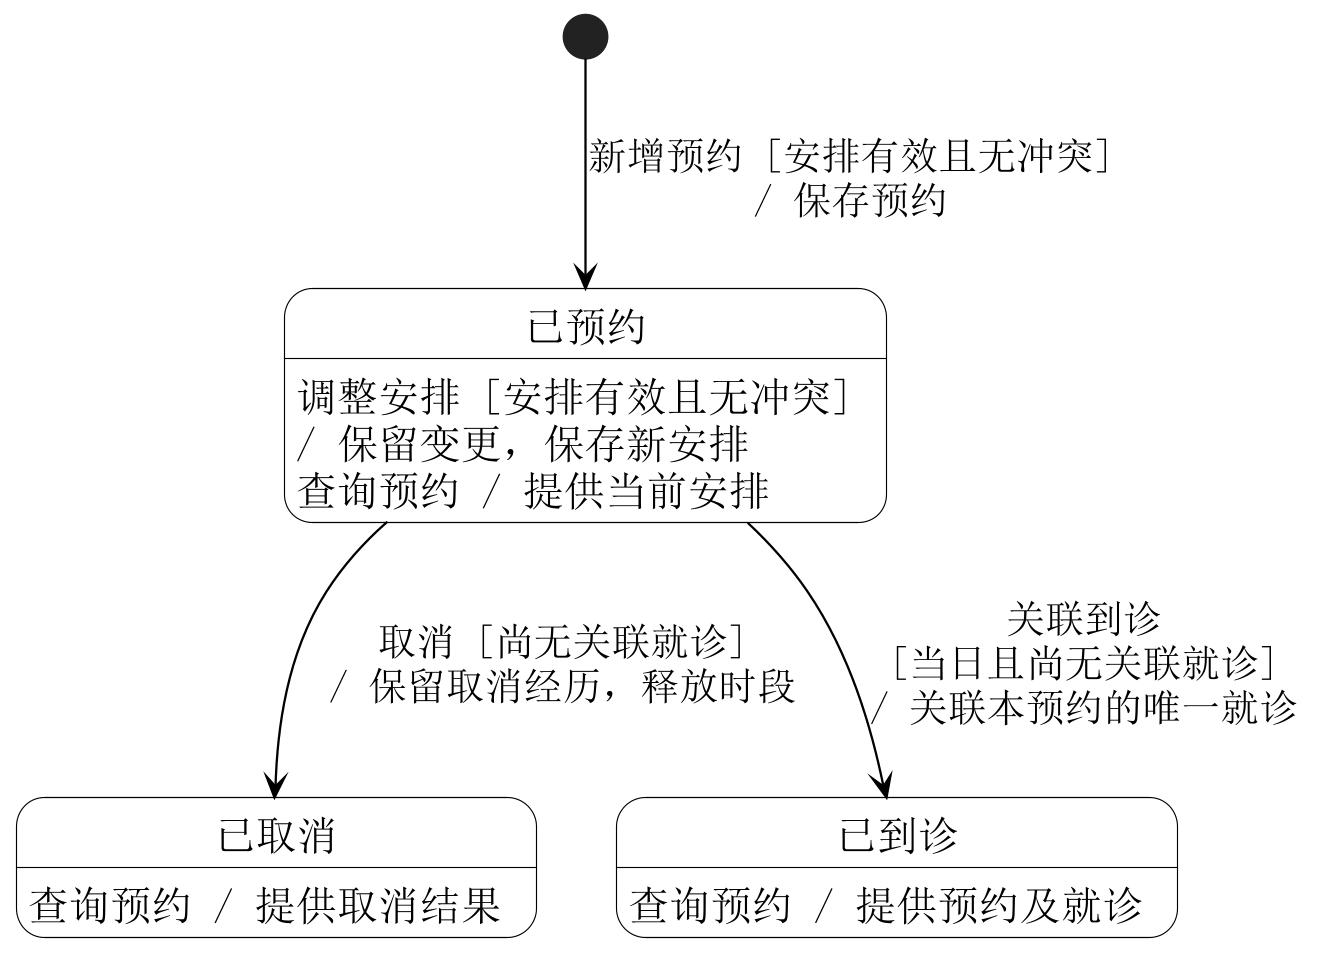
\includegraphics[width=\textwidth,height=9cm,keepaspectratio]{diagrams/14-appointment-state-machine.png}
\caption{预约的分析状态机图}
\label{fig:appointment-state}
\end{figure}

{\small
\renewcommand{\arraystretch}{1.2}
\noindent\begin{tabularx}{\textwidth}{@{}p{2cm}L@{}}
\toprule
状态 & 业务判定及限制 \\
\midrule
已预约 & 无取消经历且未关联就诊；允许查询、合规调整、取消或登记当日到诊。逾期未到诊不自动转为已取消。 \\
已取消 & 已保留取消经历且未关联就诊；原安排及变更经历可查询，原预约不再占用时段，不允许到诊或重新激活。 \\
已到诊 & 已关联唯一就诊；允许查询，重复到诊返回原结果，不允许修改或取消预约。 \\
\bottomrule
\end{tabularx}\par
}

图中安排有效指患者、牙医及时间资料符合UC-01的规则，且安排已由牙医确认。保存与调整在生效前复核最新内容和时段冲突。关联到诊与就诊登记同时生效，失败保持原状态。已取消与已到诊的预约继续保留供查询。

\clearpage
\subsubsection{就诊的状态机图}

图\ref{fig:visit-state}描述单个就诊对象。未结清的就诊按当前诊疗确认及明细价目关联分为未确认项目、已确认缺价和可结算；项目更正产生新的当前确认，再判断其价目是否完整。全部明细已有价目才能结算，单价为零的有效价目仍属于已具备计价依据。

\begin{figure}[!htbp]
\centering
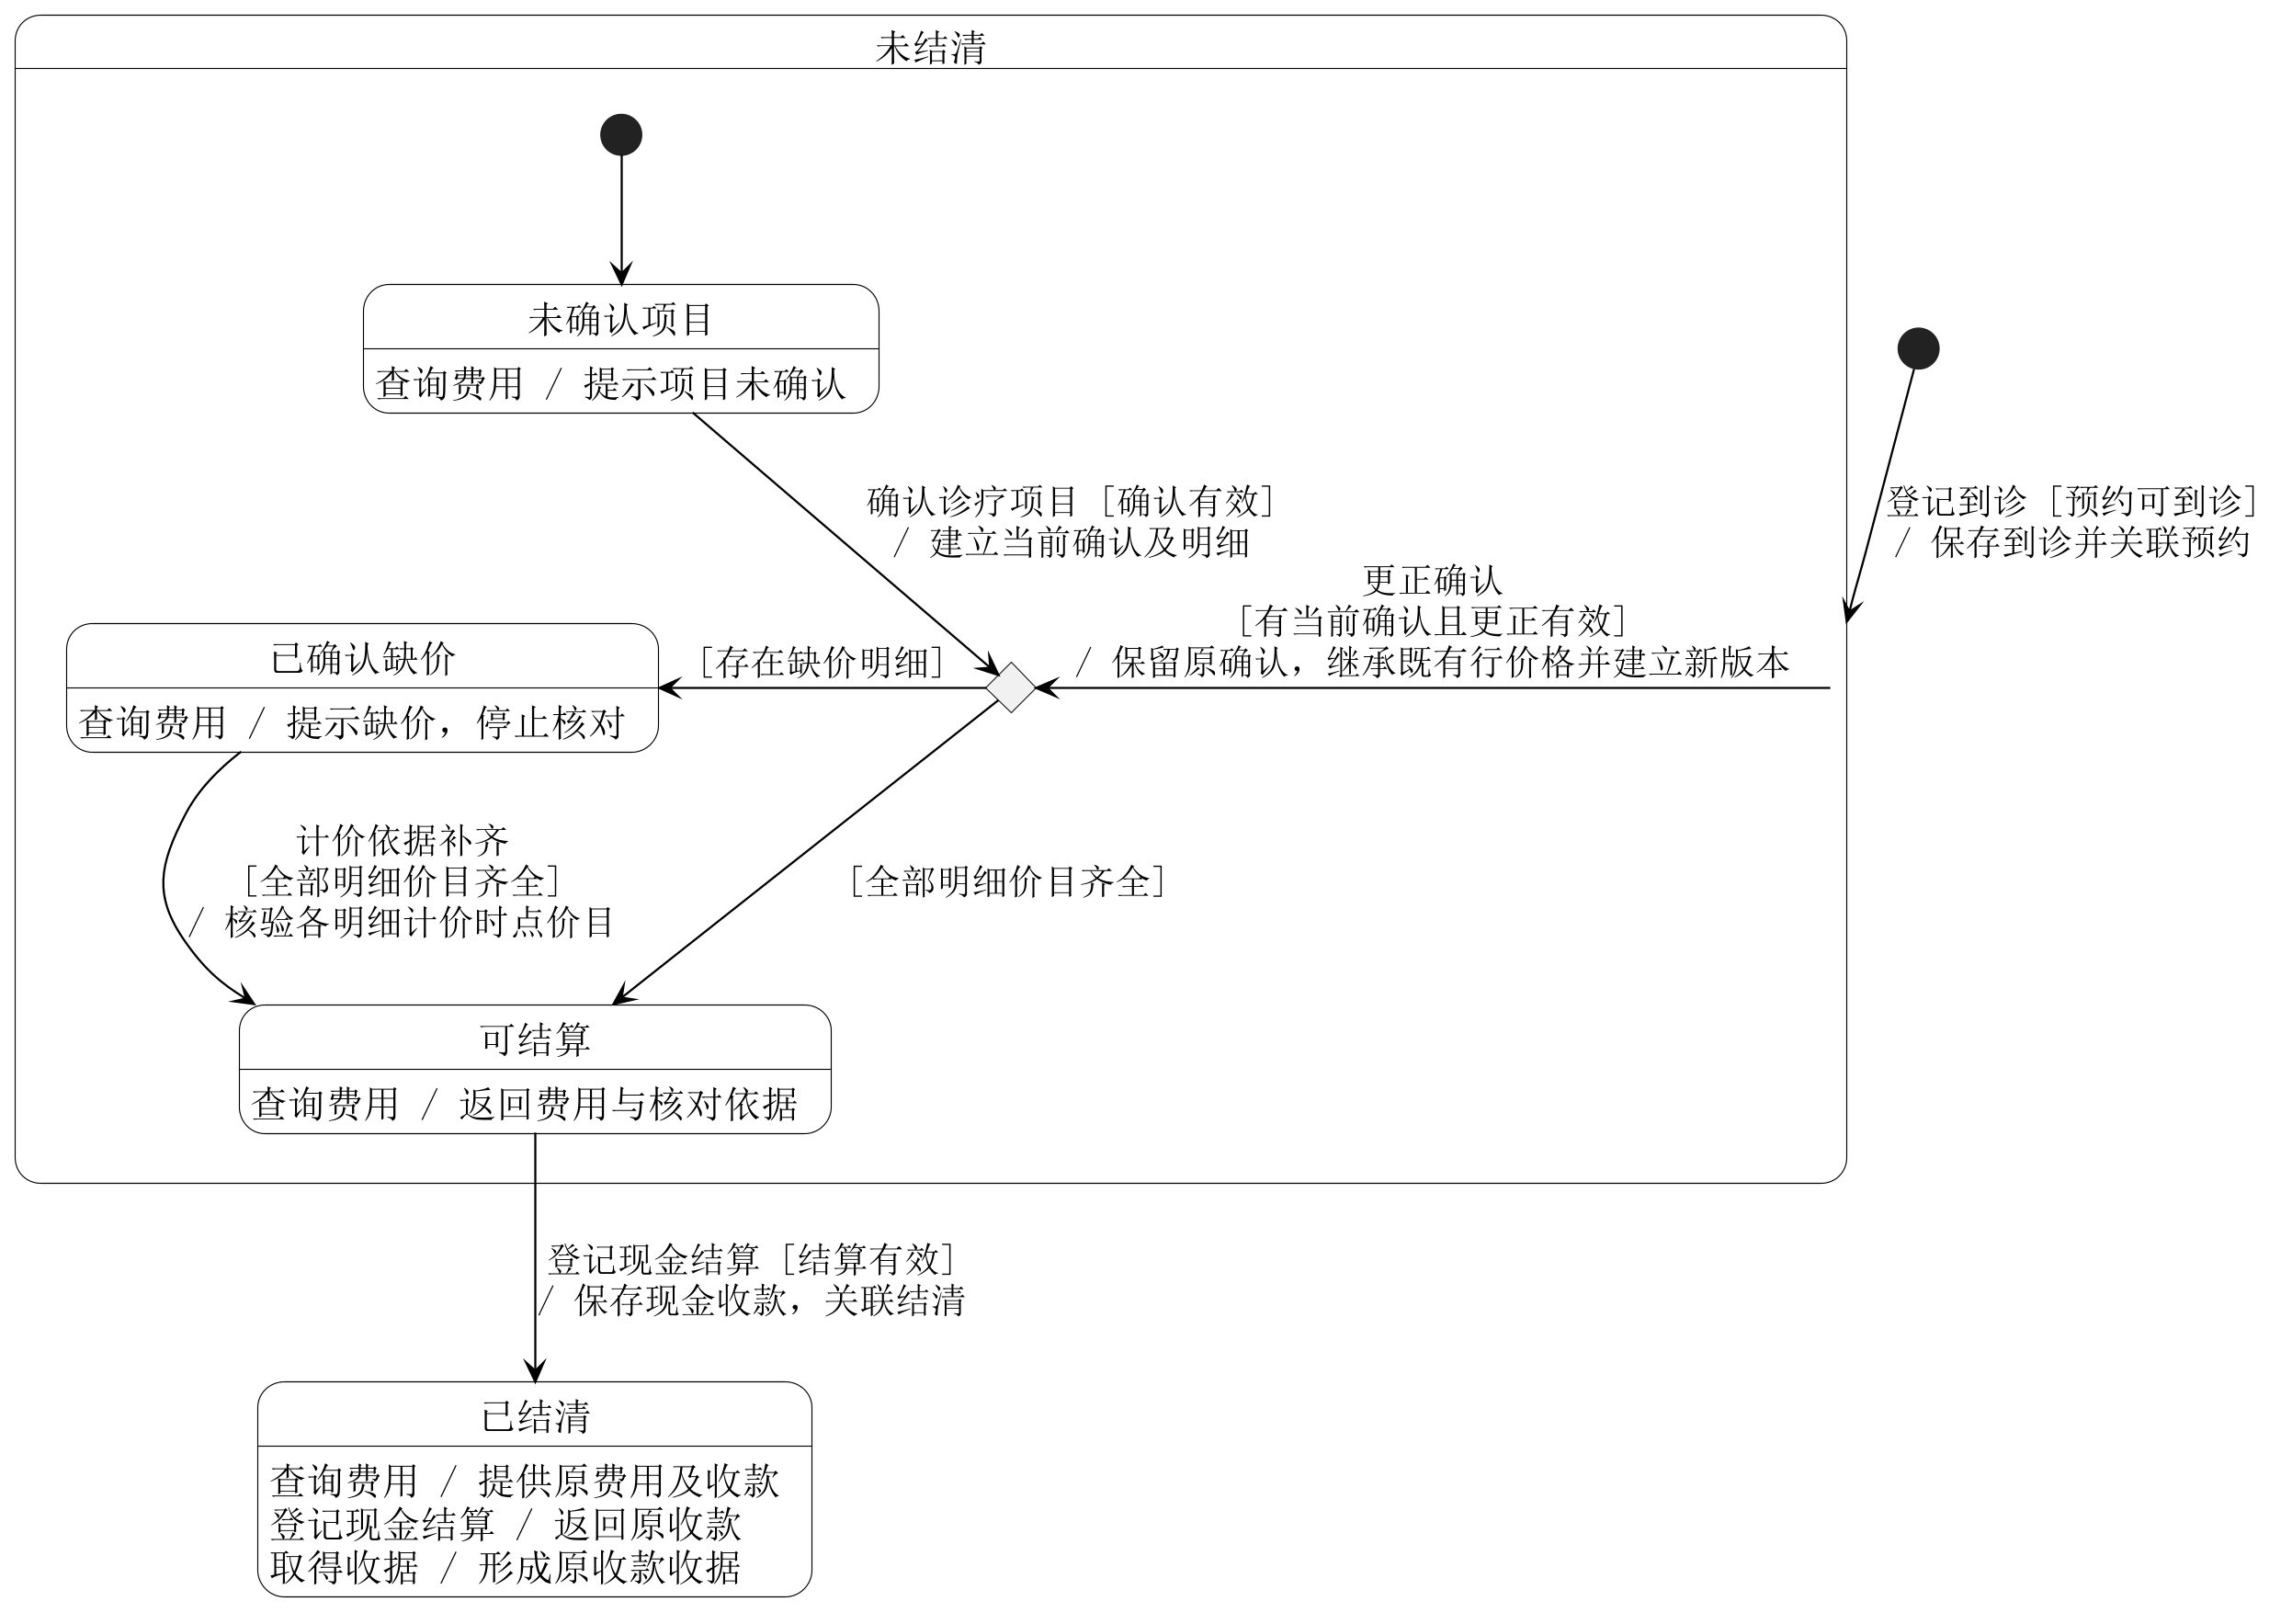
\includegraphics[width=\textwidth,height=17.8cm,keepaspectratio]{diagrams/15-visit-state-machine.png}
\caption{就诊的分析状态机图}
\label{fig:visit-state}
\end{figure}

图中确认有效、更正有效及结算有效的具体条件见表\ref{tab:state-guards}，“价目齐全”即全部明细已有适用价目。查询费用只返回结果；项目更正和缺价补齐后，原费用核对依据失效，收款前必须重新核对。已结清对象保留供查询及重新取得收据，不再进入未结清。

\clearpage
\clearpage
\subsubsection{病历的状态机图}

病历在登记到诊时建立草稿，UC-10保存临床内容，UC-11确认签署并锁定原文。补充为追加内容，不把病历退回草稿；病历生命周期与就诊的结算生命周期分别表达。
\begin{figure}[!htbp]
\centering
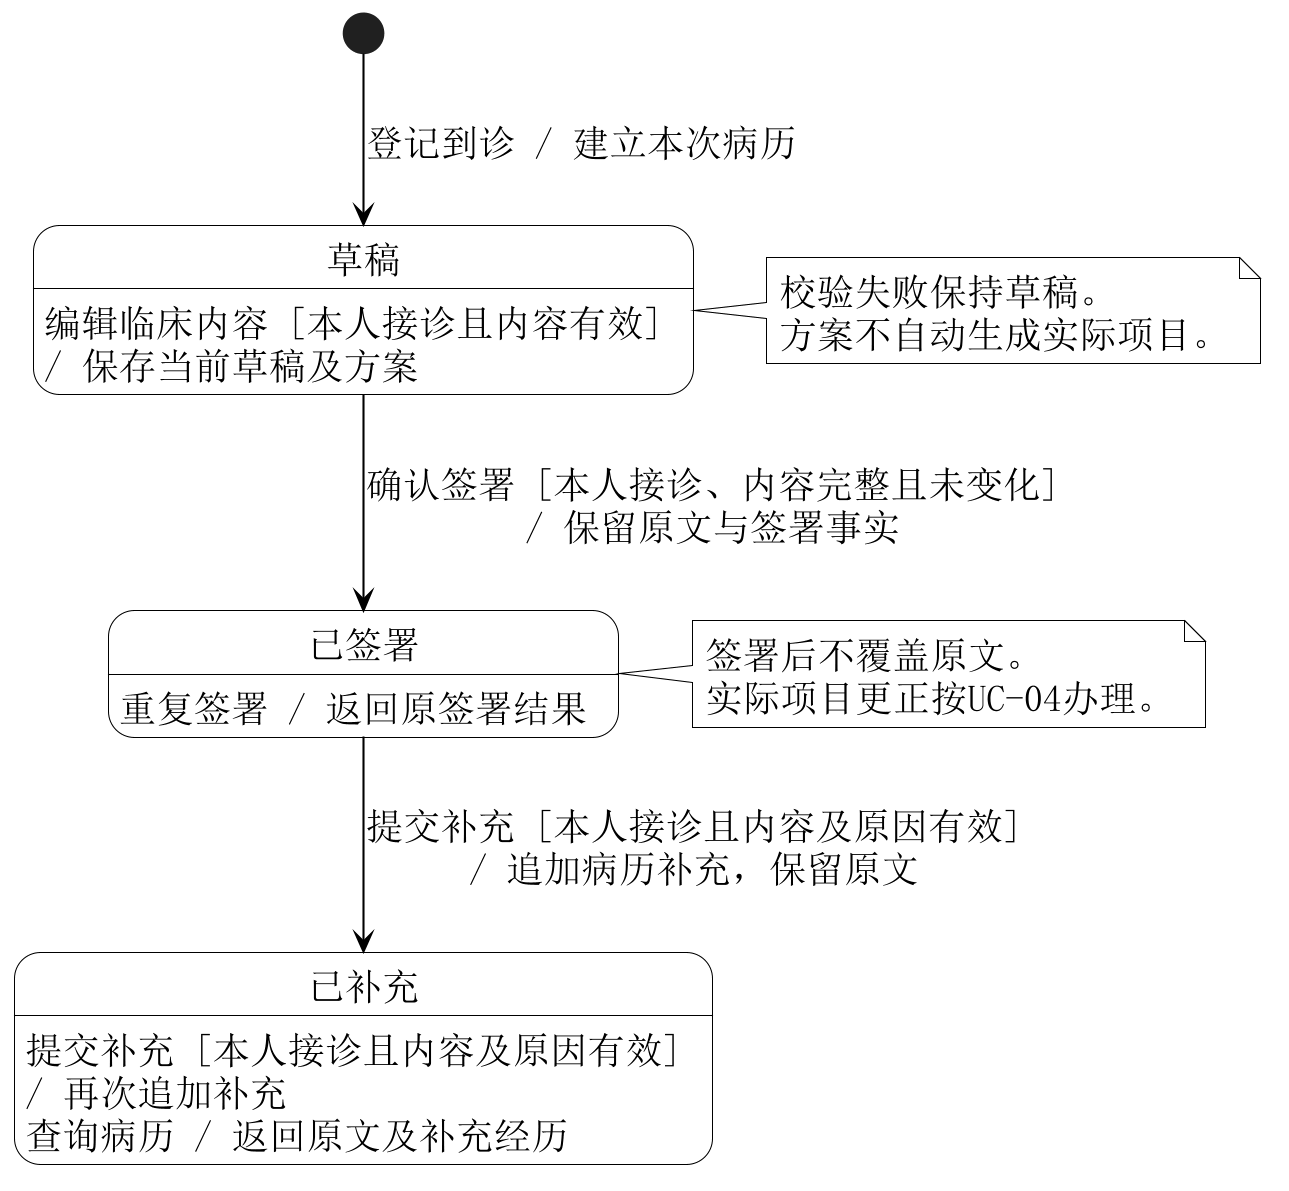
\includegraphics[width=\textwidth,height=18cm,keepaspectratio]{diagrams/16-clinical-state-machine.png}
\caption{病历的状态机图}
\label{fig:16-clinical-state-machine}
\end{figure}
\clearpage
\subsubsection{诊后要求的状态机图}

UC-12提出有来源的要求；UC-13保存联系及复诊关联；UC-14由有权限的牙医确认临床评估。前台不能将联系成功直接视为评估完成。要求取消与预约取消分别办理。当前复诊预约取消时，未终结要求返回待联系，保留原预约及取消依据；只有重新关联有效预约才再次进入已约复诊。
\begin{figure}[!htbp]
\centering
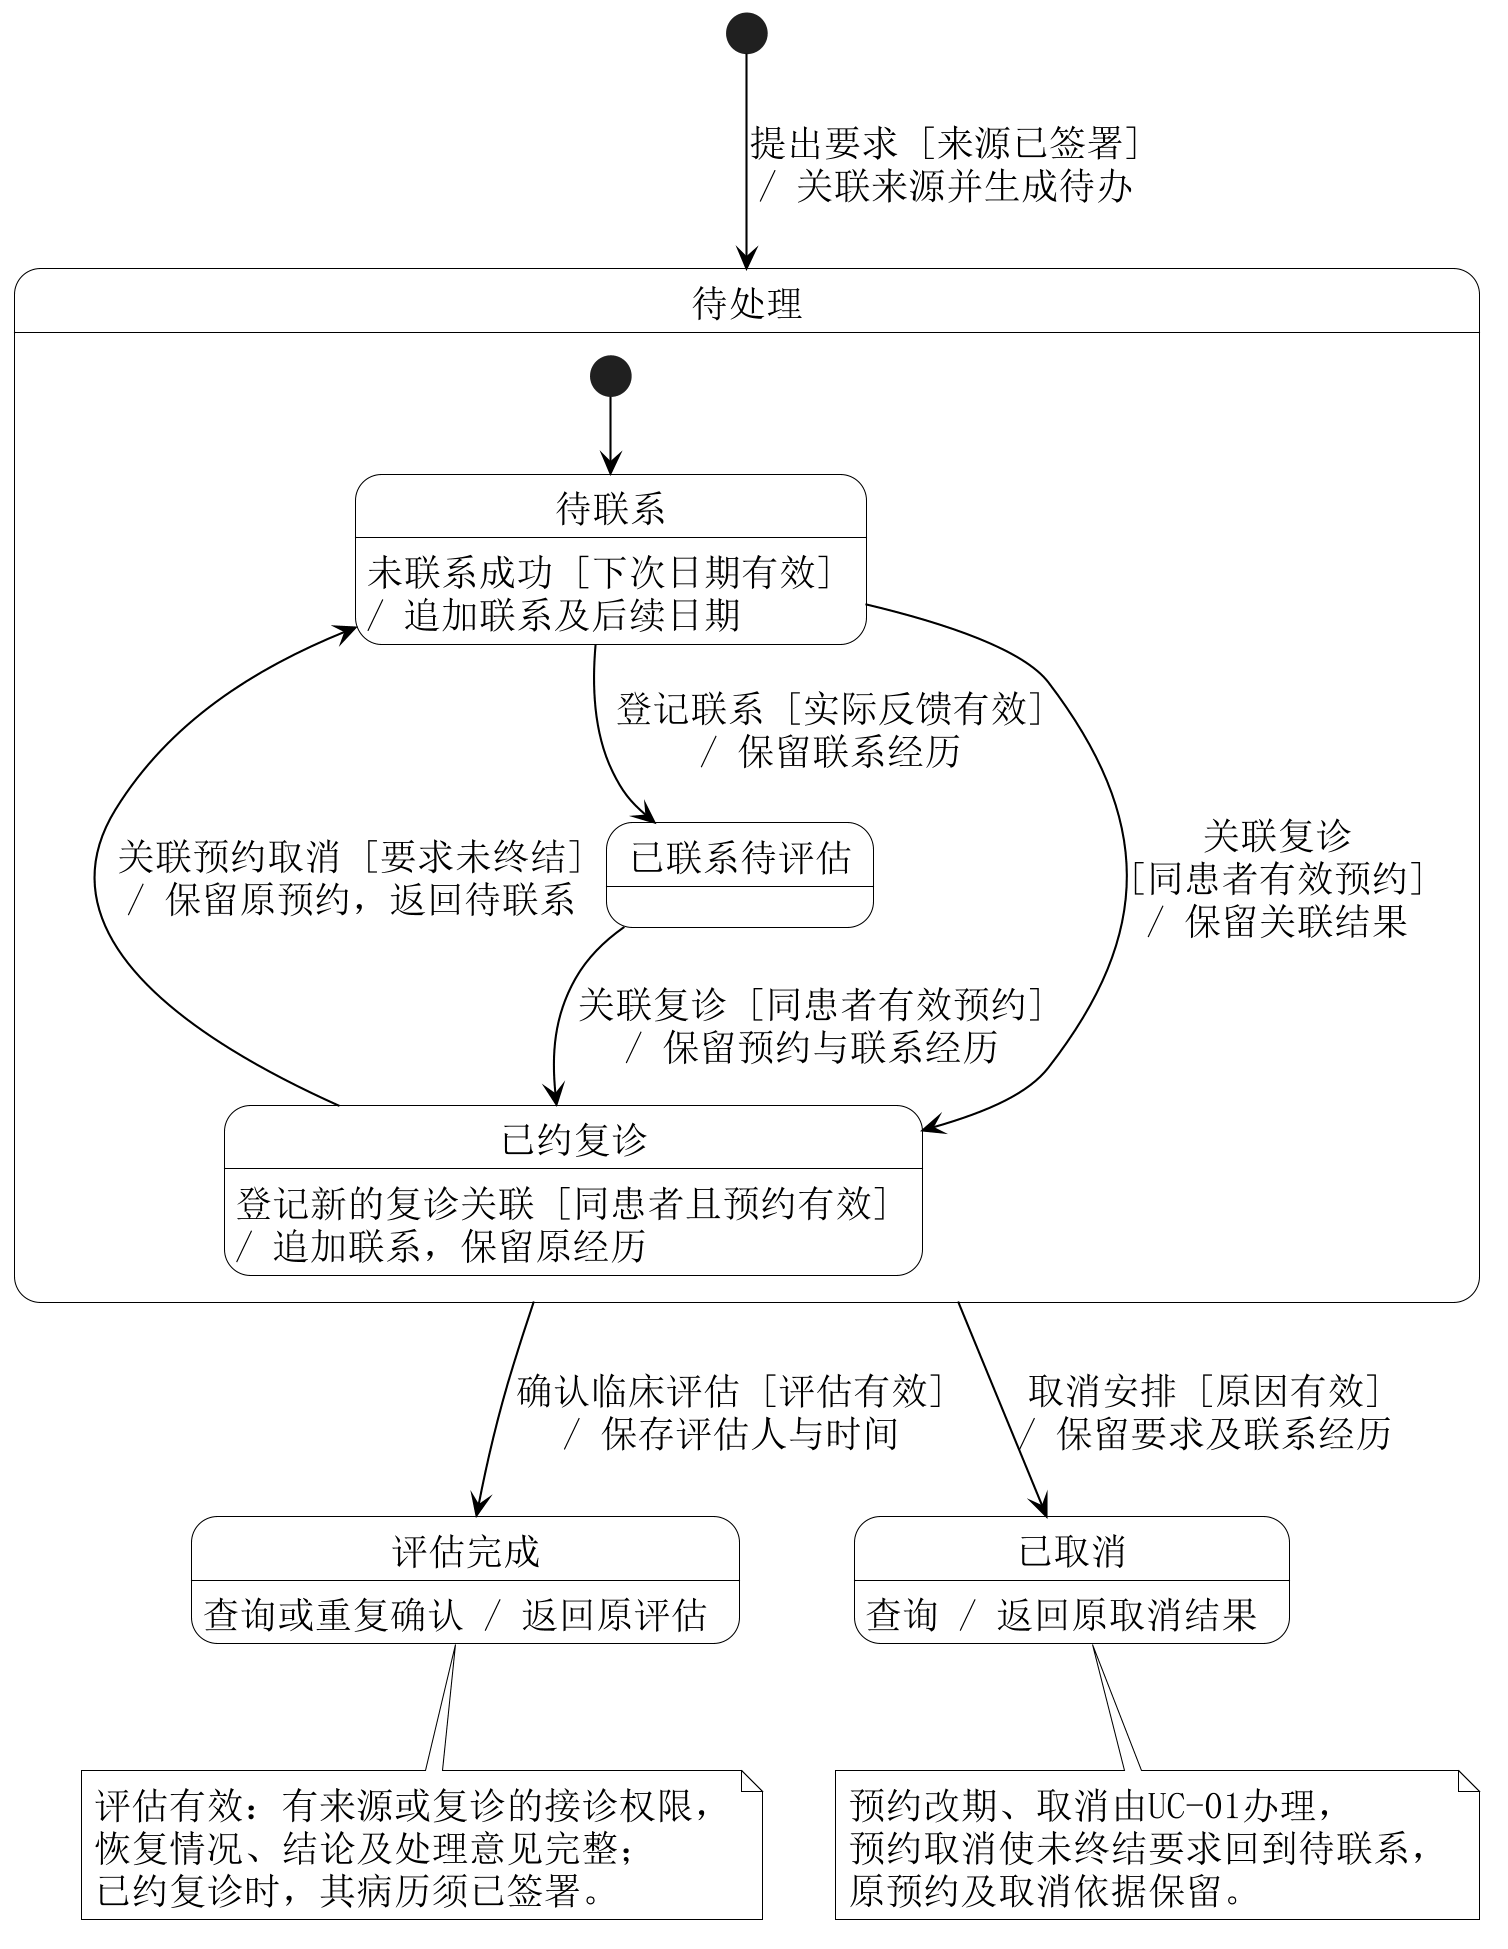
\includegraphics[width=\textwidth,height=18cm,keepaspectratio]{diagrams/17-followup-state-machine.png}
\caption{诊后要求的状态机图}
\label{fig:17-followup-state-machine}
\end{figure}
\clearpage
\subsubsection{方案项目的状态机图}

患者决定由牙医在UC-10中记录。实际项目只有符合已同意及剩余数量条件才能引用该方案；UC-04保存实际完成明细。签署后需要新方案时，在后续就诊形成新的方案对象，原方案仍保留。
\begin{figure}[!htbp]
\centering
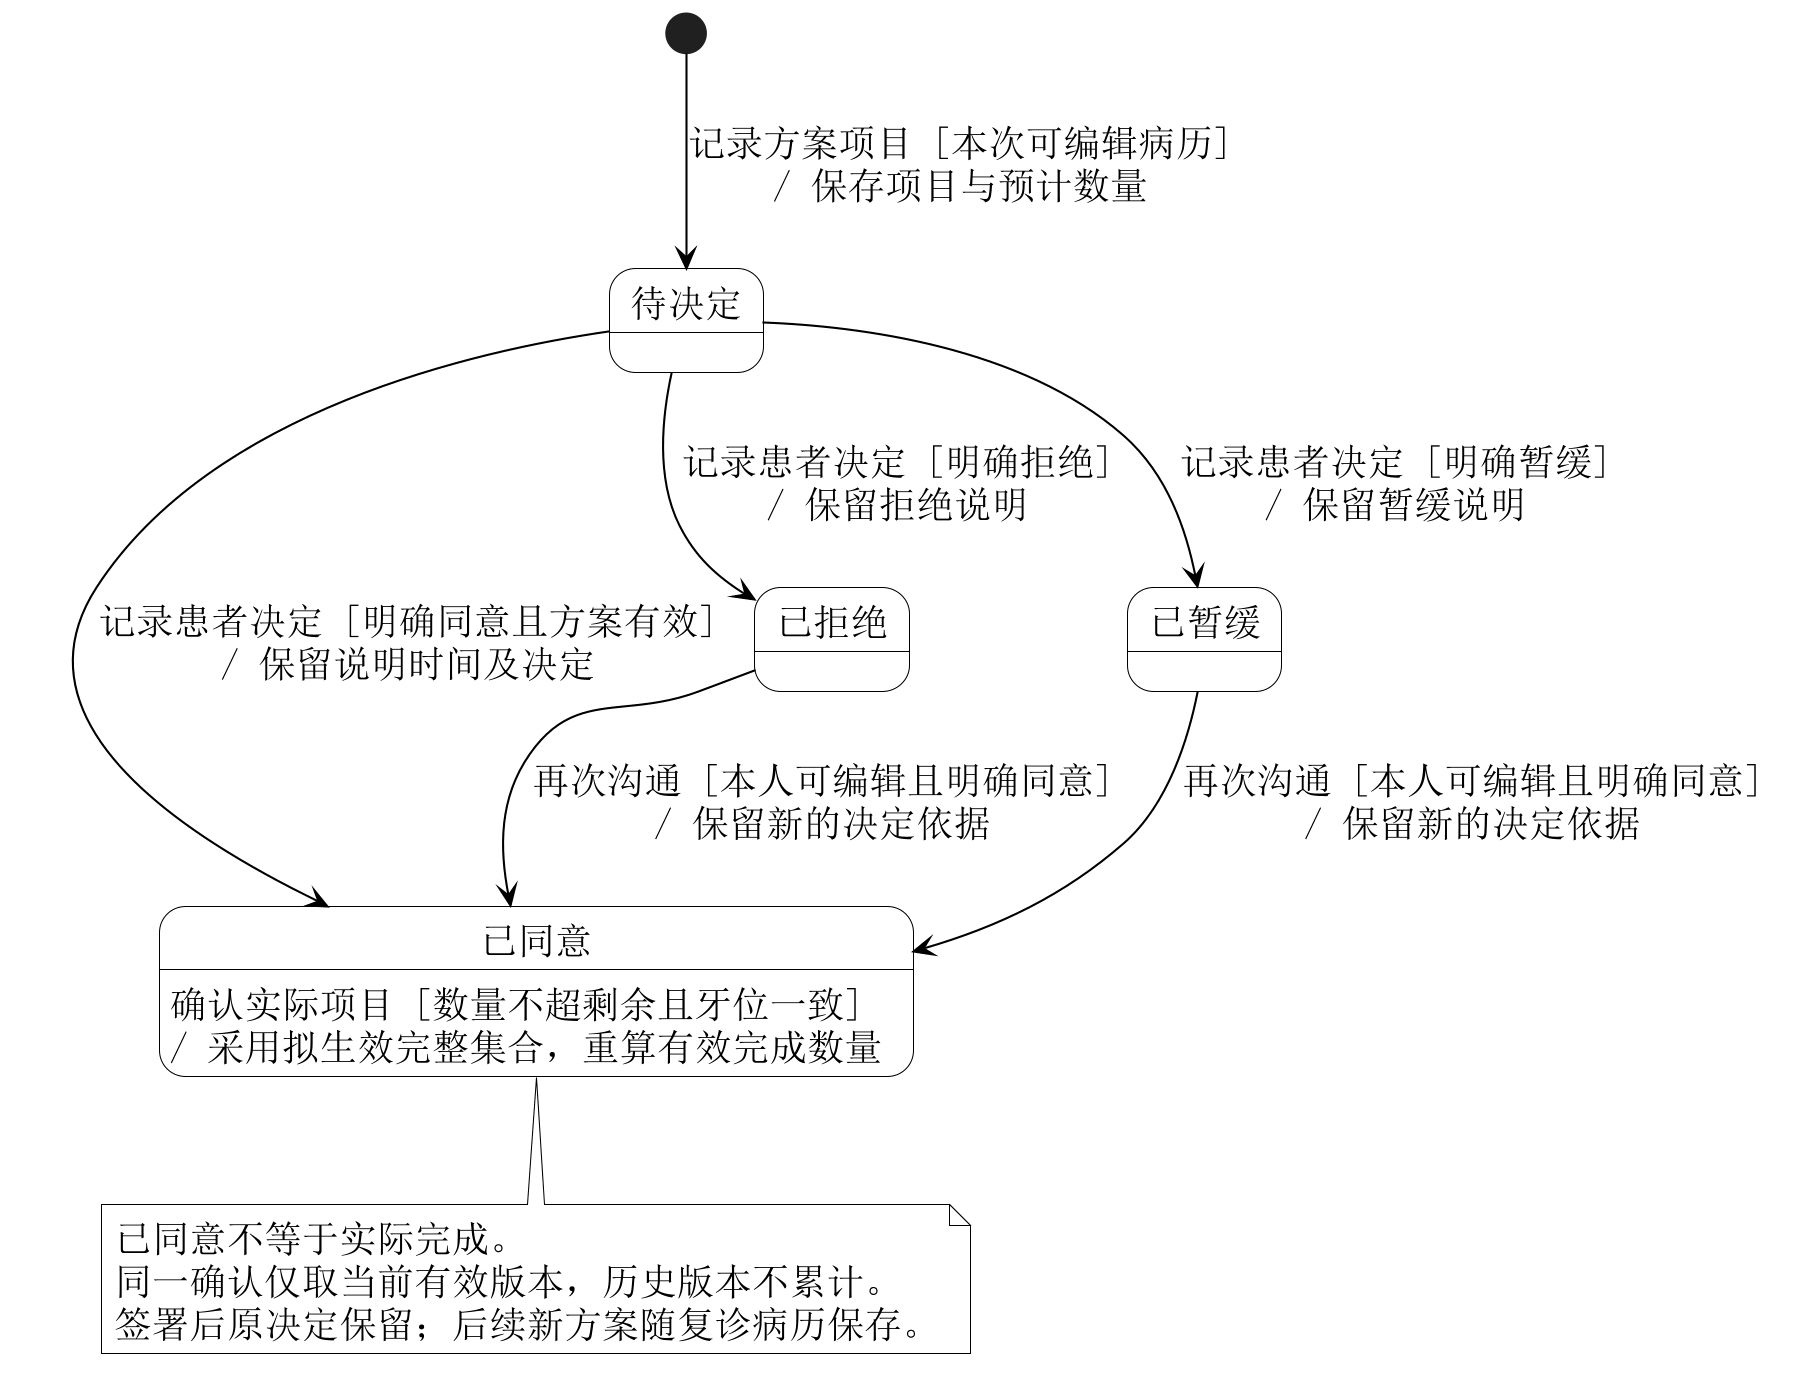
\includegraphics[width=\textwidth,height=18cm,keepaspectratio]{diagrams/18-plan-item-state-machine.png}
\caption{方案项目的状态机图}
\label{fig:18-plan-item-state-machine}
\end{figure}
\clearpage
\subsubsection{状态条件与用例对应}

就诊登记后尚无当前诊疗确认，处于未确认项目；有当前确认但任一明细缺少适用价目时，处于已确认缺价；当前确认的全部明细具备适用价目且尚无有效收款时，处于可结算；关联有效现金收款后，处于已结清。可结算仅说明对象具备计费条件，收款请求仍须通过最终核验。

\begin{table}[!htbp]
\centering
\caption{就诊状态机的警戒条件}
\label{tab:state-guards}
\small
\renewcommand{\arraystretch}{1.25}
\begin{tabularx}{\textwidth}{@{}p{2.3cm}L@{}}
\toprule
图中条件 & 必须同时满足的业务条件 \\
\midrule
预约可到诊 & 对应预约为当日已预约，身份已核对，尚无关联就诊；创建就诊与预约关联同时生效。 \\
确认有效 & 操作者为本次接诊牙医，项目为实际完成且有效的收费项目，明细非空，数量为正整数；保存前确认当前内容未被他人改变。同一项目和牙位且方案、计价及完成日期依据一致的重复明细合并数量。 \\
更正有效 & 尚未结清，由本次接诊牙医提交完整项目集合及更正原因；符合确认有效的项目、数量和版本条件。原确认及其明细保留。 \\
全部明细已有适用价目 & 每条明细均关联其计价时点适用的价目；既有同项目明细更正时继承原时点及价目，新增或更换项目使用本次确认时点；缺价补齐按保存的计价时点，既有单价不被后续调价覆盖。 \\
结算有效 & 本次就诊尚未结清，当前项目与价目完整，提交的核对依据与当前确认版本及价目依据一致；现金金额有效且不少于应收金额。生效前再次核验，现金收款及结清同时生效。 \\
\bottomrule
\end{tabularx}
\end{table}

\begin{table}[!htbp]
\centering
\caption{状态机与用例、分析责任对应}
\label{tab:state-usecases}
\small
\renewcommand{\arraystretch}{1.2}
\begin{tabularx}{\textwidth}{@{}p{1.6cm}L@{}}
\toprule
用例 & 对象状态及操作责任 \\
\midrule
UC-01 & 预约新增进入已预约；调整为内部迁移；取消进入已取消，预约变更保留原安排及原因。 \\
UC-02 & 查询预约及安排；不改变预约状态。 \\
UC-03 & 预约由已预约变为已到诊，唯一就诊进入未确认项目；重复请求读取原就诊。 \\
UC-04 & 就诊组织诊疗确认及明细；首次确认或更正后按价目完整性进入已确认缺价或可结算。 \\
UC-05 & 收费项目组织价目版本；可供缺价明细按其计价时点确定计价依据，已关联历史单价保持不变。 \\
UC-06 & 诊疗确认委托明细计算并汇总；未确认或缺价时不能完成核对，查询本身不改变就诊状态。 \\
UC-07 & 有效结算使就诊进入已结清；现金收款计算找零并形成收据，重复请求返回原收款。 \\
\bottomrule
\end{tabularx}
\end{table}

\clearpage
\begin{table}[!htbp]
\centering
\caption{对象生命周期与业务约束}
\label{tab:new-state-guards}
\small
\renewcommand{\arraystretch}{1.18}
\begin{tabularx}{\textwidth}{@{}>{\raggedright\arraybackslash}p{2.6cm}>{\raggedright\arraybackslash}p{2.9cm}L@{}}
\toprule
对象 & 用例 & 迁移及约束 \\
\midrule
病历 & UC-10、11 & 草稿允许本人编辑；完整签署后保留原文；补充追加原因及内容，不影响原收费依据。 \\
方案项目 & UC-10、04 & 待决定、拒绝、暂缓不作为治疗许可；已同意项目仍须核对本次就诊、牙位和剩余数量。 \\
诊后要求 & UC-12、13、14 & 提出要求进入待联系；关联预约取消后，未终结要求回到待联系；牙医临床确认才完成，取消要求须另行保留原因。 \\
接诊时段 & UC-15、16 & 发布前须支持相关有效预约；查询不建立或更改预约。 \\
材料 & UC-17、18 & 库存由原始变动得到；领用后数量不少于零，盘点须负责人确认，查询不改变余额。 \\
现金收款及核对 & UC-19、20 & 统计按实际日期；核对保留原收款依据及差异说明，不改写原凭据。 \\
\bottomrule
\end{tabularx}
\end{table}

未满足警戒条件的请求返回规约中的原因并保持原有效内容。缺价明细逐项确定计价依据时，只有全部补齐才进入可结算；价目维护本身不直接改变历史确认。结果未收到时先查询既有到诊或收款，再按规约恢复，通讯结果不另设为预约或就诊的业务状态。

\end{document}
